% poster_example_2.tex
%
% Another example poster
%
% Copyright (c) 2017 Dennis Ogbe <dogbe@purdue.edu>
%
% This file is published under the Creative Commons Attribution-NonCommercial
% 4.0 International License. For more information, please visit
% https://creativecommons.org/licenses/by-nc/4.0/

% Sometimes these commands help with Adobe reader
\pdfobjcompresslevel=0
\pdfminorversion=4

\documentclass[pdf]{beamer}

% beamerposter
\usepackage[orientation=portrait,size=custom,width=60.96,height=91.44, scale=1.35]{beamerposter}

\usepackage{framed}
\usepackage{cmbright}
\usepackage{filecontents}

% bibliography
\begin{filecontents}{\jobname.bib}
@article{journal_paper,
	title = "{Noisy Beam Alignment Techniques for Reciprocal MIMO Channels}",
	journal = {(in press) IEEE Trans. Sig. Proc. (arXiv:1609.03601 [cs.IT])},
	author = {D. Ogbe and D. J. Love and V. Raghavan},
	year = 2017,
}
@inproceedings{conference_paper,
	title = {{Iterative} {Beam} {Alignment} {Algorithms} for {TDD} {MIMO} {Channels}},
	booktitle = {2017 {IEEE} {International} {Conference} on {Acoustics}, {Speech}, and {Signal} {Processing} ({ICASSP})},
	author = {D. Ogbe and D. J. Love and V. Raghavan},
	year = 2017,
	month = Mar.,
  pages = {3469--3473}
}

\end{filecontents}
\usepackage[bibstyle=ieee,citestyle=numeric,backend=biber]{biblatex}
\addbibresource{\jobname.bib}
% if the following were not set, biblatex would try to insert a section on
% every frame, which breaks beamer
\defbibheading{bibliography}[\bibname]{}
% modify the font size of the \cite commands
% we want numbers instead of symbols in the bibliography
\setbeamertemplate{bibliography item}[text]
% make it small
\renewcommand*{\bibfont}{\footnotesize}

% useful to set this when using Inkscape SVG figures
\graphicspath{{./figures/}}

\usetheme{purduegoldposter}


% set title and author
\title{Noisy Beam Alignment Techniques for Reciprocal \\ MIMO Channels}
\subtitle{NASIT 2017, Atlanta, GA}
\author{Dennis Ogbe$^{*}$, David J. Love$^{*}$, Vasanthan Raghavan$^{\dagger}$}
\date{June 5-9, 2017}


\begin{document}
\begin{frame}[t]
% title
\begin{textblock}{1}(0,0)
  \begin{tcolorbox}[
    % colors
    colback=MoonDustGray,
    colframe=black,
    % lower and upper side by side
    sidebyside,
    lower separated=false,
    % 80% for title, 20% for logos
    righthand width=0.2\paperwidth,
    % rule widths & arcs
    toprule=0pt,
    leftrule=0pt,
    rightrule=0pt,
    bottomrule=0.3in,
    arc=0pt,
    % padding
    % boxsep=0.2in,
    % text & logo alignment
    halign upper=right,
    halign lower=left,
    ]
    \Large{\textbf{\inserttitle}}

    \large{\emph{\insertauthor}}

    \small{$^{*}$Purdue University, School of Electrical and Computer Engineering, West Lafayette, IN 47907, USA}

    \small{$^{\dagger}$Qualcomm, Inc., Bridgewater, NJ 08807, USA}
    \tcblower
    \begin{center}
      
\includegraphics[width=4.5in]{./logos/Purdue-Sig-Black-cmyk.pdf}
    \end{center}

    
\includegraphics[width=2.2in]{./logos/nsf4.pdf}
    \hfill
   \raisebox{0.2in}{
\includegraphics[width=2in]{./logos/CSoI-logo-print.png}}
\end{tcolorbox}
\end{textblock}

% all of the boxes in one raster
\begin{textblock}{0.98}(0.01,0.121)
  \begin{tcbraster}[%
    raster columns = 2,
    raster column skip = 0.01\paperwidth,
    raster row skip = 0.01\paperwidth,
    raster equal height=rows
    ]%
    % background/beam-based sounding
    \begin{mybox}[%
      lefthand ratio=0.5,
      sidebyside align=top seam,
      raster multicolumn=2
      ]{Background}
      \settowidth{\leftmargini}{\usebeamertemplate{itemize item}}
      \addtolength{\leftmargini}{\labelsep}
      \begin{itemize}
      \item 5G technologies (mmWave \& massive MIMO) rely on \textbf{beamforming gains} to realize data rate requirements
      \item However: \textbf{Optimal beamforming weights depend on the channel matrix}
      \end{itemize}
      \begin{center}
        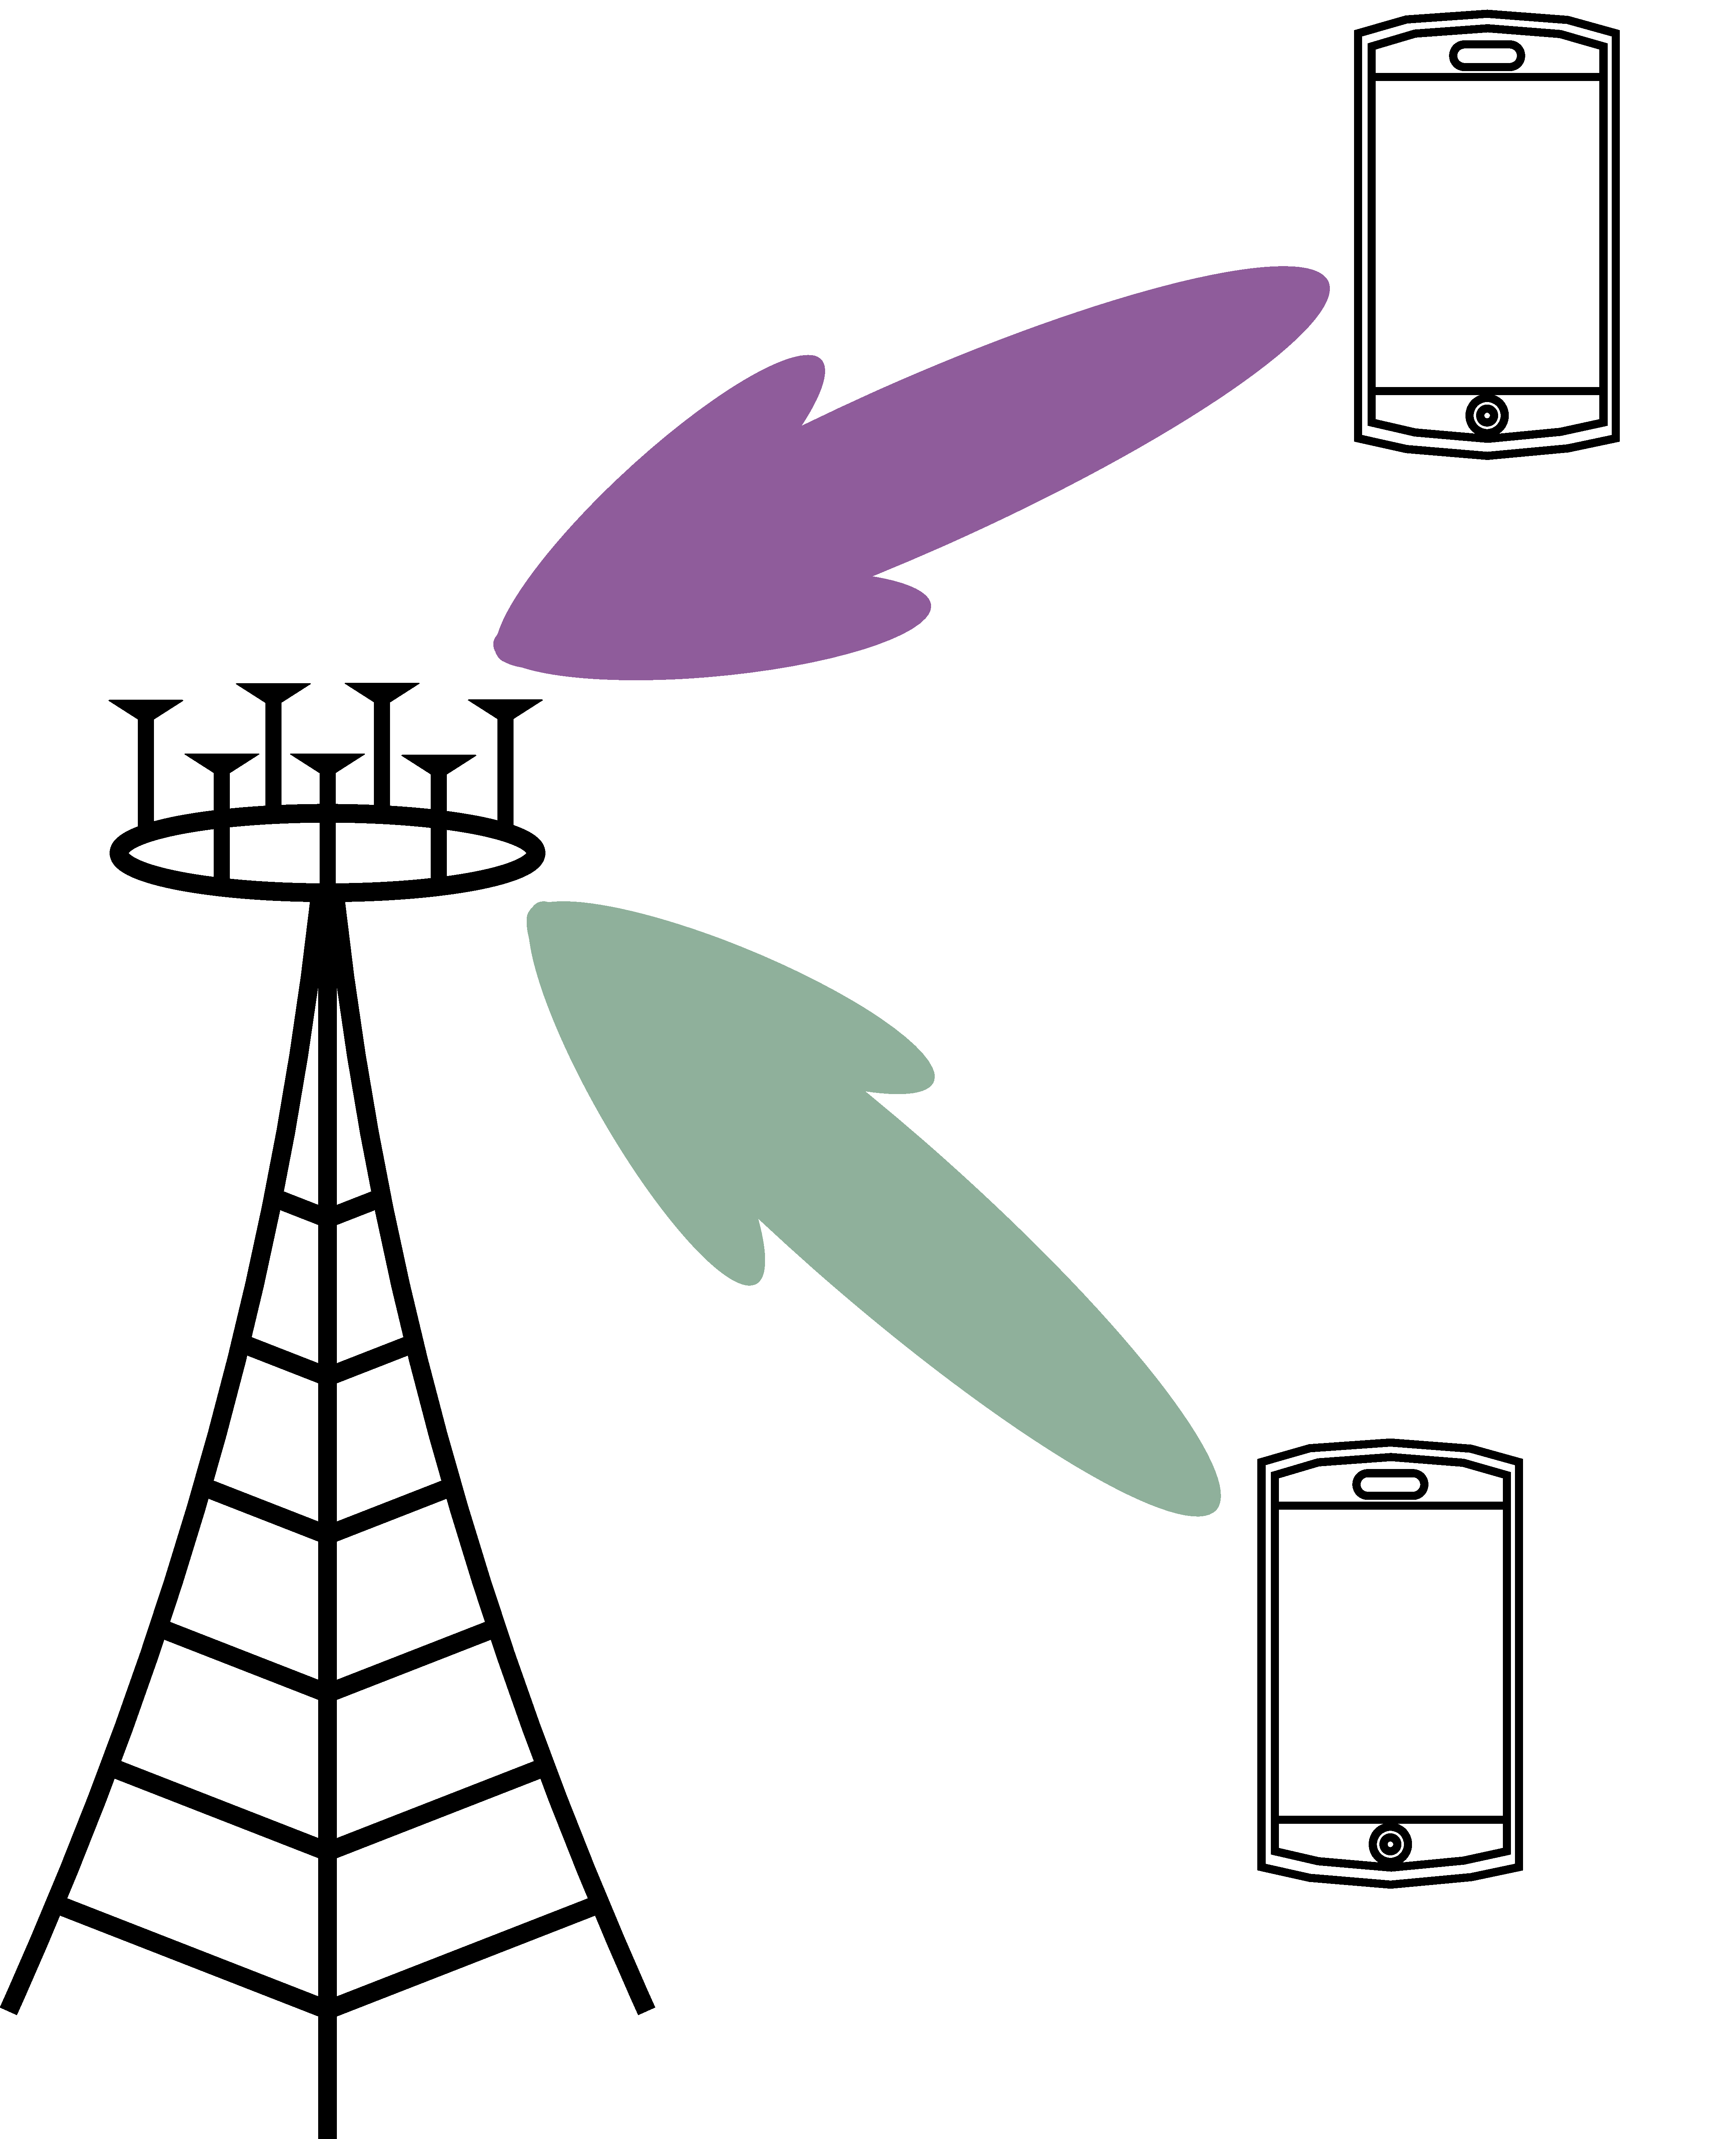
\includegraphics[width=0.25\textwidth]{./figures/beamforming.pdf}
        \hspace*{1.3in}
        %\includegraphics[width=0.6\textwidth]{./figures/beamforming_model.pdf}
         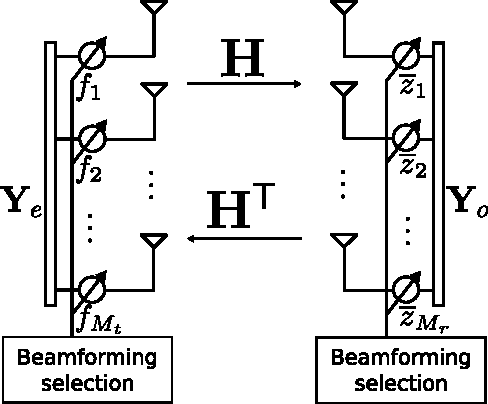
\includegraphics[width=0.4\textwidth]{./figures/sysmodel/system_model.pdf}
    \end{center}
    \tcblower
      \settowidth{\leftmargini}{\usebeamertemplate{itemize item}}
      \addtolength{\leftmargini}{\labelsep}
      \begin{itemize}
      \item Traditional CSI acquisition (Sounding sequences $\rightarrow$ CSI feedback $\rightarrow$ SVD) is impractical with many antennas
      \item Solution: \textbf{Beam-based sounding}
        \begin{itemize}
        \item Users always transmit on beams
        \item Acquire beamformers using a TDD \textbf{beam alignment phase}
        \item Exploit reciprocity of the wireless channel
        \end{itemize}
      \item \textbf{Need for \underline{practical} approaches to TDD-based beam alignment}
        \begin{itemize}
        \item Additive noise
        \item mmWave channel models
        \item Low overhead
        \end{itemize}
      \end{itemize}
  \end{mybox}

  % ping-pong beam alignment
  \begin{mybox}[lower separated=false,sidebyside=false]{Ping-pong beam alignment}
    \settowidth{\leftmargini}{\usebeamertemplate{itemize item}}
    \addtolength{\leftmargini}{\labelsep}
    \begin{itemize}
    \item Divide each channel~use~$k$ into two time slots
    \item Communication nodes sound beams in their half of the slots
    \end{itemize}
    \tcblower
    \emph{Ping:} Node 1 sounds beam $\mathbf{f}[k]$ as \vspace*{-6pt}
    \begin{IEEEeqnarray*}{rCl}
      \label{eq:slot1_obs}
      \mathbf{y}_{o}[k] = \sqrt{\rho_o}\, \mathbf{H}\mathbf{f}[k] + \mathbf{n}_{o}[k]
    \end{IEEEeqnarray*}

    \emph{Pong:} Node 2 sounds beam $\mathbf{z}[k]$ as \vspace*{-6pt}
    \begin{IEEEeqnarray*}{rCl}
      \label{eq:slot2_obs}
      \mathbf{y}_{e}[k] = \sqrt{\rho_e}\, \mathbf{H}^{\T}\conj{\mathbf{z}}[k] + \mathbf{n}_{e}[k]
    \end{IEEEeqnarray*}

    \vspace*{0.1in}
    \small{\underline{Notation:} $\mathbf{H}$\ ---\ $M_r \times M_t$ channel matrix, $\rho_{e}, \rho_{o}$\ ---\ beam alignment SNR, $\mathbf{n}_{e}[k], \mathbf{n}_{o}[k]$\ ---\ complex additive white Gaussian noise}
  \end{mybox}
  % power method
  \begin{mybox}[%
    lefthand ratio=0.5,
    sidebyside align=top seam,
    ]{Power Method}
    \settowidth{\leftmargini}{\usebeamertemplate{itemize item}}
    \addtolength{\leftmargini}{\labelsep}
    \begin{itemize}
    \item We propose new beam alignment algorithms based on the \textbf{power method}
    \item Good performance for the noiseless case
    \item \textbf{Convergence can slow down dramatically under additive noise}
    \end{itemize}
    \tcblower
    \begin{center}
      \small{\emph{Example: One-way Power Method}}
    \end{center}
    \resizebox{\textwidth}{!}{%% Creator: Matplotlib, PGF backend
%%
%% To include the figure in your LaTeX document, write
%%   \input{<filename>.pgf}
%%
%% Make sure the required packages are loaded in your preamble
%%   \usepackage{pgf}
%%
%% Figures using additional raster images can only be included by \input if
%% they are in the same directory as the main LaTeX file. For loading figures
%% from other directories you can use the `import` package
%%   \usepackage{import}
%% and then include the figures with
%%   \import{<path to file>}{<filename>.pgf}
%%
%% Matplotlib used the following preamble
%%   \usepackage[utf8x]{inputenc}
%%   \usepackage[T1]{fontenc}
%%
\begingroup%
\makeatletter%
\begin{pgfpicture}%
\pgfpathrectangle{\pgfpointorigin}{\pgfqpoint{2.546008in}{1.018403in}}%
\pgfusepath{use as bounding box, clip}%
\begin{pgfscope}%
\pgfsetbuttcap%
\pgfsetmiterjoin%
\pgfsetlinewidth{0.000000pt}%
\definecolor{currentstroke}{rgb}{0.000000,0.000000,0.000000}%
\pgfsetstrokecolor{currentstroke}%
\pgfsetstrokeopacity{0.000000}%
\pgfsetdash{}{0pt}%
\pgfpathmoveto{\pgfqpoint{0.000000in}{0.000000in}}%
\pgfpathlineto{\pgfqpoint{2.546008in}{0.000000in}}%
\pgfpathlineto{\pgfqpoint{2.546008in}{1.018403in}}%
\pgfpathlineto{\pgfqpoint{0.000000in}{1.018403in}}%
\pgfpathclose%
\pgfusepath{}%
\end{pgfscope}%
\begin{pgfscope}%
\pgfsetroundcap%
\pgfsetroundjoin%
\definecolor{currentfill}{rgb}{1.000000,0.000000,0.000000}%
\pgfsetfillcolor{currentfill}%
\pgfsetlinewidth{1.003750pt}%
\definecolor{currentstroke}{rgb}{1.000000,0.000000,0.000000}%
\pgfsetstrokecolor{currentstroke}%
\pgfsetdash{}{0pt}%
\pgfpathmoveto{\pgfqpoint{1.430304in}{0.237593in}}%
\pgfpathquadraticcurveto{\pgfqpoint{0.980228in}{0.497445in}}{\pgfqpoint{0.530151in}{0.757297in}}%
\pgfpathlineto{\pgfqpoint{0.519040in}{0.738052in}}%
\pgfpathquadraticcurveto{\pgfqpoint{0.513955in}{0.757025in}}{\pgfqpoint{0.508870in}{0.775999in}}%
\pgfpathquadraticcurveto{\pgfqpoint{0.527844in}{0.781082in}}{\pgfqpoint{0.546818in}{0.786165in}}%
\pgfpathlineto{\pgfqpoint{0.535707in}{0.766920in}}%
\pgfpathquadraticcurveto{\pgfqpoint{0.985783in}{0.507068in}}{\pgfqpoint{1.435860in}{0.247216in}}%
\pgfpathlineto{\pgfqpoint{1.430304in}{0.237593in}}%
\pgfpathclose%
\pgfusepath{stroke,fill}%
\end{pgfscope}%
\begin{pgfscope}%
\definecolor{textcolor}{rgb}{1.000000,0.000000,0.000000}%
\pgfsetstrokecolor{textcolor}%
\pgfsetfillcolor{textcolor}%
\pgftext[x=0.722308in,y=0.775999in,,]{\color{textcolor}\rmfamily\fontsize{9.000000}{10.800000}\selectfont \(\displaystyle \mathbf{s}_{1}\)}%
\end{pgfscope}%
\begin{pgfscope}%
\pgfsetroundcap%
\pgfsetroundjoin%
\definecolor{currentfill}{rgb}{0.000000,0.000000,1.000000}%
\pgfsetfillcolor{currentfill}%
\pgfsetlinewidth{1.003750pt}%
\definecolor{currentstroke}{rgb}{0.000000,0.000000,1.000000}%
\pgfsetstrokecolor{currentstroke}%
\pgfsetdash{}{0pt}%
\pgfpathmoveto{\pgfqpoint{1.430304in}{0.247216in}}%
\pgfpathquadraticcurveto{\pgfqpoint{1.880381in}{0.507068in}}{\pgfqpoint{2.330458in}{0.766920in}}%
\pgfpathlineto{\pgfqpoint{2.319346in}{0.786165in}}%
\pgfpathquadraticcurveto{\pgfqpoint{2.338320in}{0.781082in}}{\pgfqpoint{2.357294in}{0.775999in}}%
\pgfpathquadraticcurveto{\pgfqpoint{2.352209in}{0.757025in}}{\pgfqpoint{2.347124in}{0.738052in}}%
\pgfpathlineto{\pgfqpoint{2.336013in}{0.757297in}}%
\pgfpathquadraticcurveto{\pgfqpoint{1.885937in}{0.497445in}}{\pgfqpoint{1.435860in}{0.237593in}}%
\pgfpathlineto{\pgfqpoint{1.430304in}{0.247216in}}%
\pgfpathclose%
\pgfusepath{stroke,fill}%
\end{pgfscope}%
\begin{pgfscope}%
\definecolor{textcolor}{rgb}{0.000000,0.000000,1.000000}%
\pgfsetstrokecolor{textcolor}%
\pgfsetfillcolor{textcolor}%
\pgftext[x=2.449715in,y=0.829358in,,]{\color{textcolor}\rmfamily\fontsize{9.000000}{10.800000}\selectfont \(\displaystyle \mathbf{s}_{2}\)}%
\end{pgfscope}%
\begin{pgfscope}%
\pgfsetroundcap%
\pgfsetroundjoin%
\definecolor{currentfill}{rgb}{0.000000,0.000000,0.000000}%
\pgfsetfillcolor{currentfill}%
\pgfsetlinewidth{1.003750pt}%
\definecolor{currentstroke}{rgb}{0.000000,0.000000,0.000000}%
\pgfsetstrokecolor{currentstroke}%
\pgfsetdash{}{0pt}%
\pgfpathmoveto{\pgfqpoint{1.433719in}{0.236886in}}%
\pgfpathquadraticcurveto{\pgfqpoint{0.917446in}{0.177272in}}{\pgfqpoint{0.401173in}{0.117658in}}%
\pgfpathlineto{\pgfqpoint{0.403722in}{0.095582in}}%
\pgfpathquadraticcurveto{\pgfqpoint{0.388330in}{0.107786in}}{\pgfqpoint{0.372939in}{0.119990in}}%
\pgfpathquadraticcurveto{\pgfqpoint{0.385144in}{0.135380in}}{\pgfqpoint{0.397349in}{0.150771in}}%
\pgfpathlineto{\pgfqpoint{0.399898in}{0.128695in}}%
\pgfpathquadraticcurveto{\pgfqpoint{0.916172in}{0.188309in}}{\pgfqpoint{1.432445in}{0.247924in}}%
\pgfpathlineto{\pgfqpoint{1.433719in}{0.236886in}}%
\pgfpathclose%
\pgfusepath{stroke,fill}%
\end{pgfscope}%
\begin{pgfscope}%
\pgftext[x=0.213917in,y=0.101628in,,]{\rmfamily\fontsize{9.000000}{10.800000}\selectfont \(\displaystyle \mathbf{v}^{(0)}\)}%
\end{pgfscope}%
\begin{pgfscope}%
\pgfsetroundcap%
\pgfsetroundjoin%
\definecolor{currentfill}{rgb}{0.000000,0.000000,0.000000}%
\pgfsetfillcolor{currentfill}%
\pgfsetlinewidth{1.003750pt}%
\definecolor{currentstroke}{rgb}{0.000000,0.000000,0.000000}%
\pgfsetstrokecolor{currentstroke}%
\pgfsetdash{}{0pt}%
\pgfpathmoveto{\pgfqpoint{1.432672in}{0.236864in}}%
\pgfpathquadraticcurveto{\pgfqpoint{0.914389in}{0.275269in}}{\pgfqpoint{0.396106in}{0.313673in}}%
\pgfpathlineto{\pgfqpoint{0.394464in}{0.291512in}}%
\pgfpathquadraticcurveto{\pgfqpoint{0.381638in}{0.306389in}}{\pgfqpoint{0.368812in}{0.321267in}}%
\pgfpathquadraticcurveto{\pgfqpoint{0.383691in}{0.334091in}}{\pgfqpoint{0.398569in}{0.346916in}}%
\pgfpathlineto{\pgfqpoint{0.396927in}{0.324754in}}%
\pgfpathquadraticcurveto{\pgfqpoint{0.915210in}{0.286350in}}{\pgfqpoint{1.433493in}{0.247945in}}%
\pgfpathlineto{\pgfqpoint{1.432672in}{0.236864in}}%
\pgfpathclose%
\pgfusepath{stroke,fill}%
\end{pgfscope}%
\begin{pgfscope}%
\pgftext[x=0.209172in,y=0.333096in,,]{\rmfamily\fontsize{9.000000}{10.800000}\selectfont \(\displaystyle \mathbf{v}^{(1)}\)}%
\end{pgfscope}%
\begin{pgfscope}%
\pgfsetroundcap%
\pgfsetroundjoin%
\definecolor{currentfill}{rgb}{0.000000,0.000000,0.000000}%
\pgfsetfillcolor{currentfill}%
\pgfsetlinewidth{1.003750pt}%
\definecolor{currentstroke}{rgb}{0.000000,0.000000,0.000000}%
\pgfsetstrokecolor{currentstroke}%
\pgfsetdash{}{0pt}%
\pgfpathmoveto{\pgfqpoint{1.431741in}{0.237013in}}%
\pgfpathquadraticcurveto{\pgfqpoint{0.927402in}{0.362446in}}{\pgfqpoint{0.423062in}{0.487879in}}%
\pgfpathlineto{\pgfqpoint{0.417698in}{0.466313in}}%
\pgfpathquadraticcurveto{\pgfqpoint{0.407571in}{0.483144in}}{\pgfqpoint{0.397443in}{0.499975in}}%
\pgfpathquadraticcurveto{\pgfqpoint{0.414275in}{0.510101in}}{\pgfqpoint{0.431107in}{0.520226in}}%
\pgfpathlineto{\pgfqpoint{0.425744in}{0.498661in}}%
\pgfpathquadraticcurveto{\pgfqpoint{0.930083in}{0.373229in}}{\pgfqpoint{1.434423in}{0.247796in}}%
\pgfpathlineto{\pgfqpoint{1.431741in}{0.237013in}}%
\pgfpathclose%
\pgfusepath{stroke,fill}%
\end{pgfscope}%
\begin{pgfscope}%
\pgftext[x=0.242098in,y=0.538610in,,]{\rmfamily\fontsize{9.000000}{10.800000}\selectfont \(\displaystyle \mathbf{v}^{(2)}\)}%
\end{pgfscope}%
\begin{pgfscope}%
\pgfsetroundcap%
\pgfsetroundjoin%
\definecolor{currentfill}{rgb}{0.000000,0.000000,0.000000}%
\pgfsetfillcolor{currentfill}%
\pgfsetlinewidth{1.003750pt}%
\definecolor{currentstroke}{rgb}{0.000000,0.000000,0.000000}%
\pgfsetstrokecolor{currentstroke}%
\pgfsetdash{}{0pt}%
\pgfpathmoveto{\pgfqpoint{1.431104in}{0.237213in}}%
\pgfpathquadraticcurveto{\pgfqpoint{0.945454in}{0.422242in}}{\pgfqpoint{0.459804in}{0.607271in}}%
\pgfpathlineto{\pgfqpoint{0.451892in}{0.586505in}}%
\pgfpathquadraticcurveto{\pgfqpoint{0.443857in}{0.604429in}}{\pgfqpoint{0.435821in}{0.622353in}}%
\pgfpathquadraticcurveto{\pgfqpoint{0.453746in}{0.630387in}}{\pgfqpoint{0.471671in}{0.638420in}}%
\pgfpathlineto{\pgfqpoint{0.463760in}{0.617654in}}%
\pgfpathquadraticcurveto{\pgfqpoint{0.949410in}{0.432625in}}{\pgfqpoint{1.435060in}{0.247596in}}%
\pgfpathlineto{\pgfqpoint{1.431104in}{0.237213in}}%
\pgfpathclose%
\pgfusepath{stroke,fill}%
\end{pgfscope}%
\begin{pgfscope}%
\pgftext[x=0.286232in,y=0.679346in,,]{\rmfamily\fontsize{9.000000}{10.800000}\selectfont \(\displaystyle \mathbf{v}^{(3)}\)}%
\end{pgfscope}%
\begin{pgfscope}%
\pgfsetroundcap%
\pgfsetroundjoin%
\definecolor{currentfill}{rgb}{0.000000,0.000000,0.000000}%
\pgfsetfillcolor{currentfill}%
\pgfsetlinewidth{1.003750pt}%
\definecolor{currentstroke}{rgb}{0.000000,0.000000,0.000000}%
\pgfsetstrokecolor{currentstroke}%
\pgfsetdash{}{0pt}%
\pgfpathmoveto{\pgfqpoint{1.430731in}{0.237371in}}%
\pgfpathquadraticcurveto{\pgfqpoint{0.959869in}{0.457327in}}{\pgfqpoint{0.489007in}{0.677284in}}%
\pgfpathlineto{\pgfqpoint{0.479601in}{0.657150in}}%
\pgfpathquadraticcurveto{\pgfqpoint{0.472895in}{0.675612in}}{\pgfqpoint{0.466188in}{0.694075in}}%
\pgfpathquadraticcurveto{\pgfqpoint{0.484651in}{0.700779in}}{\pgfqpoint{0.503114in}{0.707484in}}%
\pgfpathlineto{\pgfqpoint{0.493709in}{0.687350in}}%
\pgfpathquadraticcurveto{\pgfqpoint{0.964571in}{0.467394in}}{\pgfqpoint{1.435433in}{0.247438in}}%
\pgfpathlineto{\pgfqpoint{1.430731in}{0.237371in}}%
\pgfpathclose%
\pgfusepath{stroke,fill}%
\end{pgfscope}%
\begin{pgfscope}%
\pgfsetroundcap%
\pgfsetroundjoin%
\definecolor{currentfill}{rgb}{0.000000,0.000000,0.000000}%
\pgfsetfillcolor{currentfill}%
\pgfsetlinewidth{1.003750pt}%
\definecolor{currentstroke}{rgb}{0.000000,0.000000,0.000000}%
\pgfsetstrokecolor{currentstroke}%
\pgfsetdash{}{0pt}%
\pgfpathmoveto{\pgfqpoint{1.430528in}{0.237471in}}%
\pgfpathquadraticcurveto{\pgfqpoint{0.969029in}{0.476451in}}{\pgfqpoint{0.507531in}{0.715430in}}%
\pgfpathlineto{\pgfqpoint{0.497312in}{0.695697in}}%
\pgfpathquadraticcurveto{\pgfqpoint{0.491364in}{0.714417in}}{\pgfqpoint{0.485416in}{0.733138in}}%
\pgfpathquadraticcurveto{\pgfqpoint{0.504137in}{0.739084in}}{\pgfqpoint{0.522859in}{0.745030in}}%
\pgfpathlineto{\pgfqpoint{0.512640in}{0.725297in}}%
\pgfpathquadraticcurveto{\pgfqpoint{0.974138in}{0.486317in}}{\pgfqpoint{1.435637in}{0.247338in}}%
\pgfpathlineto{\pgfqpoint{1.430528in}{0.237471in}}%
\pgfpathclose%
\pgfusepath{stroke,fill}%
\end{pgfscope}%
\begin{pgfscope}%
\pgfsetroundcap%
\pgfsetroundjoin%
\definecolor{currentfill}{rgb}{0.694118,0.505882,0.043137}%
\pgfsetfillcolor{currentfill}%
\pgfsetfillopacity{0.500000}%
\pgfsetlinewidth{1.003750pt}%
\definecolor{currentstroke}{rgb}{0.694118,0.505882,0.043137}%
\pgfsetstrokecolor{currentstroke}%
\pgfsetstrokeopacity{0.500000}%
\pgfsetdash{}{0pt}%
\pgfpathmoveto{\pgfqpoint{0.677978in}{0.151835in}}%
\pgfpathquadraticcurveto{\pgfqpoint{0.601460in}{0.355745in}}{\pgfqpoint{0.707970in}{0.526585in}}%
\pgfpathlineto{\pgfqpoint{0.678506in}{0.544955in}}%
\pgfpathquadraticcurveto{\pgfqpoint{0.722695in}{0.569557in}}{\pgfqpoint{0.769716in}{0.585918in}}%
\pgfpathquadraticcurveto{\pgfqpoint{0.759251in}{0.536979in}}{\pgfqpoint{0.761007in}{0.493519in}}%
\pgfpathlineto{\pgfqpoint{0.731542in}{0.511889in}}%
\pgfpathquadraticcurveto{\pgfqpoint{0.632281in}{0.352676in}}{\pgfqpoint{0.703985in}{0.161594in}}%
\pgfpathlineto{\pgfqpoint{0.677978in}{0.151835in}}%
\pgfpathclose%
\pgfusepath{stroke,fill}%
\end{pgfscope}%
\end{pgfpicture}%
\makeatother%
\endgroup%
}
    \small{%
      \begin{algorithmic}
        \State{Given: Diagonalizable $\mathbf{A} \in \mathbb{C}^{n\times n}$ and unit 2-norm $\mathbf{v}^{(0)}$}
        \For{$k = 1, 2, ...$}
        \State $\mathbf{v}^{(k)} = \mathbf{A}\mathbf{v}^{(k-1)}/\|\mathbf{A}\mathbf{v}^{(k-1)}\|_{2}$
        \EndFor
      \end{algorithmic}}
  \end{mybox}

  % algorithms
  \begin{mybox}[%
    sidebyside=false,
    % boxsep=0pt,
    left=4pt,
    right=4pt,
    % top=4pt,
    % bottom=4pt
    ]{Proposed Algorithms}
    \begin{mysubbox}[%
      sidebyside,
      lower separated=false,
      ]{Sequential Least-squares (SLS) Power Method}
      \small
      \settowidth{\leftmargini}{\usebeamertemplate{itemize item}}
      \addtolength{\leftmargini}{\labelsep}
      \begin{itemize}
      \item \underline{Main idea:} Construct a least-squares (LS) estimate of the channel matrix \textbf{using the sounding beams}
      \item Compute \textbf{greedy estimates} of the singular vectors
      \item Batch LS estimate would require all previous received beams at each iteration
      \end{itemize}
      \tcblower
      \small
      \settowidth{\leftmargini}{\usebeamertemplate{itemize item}}
      \addtolength{\leftmargini}{\labelsep}
      \begin{itemize}
      \item Instead, construct channel estimates sequentially:
        $$\widehat{\mathbf{H}}_{o,k} = f \left(\widehat{\mathbf{H}}_{o,k-1},\ \mathbf{y}_{o}[k],\ \mathbf{f}[k]\right)$$
      \item Compute beamforming weights: $\mathbf{f}[k] = \frac{\widehat{\mathbf{H}}_{e,k}^* \mathbf{z}[k-1]}{\left\|\widehat{\mathbf{H}}_{e,k}^* \mathbf{z}[k-1]\right\|_{2}}$,
        $\mathbf{z}[k] = \frac{\widehat{\mathbf{H}}_{o,k} \mathbf{f}[k]}{\left\|\widehat{\mathbf{H}}_{o,k} \mathbf{f}[k]\right\|_{2}}$
      \end{itemize}
    \end{mysubbox}

    \begin{mysubbox}[%
      sidebyside,
      lower separated=false,
      ]{Summed Power Method}
      \small
      \settowidth{\leftmargini}{\usebeamertemplate{itemize item}}
      \addtolength{\leftmargini}{\labelsep}
      \begin{itemize}
      \item \underline{Main idea:} Derive beamforming weights as a function of the \textbf{running sum of received observations}
      \item \textbf{Average over potentially noisy estimates} during beam alignment
      \end{itemize}
      \tcblower
      \small
      \settowidth{\leftmargini}{\usebeamertemplate{itemize item}}
      \addtolength{\leftmargini}{\labelsep}
      \begin{itemize}
      \item Compute beamforming weights:
      \end{itemize}
      \begin{IEEEeqnarray*}{rCl}
          \label{eq:sum:node2-sum}
          \mathbf{f}[k+1] &=& \alpha_{k} \left[ \conj{\mathbf{y}}_{e}[k] + \cdots + \conj{\mathbf{y}}_{e}[0]\right]\\
          &=&\alpha_{k} {\hspace{0.02in}} \mathbf{s}_{e}[k]\\
          \mathbf{z}[k+1] &=& \beta_{k} \left[ \mathbf{y}_{o}[k] + \cdots + \mathbf{y}_{o}[0] \right]\\
          &=& \beta_{k} {\hspace{0.02in}} \mathbf{s}_{o}[k]
      \end{IEEEeqnarray*}
      $\alpha_{k} = 1/\left\| \mathbf{s}_{e}[k] \right\|_{2}$, $\beta_{k} = 1/\left\| \mathbf{s}_{o}[k] \right\|_{2}$
    \end{mysubbox}

    \begin{mysubbox}[%
      squeezed title*=Least-squares initialized Summed Power Method (LISP method),
      sidebyside=false,
      ]{}
      \small
      \settowidth{\leftmargini}{\usebeamertemplate{itemize item}}
      \addtolength{\leftmargini}{\labelsep}
      \begin{itemize}
      \item Tradeoff between positive properties of Summed \& SLS methods
      \item \textbf{Idea: ``prime'' the beamformer estimates up to period
      $k_{\mathsf{switch}}$ with the SLS method, then switch to the Summed
      Power Method}
      \end{itemize}
    \end{mysubbox}
    \begin{center}
    \footnotesize{%
    \begin{tabular}{|c|c|c|}
    \hline
    & \textsf{\textbf{Computational Count}} & \textsf{\textbf{Feedback}} \\
    \hline
    Sequential Least-Squares & {\color{Red}$k_{\mathsf{max}} \cdot {\cal O}(M^3)$}
                      &  {\color{Red}$k_{\mathsf{max}} \cdot {\cal O}(M)$} \\ \hline
    Summed Power & {\color{LandGrantGreen}$k_{\mathsf{max}} \cdot {\cal O}(M)$}
                      & {\color{LandGrantGreen}-} \\ \hline
                      % Least-Squares Initialized Summed Power &
                                                                 LISP &
           {\color{Blue} $k_{\mathsf{switch}} \cdot {\cal O}(M^3)$ %\\
           $+ (k_{\mathsf{max}} - k_{\mathsf{switch}}) \cdot {\cal O}(M)$}

    & {\color{Blue}$k_{\mathsf{switch}} \cdot {\cal O}(M)$} \\\hline
    \end{tabular}}
      \end{center}
  \end{mybox}
  % simulation results
  \begin{mybox}[sidebyside=false]{Numerical Studies}
      \begin{tcbraster}[%
        raster columns=2,
        raster valign=center,
        ]
        \begin{tcolorbox}[blankest]
          \small
          \settowidth{\leftmargini}{\usebeamertemplate{itemize item}}
          \addtolength{\leftmargini}{\labelsep}
          \begin{itemize}
          \item Metric of interest: Normalized effective beamforming gain $|\mathbf{z}^* \mathbf{H} \mathbf{f}|^2$
          \item Varying SNR, iteration count, and antenna dimensions
          \item Proposed algorithms \textbf{outperform state-of-the-art techniques} at -10 dB pre-beamforming SNR (see~\cite{journal_paper} for detailed discussion)
          \end{itemize}
        \end{tcolorbox}
        \begin{tcolorbox}[blankest]
          \resizebox{\textwidth}{!}{%% Creator: Matplotlib, PGF backend
%%
%% To include the figure in your LaTeX document, write
%%   \input{<filename>.pgf}
%%
%% Make sure the required packages are loaded in your preamble
%%   \usepackage{pgf}
%%
%% Figures using additional raster images can only be included by \input if
%% they are in the same directory as the main LaTeX file. For loading figures
%% from other directories you can use the `import` package
%%   \usepackage{import}
%% and then include the figures with
%%   \import{<path to file>}{<filename>.pgf}
%%
%% Matplotlib used the following preamble
%%   \usepackage[utf8x]{inputenc}
%%   \usepackage[T1]{fontenc}
%%
\begingroup%
\makeatletter%
\begin{pgfpicture}%
\pgfpathrectangle{\pgfpointorigin}{\pgfqpoint{3.486924in}{2.615193in}}%
\pgfusepath{use as bounding box, clip}%
\begin{pgfscope}%
\pgfsetbuttcap%
\pgfsetmiterjoin%
\definecolor{currentfill}{rgb}{1.000000,1.000000,1.000000}%
\pgfsetfillcolor{currentfill}%
\pgfsetlinewidth{0.000000pt}%
\definecolor{currentstroke}{rgb}{1.000000,1.000000,1.000000}%
\pgfsetstrokecolor{currentstroke}%
\pgfsetdash{}{0pt}%
\pgfpathmoveto{\pgfqpoint{0.000000in}{0.000000in}}%
\pgfpathlineto{\pgfqpoint{3.486924in}{0.000000in}}%
\pgfpathlineto{\pgfqpoint{3.486924in}{2.615193in}}%
\pgfpathlineto{\pgfqpoint{0.000000in}{2.615193in}}%
\pgfpathclose%
\pgfusepath{fill}%
\end{pgfscope}%
\begin{pgfscope}%
\pgfsetbuttcap%
\pgfsetmiterjoin%
\definecolor{currentfill}{rgb}{1.000000,1.000000,1.000000}%
\pgfsetfillcolor{currentfill}%
\pgfsetlinewidth{0.000000pt}%
\definecolor{currentstroke}{rgb}{0.000000,0.000000,0.000000}%
\pgfsetstrokecolor{currentstroke}%
\pgfsetstrokeopacity{0.000000}%
\pgfsetdash{}{0pt}%
\pgfpathmoveto{\pgfqpoint{0.484970in}{0.414288in}}%
\pgfpathlineto{\pgfqpoint{3.417479in}{0.414288in}}%
\pgfpathlineto{\pgfqpoint{3.417479in}{2.567365in}}%
\pgfpathlineto{\pgfqpoint{0.484970in}{2.567365in}}%
\pgfpathclose%
\pgfusepath{fill}%
\end{pgfscope}%
\begin{pgfscope}%
\pgfpathrectangle{\pgfqpoint{0.484970in}{0.414288in}}{\pgfqpoint{2.932509in}{2.153077in}} %
\pgfusepath{clip}%
\pgfsetrectcap%
\pgfsetroundjoin%
\pgfsetlinewidth{0.501875pt}%
\definecolor{currentstroke}{rgb}{0.501961,0.501961,0.501961}%
\pgfsetstrokecolor{currentstroke}%
\pgfsetstrokeopacity{0.600000}%
\pgfsetdash{}{0pt}%
\pgfpathmoveto{\pgfqpoint{0.484970in}{0.414288in}}%
\pgfpathlineto{\pgfqpoint{0.484970in}{2.567365in}}%
\pgfusepath{stroke}%
\end{pgfscope}%
\begin{pgfscope}%
\pgfsetbuttcap%
\pgfsetroundjoin%
\definecolor{currentfill}{rgb}{0.000000,0.000000,0.000000}%
\pgfsetfillcolor{currentfill}%
\pgfsetlinewidth{0.803000pt}%
\definecolor{currentstroke}{rgb}{0.000000,0.000000,0.000000}%
\pgfsetstrokecolor{currentstroke}%
\pgfsetdash{}{0pt}%
\pgfsys@defobject{currentmarker}{\pgfqpoint{0.000000in}{-0.048611in}}{\pgfqpoint{0.000000in}{0.000000in}}{%
\pgfpathmoveto{\pgfqpoint{0.000000in}{0.000000in}}%
\pgfpathlineto{\pgfqpoint{0.000000in}{-0.048611in}}%
\pgfusepath{stroke,fill}%
}%
\begin{pgfscope}%
\pgfsys@transformshift{0.484970in}{0.414288in}%
\pgfsys@useobject{currentmarker}{}%
\end{pgfscope}%
\end{pgfscope}%
\begin{pgfscope}%
\pgftext[x=0.484970in,y=0.317066in,,top]{\rmfamily\fontsize{10.000000}{12.000000}\selectfont \(\displaystyle -10\)}%
\end{pgfscope}%
\begin{pgfscope}%
\pgfpathrectangle{\pgfqpoint{0.484970in}{0.414288in}}{\pgfqpoint{2.932509in}{2.153077in}} %
\pgfusepath{clip}%
\pgfsetrectcap%
\pgfsetroundjoin%
\pgfsetlinewidth{0.501875pt}%
\definecolor{currentstroke}{rgb}{0.501961,0.501961,0.501961}%
\pgfsetstrokecolor{currentstroke}%
\pgfsetstrokeopacity{0.600000}%
\pgfsetdash{}{0pt}%
\pgfpathmoveto{\pgfqpoint{0.973722in}{0.414288in}}%
\pgfpathlineto{\pgfqpoint{0.973722in}{2.567365in}}%
\pgfusepath{stroke}%
\end{pgfscope}%
\begin{pgfscope}%
\pgfsetbuttcap%
\pgfsetroundjoin%
\definecolor{currentfill}{rgb}{0.000000,0.000000,0.000000}%
\pgfsetfillcolor{currentfill}%
\pgfsetlinewidth{0.803000pt}%
\definecolor{currentstroke}{rgb}{0.000000,0.000000,0.000000}%
\pgfsetstrokecolor{currentstroke}%
\pgfsetdash{}{0pt}%
\pgfsys@defobject{currentmarker}{\pgfqpoint{0.000000in}{-0.048611in}}{\pgfqpoint{0.000000in}{0.000000in}}{%
\pgfpathmoveto{\pgfqpoint{0.000000in}{0.000000in}}%
\pgfpathlineto{\pgfqpoint{0.000000in}{-0.048611in}}%
\pgfusepath{stroke,fill}%
}%
\begin{pgfscope}%
\pgfsys@transformshift{0.973722in}{0.414288in}%
\pgfsys@useobject{currentmarker}{}%
\end{pgfscope}%
\end{pgfscope}%
\begin{pgfscope}%
\pgftext[x=0.973722in,y=0.317066in,,top]{\rmfamily\fontsize{10.000000}{12.000000}\selectfont \(\displaystyle -5\)}%
\end{pgfscope}%
\begin{pgfscope}%
\pgfpathrectangle{\pgfqpoint{0.484970in}{0.414288in}}{\pgfqpoint{2.932509in}{2.153077in}} %
\pgfusepath{clip}%
\pgfsetrectcap%
\pgfsetroundjoin%
\pgfsetlinewidth{0.501875pt}%
\definecolor{currentstroke}{rgb}{0.501961,0.501961,0.501961}%
\pgfsetstrokecolor{currentstroke}%
\pgfsetstrokeopacity{0.600000}%
\pgfsetdash{}{0pt}%
\pgfpathmoveto{\pgfqpoint{1.462473in}{0.414288in}}%
\pgfpathlineto{\pgfqpoint{1.462473in}{2.567365in}}%
\pgfusepath{stroke}%
\end{pgfscope}%
\begin{pgfscope}%
\pgfsetbuttcap%
\pgfsetroundjoin%
\definecolor{currentfill}{rgb}{0.000000,0.000000,0.000000}%
\pgfsetfillcolor{currentfill}%
\pgfsetlinewidth{0.803000pt}%
\definecolor{currentstroke}{rgb}{0.000000,0.000000,0.000000}%
\pgfsetstrokecolor{currentstroke}%
\pgfsetdash{}{0pt}%
\pgfsys@defobject{currentmarker}{\pgfqpoint{0.000000in}{-0.048611in}}{\pgfqpoint{0.000000in}{0.000000in}}{%
\pgfpathmoveto{\pgfqpoint{0.000000in}{0.000000in}}%
\pgfpathlineto{\pgfqpoint{0.000000in}{-0.048611in}}%
\pgfusepath{stroke,fill}%
}%
\begin{pgfscope}%
\pgfsys@transformshift{1.462473in}{0.414288in}%
\pgfsys@useobject{currentmarker}{}%
\end{pgfscope}%
\end{pgfscope}%
\begin{pgfscope}%
\pgftext[x=1.462473in,y=0.317066in,,top]{\rmfamily\fontsize{10.000000}{12.000000}\selectfont \(\displaystyle 0\)}%
\end{pgfscope}%
\begin{pgfscope}%
\pgfpathrectangle{\pgfqpoint{0.484970in}{0.414288in}}{\pgfqpoint{2.932509in}{2.153077in}} %
\pgfusepath{clip}%
\pgfsetrectcap%
\pgfsetroundjoin%
\pgfsetlinewidth{0.501875pt}%
\definecolor{currentstroke}{rgb}{0.501961,0.501961,0.501961}%
\pgfsetstrokecolor{currentstroke}%
\pgfsetstrokeopacity{0.600000}%
\pgfsetdash{}{0pt}%
\pgfpathmoveto{\pgfqpoint{1.951225in}{0.414288in}}%
\pgfpathlineto{\pgfqpoint{1.951225in}{2.567365in}}%
\pgfusepath{stroke}%
\end{pgfscope}%
\begin{pgfscope}%
\pgfsetbuttcap%
\pgfsetroundjoin%
\definecolor{currentfill}{rgb}{0.000000,0.000000,0.000000}%
\pgfsetfillcolor{currentfill}%
\pgfsetlinewidth{0.803000pt}%
\definecolor{currentstroke}{rgb}{0.000000,0.000000,0.000000}%
\pgfsetstrokecolor{currentstroke}%
\pgfsetdash{}{0pt}%
\pgfsys@defobject{currentmarker}{\pgfqpoint{0.000000in}{-0.048611in}}{\pgfqpoint{0.000000in}{0.000000in}}{%
\pgfpathmoveto{\pgfqpoint{0.000000in}{0.000000in}}%
\pgfpathlineto{\pgfqpoint{0.000000in}{-0.048611in}}%
\pgfusepath{stroke,fill}%
}%
\begin{pgfscope}%
\pgfsys@transformshift{1.951225in}{0.414288in}%
\pgfsys@useobject{currentmarker}{}%
\end{pgfscope}%
\end{pgfscope}%
\begin{pgfscope}%
\pgftext[x=1.951225in,y=0.317066in,,top]{\rmfamily\fontsize{10.000000}{12.000000}\selectfont \(\displaystyle 5\)}%
\end{pgfscope}%
\begin{pgfscope}%
\pgfpathrectangle{\pgfqpoint{0.484970in}{0.414288in}}{\pgfqpoint{2.932509in}{2.153077in}} %
\pgfusepath{clip}%
\pgfsetrectcap%
\pgfsetroundjoin%
\pgfsetlinewidth{0.501875pt}%
\definecolor{currentstroke}{rgb}{0.501961,0.501961,0.501961}%
\pgfsetstrokecolor{currentstroke}%
\pgfsetstrokeopacity{0.600000}%
\pgfsetdash{}{0pt}%
\pgfpathmoveto{\pgfqpoint{2.439976in}{0.414288in}}%
\pgfpathlineto{\pgfqpoint{2.439976in}{2.567365in}}%
\pgfusepath{stroke}%
\end{pgfscope}%
\begin{pgfscope}%
\pgfsetbuttcap%
\pgfsetroundjoin%
\definecolor{currentfill}{rgb}{0.000000,0.000000,0.000000}%
\pgfsetfillcolor{currentfill}%
\pgfsetlinewidth{0.803000pt}%
\definecolor{currentstroke}{rgb}{0.000000,0.000000,0.000000}%
\pgfsetstrokecolor{currentstroke}%
\pgfsetdash{}{0pt}%
\pgfsys@defobject{currentmarker}{\pgfqpoint{0.000000in}{-0.048611in}}{\pgfqpoint{0.000000in}{0.000000in}}{%
\pgfpathmoveto{\pgfqpoint{0.000000in}{0.000000in}}%
\pgfpathlineto{\pgfqpoint{0.000000in}{-0.048611in}}%
\pgfusepath{stroke,fill}%
}%
\begin{pgfscope}%
\pgfsys@transformshift{2.439976in}{0.414288in}%
\pgfsys@useobject{currentmarker}{}%
\end{pgfscope}%
\end{pgfscope}%
\begin{pgfscope}%
\pgftext[x=2.439976in,y=0.317066in,,top]{\rmfamily\fontsize{10.000000}{12.000000}\selectfont \(\displaystyle 10\)}%
\end{pgfscope}%
\begin{pgfscope}%
\pgfpathrectangle{\pgfqpoint{0.484970in}{0.414288in}}{\pgfqpoint{2.932509in}{2.153077in}} %
\pgfusepath{clip}%
\pgfsetrectcap%
\pgfsetroundjoin%
\pgfsetlinewidth{0.501875pt}%
\definecolor{currentstroke}{rgb}{0.501961,0.501961,0.501961}%
\pgfsetstrokecolor{currentstroke}%
\pgfsetstrokeopacity{0.600000}%
\pgfsetdash{}{0pt}%
\pgfpathmoveto{\pgfqpoint{2.928728in}{0.414288in}}%
\pgfpathlineto{\pgfqpoint{2.928728in}{2.567365in}}%
\pgfusepath{stroke}%
\end{pgfscope}%
\begin{pgfscope}%
\pgfsetbuttcap%
\pgfsetroundjoin%
\definecolor{currentfill}{rgb}{0.000000,0.000000,0.000000}%
\pgfsetfillcolor{currentfill}%
\pgfsetlinewidth{0.803000pt}%
\definecolor{currentstroke}{rgb}{0.000000,0.000000,0.000000}%
\pgfsetstrokecolor{currentstroke}%
\pgfsetdash{}{0pt}%
\pgfsys@defobject{currentmarker}{\pgfqpoint{0.000000in}{-0.048611in}}{\pgfqpoint{0.000000in}{0.000000in}}{%
\pgfpathmoveto{\pgfqpoint{0.000000in}{0.000000in}}%
\pgfpathlineto{\pgfqpoint{0.000000in}{-0.048611in}}%
\pgfusepath{stroke,fill}%
}%
\begin{pgfscope}%
\pgfsys@transformshift{2.928728in}{0.414288in}%
\pgfsys@useobject{currentmarker}{}%
\end{pgfscope}%
\end{pgfscope}%
\begin{pgfscope}%
\pgftext[x=2.928728in,y=0.317066in,,top]{\rmfamily\fontsize{10.000000}{12.000000}\selectfont \(\displaystyle 15\)}%
\end{pgfscope}%
\begin{pgfscope}%
\pgfpathrectangle{\pgfqpoint{0.484970in}{0.414288in}}{\pgfqpoint{2.932509in}{2.153077in}} %
\pgfusepath{clip}%
\pgfsetrectcap%
\pgfsetroundjoin%
\pgfsetlinewidth{0.501875pt}%
\definecolor{currentstroke}{rgb}{0.501961,0.501961,0.501961}%
\pgfsetstrokecolor{currentstroke}%
\pgfsetstrokeopacity{0.600000}%
\pgfsetdash{}{0pt}%
\pgfpathmoveto{\pgfqpoint{3.417479in}{0.414288in}}%
\pgfpathlineto{\pgfqpoint{3.417479in}{2.567365in}}%
\pgfusepath{stroke}%
\end{pgfscope}%
\begin{pgfscope}%
\pgfsetbuttcap%
\pgfsetroundjoin%
\definecolor{currentfill}{rgb}{0.000000,0.000000,0.000000}%
\pgfsetfillcolor{currentfill}%
\pgfsetlinewidth{0.803000pt}%
\definecolor{currentstroke}{rgb}{0.000000,0.000000,0.000000}%
\pgfsetstrokecolor{currentstroke}%
\pgfsetdash{}{0pt}%
\pgfsys@defobject{currentmarker}{\pgfqpoint{0.000000in}{-0.048611in}}{\pgfqpoint{0.000000in}{0.000000in}}{%
\pgfpathmoveto{\pgfqpoint{0.000000in}{0.000000in}}%
\pgfpathlineto{\pgfqpoint{0.000000in}{-0.048611in}}%
\pgfusepath{stroke,fill}%
}%
\begin{pgfscope}%
\pgfsys@transformshift{3.417479in}{0.414288in}%
\pgfsys@useobject{currentmarker}{}%
\end{pgfscope}%
\end{pgfscope}%
\begin{pgfscope}%
\pgftext[x=3.417479in,y=0.317066in,,top]{\rmfamily\fontsize{10.000000}{12.000000}\selectfont \(\displaystyle 20\)}%
\end{pgfscope}%
\begin{pgfscope}%
\pgftext[x=1.951225in,y=0.138855in,,top]{\rmfamily\fontsize{10.000000}{12.000000}\selectfont SNR \(\displaystyle \rho\) [dB]}%
\end{pgfscope}%
\begin{pgfscope}%
\pgfpathrectangle{\pgfqpoint{0.484970in}{0.414288in}}{\pgfqpoint{2.932509in}{2.153077in}} %
\pgfusepath{clip}%
\pgfsetrectcap%
\pgfsetroundjoin%
\pgfsetlinewidth{0.501875pt}%
\definecolor{currentstroke}{rgb}{0.501961,0.501961,0.501961}%
\pgfsetstrokecolor{currentstroke}%
\pgfsetstrokeopacity{0.600000}%
\pgfsetdash{}{0pt}%
\pgfpathmoveto{\pgfqpoint{0.484970in}{0.414288in}}%
\pgfpathlineto{\pgfqpoint{3.417479in}{0.414288in}}%
\pgfusepath{stroke}%
\end{pgfscope}%
\begin{pgfscope}%
\pgfsetbuttcap%
\pgfsetroundjoin%
\definecolor{currentfill}{rgb}{0.000000,0.000000,0.000000}%
\pgfsetfillcolor{currentfill}%
\pgfsetlinewidth{0.803000pt}%
\definecolor{currentstroke}{rgb}{0.000000,0.000000,0.000000}%
\pgfsetstrokecolor{currentstroke}%
\pgfsetdash{}{0pt}%
\pgfsys@defobject{currentmarker}{\pgfqpoint{-0.048611in}{0.000000in}}{\pgfqpoint{0.000000in}{0.000000in}}{%
\pgfpathmoveto{\pgfqpoint{0.000000in}{0.000000in}}%
\pgfpathlineto{\pgfqpoint{-0.048611in}{0.000000in}}%
\pgfusepath{stroke,fill}%
}%
\begin{pgfscope}%
\pgfsys@transformshift{0.484970in}{0.414288in}%
\pgfsys@useobject{currentmarker}{}%
\end{pgfscope}%
\end{pgfscope}%
\begin{pgfscope}%
\pgftext[x=0.210278in,y=0.366460in,left,base]{\rmfamily\fontsize{10.000000}{12.000000}\selectfont \(\displaystyle 0.0\)}%
\end{pgfscope}%
\begin{pgfscope}%
\pgfpathrectangle{\pgfqpoint{0.484970in}{0.414288in}}{\pgfqpoint{2.932509in}{2.153077in}} %
\pgfusepath{clip}%
\pgfsetrectcap%
\pgfsetroundjoin%
\pgfsetlinewidth{0.501875pt}%
\definecolor{currentstroke}{rgb}{0.501961,0.501961,0.501961}%
\pgfsetstrokecolor{currentstroke}%
\pgfsetstrokeopacity{0.600000}%
\pgfsetdash{}{0pt}%
\pgfpathmoveto{\pgfqpoint{0.484970in}{0.844903in}}%
\pgfpathlineto{\pgfqpoint{3.417479in}{0.844903in}}%
\pgfusepath{stroke}%
\end{pgfscope}%
\begin{pgfscope}%
\pgfsetbuttcap%
\pgfsetroundjoin%
\definecolor{currentfill}{rgb}{0.000000,0.000000,0.000000}%
\pgfsetfillcolor{currentfill}%
\pgfsetlinewidth{0.803000pt}%
\definecolor{currentstroke}{rgb}{0.000000,0.000000,0.000000}%
\pgfsetstrokecolor{currentstroke}%
\pgfsetdash{}{0pt}%
\pgfsys@defobject{currentmarker}{\pgfqpoint{-0.048611in}{0.000000in}}{\pgfqpoint{0.000000in}{0.000000in}}{%
\pgfpathmoveto{\pgfqpoint{0.000000in}{0.000000in}}%
\pgfpathlineto{\pgfqpoint{-0.048611in}{0.000000in}}%
\pgfusepath{stroke,fill}%
}%
\begin{pgfscope}%
\pgfsys@transformshift{0.484970in}{0.844903in}%
\pgfsys@useobject{currentmarker}{}%
\end{pgfscope}%
\end{pgfscope}%
\begin{pgfscope}%
\pgftext[x=0.210278in,y=0.797076in,left,base]{\rmfamily\fontsize{10.000000}{12.000000}\selectfont \(\displaystyle 0.2\)}%
\end{pgfscope}%
\begin{pgfscope}%
\pgfpathrectangle{\pgfqpoint{0.484970in}{0.414288in}}{\pgfqpoint{2.932509in}{2.153077in}} %
\pgfusepath{clip}%
\pgfsetrectcap%
\pgfsetroundjoin%
\pgfsetlinewidth{0.501875pt}%
\definecolor{currentstroke}{rgb}{0.501961,0.501961,0.501961}%
\pgfsetstrokecolor{currentstroke}%
\pgfsetstrokeopacity{0.600000}%
\pgfsetdash{}{0pt}%
\pgfpathmoveto{\pgfqpoint{0.484970in}{1.275519in}}%
\pgfpathlineto{\pgfqpoint{3.417479in}{1.275519in}}%
\pgfusepath{stroke}%
\end{pgfscope}%
\begin{pgfscope}%
\pgfsetbuttcap%
\pgfsetroundjoin%
\definecolor{currentfill}{rgb}{0.000000,0.000000,0.000000}%
\pgfsetfillcolor{currentfill}%
\pgfsetlinewidth{0.803000pt}%
\definecolor{currentstroke}{rgb}{0.000000,0.000000,0.000000}%
\pgfsetstrokecolor{currentstroke}%
\pgfsetdash{}{0pt}%
\pgfsys@defobject{currentmarker}{\pgfqpoint{-0.048611in}{0.000000in}}{\pgfqpoint{0.000000in}{0.000000in}}{%
\pgfpathmoveto{\pgfqpoint{0.000000in}{0.000000in}}%
\pgfpathlineto{\pgfqpoint{-0.048611in}{0.000000in}}%
\pgfusepath{stroke,fill}%
}%
\begin{pgfscope}%
\pgfsys@transformshift{0.484970in}{1.275519in}%
\pgfsys@useobject{currentmarker}{}%
\end{pgfscope}%
\end{pgfscope}%
\begin{pgfscope}%
\pgftext[x=0.210278in,y=1.227691in,left,base]{\rmfamily\fontsize{10.000000}{12.000000}\selectfont \(\displaystyle 0.4\)}%
\end{pgfscope}%
\begin{pgfscope}%
\pgfpathrectangle{\pgfqpoint{0.484970in}{0.414288in}}{\pgfqpoint{2.932509in}{2.153077in}} %
\pgfusepath{clip}%
\pgfsetrectcap%
\pgfsetroundjoin%
\pgfsetlinewidth{0.501875pt}%
\definecolor{currentstroke}{rgb}{0.501961,0.501961,0.501961}%
\pgfsetstrokecolor{currentstroke}%
\pgfsetstrokeopacity{0.600000}%
\pgfsetdash{}{0pt}%
\pgfpathmoveto{\pgfqpoint{0.484970in}{1.706134in}}%
\pgfpathlineto{\pgfqpoint{3.417479in}{1.706134in}}%
\pgfusepath{stroke}%
\end{pgfscope}%
\begin{pgfscope}%
\pgfsetbuttcap%
\pgfsetroundjoin%
\definecolor{currentfill}{rgb}{0.000000,0.000000,0.000000}%
\pgfsetfillcolor{currentfill}%
\pgfsetlinewidth{0.803000pt}%
\definecolor{currentstroke}{rgb}{0.000000,0.000000,0.000000}%
\pgfsetstrokecolor{currentstroke}%
\pgfsetdash{}{0pt}%
\pgfsys@defobject{currentmarker}{\pgfqpoint{-0.048611in}{0.000000in}}{\pgfqpoint{0.000000in}{0.000000in}}{%
\pgfpathmoveto{\pgfqpoint{0.000000in}{0.000000in}}%
\pgfpathlineto{\pgfqpoint{-0.048611in}{0.000000in}}%
\pgfusepath{stroke,fill}%
}%
\begin{pgfscope}%
\pgfsys@transformshift{0.484970in}{1.706134in}%
\pgfsys@useobject{currentmarker}{}%
\end{pgfscope}%
\end{pgfscope}%
\begin{pgfscope}%
\pgftext[x=0.210278in,y=1.658307in,left,base]{\rmfamily\fontsize{10.000000}{12.000000}\selectfont \(\displaystyle 0.6\)}%
\end{pgfscope}%
\begin{pgfscope}%
\pgfpathrectangle{\pgfqpoint{0.484970in}{0.414288in}}{\pgfqpoint{2.932509in}{2.153077in}} %
\pgfusepath{clip}%
\pgfsetrectcap%
\pgfsetroundjoin%
\pgfsetlinewidth{0.501875pt}%
\definecolor{currentstroke}{rgb}{0.501961,0.501961,0.501961}%
\pgfsetstrokecolor{currentstroke}%
\pgfsetstrokeopacity{0.600000}%
\pgfsetdash{}{0pt}%
\pgfpathmoveto{\pgfqpoint{0.484970in}{2.136750in}}%
\pgfpathlineto{\pgfqpoint{3.417479in}{2.136750in}}%
\pgfusepath{stroke}%
\end{pgfscope}%
\begin{pgfscope}%
\pgfsetbuttcap%
\pgfsetroundjoin%
\definecolor{currentfill}{rgb}{0.000000,0.000000,0.000000}%
\pgfsetfillcolor{currentfill}%
\pgfsetlinewidth{0.803000pt}%
\definecolor{currentstroke}{rgb}{0.000000,0.000000,0.000000}%
\pgfsetstrokecolor{currentstroke}%
\pgfsetdash{}{0pt}%
\pgfsys@defobject{currentmarker}{\pgfqpoint{-0.048611in}{0.000000in}}{\pgfqpoint{0.000000in}{0.000000in}}{%
\pgfpathmoveto{\pgfqpoint{0.000000in}{0.000000in}}%
\pgfpathlineto{\pgfqpoint{-0.048611in}{0.000000in}}%
\pgfusepath{stroke,fill}%
}%
\begin{pgfscope}%
\pgfsys@transformshift{0.484970in}{2.136750in}%
\pgfsys@useobject{currentmarker}{}%
\end{pgfscope}%
\end{pgfscope}%
\begin{pgfscope}%
\pgftext[x=0.210278in,y=2.088922in,left,base]{\rmfamily\fontsize{10.000000}{12.000000}\selectfont \(\displaystyle 0.8\)}%
\end{pgfscope}%
\begin{pgfscope}%
\pgfpathrectangle{\pgfqpoint{0.484970in}{0.414288in}}{\pgfqpoint{2.932509in}{2.153077in}} %
\pgfusepath{clip}%
\pgfsetrectcap%
\pgfsetroundjoin%
\pgfsetlinewidth{0.501875pt}%
\definecolor{currentstroke}{rgb}{0.501961,0.501961,0.501961}%
\pgfsetstrokecolor{currentstroke}%
\pgfsetstrokeopacity{0.600000}%
\pgfsetdash{}{0pt}%
\pgfpathmoveto{\pgfqpoint{0.484970in}{2.567365in}}%
\pgfpathlineto{\pgfqpoint{3.417479in}{2.567365in}}%
\pgfusepath{stroke}%
\end{pgfscope}%
\begin{pgfscope}%
\pgfsetbuttcap%
\pgfsetroundjoin%
\definecolor{currentfill}{rgb}{0.000000,0.000000,0.000000}%
\pgfsetfillcolor{currentfill}%
\pgfsetlinewidth{0.803000pt}%
\definecolor{currentstroke}{rgb}{0.000000,0.000000,0.000000}%
\pgfsetstrokecolor{currentstroke}%
\pgfsetdash{}{0pt}%
\pgfsys@defobject{currentmarker}{\pgfqpoint{-0.048611in}{0.000000in}}{\pgfqpoint{0.000000in}{0.000000in}}{%
\pgfpathmoveto{\pgfqpoint{0.000000in}{0.000000in}}%
\pgfpathlineto{\pgfqpoint{-0.048611in}{0.000000in}}%
\pgfusepath{stroke,fill}%
}%
\begin{pgfscope}%
\pgfsys@transformshift{0.484970in}{2.567365in}%
\pgfsys@useobject{currentmarker}{}%
\end{pgfscope}%
\end{pgfscope}%
\begin{pgfscope}%
\pgftext[x=0.210278in,y=2.519537in,left,base]{\rmfamily\fontsize{10.000000}{12.000000}\selectfont \(\displaystyle 1.0\)}%
\end{pgfscope}%
\begin{pgfscope}%
\pgftext[x=0.154723in,y=1.490827in,,bottom,rotate=90.000000]{\rmfamily\fontsize{10.000000}{12.000000}\selectfont \(\displaystyle |{\mathbf z}^* {\mathbf H} {\mathbf f}|^2 / \|{\mathbf H}\|_2^2\)}%
\end{pgfscope}%
\begin{pgfscope}%
\pgfpathrectangle{\pgfqpoint{0.484970in}{0.414288in}}{\pgfqpoint{2.932509in}{2.153077in}} %
\pgfusepath{clip}%
\pgfsetbuttcap%
\pgfsetmiterjoin%
\pgfsetlinewidth{1.003750pt}%
\definecolor{currentstroke}{rgb}{0.000000,0.000000,1.000000}%
\pgfsetstrokecolor{currentstroke}%
\pgfsetdash{}{0pt}%
\pgfpathmoveto{\pgfqpoint{0.484970in}{2.155603in}}%
\pgfpathlineto{\pgfqpoint{0.680471in}{2.231398in}}%
\pgfpathlineto{\pgfqpoint{0.875971in}{2.288829in}}%
\pgfpathlineto{\pgfqpoint{1.071472in}{2.330033in}}%
\pgfpathlineto{\pgfqpoint{1.266973in}{2.357727in}}%
\pgfpathlineto{\pgfqpoint{1.462473in}{2.377682in}}%
\pgfpathlineto{\pgfqpoint{1.657974in}{2.392743in}}%
\pgfpathlineto{\pgfqpoint{1.853474in}{2.402875in}}%
\pgfpathlineto{\pgfqpoint{2.048975in}{2.409914in}}%
\pgfpathlineto{\pgfqpoint{2.244476in}{2.415545in}}%
\pgfpathlineto{\pgfqpoint{2.439976in}{2.418318in}}%
\pgfpathlineto{\pgfqpoint{2.635477in}{2.419651in}}%
\pgfpathlineto{\pgfqpoint{2.830978in}{2.421437in}}%
\pgfpathlineto{\pgfqpoint{3.026478in}{2.421128in}}%
\pgfpathlineto{\pgfqpoint{3.221979in}{2.422578in}}%
\pgfpathlineto{\pgfqpoint{3.417479in}{2.423131in}}%
\pgfusepath{stroke}%
\end{pgfscope}%
\begin{pgfscope}%
\pgfpathrectangle{\pgfqpoint{0.484970in}{0.414288in}}{\pgfqpoint{2.932509in}{2.153077in}} %
\pgfusepath{clip}%
\pgfsetbuttcap%
\pgfsetmiterjoin%
\pgfsetlinewidth{1.003750pt}%
\definecolor{currentstroke}{rgb}{0.000000,0.000000,1.000000}%
\pgfsetstrokecolor{currentstroke}%
\pgfsetdash{}{0pt}%
\pgfsys@defobject{currentmarker}{\pgfqpoint{-0.020624in}{-0.034373in}}{\pgfqpoint{0.020624in}{0.034373in}}{%
\pgfpathmoveto{\pgfqpoint{-0.000000in}{-0.034373in}}%
\pgfpathlineto{\pgfqpoint{0.020624in}{0.000000in}}%
\pgfpathlineto{\pgfqpoint{-0.000000in}{0.034373in}}%
\pgfpathlineto{\pgfqpoint{-0.020624in}{0.000000in}}%
\pgfpathclose%
\pgfusepath{stroke}%
}%
\begin{pgfscope}%
\pgfsys@transformshift{0.484970in}{2.155603in}%
\pgfsys@useobject{currentmarker}{}%
\end{pgfscope}%
\begin{pgfscope}%
\pgfsys@transformshift{0.680471in}{2.231398in}%
\pgfsys@useobject{currentmarker}{}%
\end{pgfscope}%
\begin{pgfscope}%
\pgfsys@transformshift{0.875971in}{2.288829in}%
\pgfsys@useobject{currentmarker}{}%
\end{pgfscope}%
\begin{pgfscope}%
\pgfsys@transformshift{1.071472in}{2.330033in}%
\pgfsys@useobject{currentmarker}{}%
\end{pgfscope}%
\begin{pgfscope}%
\pgfsys@transformshift{1.266973in}{2.357727in}%
\pgfsys@useobject{currentmarker}{}%
\end{pgfscope}%
\begin{pgfscope}%
\pgfsys@transformshift{1.462473in}{2.377682in}%
\pgfsys@useobject{currentmarker}{}%
\end{pgfscope}%
\begin{pgfscope}%
\pgfsys@transformshift{1.657974in}{2.392743in}%
\pgfsys@useobject{currentmarker}{}%
\end{pgfscope}%
\begin{pgfscope}%
\pgfsys@transformshift{1.853474in}{2.402875in}%
\pgfsys@useobject{currentmarker}{}%
\end{pgfscope}%
\begin{pgfscope}%
\pgfsys@transformshift{2.048975in}{2.409914in}%
\pgfsys@useobject{currentmarker}{}%
\end{pgfscope}%
\begin{pgfscope}%
\pgfsys@transformshift{2.244476in}{2.415545in}%
\pgfsys@useobject{currentmarker}{}%
\end{pgfscope}%
\begin{pgfscope}%
\pgfsys@transformshift{2.439976in}{2.418318in}%
\pgfsys@useobject{currentmarker}{}%
\end{pgfscope}%
\begin{pgfscope}%
\pgfsys@transformshift{2.635477in}{2.419651in}%
\pgfsys@useobject{currentmarker}{}%
\end{pgfscope}%
\begin{pgfscope}%
\pgfsys@transformshift{2.830978in}{2.421437in}%
\pgfsys@useobject{currentmarker}{}%
\end{pgfscope}%
\begin{pgfscope}%
\pgfsys@transformshift{3.026478in}{2.421128in}%
\pgfsys@useobject{currentmarker}{}%
\end{pgfscope}%
\begin{pgfscope}%
\pgfsys@transformshift{3.221979in}{2.422578in}%
\pgfsys@useobject{currentmarker}{}%
\end{pgfscope}%
\begin{pgfscope}%
\pgfsys@transformshift{3.417479in}{2.423131in}%
\pgfsys@useobject{currentmarker}{}%
\end{pgfscope}%
\end{pgfscope}%
\begin{pgfscope}%
\pgfpathrectangle{\pgfqpoint{0.484970in}{0.414288in}}{\pgfqpoint{2.932509in}{2.153077in}} %
\pgfusepath{clip}%
\pgfsetbuttcap%
\pgfsetmiterjoin%
\pgfsetlinewidth{1.003750pt}%
\definecolor{currentstroke}{rgb}{1.000000,0.000000,0.000000}%
\pgfsetstrokecolor{currentstroke}%
\pgfsetdash{}{0pt}%
\pgfpathmoveto{\pgfqpoint{0.484970in}{1.845270in}}%
\pgfpathlineto{\pgfqpoint{0.680471in}{2.131796in}}%
\pgfpathlineto{\pgfqpoint{0.875971in}{2.309593in}}%
\pgfpathlineto{\pgfqpoint{1.071472in}{2.414246in}}%
\pgfpathlineto{\pgfqpoint{1.266973in}{2.474053in}}%
\pgfpathlineto{\pgfqpoint{1.462473in}{2.509584in}}%
\pgfpathlineto{\pgfqpoint{1.657974in}{2.531270in}}%
\pgfpathlineto{\pgfqpoint{1.853474in}{2.544669in}}%
\pgfpathlineto{\pgfqpoint{2.048975in}{2.553003in}}%
\pgfpathlineto{\pgfqpoint{2.244476in}{2.558314in}}%
\pgfpathlineto{\pgfqpoint{2.439976in}{2.561579in}}%
\pgfpathlineto{\pgfqpoint{2.635477in}{2.563681in}}%
\pgfpathlineto{\pgfqpoint{2.830978in}{2.565041in}}%
\pgfpathlineto{\pgfqpoint{3.026478in}{2.565890in}}%
\pgfpathlineto{\pgfqpoint{3.221979in}{2.566421in}}%
\pgfpathlineto{\pgfqpoint{3.417479in}{2.566769in}}%
\pgfusepath{stroke}%
\end{pgfscope}%
\begin{pgfscope}%
\pgfpathrectangle{\pgfqpoint{0.484970in}{0.414288in}}{\pgfqpoint{2.932509in}{2.153077in}} %
\pgfusepath{clip}%
\pgfsetbuttcap%
\pgfsetmiterjoin%
\pgfsetlinewidth{1.003750pt}%
\definecolor{currentstroke}{rgb}{1.000000,0.000000,0.000000}%
\pgfsetstrokecolor{currentstroke}%
\pgfsetdash{}{0pt}%
\pgfsys@defobject{currentmarker}{\pgfqpoint{-0.024306in}{-0.024306in}}{\pgfqpoint{0.024306in}{0.024306in}}{%
\pgfpathmoveto{\pgfqpoint{-0.000000in}{-0.024306in}}%
\pgfpathlineto{\pgfqpoint{0.024306in}{0.024306in}}%
\pgfpathlineto{\pgfqpoint{-0.024306in}{0.024306in}}%
\pgfpathclose%
\pgfusepath{stroke}%
}%
\begin{pgfscope}%
\pgfsys@transformshift{0.484970in}{1.845270in}%
\pgfsys@useobject{currentmarker}{}%
\end{pgfscope}%
\begin{pgfscope}%
\pgfsys@transformshift{0.680471in}{2.131796in}%
\pgfsys@useobject{currentmarker}{}%
\end{pgfscope}%
\begin{pgfscope}%
\pgfsys@transformshift{0.875971in}{2.309593in}%
\pgfsys@useobject{currentmarker}{}%
\end{pgfscope}%
\begin{pgfscope}%
\pgfsys@transformshift{1.071472in}{2.414246in}%
\pgfsys@useobject{currentmarker}{}%
\end{pgfscope}%
\begin{pgfscope}%
\pgfsys@transformshift{1.266973in}{2.474053in}%
\pgfsys@useobject{currentmarker}{}%
\end{pgfscope}%
\begin{pgfscope}%
\pgfsys@transformshift{1.462473in}{2.509584in}%
\pgfsys@useobject{currentmarker}{}%
\end{pgfscope}%
\begin{pgfscope}%
\pgfsys@transformshift{1.657974in}{2.531270in}%
\pgfsys@useobject{currentmarker}{}%
\end{pgfscope}%
\begin{pgfscope}%
\pgfsys@transformshift{1.853474in}{2.544669in}%
\pgfsys@useobject{currentmarker}{}%
\end{pgfscope}%
\begin{pgfscope}%
\pgfsys@transformshift{2.048975in}{2.553003in}%
\pgfsys@useobject{currentmarker}{}%
\end{pgfscope}%
\begin{pgfscope}%
\pgfsys@transformshift{2.244476in}{2.558314in}%
\pgfsys@useobject{currentmarker}{}%
\end{pgfscope}%
\begin{pgfscope}%
\pgfsys@transformshift{2.439976in}{2.561579in}%
\pgfsys@useobject{currentmarker}{}%
\end{pgfscope}%
\begin{pgfscope}%
\pgfsys@transformshift{2.635477in}{2.563681in}%
\pgfsys@useobject{currentmarker}{}%
\end{pgfscope}%
\begin{pgfscope}%
\pgfsys@transformshift{2.830978in}{2.565041in}%
\pgfsys@useobject{currentmarker}{}%
\end{pgfscope}%
\begin{pgfscope}%
\pgfsys@transformshift{3.026478in}{2.565890in}%
\pgfsys@useobject{currentmarker}{}%
\end{pgfscope}%
\begin{pgfscope}%
\pgfsys@transformshift{3.221979in}{2.566421in}%
\pgfsys@useobject{currentmarker}{}%
\end{pgfscope}%
\begin{pgfscope}%
\pgfsys@transformshift{3.417479in}{2.566769in}%
\pgfsys@useobject{currentmarker}{}%
\end{pgfscope}%
\end{pgfscope}%
\begin{pgfscope}%
\pgfpathrectangle{\pgfqpoint{0.484970in}{0.414288in}}{\pgfqpoint{2.932509in}{2.153077in}} %
\pgfusepath{clip}%
\pgfsetbuttcap%
\pgfsetmiterjoin%
\pgfsetlinewidth{1.003750pt}%
\definecolor{currentstroke}{rgb}{0.000000,0.501961,0.000000}%
\pgfsetstrokecolor{currentstroke}%
\pgfsetdash{}{0pt}%
\pgfpathmoveto{\pgfqpoint{0.484970in}{1.839195in}}%
\pgfpathlineto{\pgfqpoint{0.680471in}{2.130239in}}%
\pgfpathlineto{\pgfqpoint{0.875971in}{2.310209in}}%
\pgfpathlineto{\pgfqpoint{1.071472in}{2.415521in}}%
\pgfpathlineto{\pgfqpoint{1.266973in}{2.475986in}}%
\pgfpathlineto{\pgfqpoint{1.462473in}{2.511932in}}%
\pgfpathlineto{\pgfqpoint{1.657974in}{2.533736in}}%
\pgfpathlineto{\pgfqpoint{1.853474in}{2.546906in}}%
\pgfpathlineto{\pgfqpoint{2.048975in}{2.554919in}}%
\pgfpathlineto{\pgfqpoint{2.244476in}{2.559848in}}%
\pgfpathlineto{\pgfqpoint{2.439976in}{2.562754in}}%
\pgfpathlineto{\pgfqpoint{2.635477in}{2.564570in}}%
\pgfpathlineto{\pgfqpoint{2.830978in}{2.565652in}}%
\pgfpathlineto{\pgfqpoint{3.026478in}{2.566254in}}%
\pgfpathlineto{\pgfqpoint{3.221979in}{2.566684in}}%
\pgfpathlineto{\pgfqpoint{3.417479in}{2.566900in}}%
\pgfusepath{stroke}%
\end{pgfscope}%
\begin{pgfscope}%
\pgfpathrectangle{\pgfqpoint{0.484970in}{0.414288in}}{\pgfqpoint{2.932509in}{2.153077in}} %
\pgfusepath{clip}%
\pgfsetbuttcap%
\pgfsetroundjoin%
\pgfsetlinewidth{1.003750pt}%
\definecolor{currentstroke}{rgb}{0.000000,0.501961,0.000000}%
\pgfsetstrokecolor{currentstroke}%
\pgfsetdash{}{0pt}%
\pgfsys@defobject{currentmarker}{\pgfqpoint{-0.024306in}{-0.024306in}}{\pgfqpoint{0.024306in}{0.024306in}}{%
\pgfpathmoveto{\pgfqpoint{0.000000in}{-0.024306in}}%
\pgfpathcurveto{\pgfqpoint{0.006446in}{-0.024306in}}{\pgfqpoint{0.012629in}{-0.021745in}}{\pgfqpoint{0.017187in}{-0.017187in}}%
\pgfpathcurveto{\pgfqpoint{0.021745in}{-0.012629in}}{\pgfqpoint{0.024306in}{-0.006446in}}{\pgfqpoint{0.024306in}{0.000000in}}%
\pgfpathcurveto{\pgfqpoint{0.024306in}{0.006446in}}{\pgfqpoint{0.021745in}{0.012629in}}{\pgfqpoint{0.017187in}{0.017187in}}%
\pgfpathcurveto{\pgfqpoint{0.012629in}{0.021745in}}{\pgfqpoint{0.006446in}{0.024306in}}{\pgfqpoint{0.000000in}{0.024306in}}%
\pgfpathcurveto{\pgfqpoint{-0.006446in}{0.024306in}}{\pgfqpoint{-0.012629in}{0.021745in}}{\pgfqpoint{-0.017187in}{0.017187in}}%
\pgfpathcurveto{\pgfqpoint{-0.021745in}{0.012629in}}{\pgfqpoint{-0.024306in}{0.006446in}}{\pgfqpoint{-0.024306in}{0.000000in}}%
\pgfpathcurveto{\pgfqpoint{-0.024306in}{-0.006446in}}{\pgfqpoint{-0.021745in}{-0.012629in}}{\pgfqpoint{-0.017187in}{-0.017187in}}%
\pgfpathcurveto{\pgfqpoint{-0.012629in}{-0.021745in}}{\pgfqpoint{-0.006446in}{-0.024306in}}{\pgfqpoint{0.000000in}{-0.024306in}}%
\pgfpathclose%
\pgfusepath{stroke}%
}%
\begin{pgfscope}%
\pgfsys@transformshift{0.484970in}{1.839195in}%
\pgfsys@useobject{currentmarker}{}%
\end{pgfscope}%
\begin{pgfscope}%
\pgfsys@transformshift{0.680471in}{2.130239in}%
\pgfsys@useobject{currentmarker}{}%
\end{pgfscope}%
\begin{pgfscope}%
\pgfsys@transformshift{0.875971in}{2.310209in}%
\pgfsys@useobject{currentmarker}{}%
\end{pgfscope}%
\begin{pgfscope}%
\pgfsys@transformshift{1.071472in}{2.415521in}%
\pgfsys@useobject{currentmarker}{}%
\end{pgfscope}%
\begin{pgfscope}%
\pgfsys@transformshift{1.266973in}{2.475986in}%
\pgfsys@useobject{currentmarker}{}%
\end{pgfscope}%
\begin{pgfscope}%
\pgfsys@transformshift{1.462473in}{2.511932in}%
\pgfsys@useobject{currentmarker}{}%
\end{pgfscope}%
\begin{pgfscope}%
\pgfsys@transformshift{1.657974in}{2.533736in}%
\pgfsys@useobject{currentmarker}{}%
\end{pgfscope}%
\begin{pgfscope}%
\pgfsys@transformshift{1.853474in}{2.546906in}%
\pgfsys@useobject{currentmarker}{}%
\end{pgfscope}%
\begin{pgfscope}%
\pgfsys@transformshift{2.048975in}{2.554919in}%
\pgfsys@useobject{currentmarker}{}%
\end{pgfscope}%
\begin{pgfscope}%
\pgfsys@transformshift{2.244476in}{2.559848in}%
\pgfsys@useobject{currentmarker}{}%
\end{pgfscope}%
\begin{pgfscope}%
\pgfsys@transformshift{2.439976in}{2.562754in}%
\pgfsys@useobject{currentmarker}{}%
\end{pgfscope}%
\begin{pgfscope}%
\pgfsys@transformshift{2.635477in}{2.564570in}%
\pgfsys@useobject{currentmarker}{}%
\end{pgfscope}%
\begin{pgfscope}%
\pgfsys@transformshift{2.830978in}{2.565652in}%
\pgfsys@useobject{currentmarker}{}%
\end{pgfscope}%
\begin{pgfscope}%
\pgfsys@transformshift{3.026478in}{2.566254in}%
\pgfsys@useobject{currentmarker}{}%
\end{pgfscope}%
\begin{pgfscope}%
\pgfsys@transformshift{3.221979in}{2.566684in}%
\pgfsys@useobject{currentmarker}{}%
\end{pgfscope}%
\begin{pgfscope}%
\pgfsys@transformshift{3.417479in}{2.566900in}%
\pgfsys@useobject{currentmarker}{}%
\end{pgfscope}%
\end{pgfscope}%
\begin{pgfscope}%
\pgfpathrectangle{\pgfqpoint{0.484970in}{0.414288in}}{\pgfqpoint{2.932509in}{2.153077in}} %
\pgfusepath{clip}%
\pgfsetbuttcap%
\pgfsetmiterjoin%
\pgfsetlinewidth{1.003750pt}%
\definecolor{currentstroke}{rgb}{0.000000,0.000000,0.000000}%
\pgfsetstrokecolor{currentstroke}%
\pgfsetdash{}{0pt}%
\pgfpathmoveto{\pgfqpoint{0.484970in}{2.047929in}}%
\pgfpathlineto{\pgfqpoint{0.680471in}{2.201991in}}%
\pgfpathlineto{\pgfqpoint{0.875971in}{2.333748in}}%
\pgfpathlineto{\pgfqpoint{1.071472in}{2.430382in}}%
\pgfpathlineto{\pgfqpoint{1.266973in}{2.487332in}}%
\pgfpathlineto{\pgfqpoint{1.462473in}{2.517040in}}%
\pgfpathlineto{\pgfqpoint{1.657974in}{2.532620in}}%
\pgfpathlineto{\pgfqpoint{1.853474in}{2.541616in}}%
\pgfpathlineto{\pgfqpoint{2.048975in}{2.547029in}}%
\pgfpathlineto{\pgfqpoint{2.244476in}{2.550755in}}%
\pgfpathlineto{\pgfqpoint{2.439976in}{2.552923in}}%
\pgfpathlineto{\pgfqpoint{2.635477in}{2.554748in}}%
\pgfpathlineto{\pgfqpoint{2.830978in}{2.555254in}}%
\pgfpathlineto{\pgfqpoint{3.026478in}{2.556171in}}%
\pgfpathlineto{\pgfqpoint{3.221979in}{2.556325in}}%
\pgfpathlineto{\pgfqpoint{3.417479in}{2.556714in}}%
\pgfusepath{stroke}%
\end{pgfscope}%
\begin{pgfscope}%
\pgfpathrectangle{\pgfqpoint{0.484970in}{0.414288in}}{\pgfqpoint{2.932509in}{2.153077in}} %
\pgfusepath{clip}%
\pgfsetbuttcap%
\pgfsetroundjoin%
\pgfsetlinewidth{1.003750pt}%
\definecolor{currentstroke}{rgb}{0.000000,0.000000,0.000000}%
\pgfsetstrokecolor{currentstroke}%
\pgfsetdash{}{0pt}%
\pgfsys@defobject{currentmarker}{\pgfqpoint{-0.024306in}{-0.024306in}}{\pgfqpoint{0.024306in}{0.024306in}}{%
\pgfpathmoveto{\pgfqpoint{-0.024306in}{0.000000in}}%
\pgfpathlineto{\pgfqpoint{0.024306in}{0.000000in}}%
\pgfpathmoveto{\pgfqpoint{0.000000in}{-0.024306in}}%
\pgfpathlineto{\pgfqpoint{0.000000in}{0.024306in}}%
\pgfusepath{stroke}%
}%
\begin{pgfscope}%
\pgfsys@transformshift{0.484970in}{2.047929in}%
\pgfsys@useobject{currentmarker}{}%
\end{pgfscope}%
\begin{pgfscope}%
\pgfsys@transformshift{0.680471in}{2.201991in}%
\pgfsys@useobject{currentmarker}{}%
\end{pgfscope}%
\begin{pgfscope}%
\pgfsys@transformshift{0.875971in}{2.333748in}%
\pgfsys@useobject{currentmarker}{}%
\end{pgfscope}%
\begin{pgfscope}%
\pgfsys@transformshift{1.071472in}{2.430382in}%
\pgfsys@useobject{currentmarker}{}%
\end{pgfscope}%
\begin{pgfscope}%
\pgfsys@transformshift{1.266973in}{2.487332in}%
\pgfsys@useobject{currentmarker}{}%
\end{pgfscope}%
\begin{pgfscope}%
\pgfsys@transformshift{1.462473in}{2.517040in}%
\pgfsys@useobject{currentmarker}{}%
\end{pgfscope}%
\begin{pgfscope}%
\pgfsys@transformshift{1.657974in}{2.532620in}%
\pgfsys@useobject{currentmarker}{}%
\end{pgfscope}%
\begin{pgfscope}%
\pgfsys@transformshift{1.853474in}{2.541616in}%
\pgfsys@useobject{currentmarker}{}%
\end{pgfscope}%
\begin{pgfscope}%
\pgfsys@transformshift{2.048975in}{2.547029in}%
\pgfsys@useobject{currentmarker}{}%
\end{pgfscope}%
\begin{pgfscope}%
\pgfsys@transformshift{2.244476in}{2.550755in}%
\pgfsys@useobject{currentmarker}{}%
\end{pgfscope}%
\begin{pgfscope}%
\pgfsys@transformshift{2.439976in}{2.552923in}%
\pgfsys@useobject{currentmarker}{}%
\end{pgfscope}%
\begin{pgfscope}%
\pgfsys@transformshift{2.635477in}{2.554748in}%
\pgfsys@useobject{currentmarker}{}%
\end{pgfscope}%
\begin{pgfscope}%
\pgfsys@transformshift{2.830978in}{2.555254in}%
\pgfsys@useobject{currentmarker}{}%
\end{pgfscope}%
\begin{pgfscope}%
\pgfsys@transformshift{3.026478in}{2.556171in}%
\pgfsys@useobject{currentmarker}{}%
\end{pgfscope}%
\begin{pgfscope}%
\pgfsys@transformshift{3.221979in}{2.556325in}%
\pgfsys@useobject{currentmarker}{}%
\end{pgfscope}%
\begin{pgfscope}%
\pgfsys@transformshift{3.417479in}{2.556714in}%
\pgfsys@useobject{currentmarker}{}%
\end{pgfscope}%
\end{pgfscope}%
\begin{pgfscope}%
\pgfpathrectangle{\pgfqpoint{0.484970in}{0.414288in}}{\pgfqpoint{2.932509in}{2.153077in}} %
\pgfusepath{clip}%
\pgfsetbuttcap%
\pgfsetmiterjoin%
\pgfsetlinewidth{1.003750pt}%
\definecolor{currentstroke}{rgb}{1.000000,0.647059,0.000000}%
\pgfsetstrokecolor{currentstroke}%
\pgfsetdash{{5.600000pt}{2.400000pt}}{0.000000pt}%
\pgfpathmoveto{\pgfqpoint{0.484970in}{0.594430in}}%
\pgfpathlineto{\pgfqpoint{0.680471in}{0.670122in}}%
\pgfpathlineto{\pgfqpoint{0.875971in}{0.788000in}}%
\pgfpathlineto{\pgfqpoint{1.071472in}{0.977844in}}%
\pgfpathlineto{\pgfqpoint{1.266973in}{1.254314in}}%
\pgfpathlineto{\pgfqpoint{1.462473in}{1.559917in}}%
\pgfpathlineto{\pgfqpoint{1.657974in}{1.836530in}}%
\pgfpathlineto{\pgfqpoint{1.853474in}{2.056508in}}%
\pgfpathlineto{\pgfqpoint{2.048975in}{2.222023in}}%
\pgfpathlineto{\pgfqpoint{2.244476in}{2.339102in}}%
\pgfpathlineto{\pgfqpoint{2.439976in}{2.418823in}}%
\pgfpathlineto{\pgfqpoint{2.635477in}{2.471691in}}%
\pgfpathlineto{\pgfqpoint{2.830978in}{2.506117in}}%
\pgfpathlineto{\pgfqpoint{3.026478in}{2.528394in}}%
\pgfpathlineto{\pgfqpoint{3.221979in}{2.542682in}}%
\pgfpathlineto{\pgfqpoint{3.417479in}{2.551711in}}%
\pgfusepath{stroke}%
\end{pgfscope}%
\begin{pgfscope}%
\pgfpathrectangle{\pgfqpoint{0.484970in}{0.414288in}}{\pgfqpoint{2.932509in}{2.153077in}} %
\pgfusepath{clip}%
\pgfsetbuttcap%
\pgfsetroundjoin%
\pgfsetlinewidth{1.003750pt}%
\definecolor{currentstroke}{rgb}{1.000000,0.647059,0.000000}%
\pgfsetstrokecolor{currentstroke}%
\pgfsetdash{}{0pt}%
\pgfsys@defobject{currentmarker}{\pgfqpoint{-0.024306in}{-0.024306in}}{\pgfqpoint{0.024306in}{0.024306in}}{%
\pgfpathmoveto{\pgfqpoint{-0.024306in}{-0.024306in}}%
\pgfpathlineto{\pgfqpoint{0.024306in}{0.024306in}}%
\pgfpathmoveto{\pgfqpoint{-0.024306in}{0.024306in}}%
\pgfpathlineto{\pgfqpoint{0.024306in}{-0.024306in}}%
\pgfusepath{stroke}%
}%
\begin{pgfscope}%
\pgfsys@transformshift{0.484970in}{0.594430in}%
\pgfsys@useobject{currentmarker}{}%
\end{pgfscope}%
\begin{pgfscope}%
\pgfsys@transformshift{0.680471in}{0.670122in}%
\pgfsys@useobject{currentmarker}{}%
\end{pgfscope}%
\begin{pgfscope}%
\pgfsys@transformshift{0.875971in}{0.788000in}%
\pgfsys@useobject{currentmarker}{}%
\end{pgfscope}%
\begin{pgfscope}%
\pgfsys@transformshift{1.071472in}{0.977844in}%
\pgfsys@useobject{currentmarker}{}%
\end{pgfscope}%
\begin{pgfscope}%
\pgfsys@transformshift{1.266973in}{1.254314in}%
\pgfsys@useobject{currentmarker}{}%
\end{pgfscope}%
\begin{pgfscope}%
\pgfsys@transformshift{1.462473in}{1.559917in}%
\pgfsys@useobject{currentmarker}{}%
\end{pgfscope}%
\begin{pgfscope}%
\pgfsys@transformshift{1.657974in}{1.836530in}%
\pgfsys@useobject{currentmarker}{}%
\end{pgfscope}%
\begin{pgfscope}%
\pgfsys@transformshift{1.853474in}{2.056508in}%
\pgfsys@useobject{currentmarker}{}%
\end{pgfscope}%
\begin{pgfscope}%
\pgfsys@transformshift{2.048975in}{2.222023in}%
\pgfsys@useobject{currentmarker}{}%
\end{pgfscope}%
\begin{pgfscope}%
\pgfsys@transformshift{2.244476in}{2.339102in}%
\pgfsys@useobject{currentmarker}{}%
\end{pgfscope}%
\begin{pgfscope}%
\pgfsys@transformshift{2.439976in}{2.418823in}%
\pgfsys@useobject{currentmarker}{}%
\end{pgfscope}%
\begin{pgfscope}%
\pgfsys@transformshift{2.635477in}{2.471691in}%
\pgfsys@useobject{currentmarker}{}%
\end{pgfscope}%
\begin{pgfscope}%
\pgfsys@transformshift{2.830978in}{2.506117in}%
\pgfsys@useobject{currentmarker}{}%
\end{pgfscope}%
\begin{pgfscope}%
\pgfsys@transformshift{3.026478in}{2.528394in}%
\pgfsys@useobject{currentmarker}{}%
\end{pgfscope}%
\begin{pgfscope}%
\pgfsys@transformshift{3.221979in}{2.542682in}%
\pgfsys@useobject{currentmarker}{}%
\end{pgfscope}%
\begin{pgfscope}%
\pgfsys@transformshift{3.417479in}{2.551711in}%
\pgfsys@useobject{currentmarker}{}%
\end{pgfscope}%
\end{pgfscope}%
\begin{pgfscope}%
\pgfpathrectangle{\pgfqpoint{0.484970in}{0.414288in}}{\pgfqpoint{2.932509in}{2.153077in}} %
\pgfusepath{clip}%
\pgfsetbuttcap%
\pgfsetmiterjoin%
\pgfsetlinewidth{1.003750pt}%
\definecolor{currentstroke}{rgb}{0.501961,0.000000,0.501961}%
\pgfsetstrokecolor{currentstroke}%
\pgfsetdash{{5.600000pt}{2.400000pt}}{0.000000pt}%
\pgfpathmoveto{\pgfqpoint{0.484970in}{0.835005in}}%
\pgfpathlineto{\pgfqpoint{0.680471in}{1.189098in}}%
\pgfpathlineto{\pgfqpoint{0.875971in}{1.600706in}}%
\pgfpathlineto{\pgfqpoint{1.071472in}{1.946953in}}%
\pgfpathlineto{\pgfqpoint{1.266973in}{2.184386in}}%
\pgfpathlineto{\pgfqpoint{1.462473in}{2.332827in}}%
\pgfpathlineto{\pgfqpoint{1.657974in}{2.423111in}}%
\pgfpathlineto{\pgfqpoint{1.853474in}{2.477343in}}%
\pgfpathlineto{\pgfqpoint{2.048975in}{2.510739in}}%
\pgfpathlineto{\pgfqpoint{2.244476in}{2.531409in}}%
\pgfpathlineto{\pgfqpoint{2.439976in}{2.544027in}}%
\pgfpathlineto{\pgfqpoint{2.635477in}{2.552035in}}%
\pgfpathlineto{\pgfqpoint{2.830978in}{2.557072in}}%
\pgfpathlineto{\pgfqpoint{3.026478in}{2.560232in}}%
\pgfpathlineto{\pgfqpoint{3.221979in}{2.562190in}}%
\pgfpathlineto{\pgfqpoint{3.417479in}{2.563481in}}%
\pgfusepath{stroke}%
\end{pgfscope}%
\begin{pgfscope}%
\pgfpathrectangle{\pgfqpoint{0.484970in}{0.414288in}}{\pgfqpoint{2.932509in}{2.153077in}} %
\pgfusepath{clip}%
\pgfsetbuttcap%
\pgfsetmiterjoin%
\pgfsetlinewidth{1.003750pt}%
\definecolor{currentstroke}{rgb}{0.501961,0.000000,0.501961}%
\pgfsetstrokecolor{currentstroke}%
\pgfsetdash{}{0pt}%
\pgfsys@defobject{currentmarker}{\pgfqpoint{-0.024306in}{-0.024306in}}{\pgfqpoint{0.024306in}{0.024306in}}{%
\pgfpathmoveto{\pgfqpoint{0.000000in}{0.024306in}}%
\pgfpathlineto{\pgfqpoint{-0.024306in}{-0.024306in}}%
\pgfpathlineto{\pgfqpoint{0.024306in}{-0.024306in}}%
\pgfpathclose%
\pgfusepath{stroke}%
}%
\begin{pgfscope}%
\pgfsys@transformshift{0.484970in}{0.835005in}%
\pgfsys@useobject{currentmarker}{}%
\end{pgfscope}%
\begin{pgfscope}%
\pgfsys@transformshift{0.680471in}{1.189098in}%
\pgfsys@useobject{currentmarker}{}%
\end{pgfscope}%
\begin{pgfscope}%
\pgfsys@transformshift{0.875971in}{1.600706in}%
\pgfsys@useobject{currentmarker}{}%
\end{pgfscope}%
\begin{pgfscope}%
\pgfsys@transformshift{1.071472in}{1.946953in}%
\pgfsys@useobject{currentmarker}{}%
\end{pgfscope}%
\begin{pgfscope}%
\pgfsys@transformshift{1.266973in}{2.184386in}%
\pgfsys@useobject{currentmarker}{}%
\end{pgfscope}%
\begin{pgfscope}%
\pgfsys@transformshift{1.462473in}{2.332827in}%
\pgfsys@useobject{currentmarker}{}%
\end{pgfscope}%
\begin{pgfscope}%
\pgfsys@transformshift{1.657974in}{2.423111in}%
\pgfsys@useobject{currentmarker}{}%
\end{pgfscope}%
\begin{pgfscope}%
\pgfsys@transformshift{1.853474in}{2.477343in}%
\pgfsys@useobject{currentmarker}{}%
\end{pgfscope}%
\begin{pgfscope}%
\pgfsys@transformshift{2.048975in}{2.510739in}%
\pgfsys@useobject{currentmarker}{}%
\end{pgfscope}%
\begin{pgfscope}%
\pgfsys@transformshift{2.244476in}{2.531409in}%
\pgfsys@useobject{currentmarker}{}%
\end{pgfscope}%
\begin{pgfscope}%
\pgfsys@transformshift{2.439976in}{2.544027in}%
\pgfsys@useobject{currentmarker}{}%
\end{pgfscope}%
\begin{pgfscope}%
\pgfsys@transformshift{2.635477in}{2.552035in}%
\pgfsys@useobject{currentmarker}{}%
\end{pgfscope}%
\begin{pgfscope}%
\pgfsys@transformshift{2.830978in}{2.557072in}%
\pgfsys@useobject{currentmarker}{}%
\end{pgfscope}%
\begin{pgfscope}%
\pgfsys@transformshift{3.026478in}{2.560232in}%
\pgfsys@useobject{currentmarker}{}%
\end{pgfscope}%
\begin{pgfscope}%
\pgfsys@transformshift{3.221979in}{2.562190in}%
\pgfsys@useobject{currentmarker}{}%
\end{pgfscope}%
\begin{pgfscope}%
\pgfsys@transformshift{3.417479in}{2.563481in}%
\pgfsys@useobject{currentmarker}{}%
\end{pgfscope}%
\end{pgfscope}%
\begin{pgfscope}%
\pgfpathrectangle{\pgfqpoint{0.484970in}{0.414288in}}{\pgfqpoint{2.932509in}{2.153077in}} %
\pgfusepath{clip}%
\pgfsetbuttcap%
\pgfsetmiterjoin%
\pgfsetlinewidth{1.003750pt}%
\definecolor{currentstroke}{rgb}{0.647059,0.164706,0.164706}%
\pgfsetstrokecolor{currentstroke}%
\pgfsetdash{{5.600000pt}{2.400000pt}}{0.000000pt}%
\pgfpathmoveto{\pgfqpoint{0.484970in}{0.964778in}}%
\pgfpathlineto{\pgfqpoint{0.680471in}{1.113124in}}%
\pgfpathlineto{\pgfqpoint{0.875971in}{1.295276in}}%
\pgfpathlineto{\pgfqpoint{1.071472in}{1.493190in}}%
\pgfpathlineto{\pgfqpoint{1.266973in}{1.701609in}}%
\pgfpathlineto{\pgfqpoint{1.462473in}{1.891114in}}%
\pgfpathlineto{\pgfqpoint{1.657974in}{2.062625in}}%
\pgfpathlineto{\pgfqpoint{1.853474in}{2.201914in}}%
\pgfpathlineto{\pgfqpoint{2.048975in}{2.312816in}}%
\pgfpathlineto{\pgfqpoint{2.244476in}{2.391882in}}%
\pgfpathlineto{\pgfqpoint{2.439976in}{2.450527in}}%
\pgfpathlineto{\pgfqpoint{2.635477in}{2.490119in}}%
\pgfpathlineto{\pgfqpoint{2.830978in}{2.516930in}}%
\pgfpathlineto{\pgfqpoint{3.026478in}{2.534422in}}%
\pgfpathlineto{\pgfqpoint{3.221979in}{2.545983in}}%
\pgfpathlineto{\pgfqpoint{3.417479in}{2.553506in}}%
\pgfusepath{stroke}%
\end{pgfscope}%
\begin{pgfscope}%
\pgfpathrectangle{\pgfqpoint{0.484970in}{0.414288in}}{\pgfqpoint{2.932509in}{2.153077in}} %
\pgfusepath{clip}%
\pgfsetbuttcap%
\pgfsetmiterjoin%
\pgfsetlinewidth{1.003750pt}%
\definecolor{currentstroke}{rgb}{0.647059,0.164706,0.164706}%
\pgfsetstrokecolor{currentstroke}%
\pgfsetdash{}{0pt}%
\pgfsys@defobject{currentmarker}{\pgfqpoint{-0.024306in}{-0.024306in}}{\pgfqpoint{0.024306in}{0.024306in}}{%
\pgfpathmoveto{\pgfqpoint{0.024306in}{-0.000000in}}%
\pgfpathlineto{\pgfqpoint{-0.024306in}{0.024306in}}%
\pgfpathlineto{\pgfqpoint{-0.024306in}{-0.024306in}}%
\pgfpathclose%
\pgfusepath{stroke}%
}%
\begin{pgfscope}%
\pgfsys@transformshift{0.484970in}{0.964778in}%
\pgfsys@useobject{currentmarker}{}%
\end{pgfscope}%
\begin{pgfscope}%
\pgfsys@transformshift{0.680471in}{1.113124in}%
\pgfsys@useobject{currentmarker}{}%
\end{pgfscope}%
\begin{pgfscope}%
\pgfsys@transformshift{0.875971in}{1.295276in}%
\pgfsys@useobject{currentmarker}{}%
\end{pgfscope}%
\begin{pgfscope}%
\pgfsys@transformshift{1.071472in}{1.493190in}%
\pgfsys@useobject{currentmarker}{}%
\end{pgfscope}%
\begin{pgfscope}%
\pgfsys@transformshift{1.266973in}{1.701609in}%
\pgfsys@useobject{currentmarker}{}%
\end{pgfscope}%
\begin{pgfscope}%
\pgfsys@transformshift{1.462473in}{1.891114in}%
\pgfsys@useobject{currentmarker}{}%
\end{pgfscope}%
\begin{pgfscope}%
\pgfsys@transformshift{1.657974in}{2.062625in}%
\pgfsys@useobject{currentmarker}{}%
\end{pgfscope}%
\begin{pgfscope}%
\pgfsys@transformshift{1.853474in}{2.201914in}%
\pgfsys@useobject{currentmarker}{}%
\end{pgfscope}%
\begin{pgfscope}%
\pgfsys@transformshift{2.048975in}{2.312816in}%
\pgfsys@useobject{currentmarker}{}%
\end{pgfscope}%
\begin{pgfscope}%
\pgfsys@transformshift{2.244476in}{2.391882in}%
\pgfsys@useobject{currentmarker}{}%
\end{pgfscope}%
\begin{pgfscope}%
\pgfsys@transformshift{2.439976in}{2.450527in}%
\pgfsys@useobject{currentmarker}{}%
\end{pgfscope}%
\begin{pgfscope}%
\pgfsys@transformshift{2.635477in}{2.490119in}%
\pgfsys@useobject{currentmarker}{}%
\end{pgfscope}%
\begin{pgfscope}%
\pgfsys@transformshift{2.830978in}{2.516930in}%
\pgfsys@useobject{currentmarker}{}%
\end{pgfscope}%
\begin{pgfscope}%
\pgfsys@transformshift{3.026478in}{2.534422in}%
\pgfsys@useobject{currentmarker}{}%
\end{pgfscope}%
\begin{pgfscope}%
\pgfsys@transformshift{3.221979in}{2.545983in}%
\pgfsys@useobject{currentmarker}{}%
\end{pgfscope}%
\begin{pgfscope}%
\pgfsys@transformshift{3.417479in}{2.553506in}%
\pgfsys@useobject{currentmarker}{}%
\end{pgfscope}%
\end{pgfscope}%
\begin{pgfscope}%
\pgfsetrectcap%
\pgfsetmiterjoin%
\pgfsetlinewidth{0.501875pt}%
\definecolor{currentstroke}{rgb}{0.000000,0.000000,0.000000}%
\pgfsetstrokecolor{currentstroke}%
\pgfsetdash{}{0pt}%
\pgfpathmoveto{\pgfqpoint{0.484970in}{0.414288in}}%
\pgfpathlineto{\pgfqpoint{0.484970in}{2.567365in}}%
\pgfusepath{stroke}%
\end{pgfscope}%
\begin{pgfscope}%
\pgfsetrectcap%
\pgfsetmiterjoin%
\pgfsetlinewidth{0.501875pt}%
\definecolor{currentstroke}{rgb}{0.000000,0.000000,0.000000}%
\pgfsetstrokecolor{currentstroke}%
\pgfsetdash{}{0pt}%
\pgfpathmoveto{\pgfqpoint{3.417479in}{0.414288in}}%
\pgfpathlineto{\pgfqpoint{3.417479in}{2.567365in}}%
\pgfusepath{stroke}%
\end{pgfscope}%
\begin{pgfscope}%
\pgfsetrectcap%
\pgfsetmiterjoin%
\pgfsetlinewidth{0.501875pt}%
\definecolor{currentstroke}{rgb}{0.000000,0.000000,0.000000}%
\pgfsetstrokecolor{currentstroke}%
\pgfsetdash{}{0pt}%
\pgfpathmoveto{\pgfqpoint{0.484970in}{0.414288in}}%
\pgfpathlineto{\pgfqpoint{3.417479in}{0.414288in}}%
\pgfusepath{stroke}%
\end{pgfscope}%
\begin{pgfscope}%
\pgfsetrectcap%
\pgfsetmiterjoin%
\pgfsetlinewidth{0.501875pt}%
\definecolor{currentstroke}{rgb}{0.000000,0.000000,0.000000}%
\pgfsetstrokecolor{currentstroke}%
\pgfsetdash{}{0pt}%
\pgfpathmoveto{\pgfqpoint{0.484970in}{2.567365in}}%
\pgfpathlineto{\pgfqpoint{3.417479in}{2.567365in}}%
\pgfusepath{stroke}%
\end{pgfscope}%
\begin{pgfscope}%
\pgfsetbuttcap%
\pgfsetmiterjoin%
\definecolor{currentfill}{rgb}{1.000000,1.000000,1.000000}%
\pgfsetfillcolor{currentfill}%
\pgfsetlinewidth{0.501875pt}%
\definecolor{currentstroke}{rgb}{0.000000,0.000000,0.000000}%
\pgfsetstrokecolor{currentstroke}%
\pgfsetdash{}{0pt}%
\pgfpathmoveto{\pgfqpoint{2.041342in}{0.469843in}}%
\pgfpathlineto{\pgfqpoint{3.361924in}{0.469843in}}%
\pgfpathlineto{\pgfqpoint{3.361924in}{1.366677in}}%
\pgfpathlineto{\pgfqpoint{2.041342in}{1.366677in}}%
\pgfpathclose%
\pgfusepath{stroke,fill}%
\end{pgfscope}%
\begin{pgfscope}%
\pgfsetbuttcap%
\pgfsetmiterjoin%
\pgfsetlinewidth{1.003750pt}%
\definecolor{currentstroke}{rgb}{0.000000,0.000000,1.000000}%
\pgfsetstrokecolor{currentstroke}%
\pgfsetdash{}{0pt}%
\pgfpathmoveto{\pgfqpoint{2.063565in}{1.305566in}}%
\pgfpathlineto{\pgfqpoint{2.285787in}{1.305566in}}%
\pgfusepath{stroke}%
\end{pgfscope}%
\begin{pgfscope}%
\pgfsetbuttcap%
\pgfsetmiterjoin%
\pgfsetlinewidth{1.003750pt}%
\definecolor{currentstroke}{rgb}{0.000000,0.000000,1.000000}%
\pgfsetstrokecolor{currentstroke}%
\pgfsetdash{}{0pt}%
\pgfsys@defobject{currentmarker}{\pgfqpoint{-0.020624in}{-0.034373in}}{\pgfqpoint{0.020624in}{0.034373in}}{%
\pgfpathmoveto{\pgfqpoint{-0.000000in}{-0.034373in}}%
\pgfpathlineto{\pgfqpoint{0.020624in}{0.000000in}}%
\pgfpathlineto{\pgfqpoint{-0.000000in}{0.034373in}}%
\pgfpathlineto{\pgfqpoint{-0.020624in}{0.000000in}}%
\pgfpathclose%
\pgfusepath{stroke}%
}%
\begin{pgfscope}%
\pgfsys@transformshift{2.174676in}{1.305566in}%
\pgfsys@useobject{currentmarker}{}%
\end{pgfscope}%
\end{pgfscope}%
\begin{pgfscope}%
\pgftext[x=2.308009in,y=1.266677in,left,base]{\rmfamily\fontsize{8.000000}{9.600000}\selectfont Summed Power}%
\end{pgfscope}%
\begin{pgfscope}%
\pgfsetbuttcap%
\pgfsetmiterjoin%
\pgfsetlinewidth{1.003750pt}%
\definecolor{currentstroke}{rgb}{1.000000,0.000000,0.000000}%
\pgfsetstrokecolor{currentstroke}%
\pgfsetdash{}{0pt}%
\pgfpathmoveto{\pgfqpoint{2.063565in}{1.178431in}}%
\pgfpathlineto{\pgfqpoint{2.285787in}{1.178431in}}%
\pgfusepath{stroke}%
\end{pgfscope}%
\begin{pgfscope}%
\pgfsetbuttcap%
\pgfsetmiterjoin%
\pgfsetlinewidth{1.003750pt}%
\definecolor{currentstroke}{rgb}{1.000000,0.000000,0.000000}%
\pgfsetstrokecolor{currentstroke}%
\pgfsetdash{}{0pt}%
\pgfsys@defobject{currentmarker}{\pgfqpoint{-0.024306in}{-0.024306in}}{\pgfqpoint{0.024306in}{0.024306in}}{%
\pgfpathmoveto{\pgfqpoint{-0.000000in}{-0.024306in}}%
\pgfpathlineto{\pgfqpoint{0.024306in}{0.024306in}}%
\pgfpathlineto{\pgfqpoint{-0.024306in}{0.024306in}}%
\pgfpathclose%
\pgfusepath{stroke}%
}%
\begin{pgfscope}%
\pgfsys@transformshift{2.174676in}{1.178431in}%
\pgfsys@useobject{currentmarker}{}%
\end{pgfscope}%
\end{pgfscope}%
\begin{pgfscope}%
\pgftext[x=2.308009in,y=1.139542in,left,base]{\rmfamily\fontsize{8.000000}{9.600000}\selectfont SLS (Optimal)}%
\end{pgfscope}%
\begin{pgfscope}%
\pgfsetbuttcap%
\pgfsetmiterjoin%
\pgfsetlinewidth{1.003750pt}%
\definecolor{currentstroke}{rgb}{0.000000,0.501961,0.000000}%
\pgfsetstrokecolor{currentstroke}%
\pgfsetdash{}{0pt}%
\pgfpathmoveto{\pgfqpoint{2.063565in}{1.045124in}}%
\pgfpathlineto{\pgfqpoint{2.285787in}{1.045124in}}%
\pgfusepath{stroke}%
\end{pgfscope}%
\begin{pgfscope}%
\pgfsetbuttcap%
\pgfsetroundjoin%
\pgfsetlinewidth{1.003750pt}%
\definecolor{currentstroke}{rgb}{0.000000,0.501961,0.000000}%
\pgfsetstrokecolor{currentstroke}%
\pgfsetdash{}{0pt}%
\pgfsys@defobject{currentmarker}{\pgfqpoint{-0.024306in}{-0.024306in}}{\pgfqpoint{0.024306in}{0.024306in}}{%
\pgfpathmoveto{\pgfqpoint{0.000000in}{-0.024306in}}%
\pgfpathcurveto{\pgfqpoint{0.006446in}{-0.024306in}}{\pgfqpoint{0.012629in}{-0.021745in}}{\pgfqpoint{0.017187in}{-0.017187in}}%
\pgfpathcurveto{\pgfqpoint{0.021745in}{-0.012629in}}{\pgfqpoint{0.024306in}{-0.006446in}}{\pgfqpoint{0.024306in}{0.000000in}}%
\pgfpathcurveto{\pgfqpoint{0.024306in}{0.006446in}}{\pgfqpoint{0.021745in}{0.012629in}}{\pgfqpoint{0.017187in}{0.017187in}}%
\pgfpathcurveto{\pgfqpoint{0.012629in}{0.021745in}}{\pgfqpoint{0.006446in}{0.024306in}}{\pgfqpoint{0.000000in}{0.024306in}}%
\pgfpathcurveto{\pgfqpoint{-0.006446in}{0.024306in}}{\pgfqpoint{-0.012629in}{0.021745in}}{\pgfqpoint{-0.017187in}{0.017187in}}%
\pgfpathcurveto{\pgfqpoint{-0.021745in}{0.012629in}}{\pgfqpoint{-0.024306in}{0.006446in}}{\pgfqpoint{-0.024306in}{0.000000in}}%
\pgfpathcurveto{\pgfqpoint{-0.024306in}{-0.006446in}}{\pgfqpoint{-0.021745in}{-0.012629in}}{\pgfqpoint{-0.017187in}{-0.017187in}}%
\pgfpathcurveto{\pgfqpoint{-0.012629in}{-0.021745in}}{\pgfqpoint{-0.006446in}{-0.024306in}}{\pgfqpoint{0.000000in}{-0.024306in}}%
\pgfpathclose%
\pgfusepath{stroke}%
}%
\begin{pgfscope}%
\pgfsys@transformshift{2.174676in}{1.045124in}%
\pgfsys@useobject{currentmarker}{}%
\end{pgfscope}%
\end{pgfscope}%
\begin{pgfscope}%
\pgftext[x=2.308009in,y=1.006236in,left,base]{\rmfamily\fontsize{8.000000}{9.600000}\selectfont SLS (Suboptimal)}%
\end{pgfscope}%
\begin{pgfscope}%
\pgfsetbuttcap%
\pgfsetmiterjoin%
\pgfsetlinewidth{1.003750pt}%
\definecolor{currentstroke}{rgb}{0.000000,0.000000,0.000000}%
\pgfsetstrokecolor{currentstroke}%
\pgfsetdash{}{0pt}%
\pgfpathmoveto{\pgfqpoint{2.063565in}{0.917353in}}%
\pgfpathlineto{\pgfqpoint{2.285787in}{0.917353in}}%
\pgfusepath{stroke}%
\end{pgfscope}%
\begin{pgfscope}%
\pgfsetbuttcap%
\pgfsetroundjoin%
\pgfsetlinewidth{1.003750pt}%
\definecolor{currentstroke}{rgb}{0.000000,0.000000,0.000000}%
\pgfsetstrokecolor{currentstroke}%
\pgfsetdash{}{0pt}%
\pgfsys@defobject{currentmarker}{\pgfqpoint{-0.024306in}{-0.024306in}}{\pgfqpoint{0.024306in}{0.024306in}}{%
\pgfpathmoveto{\pgfqpoint{-0.024306in}{0.000000in}}%
\pgfpathlineto{\pgfqpoint{0.024306in}{0.000000in}}%
\pgfpathmoveto{\pgfqpoint{0.000000in}{-0.024306in}}%
\pgfpathlineto{\pgfqpoint{0.000000in}{0.024306in}}%
\pgfusepath{stroke}%
}%
\begin{pgfscope}%
\pgfsys@transformshift{2.174676in}{0.917353in}%
\pgfsys@useobject{currentmarker}{}%
\end{pgfscope}%
\end{pgfscope}%
\begin{pgfscope}%
\pgftext[x=2.308009in,y=0.878465in,left,base]{\rmfamily\fontsize{8.000000}{9.600000}\selectfont LISP}%
\end{pgfscope}%
\begin{pgfscope}%
\pgfsetbuttcap%
\pgfsetmiterjoin%
\pgfsetlinewidth{1.003750pt}%
\definecolor{currentstroke}{rgb}{1.000000,0.647059,0.000000}%
\pgfsetstrokecolor{currentstroke}%
\pgfsetdash{{5.600000pt}{2.400000pt}}{0.000000pt}%
\pgfpathmoveto{\pgfqpoint{2.063565in}{0.795754in}}%
\pgfpathlineto{\pgfqpoint{2.285787in}{0.795754in}}%
\pgfusepath{stroke}%
\end{pgfscope}%
\begin{pgfscope}%
\pgfsetbuttcap%
\pgfsetroundjoin%
\pgfsetlinewidth{1.003750pt}%
\definecolor{currentstroke}{rgb}{1.000000,0.647059,0.000000}%
\pgfsetstrokecolor{currentstroke}%
\pgfsetdash{}{0pt}%
\pgfsys@defobject{currentmarker}{\pgfqpoint{-0.024306in}{-0.024306in}}{\pgfqpoint{0.024306in}{0.024306in}}{%
\pgfpathmoveto{\pgfqpoint{-0.024306in}{-0.024306in}}%
\pgfpathlineto{\pgfqpoint{0.024306in}{0.024306in}}%
\pgfpathmoveto{\pgfqpoint{-0.024306in}{0.024306in}}%
\pgfpathlineto{\pgfqpoint{0.024306in}{-0.024306in}}%
\pgfusepath{stroke}%
}%
\begin{pgfscope}%
\pgfsys@transformshift{2.174676in}{0.795754in}%
\pgfsys@useobject{currentmarker}{}%
\end{pgfscope}%
\end{pgfscope}%
\begin{pgfscope}%
\pgftext[x=2.308009in,y=0.756865in,left,base]{\rmfamily\fontsize{8.000000}{9.600000}\selectfont BIMA}%
\end{pgfscope}%
\begin{pgfscope}%
\pgfsetbuttcap%
\pgfsetmiterjoin%
\pgfsetlinewidth{1.003750pt}%
\definecolor{currentstroke}{rgb}{0.501961,0.000000,0.501961}%
\pgfsetstrokecolor{currentstroke}%
\pgfsetdash{{5.600000pt}{2.400000pt}}{0.000000pt}%
\pgfpathmoveto{\pgfqpoint{2.063565in}{0.674154in}}%
\pgfpathlineto{\pgfqpoint{2.285787in}{0.674154in}}%
\pgfusepath{stroke}%
\end{pgfscope}%
\begin{pgfscope}%
\pgfsetbuttcap%
\pgfsetmiterjoin%
\pgfsetlinewidth{1.003750pt}%
\definecolor{currentstroke}{rgb}{0.501961,0.000000,0.501961}%
\pgfsetstrokecolor{currentstroke}%
\pgfsetdash{}{0pt}%
\pgfsys@defobject{currentmarker}{\pgfqpoint{-0.024306in}{-0.024306in}}{\pgfqpoint{0.024306in}{0.024306in}}{%
\pgfpathmoveto{\pgfqpoint{0.000000in}{0.024306in}}%
\pgfpathlineto{\pgfqpoint{-0.024306in}{-0.024306in}}%
\pgfpathlineto{\pgfqpoint{0.024306in}{-0.024306in}}%
\pgfpathclose%
\pgfusepath{stroke}%
}%
\begin{pgfscope}%
\pgfsys@transformshift{2.174676in}{0.674154in}%
\pgfsys@useobject{currentmarker}{}%
\end{pgfscope}%
\end{pgfscope}%
\begin{pgfscope}%
\pgftext[x=2.308009in,y=0.635265in,left,base]{\rmfamily\fontsize{8.000000}{9.600000}\selectfont BSM}%
\end{pgfscope}%
\begin{pgfscope}%
\pgfsetbuttcap%
\pgfsetmiterjoin%
\pgfsetlinewidth{1.003750pt}%
\definecolor{currentstroke}{rgb}{0.647059,0.164706,0.164706}%
\pgfsetstrokecolor{currentstroke}%
\pgfsetdash{{5.600000pt}{2.400000pt}}{0.000000pt}%
\pgfpathmoveto{\pgfqpoint{2.063565in}{0.552554in}}%
\pgfpathlineto{\pgfqpoint{2.285787in}{0.552554in}}%
\pgfusepath{stroke}%
\end{pgfscope}%
\begin{pgfscope}%
\pgfsetbuttcap%
\pgfsetmiterjoin%
\pgfsetlinewidth{1.003750pt}%
\definecolor{currentstroke}{rgb}{0.647059,0.164706,0.164706}%
\pgfsetstrokecolor{currentstroke}%
\pgfsetdash{}{0pt}%
\pgfsys@defobject{currentmarker}{\pgfqpoint{-0.024306in}{-0.024306in}}{\pgfqpoint{0.024306in}{0.024306in}}{%
\pgfpathmoveto{\pgfqpoint{0.024306in}{-0.000000in}}%
\pgfpathlineto{\pgfqpoint{-0.024306in}{0.024306in}}%
\pgfpathlineto{\pgfqpoint{-0.024306in}{-0.024306in}}%
\pgfpathclose%
\pgfusepath{stroke}%
}%
\begin{pgfscope}%
\pgfsys@transformshift{2.174676in}{0.552554in}%
\pgfsys@useobject{currentmarker}{}%
\end{pgfscope}%
\end{pgfscope}%
\begin{pgfscope}%
\pgftext[x=2.308009in,y=0.513665in,left,base]{\rmfamily\fontsize{8.000000}{9.600000}\selectfont Channel Estimation}%
\end{pgfscope}%
\end{pgfpicture}%
\makeatother%
\endgroup%
}
        \end{tcolorbox}

        \begin{tcolorbox}[blankest]
          \resizebox{\textwidth}{!}{%% Creator: Matplotlib, PGF backend
%%
%% To include the figure in your LaTeX document, write
%%   \input{<filename>.pgf}
%%
%% Make sure the required packages are loaded in your preamble
%%   \usepackage{pgf}
%%
%% Figures using additional raster images can only be included by \input if
%% they are in the same directory as the main LaTeX file. For loading figures
%% from other directories you can use the `import` package
%%   \usepackage{import}
%% and then include the figures with
%%   \import{<path to file>}{<filename>.pgf}
%%
%% Matplotlib used the following preamble
%%   \usepackage[utf8x]{inputenc}
%%   \usepackage[T1]{fontenc}
%%
\begingroup%
\makeatletter%
\begin{pgfpicture}%
\pgfpathrectangle{\pgfpointorigin}{\pgfqpoint{3.486924in}{2.615193in}}%
\pgfusepath{use as bounding box, clip}%
\begin{pgfscope}%
\pgfsetbuttcap%
\pgfsetmiterjoin%
\definecolor{currentfill}{rgb}{1.000000,1.000000,1.000000}%
\pgfsetfillcolor{currentfill}%
\pgfsetlinewidth{0.000000pt}%
\definecolor{currentstroke}{rgb}{1.000000,1.000000,1.000000}%
\pgfsetstrokecolor{currentstroke}%
\pgfsetdash{}{0pt}%
\pgfpathmoveto{\pgfqpoint{0.000000in}{0.000000in}}%
\pgfpathlineto{\pgfqpoint{3.486924in}{0.000000in}}%
\pgfpathlineto{\pgfqpoint{3.486924in}{2.615193in}}%
\pgfpathlineto{\pgfqpoint{0.000000in}{2.615193in}}%
\pgfpathclose%
\pgfusepath{fill}%
\end{pgfscope}%
\begin{pgfscope}%
\pgfsetbuttcap%
\pgfsetmiterjoin%
\definecolor{currentfill}{rgb}{1.000000,1.000000,1.000000}%
\pgfsetfillcolor{currentfill}%
\pgfsetlinewidth{0.000000pt}%
\definecolor{currentstroke}{rgb}{0.000000,0.000000,0.000000}%
\pgfsetstrokecolor{currentstroke}%
\pgfsetstrokeopacity{0.000000}%
\pgfsetdash{}{0pt}%
\pgfpathmoveto{\pgfqpoint{0.457192in}{0.370310in}}%
\pgfpathlineto{\pgfqpoint{3.382757in}{0.370310in}}%
\pgfpathlineto{\pgfqpoint{3.382757in}{2.553865in}}%
\pgfpathlineto{\pgfqpoint{0.457192in}{2.553865in}}%
\pgfpathclose%
\pgfusepath{fill}%
\end{pgfscope}%
\begin{pgfscope}%
\pgfpathrectangle{\pgfqpoint{0.457192in}{0.370310in}}{\pgfqpoint{2.925565in}{2.183555in}} %
\pgfusepath{clip}%
\pgfsetbuttcap%
\pgfsetmiterjoin%
\pgfsetlinewidth{1.003750pt}%
\definecolor{currentstroke}{rgb}{0.000000,0.000000,1.000000}%
\pgfsetstrokecolor{currentstroke}%
\pgfsetdash{}{0pt}%
\pgfpathmoveto{\pgfqpoint{0.457192in}{0.489420in}}%
\pgfpathlineto{\pgfqpoint{0.479189in}{0.925361in}}%
\pgfpathlineto{\pgfqpoint{0.493854in}{1.140859in}}%
\pgfpathlineto{\pgfqpoint{0.508518in}{1.304719in}}%
\pgfpathlineto{\pgfqpoint{0.523183in}{1.433510in}}%
\pgfpathlineto{\pgfqpoint{0.537847in}{1.535687in}}%
\pgfpathlineto{\pgfqpoint{0.552512in}{1.619656in}}%
\pgfpathlineto{\pgfqpoint{0.567176in}{1.689525in}}%
\pgfpathlineto{\pgfqpoint{0.581840in}{1.748929in}}%
\pgfpathlineto{\pgfqpoint{0.596505in}{1.799924in}}%
\pgfpathlineto{\pgfqpoint{0.611169in}{1.844510in}}%
\pgfpathlineto{\pgfqpoint{0.625834in}{1.883741in}}%
\pgfpathlineto{\pgfqpoint{0.647831in}{1.934264in}}%
\pgfpathlineto{\pgfqpoint{0.669827in}{1.977203in}}%
\pgfpathlineto{\pgfqpoint{0.691824in}{2.014047in}}%
\pgfpathlineto{\pgfqpoint{0.713821in}{2.046241in}}%
\pgfpathlineto{\pgfqpoint{0.735818in}{2.074323in}}%
\pgfpathlineto{\pgfqpoint{0.765147in}{2.106722in}}%
\pgfpathlineto{\pgfqpoint{0.787143in}{2.128144in}}%
\pgfpathlineto{\pgfqpoint{0.816472in}{2.153440in}}%
\pgfpathlineto{\pgfqpoint{0.845801in}{2.175627in}}%
\pgfpathlineto{\pgfqpoint{0.875130in}{2.195348in}}%
\pgfpathlineto{\pgfqpoint{0.911791in}{2.216837in}}%
\pgfpathlineto{\pgfqpoint{0.948453in}{2.235662in}}%
\pgfpathlineto{\pgfqpoint{0.985114in}{2.252309in}}%
\pgfpathlineto{\pgfqpoint{1.029107in}{2.269944in}}%
\pgfpathlineto{\pgfqpoint{1.080433in}{2.287838in}}%
\pgfpathlineto{\pgfqpoint{1.124426in}{2.301375in}}%
\pgfpathlineto{\pgfqpoint{1.190417in}{2.318977in}}%
\pgfpathlineto{\pgfqpoint{1.256407in}{2.333929in}}%
\pgfpathlineto{\pgfqpoint{1.322397in}{2.347010in}}%
\pgfpathlineto{\pgfqpoint{1.410384in}{2.361830in}}%
\pgfpathlineto{\pgfqpoint{1.491039in}{2.373529in}}%
\pgfpathlineto{\pgfqpoint{1.593690in}{2.386161in}}%
\pgfpathlineto{\pgfqpoint{1.711006in}{2.398398in}}%
\pgfpathlineto{\pgfqpoint{1.864983in}{2.411536in}}%
\pgfpathlineto{\pgfqpoint{2.048289in}{2.424340in}}%
\pgfpathlineto{\pgfqpoint{2.238927in}{2.435127in}}%
\pgfpathlineto{\pgfqpoint{2.458894in}{2.445304in}}%
\pgfpathlineto{\pgfqpoint{2.730187in}{2.455391in}}%
\pgfpathlineto{\pgfqpoint{3.074803in}{2.465378in}}%
\pgfpathlineto{\pgfqpoint{3.382757in}{2.472412in}}%
\pgfpathlineto{\pgfqpoint{3.382757in}{2.472412in}}%
\pgfusepath{stroke}%
\end{pgfscope}%
\begin{pgfscope}%
\pgfpathrectangle{\pgfqpoint{0.457192in}{0.370310in}}{\pgfqpoint{2.925565in}{2.183555in}} %
\pgfusepath{clip}%
\pgfsetbuttcap%
\pgfsetmiterjoin%
\pgfsetlinewidth{1.003750pt}%
\definecolor{currentstroke}{rgb}{0.000000,0.000000,1.000000}%
\pgfsetstrokecolor{currentstroke}%
\pgfsetdash{}{0pt}%
\pgfsys@defobject{currentmarker}{\pgfqpoint{-0.020624in}{-0.034373in}}{\pgfqpoint{0.020624in}{0.034373in}}{%
\pgfpathmoveto{\pgfqpoint{-0.000000in}{-0.034373in}}%
\pgfpathlineto{\pgfqpoint{0.020624in}{0.000000in}}%
\pgfpathlineto{\pgfqpoint{-0.000000in}{0.034373in}}%
\pgfpathlineto{\pgfqpoint{-0.020624in}{0.000000in}}%
\pgfpathclose%
\pgfusepath{stroke}%
}%
\begin{pgfscope}%
\pgfsys@transformshift{0.457192in}{0.489420in}%
\pgfsys@useobject{currentmarker}{}%
\end{pgfscope}%
\begin{pgfscope}%
\pgfsys@transformshift{0.750482in}{2.091104in}%
\pgfsys@useobject{currentmarker}{}%
\end{pgfscope}%
\begin{pgfscope}%
\pgfsys@transformshift{1.043772in}{2.275282in}%
\pgfsys@useobject{currentmarker}{}%
\end{pgfscope}%
\begin{pgfscope}%
\pgfsys@transformshift{1.337061in}{2.349683in}%
\pgfsys@useobject{currentmarker}{}%
\end{pgfscope}%
\begin{pgfscope}%
\pgfsys@transformshift{1.630351in}{2.390202in}%
\pgfsys@useobject{currentmarker}{}%
\end{pgfscope}%
\begin{pgfscope}%
\pgfsys@transformshift{1.923641in}{2.415908in}%
\pgfsys@useobject{currentmarker}{}%
\end{pgfscope}%
\begin{pgfscope}%
\pgfsys@transformshift{2.216931in}{2.433993in}%
\pgfsys@useobject{currentmarker}{}%
\end{pgfscope}%
\begin{pgfscope}%
\pgfsys@transformshift{2.510220in}{2.447400in}%
\pgfsys@useobject{currentmarker}{}%
\end{pgfscope}%
\begin{pgfscope}%
\pgfsys@transformshift{2.803510in}{2.457739in}%
\pgfsys@useobject{currentmarker}{}%
\end{pgfscope}%
\begin{pgfscope}%
\pgfsys@transformshift{3.096800in}{2.465930in}%
\pgfsys@useobject{currentmarker}{}%
\end{pgfscope}%
\end{pgfscope}%
\begin{pgfscope}%
\pgfpathrectangle{\pgfqpoint{0.457192in}{0.370310in}}{\pgfqpoint{2.925565in}{2.183555in}} %
\pgfusepath{clip}%
\pgfsetbuttcap%
\pgfsetmiterjoin%
\pgfsetlinewidth{1.003750pt}%
\definecolor{currentstroke}{rgb}{1.000000,0.000000,0.000000}%
\pgfsetstrokecolor{currentstroke}%
\pgfsetdash{}{0pt}%
\pgfpathmoveto{\pgfqpoint{0.457192in}{0.392413in}}%
\pgfpathlineto{\pgfqpoint{0.464525in}{0.484337in}}%
\pgfpathlineto{\pgfqpoint{0.471857in}{0.543062in}}%
\pgfpathlineto{\pgfqpoint{0.479189in}{0.562678in}}%
\pgfpathlineto{\pgfqpoint{0.486521in}{0.568973in}}%
\pgfpathlineto{\pgfqpoint{0.515850in}{0.737822in}}%
\pgfpathlineto{\pgfqpoint{0.530515in}{0.807939in}}%
\pgfpathlineto{\pgfqpoint{0.545179in}{0.865299in}}%
\pgfpathlineto{\pgfqpoint{0.559844in}{0.913924in}}%
\pgfpathlineto{\pgfqpoint{0.574508in}{0.958831in}}%
\pgfpathlineto{\pgfqpoint{0.589173in}{0.995814in}}%
\pgfpathlineto{\pgfqpoint{0.603837in}{1.030294in}}%
\pgfpathlineto{\pgfqpoint{0.625834in}{1.075196in}}%
\pgfpathlineto{\pgfqpoint{0.647831in}{1.115951in}}%
\pgfpathlineto{\pgfqpoint{0.684492in}{1.167726in}}%
\pgfpathlineto{\pgfqpoint{0.691824in}{1.186029in}}%
\pgfpathlineto{\pgfqpoint{0.721153in}{1.294026in}}%
\pgfpathlineto{\pgfqpoint{0.757814in}{1.417037in}}%
\pgfpathlineto{\pgfqpoint{0.801808in}{1.534705in}}%
\pgfpathlineto{\pgfqpoint{0.816472in}{1.570952in}}%
\pgfpathlineto{\pgfqpoint{0.867798in}{1.677838in}}%
\pgfpathlineto{\pgfqpoint{0.882462in}{1.702262in}}%
\pgfpathlineto{\pgfqpoint{0.897127in}{1.729162in}}%
\pgfpathlineto{\pgfqpoint{0.919124in}{1.765092in}}%
\pgfpathlineto{\pgfqpoint{0.933788in}{1.786588in}}%
\pgfpathlineto{\pgfqpoint{0.963117in}{1.825849in}}%
\pgfpathlineto{\pgfqpoint{0.992446in}{1.861964in}}%
\pgfpathlineto{\pgfqpoint{1.029107in}{1.903986in}}%
\pgfpathlineto{\pgfqpoint{1.073101in}{1.946433in}}%
\pgfpathlineto{\pgfqpoint{1.087765in}{1.959913in}}%
\pgfpathlineto{\pgfqpoint{1.146423in}{2.008995in}}%
\pgfpathlineto{\pgfqpoint{1.175752in}{2.030178in}}%
\pgfpathlineto{\pgfqpoint{1.197749in}{2.043314in}}%
\pgfpathlineto{\pgfqpoint{1.227078in}{2.062311in}}%
\pgfpathlineto{\pgfqpoint{1.278403in}{2.091820in}}%
\pgfpathlineto{\pgfqpoint{1.315065in}{2.111727in}}%
\pgfpathlineto{\pgfqpoint{1.322397in}{2.116513in}}%
\pgfpathlineto{\pgfqpoint{1.359058in}{2.133759in}}%
\pgfpathlineto{\pgfqpoint{1.373723in}{2.141274in}}%
\pgfpathlineto{\pgfqpoint{1.432381in}{2.164895in}}%
\pgfpathlineto{\pgfqpoint{1.476374in}{2.182083in}}%
\pgfpathlineto{\pgfqpoint{1.513035in}{2.194171in}}%
\pgfpathlineto{\pgfqpoint{1.527700in}{2.198528in}}%
\pgfpathlineto{\pgfqpoint{1.593690in}{2.219425in}}%
\pgfpathlineto{\pgfqpoint{1.652348in}{2.236892in}}%
\pgfpathlineto{\pgfqpoint{1.674345in}{2.241406in}}%
\pgfpathlineto{\pgfqpoint{1.733003in}{2.258870in}}%
\pgfpathlineto{\pgfqpoint{1.754999in}{2.262252in}}%
\pgfpathlineto{\pgfqpoint{1.894312in}{2.290650in}}%
\pgfpathlineto{\pgfqpoint{1.938305in}{2.298574in}}%
\pgfpathlineto{\pgfqpoint{2.040957in}{2.315895in}}%
\pgfpathlineto{\pgfqpoint{2.165605in}{2.334218in}}%
\pgfpathlineto{\pgfqpoint{2.238927in}{2.343656in}}%
\pgfpathlineto{\pgfqpoint{2.260924in}{2.346253in}}%
\pgfpathlineto{\pgfqpoint{2.312250in}{2.352035in}}%
\pgfpathlineto{\pgfqpoint{2.370908in}{2.358198in}}%
\pgfpathlineto{\pgfqpoint{2.568878in}{2.377780in}}%
\pgfpathlineto{\pgfqpoint{2.620204in}{2.381904in}}%
\pgfpathlineto{\pgfqpoint{2.752184in}{2.392579in}}%
\pgfpathlineto{\pgfqpoint{3.045474in}{2.411275in}}%
\pgfpathlineto{\pgfqpoint{3.089467in}{2.413559in}}%
\pgfpathlineto{\pgfqpoint{3.170122in}{2.418605in}}%
\pgfpathlineto{\pgfqpoint{3.236112in}{2.422347in}}%
\pgfpathlineto{\pgfqpoint{3.258109in}{2.423276in}}%
\pgfpathlineto{\pgfqpoint{3.302102in}{2.425649in}}%
\pgfpathlineto{\pgfqpoint{3.346096in}{2.427296in}}%
\pgfpathlineto{\pgfqpoint{3.382757in}{2.429001in}}%
\pgfpathlineto{\pgfqpoint{3.382757in}{2.429001in}}%
\pgfusepath{stroke}%
\end{pgfscope}%
\begin{pgfscope}%
\pgfpathrectangle{\pgfqpoint{0.457192in}{0.370310in}}{\pgfqpoint{2.925565in}{2.183555in}} %
\pgfusepath{clip}%
\pgfsetbuttcap%
\pgfsetmiterjoin%
\pgfsetlinewidth{1.003750pt}%
\definecolor{currentstroke}{rgb}{1.000000,0.000000,0.000000}%
\pgfsetstrokecolor{currentstroke}%
\pgfsetdash{}{0pt}%
\pgfsys@defobject{currentmarker}{\pgfqpoint{-0.024306in}{-0.024306in}}{\pgfqpoint{0.024306in}{0.024306in}}{%
\pgfpathmoveto{\pgfqpoint{-0.000000in}{-0.024306in}}%
\pgfpathlineto{\pgfqpoint{0.024306in}{0.024306in}}%
\pgfpathlineto{\pgfqpoint{-0.024306in}{0.024306in}}%
\pgfpathclose%
\pgfusepath{stroke}%
}%
\begin{pgfscope}%
\pgfsys@transformshift{0.457192in}{0.392413in}%
\pgfsys@useobject{currentmarker}{}%
\end{pgfscope}%
\begin{pgfscope}%
\pgfsys@transformshift{0.750482in}{1.394425in}%
\pgfsys@useobject{currentmarker}{}%
\end{pgfscope}%
\begin{pgfscope}%
\pgfsys@transformshift{1.043772in}{1.918636in}%
\pgfsys@useobject{currentmarker}{}%
\end{pgfscope}%
\begin{pgfscope}%
\pgfsys@transformshift{1.337061in}{2.123425in}%
\pgfsys@useobject{currentmarker}{}%
\end{pgfscope}%
\begin{pgfscope}%
\pgfsys@transformshift{1.630351in}{2.230410in}%
\pgfsys@useobject{currentmarker}{}%
\end{pgfscope}%
\begin{pgfscope}%
\pgfsys@transformshift{1.923641in}{2.295756in}%
\pgfsys@useobject{currentmarker}{}%
\end{pgfscope}%
\begin{pgfscope}%
\pgfsys@transformshift{2.216931in}{2.340702in}%
\pgfsys@useobject{currentmarker}{}%
\end{pgfscope}%
\begin{pgfscope}%
\pgfsys@transformshift{2.510220in}{2.372257in}%
\pgfsys@useobject{currentmarker}{}%
\end{pgfscope}%
\begin{pgfscope}%
\pgfsys@transformshift{2.803510in}{2.395948in}%
\pgfsys@useobject{currentmarker}{}%
\end{pgfscope}%
\begin{pgfscope}%
\pgfsys@transformshift{3.096800in}{2.413925in}%
\pgfsys@useobject{currentmarker}{}%
\end{pgfscope}%
\end{pgfscope}%
\begin{pgfscope}%
\pgfpathrectangle{\pgfqpoint{0.457192in}{0.370310in}}{\pgfqpoint{2.925565in}{2.183555in}} %
\pgfusepath{clip}%
\pgfsetbuttcap%
\pgfsetmiterjoin%
\pgfsetlinewidth{1.003750pt}%
\definecolor{currentstroke}{rgb}{0.000000,0.501961,0.000000}%
\pgfsetstrokecolor{currentstroke}%
\pgfsetdash{}{0pt}%
\pgfpathmoveto{\pgfqpoint{0.457192in}{0.392488in}}%
\pgfpathlineto{\pgfqpoint{0.464525in}{0.485529in}}%
\pgfpathlineto{\pgfqpoint{0.471857in}{0.543611in}}%
\pgfpathlineto{\pgfqpoint{0.479189in}{0.564207in}}%
\pgfpathlineto{\pgfqpoint{0.486521in}{0.574178in}}%
\pgfpathlineto{\pgfqpoint{0.501186in}{0.657894in}}%
\pgfpathlineto{\pgfqpoint{0.515850in}{0.740132in}}%
\pgfpathlineto{\pgfqpoint{0.530515in}{0.810675in}}%
\pgfpathlineto{\pgfqpoint{0.545179in}{0.870078in}}%
\pgfpathlineto{\pgfqpoint{0.567176in}{0.949564in}}%
\pgfpathlineto{\pgfqpoint{0.625834in}{1.115140in}}%
\pgfpathlineto{\pgfqpoint{0.662495in}{1.208449in}}%
\pgfpathlineto{\pgfqpoint{0.677160in}{1.246989in}}%
\pgfpathlineto{\pgfqpoint{0.691824in}{1.286828in}}%
\pgfpathlineto{\pgfqpoint{0.743150in}{1.417889in}}%
\pgfpathlineto{\pgfqpoint{0.772479in}{1.488422in}}%
\pgfpathlineto{\pgfqpoint{0.809140in}{1.570910in}}%
\pgfpathlineto{\pgfqpoint{0.853133in}{1.657823in}}%
\pgfpathlineto{\pgfqpoint{0.875130in}{1.695077in}}%
\pgfpathlineto{\pgfqpoint{0.919124in}{1.765640in}}%
\pgfpathlineto{\pgfqpoint{0.985114in}{1.851133in}}%
\pgfpathlineto{\pgfqpoint{0.992446in}{1.858614in}}%
\pgfpathlineto{\pgfqpoint{1.007111in}{1.875923in}}%
\pgfpathlineto{\pgfqpoint{1.065768in}{1.936003in}}%
\pgfpathlineto{\pgfqpoint{1.095097in}{1.961533in}}%
\pgfpathlineto{\pgfqpoint{1.117094in}{1.980886in}}%
\pgfpathlineto{\pgfqpoint{1.190417in}{2.034247in}}%
\pgfpathlineto{\pgfqpoint{1.197749in}{2.038884in}}%
\pgfpathlineto{\pgfqpoint{1.212413in}{2.049825in}}%
\pgfpathlineto{\pgfqpoint{1.263739in}{2.080433in}}%
\pgfpathlineto{\pgfqpoint{1.395719in}{2.146060in}}%
\pgfpathlineto{\pgfqpoint{1.403052in}{2.148426in}}%
\pgfpathlineto{\pgfqpoint{1.425048in}{2.158310in}}%
\pgfpathlineto{\pgfqpoint{1.469042in}{2.176488in}}%
\pgfpathlineto{\pgfqpoint{1.483706in}{2.181193in}}%
\pgfpathlineto{\pgfqpoint{1.549696in}{2.202600in}}%
\pgfpathlineto{\pgfqpoint{1.564361in}{2.207178in}}%
\pgfpathlineto{\pgfqpoint{1.579025in}{2.212300in}}%
\pgfpathlineto{\pgfqpoint{1.601022in}{2.219110in}}%
\pgfpathlineto{\pgfqpoint{1.681677in}{2.241241in}}%
\pgfpathlineto{\pgfqpoint{1.703674in}{2.246463in}}%
\pgfpathlineto{\pgfqpoint{1.740335in}{2.256330in}}%
\pgfpathlineto{\pgfqpoint{1.762331in}{2.261318in}}%
\pgfpathlineto{\pgfqpoint{1.791660in}{2.268029in}}%
\pgfpathlineto{\pgfqpoint{1.806325in}{2.271361in}}%
\pgfpathlineto{\pgfqpoint{1.857651in}{2.281799in}}%
\pgfpathlineto{\pgfqpoint{1.879647in}{2.285728in}}%
\pgfpathlineto{\pgfqpoint{1.945638in}{2.298295in}}%
\pgfpathlineto{\pgfqpoint{2.040957in}{2.314475in}}%
\pgfpathlineto{\pgfqpoint{2.077618in}{2.319332in}}%
\pgfpathlineto{\pgfqpoint{2.114279in}{2.325104in}}%
\pgfpathlineto{\pgfqpoint{2.194934in}{2.335533in}}%
\pgfpathlineto{\pgfqpoint{2.238927in}{2.341854in}}%
\pgfpathlineto{\pgfqpoint{2.356243in}{2.355774in}}%
\pgfpathlineto{\pgfqpoint{2.385572in}{2.359235in}}%
\pgfpathlineto{\pgfqpoint{2.451562in}{2.365116in}}%
\pgfpathlineto{\pgfqpoint{2.502888in}{2.370380in}}%
\pgfpathlineto{\pgfqpoint{2.561546in}{2.375195in}}%
\pgfpathlineto{\pgfqpoint{2.612872in}{2.379133in}}%
\pgfpathlineto{\pgfqpoint{2.664197in}{2.383508in}}%
\pgfpathlineto{\pgfqpoint{2.708191in}{2.386647in}}%
\pgfpathlineto{\pgfqpoint{2.876832in}{2.400242in}}%
\pgfpathlineto{\pgfqpoint{2.920826in}{2.402616in}}%
\pgfpathlineto{\pgfqpoint{2.942822in}{2.404231in}}%
\pgfpathlineto{\pgfqpoint{2.979484in}{2.406850in}}%
\pgfpathlineto{\pgfqpoint{3.111464in}{2.414252in}}%
\pgfpathlineto{\pgfqpoint{3.353428in}{2.426956in}}%
\pgfpathlineto{\pgfqpoint{3.382757in}{2.428040in}}%
\pgfpathlineto{\pgfqpoint{3.382757in}{2.428040in}}%
\pgfusepath{stroke}%
\end{pgfscope}%
\begin{pgfscope}%
\pgfpathrectangle{\pgfqpoint{0.457192in}{0.370310in}}{\pgfqpoint{2.925565in}{2.183555in}} %
\pgfusepath{clip}%
\pgfsetbuttcap%
\pgfsetroundjoin%
\pgfsetlinewidth{1.003750pt}%
\definecolor{currentstroke}{rgb}{0.000000,0.501961,0.000000}%
\pgfsetstrokecolor{currentstroke}%
\pgfsetdash{}{0pt}%
\pgfsys@defobject{currentmarker}{\pgfqpoint{-0.024306in}{-0.024306in}}{\pgfqpoint{0.024306in}{0.024306in}}{%
\pgfpathmoveto{\pgfqpoint{0.000000in}{-0.024306in}}%
\pgfpathcurveto{\pgfqpoint{0.006446in}{-0.024306in}}{\pgfqpoint{0.012629in}{-0.021745in}}{\pgfqpoint{0.017187in}{-0.017187in}}%
\pgfpathcurveto{\pgfqpoint{0.021745in}{-0.012629in}}{\pgfqpoint{0.024306in}{-0.006446in}}{\pgfqpoint{0.024306in}{0.000000in}}%
\pgfpathcurveto{\pgfqpoint{0.024306in}{0.006446in}}{\pgfqpoint{0.021745in}{0.012629in}}{\pgfqpoint{0.017187in}{0.017187in}}%
\pgfpathcurveto{\pgfqpoint{0.012629in}{0.021745in}}{\pgfqpoint{0.006446in}{0.024306in}}{\pgfqpoint{0.000000in}{0.024306in}}%
\pgfpathcurveto{\pgfqpoint{-0.006446in}{0.024306in}}{\pgfqpoint{-0.012629in}{0.021745in}}{\pgfqpoint{-0.017187in}{0.017187in}}%
\pgfpathcurveto{\pgfqpoint{-0.021745in}{0.012629in}}{\pgfqpoint{-0.024306in}{0.006446in}}{\pgfqpoint{-0.024306in}{0.000000in}}%
\pgfpathcurveto{\pgfqpoint{-0.024306in}{-0.006446in}}{\pgfqpoint{-0.021745in}{-0.012629in}}{\pgfqpoint{-0.017187in}{-0.017187in}}%
\pgfpathcurveto{\pgfqpoint{-0.012629in}{-0.021745in}}{\pgfqpoint{-0.006446in}{-0.024306in}}{\pgfqpoint{0.000000in}{-0.024306in}}%
\pgfpathclose%
\pgfusepath{stroke}%
}%
\begin{pgfscope}%
\pgfsys@transformshift{0.457192in}{0.392488in}%
\pgfsys@useobject{currentmarker}{}%
\end{pgfscope}%
\begin{pgfscope}%
\pgfsys@transformshift{0.750482in}{1.436192in}%
\pgfsys@useobject{currentmarker}{}%
\end{pgfscope}%
\begin{pgfscope}%
\pgfsys@transformshift{1.043772in}{1.914473in}%
\pgfsys@useobject{currentmarker}{}%
\end{pgfscope}%
\begin{pgfscope}%
\pgfsys@transformshift{1.337061in}{2.117017in}%
\pgfsys@useobject{currentmarker}{}%
\end{pgfscope}%
\begin{pgfscope}%
\pgfsys@transformshift{1.630351in}{2.227901in}%
\pgfsys@useobject{currentmarker}{}%
\end{pgfscope}%
\begin{pgfscope}%
\pgfsys@transformshift{1.923641in}{2.294578in}%
\pgfsys@useobject{currentmarker}{}%
\end{pgfscope}%
\begin{pgfscope}%
\pgfsys@transformshift{2.216931in}{2.339038in}%
\pgfsys@useobject{currentmarker}{}%
\end{pgfscope}%
\begin{pgfscope}%
\pgfsys@transformshift{2.510220in}{2.371102in}%
\pgfsys@useobject{currentmarker}{}%
\end{pgfscope}%
\begin{pgfscope}%
\pgfsys@transformshift{2.803510in}{2.394563in}%
\pgfsys@useobject{currentmarker}{}%
\end{pgfscope}%
\begin{pgfscope}%
\pgfsys@transformshift{3.096800in}{2.413305in}%
\pgfsys@useobject{currentmarker}{}%
\end{pgfscope}%
\end{pgfscope}%
\begin{pgfscope}%
\pgfpathrectangle{\pgfqpoint{0.457192in}{0.370310in}}{\pgfqpoint{2.925565in}{2.183555in}} %
\pgfusepath{clip}%
\pgfsetbuttcap%
\pgfsetmiterjoin%
\pgfsetlinewidth{1.003750pt}%
\definecolor{currentstroke}{rgb}{0.000000,0.000000,0.000000}%
\pgfsetstrokecolor{currentstroke}%
\pgfsetdash{}{0pt}%
\pgfpathmoveto{\pgfqpoint{0.457192in}{0.392355in}}%
\pgfpathlineto{\pgfqpoint{0.464525in}{0.483775in}}%
\pgfpathlineto{\pgfqpoint{0.471857in}{0.543457in}}%
\pgfpathlineto{\pgfqpoint{0.479189in}{0.564036in}}%
\pgfpathlineto{\pgfqpoint{0.486521in}{0.574800in}}%
\pgfpathlineto{\pgfqpoint{0.501186in}{0.659203in}}%
\pgfpathlineto{\pgfqpoint{0.515850in}{0.741360in}}%
\pgfpathlineto{\pgfqpoint{0.537847in}{0.841880in}}%
\pgfpathlineto{\pgfqpoint{0.552512in}{0.896864in}}%
\pgfpathlineto{\pgfqpoint{0.574508in}{0.971804in}}%
\pgfpathlineto{\pgfqpoint{0.603837in}{1.056604in}}%
\pgfpathlineto{\pgfqpoint{0.691824in}{1.286264in}}%
\pgfpathlineto{\pgfqpoint{0.699156in}{1.403663in}}%
\pgfpathlineto{\pgfqpoint{0.721153in}{1.495770in}}%
\pgfpathlineto{\pgfqpoint{0.743150in}{1.579557in}}%
\pgfpathlineto{\pgfqpoint{0.765147in}{1.654169in}}%
\pgfpathlineto{\pgfqpoint{0.787143in}{1.720632in}}%
\pgfpathlineto{\pgfqpoint{0.809140in}{1.779160in}}%
\pgfpathlineto{\pgfqpoint{0.831137in}{1.831304in}}%
\pgfpathlineto{\pgfqpoint{0.853133in}{1.877569in}}%
\pgfpathlineto{\pgfqpoint{0.875130in}{1.918819in}}%
\pgfpathlineto{\pgfqpoint{0.897127in}{1.955567in}}%
\pgfpathlineto{\pgfqpoint{0.919124in}{1.988521in}}%
\pgfpathlineto{\pgfqpoint{0.948453in}{2.027474in}}%
\pgfpathlineto{\pgfqpoint{0.970449in}{2.053407in}}%
\pgfpathlineto{\pgfqpoint{0.999778in}{2.084227in}}%
\pgfpathlineto{\pgfqpoint{1.029107in}{2.111563in}}%
\pgfpathlineto{\pgfqpoint{1.058436in}{2.136068in}}%
\pgfpathlineto{\pgfqpoint{1.095097in}{2.162834in}}%
\pgfpathlineto{\pgfqpoint{1.131759in}{2.186492in}}%
\pgfpathlineto{\pgfqpoint{1.168420in}{2.207397in}}%
\pgfpathlineto{\pgfqpoint{1.212413in}{2.229530in}}%
\pgfpathlineto{\pgfqpoint{1.249075in}{2.245807in}}%
\pgfpathlineto{\pgfqpoint{1.293068in}{2.263311in}}%
\pgfpathlineto{\pgfqpoint{1.344394in}{2.281073in}}%
\pgfpathlineto{\pgfqpoint{1.410384in}{2.300955in}}%
\pgfpathlineto{\pgfqpoint{1.476374in}{2.317995in}}%
\pgfpathlineto{\pgfqpoint{1.549696in}{2.334306in}}%
\pgfpathlineto{\pgfqpoint{1.615687in}{2.347089in}}%
\pgfpathlineto{\pgfqpoint{1.689009in}{2.359352in}}%
\pgfpathlineto{\pgfqpoint{1.798993in}{2.375144in}}%
\pgfpathlineto{\pgfqpoint{1.916309in}{2.389148in}}%
\pgfpathlineto{\pgfqpoint{2.033624in}{2.400870in}}%
\pgfpathlineto{\pgfqpoint{2.194934in}{2.414400in}}%
\pgfpathlineto{\pgfqpoint{2.407569in}{2.428582in}}%
\pgfpathlineto{\pgfqpoint{2.612872in}{2.439516in}}%
\pgfpathlineto{\pgfqpoint{2.876832in}{2.450760in}}%
\pgfpathlineto{\pgfqpoint{3.199451in}{2.461501in}}%
\pgfpathlineto{\pgfqpoint{3.382757in}{2.466501in}}%
\pgfpathlineto{\pgfqpoint{3.382757in}{2.466501in}}%
\pgfusepath{stroke}%
\end{pgfscope}%
\begin{pgfscope}%
\pgfpathrectangle{\pgfqpoint{0.457192in}{0.370310in}}{\pgfqpoint{2.925565in}{2.183555in}} %
\pgfusepath{clip}%
\pgfsetbuttcap%
\pgfsetroundjoin%
\pgfsetlinewidth{1.003750pt}%
\definecolor{currentstroke}{rgb}{0.000000,0.000000,0.000000}%
\pgfsetstrokecolor{currentstroke}%
\pgfsetdash{}{0pt}%
\pgfsys@defobject{currentmarker}{\pgfqpoint{-0.024306in}{-0.024306in}}{\pgfqpoint{0.024306in}{0.024306in}}{%
\pgfpathmoveto{\pgfqpoint{-0.024306in}{0.000000in}}%
\pgfpathlineto{\pgfqpoint{0.024306in}{0.000000in}}%
\pgfpathmoveto{\pgfqpoint{0.000000in}{-0.024306in}}%
\pgfpathlineto{\pgfqpoint{0.000000in}{0.024306in}}%
\pgfusepath{stroke}%
}%
\begin{pgfscope}%
\pgfsys@transformshift{0.457192in}{0.392355in}%
\pgfsys@useobject{currentmarker}{}%
\end{pgfscope}%
\begin{pgfscope}%
\pgfsys@transformshift{0.750482in}{1.605313in}%
\pgfsys@useobject{currentmarker}{}%
\end{pgfscope}%
\begin{pgfscope}%
\pgfsys@transformshift{1.043772in}{2.124159in}%
\pgfsys@useobject{currentmarker}{}%
\end{pgfscope}%
\begin{pgfscope}%
\pgfsys@transformshift{1.337061in}{2.278652in}%
\pgfsys@useobject{currentmarker}{}%
\end{pgfscope}%
\begin{pgfscope}%
\pgfsys@transformshift{1.630351in}{2.349685in}%
\pgfsys@useobject{currentmarker}{}%
\end{pgfscope}%
\begin{pgfscope}%
\pgfsys@transformshift{1.923641in}{2.389945in}%
\pgfsys@useobject{currentmarker}{}%
\end{pgfscope}%
\begin{pgfscope}%
\pgfsys@transformshift{2.216931in}{2.416013in}%
\pgfsys@useobject{currentmarker}{}%
\end{pgfscope}%
\begin{pgfscope}%
\pgfsys@transformshift{2.510220in}{2.434343in}%
\pgfsys@useobject{currentmarker}{}%
\end{pgfscope}%
\begin{pgfscope}%
\pgfsys@transformshift{2.803510in}{2.447914in}%
\pgfsys@useobject{currentmarker}{}%
\end{pgfscope}%
\begin{pgfscope}%
\pgfsys@transformshift{3.096800in}{2.458369in}%
\pgfsys@useobject{currentmarker}{}%
\end{pgfscope}%
\end{pgfscope}%
\begin{pgfscope}%
\pgfpathrectangle{\pgfqpoint{0.457192in}{0.370310in}}{\pgfqpoint{2.925565in}{2.183555in}} %
\pgfusepath{clip}%
\pgfsetbuttcap%
\pgfsetmiterjoin%
\pgfsetlinewidth{1.003750pt}%
\definecolor{currentstroke}{rgb}{1.000000,0.647059,0.000000}%
\pgfsetstrokecolor{currentstroke}%
\pgfsetdash{{6.000000pt}{6.000000pt}}{0.000000pt}%
\pgfpathmoveto{\pgfqpoint{0.457192in}{0.488919in}}%
\pgfpathlineto{\pgfqpoint{0.464525in}{0.556376in}}%
\pgfpathlineto{\pgfqpoint{0.471857in}{0.578896in}}%
\pgfpathlineto{\pgfqpoint{0.479189in}{0.586636in}}%
\pgfpathlineto{\pgfqpoint{0.486521in}{0.588221in}}%
\pgfpathlineto{\pgfqpoint{0.515850in}{0.589888in}}%
\pgfpathlineto{\pgfqpoint{0.530515in}{0.588575in}}%
\pgfpathlineto{\pgfqpoint{0.537847in}{0.588051in}}%
\pgfpathlineto{\pgfqpoint{0.545179in}{0.589802in}}%
\pgfpathlineto{\pgfqpoint{0.559844in}{0.589991in}}%
\pgfpathlineto{\pgfqpoint{0.574508in}{0.587801in}}%
\pgfpathlineto{\pgfqpoint{0.581840in}{0.588531in}}%
\pgfpathlineto{\pgfqpoint{0.589173in}{0.587921in}}%
\pgfpathlineto{\pgfqpoint{0.611169in}{0.589271in}}%
\pgfpathlineto{\pgfqpoint{0.618502in}{0.588421in}}%
\pgfpathlineto{\pgfqpoint{0.647831in}{0.588931in}}%
\pgfpathlineto{\pgfqpoint{0.677160in}{0.588406in}}%
\pgfpathlineto{\pgfqpoint{0.691824in}{0.589411in}}%
\pgfpathlineto{\pgfqpoint{0.699156in}{0.588867in}}%
\pgfpathlineto{\pgfqpoint{0.706489in}{0.589987in}}%
\pgfpathlineto{\pgfqpoint{0.743150in}{0.588243in}}%
\pgfpathlineto{\pgfqpoint{0.750482in}{0.589222in}}%
\pgfpathlineto{\pgfqpoint{0.765147in}{0.589236in}}%
\pgfpathlineto{\pgfqpoint{0.779811in}{0.589722in}}%
\pgfpathlineto{\pgfqpoint{0.801808in}{0.589016in}}%
\pgfpathlineto{\pgfqpoint{0.816472in}{0.589152in}}%
\pgfpathlineto{\pgfqpoint{0.875130in}{0.588445in}}%
\pgfpathlineto{\pgfqpoint{0.889795in}{0.589569in}}%
\pgfpathlineto{\pgfqpoint{0.897127in}{0.588388in}}%
\pgfpathlineto{\pgfqpoint{0.919124in}{0.589806in}}%
\pgfpathlineto{\pgfqpoint{0.933788in}{0.588908in}}%
\pgfpathlineto{\pgfqpoint{1.087765in}{0.589374in}}%
\pgfpathlineto{\pgfqpoint{1.102430in}{0.590092in}}%
\pgfpathlineto{\pgfqpoint{1.109762in}{0.589193in}}%
\pgfpathlineto{\pgfqpoint{1.117094in}{0.590276in}}%
\pgfpathlineto{\pgfqpoint{1.131759in}{0.589416in}}%
\pgfpathlineto{\pgfqpoint{1.139091in}{0.590800in}}%
\pgfpathlineto{\pgfqpoint{1.153755in}{0.589625in}}%
\pgfpathlineto{\pgfqpoint{1.183084in}{0.589482in}}%
\pgfpathlineto{\pgfqpoint{1.190417in}{0.588602in}}%
\pgfpathlineto{\pgfqpoint{1.227078in}{0.588736in}}%
\pgfpathlineto{\pgfqpoint{1.271071in}{0.588974in}}%
\pgfpathlineto{\pgfqpoint{1.278403in}{0.589963in}}%
\pgfpathlineto{\pgfqpoint{1.293068in}{0.589050in}}%
\pgfpathlineto{\pgfqpoint{1.307732in}{0.590088in}}%
\pgfpathlineto{\pgfqpoint{1.322397in}{0.588916in}}%
\pgfpathlineto{\pgfqpoint{1.381055in}{0.589838in}}%
\pgfpathlineto{\pgfqpoint{1.388387in}{0.588734in}}%
\pgfpathlineto{\pgfqpoint{1.483706in}{0.589744in}}%
\pgfpathlineto{\pgfqpoint{1.491039in}{0.588467in}}%
\pgfpathlineto{\pgfqpoint{1.513035in}{0.588955in}}%
\pgfpathlineto{\pgfqpoint{1.527700in}{0.589253in}}%
\pgfpathlineto{\pgfqpoint{1.615687in}{0.589091in}}%
\pgfpathlineto{\pgfqpoint{1.623019in}{0.588443in}}%
\pgfpathlineto{\pgfqpoint{1.637683in}{0.589294in}}%
\pgfpathlineto{\pgfqpoint{1.652348in}{0.588905in}}%
\pgfpathlineto{\pgfqpoint{1.667012in}{0.589079in}}%
\pgfpathlineto{\pgfqpoint{1.791660in}{0.588170in}}%
\pgfpathlineto{\pgfqpoint{1.813657in}{0.590246in}}%
\pgfpathlineto{\pgfqpoint{1.828322in}{0.588677in}}%
\pgfpathlineto{\pgfqpoint{1.872315in}{0.588589in}}%
\pgfpathlineto{\pgfqpoint{1.923641in}{0.589454in}}%
\pgfpathlineto{\pgfqpoint{1.945638in}{0.588611in}}%
\pgfpathlineto{\pgfqpoint{1.952970in}{0.589180in}}%
\pgfpathlineto{\pgfqpoint{1.960302in}{0.587847in}}%
\pgfpathlineto{\pgfqpoint{1.982299in}{0.589684in}}%
\pgfpathlineto{\pgfqpoint{2.004295in}{0.589003in}}%
\pgfpathlineto{\pgfqpoint{2.077618in}{0.588283in}}%
\pgfpathlineto{\pgfqpoint{2.084950in}{0.589553in}}%
\pgfpathlineto{\pgfqpoint{2.092282in}{0.588126in}}%
\pgfpathlineto{\pgfqpoint{2.106947in}{0.588806in}}%
\pgfpathlineto{\pgfqpoint{2.128944in}{0.588236in}}%
\pgfpathlineto{\pgfqpoint{2.143608in}{0.588810in}}%
\pgfpathlineto{\pgfqpoint{2.158273in}{0.589434in}}%
\pgfpathlineto{\pgfqpoint{2.202266in}{0.588248in}}%
\pgfpathlineto{\pgfqpoint{2.209598in}{0.589298in}}%
\pgfpathlineto{\pgfqpoint{2.216931in}{0.588414in}}%
\pgfpathlineto{\pgfqpoint{2.231595in}{0.588859in}}%
\pgfpathlineto{\pgfqpoint{2.253592in}{0.588322in}}%
\pgfpathlineto{\pgfqpoint{2.268256in}{0.589149in}}%
\pgfpathlineto{\pgfqpoint{2.275588in}{0.588494in}}%
\pgfpathlineto{\pgfqpoint{2.290253in}{0.589085in}}%
\pgfpathlineto{\pgfqpoint{2.319582in}{0.589082in}}%
\pgfpathlineto{\pgfqpoint{2.326914in}{0.588087in}}%
\pgfpathlineto{\pgfqpoint{2.334246in}{0.589688in}}%
\pgfpathlineto{\pgfqpoint{2.348911in}{0.588334in}}%
\pgfpathlineto{\pgfqpoint{2.363575in}{0.589765in}}%
\pgfpathlineto{\pgfqpoint{2.378240in}{0.588559in}}%
\pgfpathlineto{\pgfqpoint{2.385572in}{0.588205in}}%
\pgfpathlineto{\pgfqpoint{2.392904in}{0.590727in}}%
\pgfpathlineto{\pgfqpoint{2.407569in}{0.589305in}}%
\pgfpathlineto{\pgfqpoint{2.436898in}{0.588561in}}%
\pgfpathlineto{\pgfqpoint{2.444230in}{0.589742in}}%
\pgfpathlineto{\pgfqpoint{2.466227in}{0.588391in}}%
\pgfpathlineto{\pgfqpoint{2.473559in}{0.589205in}}%
\pgfpathlineto{\pgfqpoint{2.495556in}{0.588942in}}%
\pgfpathlineto{\pgfqpoint{2.517552in}{0.588024in}}%
\pgfpathlineto{\pgfqpoint{2.524885in}{0.587271in}}%
\pgfpathlineto{\pgfqpoint{2.532217in}{0.588807in}}%
\pgfpathlineto{\pgfqpoint{2.605539in}{0.588612in}}%
\pgfpathlineto{\pgfqpoint{2.612872in}{0.588310in}}%
\pgfpathlineto{\pgfqpoint{2.620204in}{0.589274in}}%
\pgfpathlineto{\pgfqpoint{2.634868in}{0.589113in}}%
\pgfpathlineto{\pgfqpoint{2.686194in}{0.588956in}}%
\pgfpathlineto{\pgfqpoint{2.730187in}{0.588270in}}%
\pgfpathlineto{\pgfqpoint{2.737520in}{0.589122in}}%
\pgfpathlineto{\pgfqpoint{2.766849in}{0.588597in}}%
\pgfpathlineto{\pgfqpoint{2.774181in}{0.589507in}}%
\pgfpathlineto{\pgfqpoint{2.788845in}{0.589188in}}%
\pgfpathlineto{\pgfqpoint{2.818174in}{0.589479in}}%
\pgfpathlineto{\pgfqpoint{2.854836in}{0.589077in}}%
\pgfpathlineto{\pgfqpoint{2.862168in}{0.590089in}}%
\pgfpathlineto{\pgfqpoint{2.876832in}{0.587490in}}%
\pgfpathlineto{\pgfqpoint{2.891497in}{0.588790in}}%
\pgfpathlineto{\pgfqpoint{2.898829in}{0.588348in}}%
\pgfpathlineto{\pgfqpoint{2.906161in}{0.589490in}}%
\pgfpathlineto{\pgfqpoint{2.920826in}{0.589347in}}%
\pgfpathlineto{\pgfqpoint{3.060138in}{0.589406in}}%
\pgfpathlineto{\pgfqpoint{3.074803in}{0.590101in}}%
\pgfpathlineto{\pgfqpoint{3.082135in}{0.588821in}}%
\pgfpathlineto{\pgfqpoint{3.126129in}{0.590036in}}%
\pgfpathlineto{\pgfqpoint{3.133461in}{0.588308in}}%
\pgfpathlineto{\pgfqpoint{3.155458in}{0.589366in}}%
\pgfpathlineto{\pgfqpoint{3.221448in}{0.588054in}}%
\pgfpathlineto{\pgfqpoint{3.228780in}{0.587427in}}%
\pgfpathlineto{\pgfqpoint{3.236112in}{0.588165in}}%
\pgfpathlineto{\pgfqpoint{3.243444in}{0.590130in}}%
\pgfpathlineto{\pgfqpoint{3.258109in}{0.588586in}}%
\pgfpathlineto{\pgfqpoint{3.265441in}{0.589599in}}%
\pgfpathlineto{\pgfqpoint{3.272773in}{0.588041in}}%
\pgfpathlineto{\pgfqpoint{3.324099in}{0.590222in}}%
\pgfpathlineto{\pgfqpoint{3.331431in}{0.588573in}}%
\pgfpathlineto{\pgfqpoint{3.338764in}{0.589472in}}%
\pgfpathlineto{\pgfqpoint{3.353428in}{0.588239in}}%
\pgfpathlineto{\pgfqpoint{3.360760in}{0.588941in}}%
\pgfpathlineto{\pgfqpoint{3.368093in}{0.588498in}}%
\pgfpathlineto{\pgfqpoint{3.375425in}{0.589590in}}%
\pgfpathlineto{\pgfqpoint{3.382757in}{0.588524in}}%
\pgfpathlineto{\pgfqpoint{3.382757in}{0.588524in}}%
\pgfusepath{stroke}%
\end{pgfscope}%
\begin{pgfscope}%
\pgfpathrectangle{\pgfqpoint{0.457192in}{0.370310in}}{\pgfqpoint{2.925565in}{2.183555in}} %
\pgfusepath{clip}%
\pgfsetbuttcap%
\pgfsetroundjoin%
\pgfsetlinewidth{1.003750pt}%
\definecolor{currentstroke}{rgb}{1.000000,0.647059,0.000000}%
\pgfsetstrokecolor{currentstroke}%
\pgfsetdash{}{0pt}%
\pgfsys@defobject{currentmarker}{\pgfqpoint{-0.024306in}{-0.024306in}}{\pgfqpoint{0.024306in}{0.024306in}}{%
\pgfpathmoveto{\pgfqpoint{-0.024306in}{-0.024306in}}%
\pgfpathlineto{\pgfqpoint{0.024306in}{0.024306in}}%
\pgfpathmoveto{\pgfqpoint{-0.024306in}{0.024306in}}%
\pgfpathlineto{\pgfqpoint{0.024306in}{-0.024306in}}%
\pgfusepath{stroke}%
}%
\begin{pgfscope}%
\pgfsys@transformshift{0.457192in}{0.488919in}%
\pgfsys@useobject{currentmarker}{}%
\end{pgfscope}%
\begin{pgfscope}%
\pgfsys@transformshift{0.750482in}{0.589222in}%
\pgfsys@useobject{currentmarker}{}%
\end{pgfscope}%
\begin{pgfscope}%
\pgfsys@transformshift{1.043772in}{0.588444in}%
\pgfsys@useobject{currentmarker}{}%
\end{pgfscope}%
\begin{pgfscope}%
\pgfsys@transformshift{1.337061in}{0.588291in}%
\pgfsys@useobject{currentmarker}{}%
\end{pgfscope}%
\begin{pgfscope}%
\pgfsys@transformshift{1.630351in}{0.589199in}%
\pgfsys@useobject{currentmarker}{}%
\end{pgfscope}%
\begin{pgfscope}%
\pgfsys@transformshift{1.923641in}{0.589454in}%
\pgfsys@useobject{currentmarker}{}%
\end{pgfscope}%
\begin{pgfscope}%
\pgfsys@transformshift{2.216931in}{0.588414in}%
\pgfsys@useobject{currentmarker}{}%
\end{pgfscope}%
\begin{pgfscope}%
\pgfsys@transformshift{2.510220in}{0.588608in}%
\pgfsys@useobject{currentmarker}{}%
\end{pgfscope}%
\begin{pgfscope}%
\pgfsys@transformshift{2.803510in}{0.589525in}%
\pgfsys@useobject{currentmarker}{}%
\end{pgfscope}%
\begin{pgfscope}%
\pgfsys@transformshift{3.096800in}{0.589150in}%
\pgfsys@useobject{currentmarker}{}%
\end{pgfscope}%
\end{pgfscope}%
\begin{pgfscope}%
\pgfpathrectangle{\pgfqpoint{0.457192in}{0.370310in}}{\pgfqpoint{2.925565in}{2.183555in}} %
\pgfusepath{clip}%
\pgfsetbuttcap%
\pgfsetmiterjoin%
\pgfsetlinewidth{1.003750pt}%
\definecolor{currentstroke}{rgb}{0.501961,0.000000,0.501961}%
\pgfsetstrokecolor{currentstroke}%
\pgfsetdash{{6.000000pt}{6.000000pt}}{0.000000pt}%
\pgfpathmoveto{\pgfqpoint{0.457192in}{0.394870in}}%
\pgfpathlineto{\pgfqpoint{0.464525in}{0.447457in}}%
\pgfpathlineto{\pgfqpoint{0.479189in}{0.513234in}}%
\pgfpathlineto{\pgfqpoint{0.493854in}{0.543152in}}%
\pgfpathlineto{\pgfqpoint{0.508518in}{0.559962in}}%
\pgfpathlineto{\pgfqpoint{0.515850in}{0.564373in}}%
\pgfpathlineto{\pgfqpoint{0.537847in}{0.583060in}}%
\pgfpathlineto{\pgfqpoint{0.552512in}{0.596313in}}%
\pgfpathlineto{\pgfqpoint{0.559844in}{0.605352in}}%
\pgfpathlineto{\pgfqpoint{0.574508in}{0.619394in}}%
\pgfpathlineto{\pgfqpoint{0.596505in}{0.642782in}}%
\pgfpathlineto{\pgfqpoint{0.640498in}{0.683075in}}%
\pgfpathlineto{\pgfqpoint{0.706489in}{0.735994in}}%
\pgfpathlineto{\pgfqpoint{0.757814in}{0.770930in}}%
\pgfpathlineto{\pgfqpoint{0.772479in}{0.781086in}}%
\pgfpathlineto{\pgfqpoint{0.787143in}{0.789788in}}%
\pgfpathlineto{\pgfqpoint{0.853133in}{0.831416in}}%
\pgfpathlineto{\pgfqpoint{0.860466in}{0.834775in}}%
\pgfpathlineto{\pgfqpoint{0.889795in}{0.853017in}}%
\pgfpathlineto{\pgfqpoint{0.911791in}{0.864832in}}%
\pgfpathlineto{\pgfqpoint{0.955785in}{0.889856in}}%
\pgfpathlineto{\pgfqpoint{0.963117in}{0.891901in}}%
\pgfpathlineto{\pgfqpoint{0.992446in}{0.908435in}}%
\pgfpathlineto{\pgfqpoint{1.073101in}{0.948501in}}%
\pgfpathlineto{\pgfqpoint{1.080433in}{0.951019in}}%
\pgfpathlineto{\pgfqpoint{1.131759in}{0.978264in}}%
\pgfpathlineto{\pgfqpoint{1.161088in}{0.990068in}}%
\pgfpathlineto{\pgfqpoint{1.175752in}{0.997982in}}%
\pgfpathlineto{\pgfqpoint{1.183084in}{0.999955in}}%
\pgfpathlineto{\pgfqpoint{1.197749in}{1.007833in}}%
\pgfpathlineto{\pgfqpoint{1.205081in}{1.011603in}}%
\pgfpathlineto{\pgfqpoint{1.212413in}{1.012895in}}%
\pgfpathlineto{\pgfqpoint{1.219746in}{1.017977in}}%
\pgfpathlineto{\pgfqpoint{1.241742in}{1.027612in}}%
\pgfpathlineto{\pgfqpoint{1.249075in}{1.031423in}}%
\pgfpathlineto{\pgfqpoint{1.256407in}{1.033451in}}%
\pgfpathlineto{\pgfqpoint{1.271071in}{1.041061in}}%
\pgfpathlineto{\pgfqpoint{1.278403in}{1.043796in}}%
\pgfpathlineto{\pgfqpoint{1.285736in}{1.047744in}}%
\pgfpathlineto{\pgfqpoint{1.293068in}{1.049327in}}%
\pgfpathlineto{\pgfqpoint{1.300400in}{1.053755in}}%
\pgfpathlineto{\pgfqpoint{1.307732in}{1.055294in}}%
\pgfpathlineto{\pgfqpoint{1.381055in}{1.087306in}}%
\pgfpathlineto{\pgfqpoint{1.410384in}{1.098215in}}%
\pgfpathlineto{\pgfqpoint{1.425048in}{1.105913in}}%
\pgfpathlineto{\pgfqpoint{1.432381in}{1.107777in}}%
\pgfpathlineto{\pgfqpoint{1.447045in}{1.114186in}}%
\pgfpathlineto{\pgfqpoint{1.454377in}{1.115752in}}%
\pgfpathlineto{\pgfqpoint{1.483706in}{1.128220in}}%
\pgfpathlineto{\pgfqpoint{1.505703in}{1.137984in}}%
\pgfpathlineto{\pgfqpoint{1.513035in}{1.139871in}}%
\pgfpathlineto{\pgfqpoint{1.527700in}{1.146287in}}%
\pgfpathlineto{\pgfqpoint{1.542364in}{1.151907in}}%
\pgfpathlineto{\pgfqpoint{1.549696in}{1.154081in}}%
\pgfpathlineto{\pgfqpoint{1.564361in}{1.160500in}}%
\pgfpathlineto{\pgfqpoint{1.579025in}{1.165493in}}%
\pgfpathlineto{\pgfqpoint{1.586358in}{1.169418in}}%
\pgfpathlineto{\pgfqpoint{1.593690in}{1.171378in}}%
\pgfpathlineto{\pgfqpoint{1.615687in}{1.180611in}}%
\pgfpathlineto{\pgfqpoint{1.623019in}{1.182578in}}%
\pgfpathlineto{\pgfqpoint{1.630351in}{1.186231in}}%
\pgfpathlineto{\pgfqpoint{1.645016in}{1.190681in}}%
\pgfpathlineto{\pgfqpoint{1.652348in}{1.194490in}}%
\pgfpathlineto{\pgfqpoint{1.659680in}{1.196465in}}%
\pgfpathlineto{\pgfqpoint{1.674345in}{1.202435in}}%
\pgfpathlineto{\pgfqpoint{1.689009in}{1.206506in}}%
\pgfpathlineto{\pgfqpoint{1.747667in}{1.230098in}}%
\pgfpathlineto{\pgfqpoint{1.864983in}{1.269984in}}%
\pgfpathlineto{\pgfqpoint{1.872315in}{1.273491in}}%
\pgfpathlineto{\pgfqpoint{1.886980in}{1.277789in}}%
\pgfpathlineto{\pgfqpoint{1.908976in}{1.286139in}}%
\pgfpathlineto{\pgfqpoint{1.930973in}{1.292845in}}%
\pgfpathlineto{\pgfqpoint{1.938305in}{1.295749in}}%
\pgfpathlineto{\pgfqpoint{1.945638in}{1.297334in}}%
\pgfpathlineto{\pgfqpoint{1.960302in}{1.303102in}}%
\pgfpathlineto{\pgfqpoint{1.996963in}{1.315592in}}%
\pgfpathlineto{\pgfqpoint{2.018960in}{1.321707in}}%
\pgfpathlineto{\pgfqpoint{2.055621in}{1.334895in}}%
\pgfpathlineto{\pgfqpoint{2.077618in}{1.342542in}}%
\pgfpathlineto{\pgfqpoint{2.084950in}{1.345726in}}%
\pgfpathlineto{\pgfqpoint{2.114279in}{1.353719in}}%
\pgfpathlineto{\pgfqpoint{2.136276in}{1.361032in}}%
\pgfpathlineto{\pgfqpoint{2.165605in}{1.370429in}}%
\pgfpathlineto{\pgfqpoint{2.260924in}{1.400205in}}%
\pgfpathlineto{\pgfqpoint{2.282921in}{1.406161in}}%
\pgfpathlineto{\pgfqpoint{2.348911in}{1.426742in}}%
\pgfpathlineto{\pgfqpoint{2.576210in}{1.491787in}}%
\pgfpathlineto{\pgfqpoint{2.605539in}{1.497856in}}%
\pgfpathlineto{\pgfqpoint{2.620204in}{1.502679in}}%
\pgfpathlineto{\pgfqpoint{2.642201in}{1.509180in}}%
\pgfpathlineto{\pgfqpoint{2.671530in}{1.518061in}}%
\pgfpathlineto{\pgfqpoint{2.686194in}{1.521186in}}%
\pgfpathlineto{\pgfqpoint{2.715523in}{1.528188in}}%
\pgfpathlineto{\pgfqpoint{2.722855in}{1.531196in}}%
\pgfpathlineto{\pgfqpoint{2.737520in}{1.535254in}}%
\pgfpathlineto{\pgfqpoint{2.788845in}{1.547125in}}%
\pgfpathlineto{\pgfqpoint{2.796178in}{1.547999in}}%
\pgfpathlineto{\pgfqpoint{2.803510in}{1.550109in}}%
\pgfpathlineto{\pgfqpoint{2.810842in}{1.550955in}}%
\pgfpathlineto{\pgfqpoint{2.832839in}{1.558115in}}%
\pgfpathlineto{\pgfqpoint{2.847503in}{1.560774in}}%
\pgfpathlineto{\pgfqpoint{2.862168in}{1.566351in}}%
\pgfpathlineto{\pgfqpoint{2.891497in}{1.571597in}}%
\pgfpathlineto{\pgfqpoint{2.898829in}{1.574810in}}%
\pgfpathlineto{\pgfqpoint{2.913494in}{1.578293in}}%
\pgfpathlineto{\pgfqpoint{2.950155in}{1.586282in}}%
\pgfpathlineto{\pgfqpoint{3.023477in}{1.603853in}}%
\pgfpathlineto{\pgfqpoint{3.082135in}{1.618709in}}%
\pgfpathlineto{\pgfqpoint{3.118796in}{1.626515in}}%
\pgfpathlineto{\pgfqpoint{3.162790in}{1.634626in}}%
\pgfpathlineto{\pgfqpoint{3.177454in}{1.638142in}}%
\pgfpathlineto{\pgfqpoint{3.236112in}{1.651490in}}%
\pgfpathlineto{\pgfqpoint{3.294770in}{1.664096in}}%
\pgfpathlineto{\pgfqpoint{3.302102in}{1.666399in}}%
\pgfpathlineto{\pgfqpoint{3.309435in}{1.666919in}}%
\pgfpathlineto{\pgfqpoint{3.331431in}{1.672022in}}%
\pgfpathlineto{\pgfqpoint{3.346096in}{1.674318in}}%
\pgfpathlineto{\pgfqpoint{3.360760in}{1.678208in}}%
\pgfpathlineto{\pgfqpoint{3.382757in}{1.682363in}}%
\pgfpathlineto{\pgfqpoint{3.382757in}{1.682363in}}%
\pgfusepath{stroke}%
\end{pgfscope}%
\begin{pgfscope}%
\pgfpathrectangle{\pgfqpoint{0.457192in}{0.370310in}}{\pgfqpoint{2.925565in}{2.183555in}} %
\pgfusepath{clip}%
\pgfsetbuttcap%
\pgfsetmiterjoin%
\pgfsetlinewidth{1.003750pt}%
\definecolor{currentstroke}{rgb}{0.501961,0.000000,0.501961}%
\pgfsetstrokecolor{currentstroke}%
\pgfsetdash{}{0pt}%
\pgfsys@defobject{currentmarker}{\pgfqpoint{-0.024306in}{-0.024306in}}{\pgfqpoint{0.024306in}{0.024306in}}{%
\pgfpathmoveto{\pgfqpoint{0.000000in}{0.024306in}}%
\pgfpathlineto{\pgfqpoint{-0.024306in}{-0.024306in}}%
\pgfpathlineto{\pgfqpoint{0.024306in}{-0.024306in}}%
\pgfpathclose%
\pgfusepath{stroke}%
}%
\begin{pgfscope}%
\pgfsys@transformshift{0.457192in}{0.394870in}%
\pgfsys@useobject{currentmarker}{}%
\end{pgfscope}%
\begin{pgfscope}%
\pgfsys@transformshift{0.750482in}{0.765228in}%
\pgfsys@useobject{currentmarker}{}%
\end{pgfscope}%
\begin{pgfscope}%
\pgfsys@transformshift{1.043772in}{0.933626in}%
\pgfsys@useobject{currentmarker}{}%
\end{pgfscope}%
\begin{pgfscope}%
\pgfsys@transformshift{1.337061in}{1.067891in}%
\pgfsys@useobject{currentmarker}{}%
\end{pgfscope}%
\begin{pgfscope}%
\pgfsys@transformshift{1.630351in}{1.186231in}%
\pgfsys@useobject{currentmarker}{}%
\end{pgfscope}%
\begin{pgfscope}%
\pgfsys@transformshift{1.923641in}{1.289987in}%
\pgfsys@useobject{currentmarker}{}%
\end{pgfscope}%
\begin{pgfscope}%
\pgfsys@transformshift{2.216931in}{1.386352in}%
\pgfsys@useobject{currentmarker}{}%
\end{pgfscope}%
\begin{pgfscope}%
\pgfsys@transformshift{2.510220in}{1.472722in}%
\pgfsys@useobject{currentmarker}{}%
\end{pgfscope}%
\begin{pgfscope}%
\pgfsys@transformshift{2.803510in}{1.550109in}%
\pgfsys@useobject{currentmarker}{}%
\end{pgfscope}%
\begin{pgfscope}%
\pgfsys@transformshift{3.096800in}{1.621947in}%
\pgfsys@useobject{currentmarker}{}%
\end{pgfscope}%
\end{pgfscope}%
\begin{pgfscope}%
\pgfsetrectcap%
\pgfsetmiterjoin%
\pgfsetlinewidth{0.501875pt}%
\definecolor{currentstroke}{rgb}{0.000000,0.000000,0.000000}%
\pgfsetstrokecolor{currentstroke}%
\pgfsetdash{}{0pt}%
\pgfpathmoveto{\pgfqpoint{3.382757in}{0.370310in}}%
\pgfpathlineto{\pgfqpoint{3.382757in}{2.553865in}}%
\pgfusepath{stroke}%
\end{pgfscope}%
\begin{pgfscope}%
\pgfsetrectcap%
\pgfsetmiterjoin%
\pgfsetlinewidth{0.501875pt}%
\definecolor{currentstroke}{rgb}{0.000000,0.000000,0.000000}%
\pgfsetstrokecolor{currentstroke}%
\pgfsetdash{}{0pt}%
\pgfpathmoveto{\pgfqpoint{0.457192in}{0.370310in}}%
\pgfpathlineto{\pgfqpoint{3.382757in}{0.370310in}}%
\pgfusepath{stroke}%
\end{pgfscope}%
\begin{pgfscope}%
\pgfsetrectcap%
\pgfsetmiterjoin%
\pgfsetlinewidth{0.501875pt}%
\definecolor{currentstroke}{rgb}{0.000000,0.000000,0.000000}%
\pgfsetstrokecolor{currentstroke}%
\pgfsetdash{}{0pt}%
\pgfpathmoveto{\pgfqpoint{0.457192in}{2.553865in}}%
\pgfpathlineto{\pgfqpoint{3.382757in}{2.553865in}}%
\pgfusepath{stroke}%
\end{pgfscope}%
\begin{pgfscope}%
\pgfsetrectcap%
\pgfsetmiterjoin%
\pgfsetlinewidth{0.501875pt}%
\definecolor{currentstroke}{rgb}{0.000000,0.000000,0.000000}%
\pgfsetstrokecolor{currentstroke}%
\pgfsetdash{}{0pt}%
\pgfpathmoveto{\pgfqpoint{0.457192in}{0.370310in}}%
\pgfpathlineto{\pgfqpoint{0.457192in}{2.553865in}}%
\pgfusepath{stroke}%
\end{pgfscope}%
\begin{pgfscope}%
\pgfpathrectangle{\pgfqpoint{0.457192in}{0.370310in}}{\pgfqpoint{2.925565in}{2.183555in}} %
\pgfusepath{clip}%
\pgfsetrectcap%
\pgfsetroundjoin%
\pgfsetlinewidth{0.501875pt}%
\definecolor{currentstroke}{rgb}{0.501961,0.501961,0.501961}%
\pgfsetstrokecolor{currentstroke}%
\pgfsetstrokeopacity{0.600000}%
\pgfsetdash{}{0pt}%
\pgfpathmoveto{\pgfqpoint{0.816472in}{0.370310in}}%
\pgfpathlineto{\pgfqpoint{0.816472in}{2.553865in}}%
\pgfusepath{stroke}%
\end{pgfscope}%
\begin{pgfscope}%
\pgfsetbuttcap%
\pgfsetroundjoin%
\definecolor{currentfill}{rgb}{0.000000,0.000000,0.000000}%
\pgfsetfillcolor{currentfill}%
\pgfsetlinewidth{0.501875pt}%
\definecolor{currentstroke}{rgb}{0.000000,0.000000,0.000000}%
\pgfsetstrokecolor{currentstroke}%
\pgfsetdash{}{0pt}%
\pgfsys@defobject{currentmarker}{\pgfqpoint{0.000000in}{0.000000in}}{\pgfqpoint{0.000000in}{0.055556in}}{%
\pgfpathmoveto{\pgfqpoint{0.000000in}{0.000000in}}%
\pgfpathlineto{\pgfqpoint{0.000000in}{0.055556in}}%
\pgfusepath{stroke,fill}%
}%
\begin{pgfscope}%
\pgfsys@transformshift{0.816472in}{0.370310in}%
\pgfsys@useobject{currentmarker}{}%
\end{pgfscope}%
\end{pgfscope}%
\begin{pgfscope}%
\pgfsetbuttcap%
\pgfsetroundjoin%
\definecolor{currentfill}{rgb}{0.000000,0.000000,0.000000}%
\pgfsetfillcolor{currentfill}%
\pgfsetlinewidth{0.501875pt}%
\definecolor{currentstroke}{rgb}{0.000000,0.000000,0.000000}%
\pgfsetstrokecolor{currentstroke}%
\pgfsetdash{}{0pt}%
\pgfsys@defobject{currentmarker}{\pgfqpoint{0.000000in}{-0.055556in}}{\pgfqpoint{0.000000in}{0.000000in}}{%
\pgfpathmoveto{\pgfqpoint{0.000000in}{0.000000in}}%
\pgfpathlineto{\pgfqpoint{0.000000in}{-0.055556in}}%
\pgfusepath{stroke,fill}%
}%
\begin{pgfscope}%
\pgfsys@transformshift{0.816472in}{2.553865in}%
\pgfsys@useobject{currentmarker}{}%
\end{pgfscope}%
\end{pgfscope}%
\begin{pgfscope}%
\pgftext[x=0.816472in,y=0.314755in,,top]{\rmfamily\fontsize{10.000000}{12.000000}\selectfont \(\displaystyle 50\)}%
\end{pgfscope}%
\begin{pgfscope}%
\pgfpathrectangle{\pgfqpoint{0.457192in}{0.370310in}}{\pgfqpoint{2.925565in}{2.183555in}} %
\pgfusepath{clip}%
\pgfsetrectcap%
\pgfsetroundjoin%
\pgfsetlinewidth{0.501875pt}%
\definecolor{currentstroke}{rgb}{0.501961,0.501961,0.501961}%
\pgfsetstrokecolor{currentstroke}%
\pgfsetstrokeopacity{0.600000}%
\pgfsetdash{}{0pt}%
\pgfpathmoveto{\pgfqpoint{1.183084in}{0.370310in}}%
\pgfpathlineto{\pgfqpoint{1.183084in}{2.553865in}}%
\pgfusepath{stroke}%
\end{pgfscope}%
\begin{pgfscope}%
\pgfsetbuttcap%
\pgfsetroundjoin%
\definecolor{currentfill}{rgb}{0.000000,0.000000,0.000000}%
\pgfsetfillcolor{currentfill}%
\pgfsetlinewidth{0.501875pt}%
\definecolor{currentstroke}{rgb}{0.000000,0.000000,0.000000}%
\pgfsetstrokecolor{currentstroke}%
\pgfsetdash{}{0pt}%
\pgfsys@defobject{currentmarker}{\pgfqpoint{0.000000in}{0.000000in}}{\pgfqpoint{0.000000in}{0.055556in}}{%
\pgfpathmoveto{\pgfqpoint{0.000000in}{0.000000in}}%
\pgfpathlineto{\pgfqpoint{0.000000in}{0.055556in}}%
\pgfusepath{stroke,fill}%
}%
\begin{pgfscope}%
\pgfsys@transformshift{1.183084in}{0.370310in}%
\pgfsys@useobject{currentmarker}{}%
\end{pgfscope}%
\end{pgfscope}%
\begin{pgfscope}%
\pgfsetbuttcap%
\pgfsetroundjoin%
\definecolor{currentfill}{rgb}{0.000000,0.000000,0.000000}%
\pgfsetfillcolor{currentfill}%
\pgfsetlinewidth{0.501875pt}%
\definecolor{currentstroke}{rgb}{0.000000,0.000000,0.000000}%
\pgfsetstrokecolor{currentstroke}%
\pgfsetdash{}{0pt}%
\pgfsys@defobject{currentmarker}{\pgfqpoint{0.000000in}{-0.055556in}}{\pgfqpoint{0.000000in}{0.000000in}}{%
\pgfpathmoveto{\pgfqpoint{0.000000in}{0.000000in}}%
\pgfpathlineto{\pgfqpoint{0.000000in}{-0.055556in}}%
\pgfusepath{stroke,fill}%
}%
\begin{pgfscope}%
\pgfsys@transformshift{1.183084in}{2.553865in}%
\pgfsys@useobject{currentmarker}{}%
\end{pgfscope}%
\end{pgfscope}%
\begin{pgfscope}%
\pgftext[x=1.183084in,y=0.314755in,,top]{\rmfamily\fontsize{10.000000}{12.000000}\selectfont \(\displaystyle 100\)}%
\end{pgfscope}%
\begin{pgfscope}%
\pgfpathrectangle{\pgfqpoint{0.457192in}{0.370310in}}{\pgfqpoint{2.925565in}{2.183555in}} %
\pgfusepath{clip}%
\pgfsetrectcap%
\pgfsetroundjoin%
\pgfsetlinewidth{0.501875pt}%
\definecolor{currentstroke}{rgb}{0.501961,0.501961,0.501961}%
\pgfsetstrokecolor{currentstroke}%
\pgfsetstrokeopacity{0.600000}%
\pgfsetdash{}{0pt}%
\pgfpathmoveto{\pgfqpoint{1.549696in}{0.370310in}}%
\pgfpathlineto{\pgfqpoint{1.549696in}{2.553865in}}%
\pgfusepath{stroke}%
\end{pgfscope}%
\begin{pgfscope}%
\pgfsetbuttcap%
\pgfsetroundjoin%
\definecolor{currentfill}{rgb}{0.000000,0.000000,0.000000}%
\pgfsetfillcolor{currentfill}%
\pgfsetlinewidth{0.501875pt}%
\definecolor{currentstroke}{rgb}{0.000000,0.000000,0.000000}%
\pgfsetstrokecolor{currentstroke}%
\pgfsetdash{}{0pt}%
\pgfsys@defobject{currentmarker}{\pgfqpoint{0.000000in}{0.000000in}}{\pgfqpoint{0.000000in}{0.055556in}}{%
\pgfpathmoveto{\pgfqpoint{0.000000in}{0.000000in}}%
\pgfpathlineto{\pgfqpoint{0.000000in}{0.055556in}}%
\pgfusepath{stroke,fill}%
}%
\begin{pgfscope}%
\pgfsys@transformshift{1.549696in}{0.370310in}%
\pgfsys@useobject{currentmarker}{}%
\end{pgfscope}%
\end{pgfscope}%
\begin{pgfscope}%
\pgfsetbuttcap%
\pgfsetroundjoin%
\definecolor{currentfill}{rgb}{0.000000,0.000000,0.000000}%
\pgfsetfillcolor{currentfill}%
\pgfsetlinewidth{0.501875pt}%
\definecolor{currentstroke}{rgb}{0.000000,0.000000,0.000000}%
\pgfsetstrokecolor{currentstroke}%
\pgfsetdash{}{0pt}%
\pgfsys@defobject{currentmarker}{\pgfqpoint{0.000000in}{-0.055556in}}{\pgfqpoint{0.000000in}{0.000000in}}{%
\pgfpathmoveto{\pgfqpoint{0.000000in}{0.000000in}}%
\pgfpathlineto{\pgfqpoint{0.000000in}{-0.055556in}}%
\pgfusepath{stroke,fill}%
}%
\begin{pgfscope}%
\pgfsys@transformshift{1.549696in}{2.553865in}%
\pgfsys@useobject{currentmarker}{}%
\end{pgfscope}%
\end{pgfscope}%
\begin{pgfscope}%
\pgftext[x=1.549696in,y=0.314755in,,top]{\rmfamily\fontsize{10.000000}{12.000000}\selectfont \(\displaystyle 150\)}%
\end{pgfscope}%
\begin{pgfscope}%
\pgfpathrectangle{\pgfqpoint{0.457192in}{0.370310in}}{\pgfqpoint{2.925565in}{2.183555in}} %
\pgfusepath{clip}%
\pgfsetrectcap%
\pgfsetroundjoin%
\pgfsetlinewidth{0.501875pt}%
\definecolor{currentstroke}{rgb}{0.501961,0.501961,0.501961}%
\pgfsetstrokecolor{currentstroke}%
\pgfsetstrokeopacity{0.600000}%
\pgfsetdash{}{0pt}%
\pgfpathmoveto{\pgfqpoint{1.916309in}{0.370310in}}%
\pgfpathlineto{\pgfqpoint{1.916309in}{2.553865in}}%
\pgfusepath{stroke}%
\end{pgfscope}%
\begin{pgfscope}%
\pgfsetbuttcap%
\pgfsetroundjoin%
\definecolor{currentfill}{rgb}{0.000000,0.000000,0.000000}%
\pgfsetfillcolor{currentfill}%
\pgfsetlinewidth{0.501875pt}%
\definecolor{currentstroke}{rgb}{0.000000,0.000000,0.000000}%
\pgfsetstrokecolor{currentstroke}%
\pgfsetdash{}{0pt}%
\pgfsys@defobject{currentmarker}{\pgfqpoint{0.000000in}{0.000000in}}{\pgfqpoint{0.000000in}{0.055556in}}{%
\pgfpathmoveto{\pgfqpoint{0.000000in}{0.000000in}}%
\pgfpathlineto{\pgfqpoint{0.000000in}{0.055556in}}%
\pgfusepath{stroke,fill}%
}%
\begin{pgfscope}%
\pgfsys@transformshift{1.916309in}{0.370310in}%
\pgfsys@useobject{currentmarker}{}%
\end{pgfscope}%
\end{pgfscope}%
\begin{pgfscope}%
\pgfsetbuttcap%
\pgfsetroundjoin%
\definecolor{currentfill}{rgb}{0.000000,0.000000,0.000000}%
\pgfsetfillcolor{currentfill}%
\pgfsetlinewidth{0.501875pt}%
\definecolor{currentstroke}{rgb}{0.000000,0.000000,0.000000}%
\pgfsetstrokecolor{currentstroke}%
\pgfsetdash{}{0pt}%
\pgfsys@defobject{currentmarker}{\pgfqpoint{0.000000in}{-0.055556in}}{\pgfqpoint{0.000000in}{0.000000in}}{%
\pgfpathmoveto{\pgfqpoint{0.000000in}{0.000000in}}%
\pgfpathlineto{\pgfqpoint{0.000000in}{-0.055556in}}%
\pgfusepath{stroke,fill}%
}%
\begin{pgfscope}%
\pgfsys@transformshift{1.916309in}{2.553865in}%
\pgfsys@useobject{currentmarker}{}%
\end{pgfscope}%
\end{pgfscope}%
\begin{pgfscope}%
\pgftext[x=1.916309in,y=0.314755in,,top]{\rmfamily\fontsize{10.000000}{12.000000}\selectfont \(\displaystyle 200\)}%
\end{pgfscope}%
\begin{pgfscope}%
\pgfpathrectangle{\pgfqpoint{0.457192in}{0.370310in}}{\pgfqpoint{2.925565in}{2.183555in}} %
\pgfusepath{clip}%
\pgfsetrectcap%
\pgfsetroundjoin%
\pgfsetlinewidth{0.501875pt}%
\definecolor{currentstroke}{rgb}{0.501961,0.501961,0.501961}%
\pgfsetstrokecolor{currentstroke}%
\pgfsetstrokeopacity{0.600000}%
\pgfsetdash{}{0pt}%
\pgfpathmoveto{\pgfqpoint{2.282921in}{0.370310in}}%
\pgfpathlineto{\pgfqpoint{2.282921in}{2.553865in}}%
\pgfusepath{stroke}%
\end{pgfscope}%
\begin{pgfscope}%
\pgfsetbuttcap%
\pgfsetroundjoin%
\definecolor{currentfill}{rgb}{0.000000,0.000000,0.000000}%
\pgfsetfillcolor{currentfill}%
\pgfsetlinewidth{0.501875pt}%
\definecolor{currentstroke}{rgb}{0.000000,0.000000,0.000000}%
\pgfsetstrokecolor{currentstroke}%
\pgfsetdash{}{0pt}%
\pgfsys@defobject{currentmarker}{\pgfqpoint{0.000000in}{0.000000in}}{\pgfqpoint{0.000000in}{0.055556in}}{%
\pgfpathmoveto{\pgfqpoint{0.000000in}{0.000000in}}%
\pgfpathlineto{\pgfqpoint{0.000000in}{0.055556in}}%
\pgfusepath{stroke,fill}%
}%
\begin{pgfscope}%
\pgfsys@transformshift{2.282921in}{0.370310in}%
\pgfsys@useobject{currentmarker}{}%
\end{pgfscope}%
\end{pgfscope}%
\begin{pgfscope}%
\pgfsetbuttcap%
\pgfsetroundjoin%
\definecolor{currentfill}{rgb}{0.000000,0.000000,0.000000}%
\pgfsetfillcolor{currentfill}%
\pgfsetlinewidth{0.501875pt}%
\definecolor{currentstroke}{rgb}{0.000000,0.000000,0.000000}%
\pgfsetstrokecolor{currentstroke}%
\pgfsetdash{}{0pt}%
\pgfsys@defobject{currentmarker}{\pgfqpoint{0.000000in}{-0.055556in}}{\pgfqpoint{0.000000in}{0.000000in}}{%
\pgfpathmoveto{\pgfqpoint{0.000000in}{0.000000in}}%
\pgfpathlineto{\pgfqpoint{0.000000in}{-0.055556in}}%
\pgfusepath{stroke,fill}%
}%
\begin{pgfscope}%
\pgfsys@transformshift{2.282921in}{2.553865in}%
\pgfsys@useobject{currentmarker}{}%
\end{pgfscope}%
\end{pgfscope}%
\begin{pgfscope}%
\pgftext[x=2.282921in,y=0.314755in,,top]{\rmfamily\fontsize{10.000000}{12.000000}\selectfont \(\displaystyle 250\)}%
\end{pgfscope}%
\begin{pgfscope}%
\pgfpathrectangle{\pgfqpoint{0.457192in}{0.370310in}}{\pgfqpoint{2.925565in}{2.183555in}} %
\pgfusepath{clip}%
\pgfsetrectcap%
\pgfsetroundjoin%
\pgfsetlinewidth{0.501875pt}%
\definecolor{currentstroke}{rgb}{0.501961,0.501961,0.501961}%
\pgfsetstrokecolor{currentstroke}%
\pgfsetstrokeopacity{0.600000}%
\pgfsetdash{}{0pt}%
\pgfpathmoveto{\pgfqpoint{2.649533in}{0.370310in}}%
\pgfpathlineto{\pgfqpoint{2.649533in}{2.553865in}}%
\pgfusepath{stroke}%
\end{pgfscope}%
\begin{pgfscope}%
\pgfsetbuttcap%
\pgfsetroundjoin%
\definecolor{currentfill}{rgb}{0.000000,0.000000,0.000000}%
\pgfsetfillcolor{currentfill}%
\pgfsetlinewidth{0.501875pt}%
\definecolor{currentstroke}{rgb}{0.000000,0.000000,0.000000}%
\pgfsetstrokecolor{currentstroke}%
\pgfsetdash{}{0pt}%
\pgfsys@defobject{currentmarker}{\pgfqpoint{0.000000in}{0.000000in}}{\pgfqpoint{0.000000in}{0.055556in}}{%
\pgfpathmoveto{\pgfqpoint{0.000000in}{0.000000in}}%
\pgfpathlineto{\pgfqpoint{0.000000in}{0.055556in}}%
\pgfusepath{stroke,fill}%
}%
\begin{pgfscope}%
\pgfsys@transformshift{2.649533in}{0.370310in}%
\pgfsys@useobject{currentmarker}{}%
\end{pgfscope}%
\end{pgfscope}%
\begin{pgfscope}%
\pgfsetbuttcap%
\pgfsetroundjoin%
\definecolor{currentfill}{rgb}{0.000000,0.000000,0.000000}%
\pgfsetfillcolor{currentfill}%
\pgfsetlinewidth{0.501875pt}%
\definecolor{currentstroke}{rgb}{0.000000,0.000000,0.000000}%
\pgfsetstrokecolor{currentstroke}%
\pgfsetdash{}{0pt}%
\pgfsys@defobject{currentmarker}{\pgfqpoint{0.000000in}{-0.055556in}}{\pgfqpoint{0.000000in}{0.000000in}}{%
\pgfpathmoveto{\pgfqpoint{0.000000in}{0.000000in}}%
\pgfpathlineto{\pgfqpoint{0.000000in}{-0.055556in}}%
\pgfusepath{stroke,fill}%
}%
\begin{pgfscope}%
\pgfsys@transformshift{2.649533in}{2.553865in}%
\pgfsys@useobject{currentmarker}{}%
\end{pgfscope}%
\end{pgfscope}%
\begin{pgfscope}%
\pgftext[x=2.649533in,y=0.314755in,,top]{\rmfamily\fontsize{10.000000}{12.000000}\selectfont \(\displaystyle 300\)}%
\end{pgfscope}%
\begin{pgfscope}%
\pgfpathrectangle{\pgfqpoint{0.457192in}{0.370310in}}{\pgfqpoint{2.925565in}{2.183555in}} %
\pgfusepath{clip}%
\pgfsetrectcap%
\pgfsetroundjoin%
\pgfsetlinewidth{0.501875pt}%
\definecolor{currentstroke}{rgb}{0.501961,0.501961,0.501961}%
\pgfsetstrokecolor{currentstroke}%
\pgfsetstrokeopacity{0.600000}%
\pgfsetdash{}{0pt}%
\pgfpathmoveto{\pgfqpoint{3.016145in}{0.370310in}}%
\pgfpathlineto{\pgfqpoint{3.016145in}{2.553865in}}%
\pgfusepath{stroke}%
\end{pgfscope}%
\begin{pgfscope}%
\pgfsetbuttcap%
\pgfsetroundjoin%
\definecolor{currentfill}{rgb}{0.000000,0.000000,0.000000}%
\pgfsetfillcolor{currentfill}%
\pgfsetlinewidth{0.501875pt}%
\definecolor{currentstroke}{rgb}{0.000000,0.000000,0.000000}%
\pgfsetstrokecolor{currentstroke}%
\pgfsetdash{}{0pt}%
\pgfsys@defobject{currentmarker}{\pgfqpoint{0.000000in}{0.000000in}}{\pgfqpoint{0.000000in}{0.055556in}}{%
\pgfpathmoveto{\pgfqpoint{0.000000in}{0.000000in}}%
\pgfpathlineto{\pgfqpoint{0.000000in}{0.055556in}}%
\pgfusepath{stroke,fill}%
}%
\begin{pgfscope}%
\pgfsys@transformshift{3.016145in}{0.370310in}%
\pgfsys@useobject{currentmarker}{}%
\end{pgfscope}%
\end{pgfscope}%
\begin{pgfscope}%
\pgfsetbuttcap%
\pgfsetroundjoin%
\definecolor{currentfill}{rgb}{0.000000,0.000000,0.000000}%
\pgfsetfillcolor{currentfill}%
\pgfsetlinewidth{0.501875pt}%
\definecolor{currentstroke}{rgb}{0.000000,0.000000,0.000000}%
\pgfsetstrokecolor{currentstroke}%
\pgfsetdash{}{0pt}%
\pgfsys@defobject{currentmarker}{\pgfqpoint{0.000000in}{-0.055556in}}{\pgfqpoint{0.000000in}{0.000000in}}{%
\pgfpathmoveto{\pgfqpoint{0.000000in}{0.000000in}}%
\pgfpathlineto{\pgfqpoint{0.000000in}{-0.055556in}}%
\pgfusepath{stroke,fill}%
}%
\begin{pgfscope}%
\pgfsys@transformshift{3.016145in}{2.553865in}%
\pgfsys@useobject{currentmarker}{}%
\end{pgfscope}%
\end{pgfscope}%
\begin{pgfscope}%
\pgftext[x=3.016145in,y=0.314755in,,top]{\rmfamily\fontsize{10.000000}{12.000000}\selectfont \(\displaystyle 350\)}%
\end{pgfscope}%
\begin{pgfscope}%
\pgfpathrectangle{\pgfqpoint{0.457192in}{0.370310in}}{\pgfqpoint{2.925565in}{2.183555in}} %
\pgfusepath{clip}%
\pgfsetrectcap%
\pgfsetroundjoin%
\pgfsetlinewidth{0.501875pt}%
\definecolor{currentstroke}{rgb}{0.501961,0.501961,0.501961}%
\pgfsetstrokecolor{currentstroke}%
\pgfsetstrokeopacity{0.600000}%
\pgfsetdash{}{0pt}%
\pgfpathmoveto{\pgfqpoint{3.382757in}{0.370310in}}%
\pgfpathlineto{\pgfqpoint{3.382757in}{2.553865in}}%
\pgfusepath{stroke}%
\end{pgfscope}%
\begin{pgfscope}%
\pgfsetbuttcap%
\pgfsetroundjoin%
\definecolor{currentfill}{rgb}{0.000000,0.000000,0.000000}%
\pgfsetfillcolor{currentfill}%
\pgfsetlinewidth{0.501875pt}%
\definecolor{currentstroke}{rgb}{0.000000,0.000000,0.000000}%
\pgfsetstrokecolor{currentstroke}%
\pgfsetdash{}{0pt}%
\pgfsys@defobject{currentmarker}{\pgfqpoint{0.000000in}{0.000000in}}{\pgfqpoint{0.000000in}{0.055556in}}{%
\pgfpathmoveto{\pgfqpoint{0.000000in}{0.000000in}}%
\pgfpathlineto{\pgfqpoint{0.000000in}{0.055556in}}%
\pgfusepath{stroke,fill}%
}%
\begin{pgfscope}%
\pgfsys@transformshift{3.382757in}{0.370310in}%
\pgfsys@useobject{currentmarker}{}%
\end{pgfscope}%
\end{pgfscope}%
\begin{pgfscope}%
\pgfsetbuttcap%
\pgfsetroundjoin%
\definecolor{currentfill}{rgb}{0.000000,0.000000,0.000000}%
\pgfsetfillcolor{currentfill}%
\pgfsetlinewidth{0.501875pt}%
\definecolor{currentstroke}{rgb}{0.000000,0.000000,0.000000}%
\pgfsetstrokecolor{currentstroke}%
\pgfsetdash{}{0pt}%
\pgfsys@defobject{currentmarker}{\pgfqpoint{0.000000in}{-0.055556in}}{\pgfqpoint{0.000000in}{0.000000in}}{%
\pgfpathmoveto{\pgfqpoint{0.000000in}{0.000000in}}%
\pgfpathlineto{\pgfqpoint{0.000000in}{-0.055556in}}%
\pgfusepath{stroke,fill}%
}%
\begin{pgfscope}%
\pgfsys@transformshift{3.382757in}{2.553865in}%
\pgfsys@useobject{currentmarker}{}%
\end{pgfscope}%
\end{pgfscope}%
\begin{pgfscope}%
\pgftext[x=3.382757in,y=0.314755in,,top]{\rmfamily\fontsize{10.000000}{12.000000}\selectfont \(\displaystyle 400\)}%
\end{pgfscope}%
\begin{pgfscope}%
\pgftext[x=1.919975in,y=0.122655in,,top]{\rmfamily\fontsize{10.000000}{12.000000}\selectfont Iteration index \(\displaystyle k\)}%
\end{pgfscope}%
\begin{pgfscope}%
\pgfpathrectangle{\pgfqpoint{0.457192in}{0.370310in}}{\pgfqpoint{2.925565in}{2.183555in}} %
\pgfusepath{clip}%
\pgfsetrectcap%
\pgfsetroundjoin%
\pgfsetlinewidth{0.501875pt}%
\definecolor{currentstroke}{rgb}{0.501961,0.501961,0.501961}%
\pgfsetstrokecolor{currentstroke}%
\pgfsetstrokeopacity{0.600000}%
\pgfsetdash{}{0pt}%
\pgfpathmoveto{\pgfqpoint{0.457192in}{0.370310in}}%
\pgfpathlineto{\pgfqpoint{3.382757in}{0.370310in}}%
\pgfusepath{stroke}%
\end{pgfscope}%
\begin{pgfscope}%
\pgfsetbuttcap%
\pgfsetroundjoin%
\definecolor{currentfill}{rgb}{0.000000,0.000000,0.000000}%
\pgfsetfillcolor{currentfill}%
\pgfsetlinewidth{0.501875pt}%
\definecolor{currentstroke}{rgb}{0.000000,0.000000,0.000000}%
\pgfsetstrokecolor{currentstroke}%
\pgfsetdash{}{0pt}%
\pgfsys@defobject{currentmarker}{\pgfqpoint{0.000000in}{0.000000in}}{\pgfqpoint{0.055556in}{0.000000in}}{%
\pgfpathmoveto{\pgfqpoint{0.000000in}{0.000000in}}%
\pgfpathlineto{\pgfqpoint{0.055556in}{0.000000in}}%
\pgfusepath{stroke,fill}%
}%
\begin{pgfscope}%
\pgfsys@transformshift{0.457192in}{0.370310in}%
\pgfsys@useobject{currentmarker}{}%
\end{pgfscope}%
\end{pgfscope}%
\begin{pgfscope}%
\pgfsetbuttcap%
\pgfsetroundjoin%
\definecolor{currentfill}{rgb}{0.000000,0.000000,0.000000}%
\pgfsetfillcolor{currentfill}%
\pgfsetlinewidth{0.501875pt}%
\definecolor{currentstroke}{rgb}{0.000000,0.000000,0.000000}%
\pgfsetstrokecolor{currentstroke}%
\pgfsetdash{}{0pt}%
\pgfsys@defobject{currentmarker}{\pgfqpoint{-0.055556in}{0.000000in}}{\pgfqpoint{0.000000in}{0.000000in}}{%
\pgfpathmoveto{\pgfqpoint{0.000000in}{0.000000in}}%
\pgfpathlineto{\pgfqpoint{-0.055556in}{0.000000in}}%
\pgfusepath{stroke,fill}%
}%
\begin{pgfscope}%
\pgfsys@transformshift{3.382757in}{0.370310in}%
\pgfsys@useobject{currentmarker}{}%
\end{pgfscope}%
\end{pgfscope}%
\begin{pgfscope}%
\pgftext[x=0.401637in,y=0.370310in,right,]{\rmfamily\fontsize{10.000000}{12.000000}\selectfont \(\displaystyle 0.0\)}%
\end{pgfscope}%
\begin{pgfscope}%
\pgfpathrectangle{\pgfqpoint{0.457192in}{0.370310in}}{\pgfqpoint{2.925565in}{2.183555in}} %
\pgfusepath{clip}%
\pgfsetrectcap%
\pgfsetroundjoin%
\pgfsetlinewidth{0.501875pt}%
\definecolor{currentstroke}{rgb}{0.501961,0.501961,0.501961}%
\pgfsetstrokecolor{currentstroke}%
\pgfsetstrokeopacity{0.600000}%
\pgfsetdash{}{0pt}%
\pgfpathmoveto{\pgfqpoint{0.457192in}{0.807021in}}%
\pgfpathlineto{\pgfqpoint{3.382757in}{0.807021in}}%
\pgfusepath{stroke}%
\end{pgfscope}%
\begin{pgfscope}%
\pgfsetbuttcap%
\pgfsetroundjoin%
\definecolor{currentfill}{rgb}{0.000000,0.000000,0.000000}%
\pgfsetfillcolor{currentfill}%
\pgfsetlinewidth{0.501875pt}%
\definecolor{currentstroke}{rgb}{0.000000,0.000000,0.000000}%
\pgfsetstrokecolor{currentstroke}%
\pgfsetdash{}{0pt}%
\pgfsys@defobject{currentmarker}{\pgfqpoint{0.000000in}{0.000000in}}{\pgfqpoint{0.055556in}{0.000000in}}{%
\pgfpathmoveto{\pgfqpoint{0.000000in}{0.000000in}}%
\pgfpathlineto{\pgfqpoint{0.055556in}{0.000000in}}%
\pgfusepath{stroke,fill}%
}%
\begin{pgfscope}%
\pgfsys@transformshift{0.457192in}{0.807021in}%
\pgfsys@useobject{currentmarker}{}%
\end{pgfscope}%
\end{pgfscope}%
\begin{pgfscope}%
\pgfsetbuttcap%
\pgfsetroundjoin%
\definecolor{currentfill}{rgb}{0.000000,0.000000,0.000000}%
\pgfsetfillcolor{currentfill}%
\pgfsetlinewidth{0.501875pt}%
\definecolor{currentstroke}{rgb}{0.000000,0.000000,0.000000}%
\pgfsetstrokecolor{currentstroke}%
\pgfsetdash{}{0pt}%
\pgfsys@defobject{currentmarker}{\pgfqpoint{-0.055556in}{0.000000in}}{\pgfqpoint{0.000000in}{0.000000in}}{%
\pgfpathmoveto{\pgfqpoint{0.000000in}{0.000000in}}%
\pgfpathlineto{\pgfqpoint{-0.055556in}{0.000000in}}%
\pgfusepath{stroke,fill}%
}%
\begin{pgfscope}%
\pgfsys@transformshift{3.382757in}{0.807021in}%
\pgfsys@useobject{currentmarker}{}%
\end{pgfscope}%
\end{pgfscope}%
\begin{pgfscope}%
\pgftext[x=0.401637in,y=0.807021in,right,]{\rmfamily\fontsize{10.000000}{12.000000}\selectfont \(\displaystyle 0.2\)}%
\end{pgfscope}%
\begin{pgfscope}%
\pgfpathrectangle{\pgfqpoint{0.457192in}{0.370310in}}{\pgfqpoint{2.925565in}{2.183555in}} %
\pgfusepath{clip}%
\pgfsetrectcap%
\pgfsetroundjoin%
\pgfsetlinewidth{0.501875pt}%
\definecolor{currentstroke}{rgb}{0.501961,0.501961,0.501961}%
\pgfsetstrokecolor{currentstroke}%
\pgfsetstrokeopacity{0.600000}%
\pgfsetdash{}{0pt}%
\pgfpathmoveto{\pgfqpoint{0.457192in}{1.243732in}}%
\pgfpathlineto{\pgfqpoint{3.382757in}{1.243732in}}%
\pgfusepath{stroke}%
\end{pgfscope}%
\begin{pgfscope}%
\pgfsetbuttcap%
\pgfsetroundjoin%
\definecolor{currentfill}{rgb}{0.000000,0.000000,0.000000}%
\pgfsetfillcolor{currentfill}%
\pgfsetlinewidth{0.501875pt}%
\definecolor{currentstroke}{rgb}{0.000000,0.000000,0.000000}%
\pgfsetstrokecolor{currentstroke}%
\pgfsetdash{}{0pt}%
\pgfsys@defobject{currentmarker}{\pgfqpoint{0.000000in}{0.000000in}}{\pgfqpoint{0.055556in}{0.000000in}}{%
\pgfpathmoveto{\pgfqpoint{0.000000in}{0.000000in}}%
\pgfpathlineto{\pgfqpoint{0.055556in}{0.000000in}}%
\pgfusepath{stroke,fill}%
}%
\begin{pgfscope}%
\pgfsys@transformshift{0.457192in}{1.243732in}%
\pgfsys@useobject{currentmarker}{}%
\end{pgfscope}%
\end{pgfscope}%
\begin{pgfscope}%
\pgfsetbuttcap%
\pgfsetroundjoin%
\definecolor{currentfill}{rgb}{0.000000,0.000000,0.000000}%
\pgfsetfillcolor{currentfill}%
\pgfsetlinewidth{0.501875pt}%
\definecolor{currentstroke}{rgb}{0.000000,0.000000,0.000000}%
\pgfsetstrokecolor{currentstroke}%
\pgfsetdash{}{0pt}%
\pgfsys@defobject{currentmarker}{\pgfqpoint{-0.055556in}{0.000000in}}{\pgfqpoint{0.000000in}{0.000000in}}{%
\pgfpathmoveto{\pgfqpoint{0.000000in}{0.000000in}}%
\pgfpathlineto{\pgfqpoint{-0.055556in}{0.000000in}}%
\pgfusepath{stroke,fill}%
}%
\begin{pgfscope}%
\pgfsys@transformshift{3.382757in}{1.243732in}%
\pgfsys@useobject{currentmarker}{}%
\end{pgfscope}%
\end{pgfscope}%
\begin{pgfscope}%
\pgftext[x=0.401637in,y=1.243732in,right,]{\rmfamily\fontsize{10.000000}{12.000000}\selectfont \(\displaystyle 0.4\)}%
\end{pgfscope}%
\begin{pgfscope}%
\pgfpathrectangle{\pgfqpoint{0.457192in}{0.370310in}}{\pgfqpoint{2.925565in}{2.183555in}} %
\pgfusepath{clip}%
\pgfsetrectcap%
\pgfsetroundjoin%
\pgfsetlinewidth{0.501875pt}%
\definecolor{currentstroke}{rgb}{0.501961,0.501961,0.501961}%
\pgfsetstrokecolor{currentstroke}%
\pgfsetstrokeopacity{0.600000}%
\pgfsetdash{}{0pt}%
\pgfpathmoveto{\pgfqpoint{0.457192in}{1.680443in}}%
\pgfpathlineto{\pgfqpoint{3.382757in}{1.680443in}}%
\pgfusepath{stroke}%
\end{pgfscope}%
\begin{pgfscope}%
\pgfsetbuttcap%
\pgfsetroundjoin%
\definecolor{currentfill}{rgb}{0.000000,0.000000,0.000000}%
\pgfsetfillcolor{currentfill}%
\pgfsetlinewidth{0.501875pt}%
\definecolor{currentstroke}{rgb}{0.000000,0.000000,0.000000}%
\pgfsetstrokecolor{currentstroke}%
\pgfsetdash{}{0pt}%
\pgfsys@defobject{currentmarker}{\pgfqpoint{0.000000in}{0.000000in}}{\pgfqpoint{0.055556in}{0.000000in}}{%
\pgfpathmoveto{\pgfqpoint{0.000000in}{0.000000in}}%
\pgfpathlineto{\pgfqpoint{0.055556in}{0.000000in}}%
\pgfusepath{stroke,fill}%
}%
\begin{pgfscope}%
\pgfsys@transformshift{0.457192in}{1.680443in}%
\pgfsys@useobject{currentmarker}{}%
\end{pgfscope}%
\end{pgfscope}%
\begin{pgfscope}%
\pgfsetbuttcap%
\pgfsetroundjoin%
\definecolor{currentfill}{rgb}{0.000000,0.000000,0.000000}%
\pgfsetfillcolor{currentfill}%
\pgfsetlinewidth{0.501875pt}%
\definecolor{currentstroke}{rgb}{0.000000,0.000000,0.000000}%
\pgfsetstrokecolor{currentstroke}%
\pgfsetdash{}{0pt}%
\pgfsys@defobject{currentmarker}{\pgfqpoint{-0.055556in}{0.000000in}}{\pgfqpoint{0.000000in}{0.000000in}}{%
\pgfpathmoveto{\pgfqpoint{0.000000in}{0.000000in}}%
\pgfpathlineto{\pgfqpoint{-0.055556in}{0.000000in}}%
\pgfusepath{stroke,fill}%
}%
\begin{pgfscope}%
\pgfsys@transformshift{3.382757in}{1.680443in}%
\pgfsys@useobject{currentmarker}{}%
\end{pgfscope}%
\end{pgfscope}%
\begin{pgfscope}%
\pgftext[x=0.401637in,y=1.680443in,right,]{\rmfamily\fontsize{10.000000}{12.000000}\selectfont \(\displaystyle 0.6\)}%
\end{pgfscope}%
\begin{pgfscope}%
\pgfpathrectangle{\pgfqpoint{0.457192in}{0.370310in}}{\pgfqpoint{2.925565in}{2.183555in}} %
\pgfusepath{clip}%
\pgfsetrectcap%
\pgfsetroundjoin%
\pgfsetlinewidth{0.501875pt}%
\definecolor{currentstroke}{rgb}{0.501961,0.501961,0.501961}%
\pgfsetstrokecolor{currentstroke}%
\pgfsetstrokeopacity{0.600000}%
\pgfsetdash{}{0pt}%
\pgfpathmoveto{\pgfqpoint{0.457192in}{2.117154in}}%
\pgfpathlineto{\pgfqpoint{3.382757in}{2.117154in}}%
\pgfusepath{stroke}%
\end{pgfscope}%
\begin{pgfscope}%
\pgfsetbuttcap%
\pgfsetroundjoin%
\definecolor{currentfill}{rgb}{0.000000,0.000000,0.000000}%
\pgfsetfillcolor{currentfill}%
\pgfsetlinewidth{0.501875pt}%
\definecolor{currentstroke}{rgb}{0.000000,0.000000,0.000000}%
\pgfsetstrokecolor{currentstroke}%
\pgfsetdash{}{0pt}%
\pgfsys@defobject{currentmarker}{\pgfqpoint{0.000000in}{0.000000in}}{\pgfqpoint{0.055556in}{0.000000in}}{%
\pgfpathmoveto{\pgfqpoint{0.000000in}{0.000000in}}%
\pgfpathlineto{\pgfqpoint{0.055556in}{0.000000in}}%
\pgfusepath{stroke,fill}%
}%
\begin{pgfscope}%
\pgfsys@transformshift{0.457192in}{2.117154in}%
\pgfsys@useobject{currentmarker}{}%
\end{pgfscope}%
\end{pgfscope}%
\begin{pgfscope}%
\pgfsetbuttcap%
\pgfsetroundjoin%
\definecolor{currentfill}{rgb}{0.000000,0.000000,0.000000}%
\pgfsetfillcolor{currentfill}%
\pgfsetlinewidth{0.501875pt}%
\definecolor{currentstroke}{rgb}{0.000000,0.000000,0.000000}%
\pgfsetstrokecolor{currentstroke}%
\pgfsetdash{}{0pt}%
\pgfsys@defobject{currentmarker}{\pgfqpoint{-0.055556in}{0.000000in}}{\pgfqpoint{0.000000in}{0.000000in}}{%
\pgfpathmoveto{\pgfqpoint{0.000000in}{0.000000in}}%
\pgfpathlineto{\pgfqpoint{-0.055556in}{0.000000in}}%
\pgfusepath{stroke,fill}%
}%
\begin{pgfscope}%
\pgfsys@transformshift{3.382757in}{2.117154in}%
\pgfsys@useobject{currentmarker}{}%
\end{pgfscope}%
\end{pgfscope}%
\begin{pgfscope}%
\pgftext[x=0.401637in,y=2.117154in,right,]{\rmfamily\fontsize{10.000000}{12.000000}\selectfont \(\displaystyle 0.8\)}%
\end{pgfscope}%
\begin{pgfscope}%
\pgfpathrectangle{\pgfqpoint{0.457192in}{0.370310in}}{\pgfqpoint{2.925565in}{2.183555in}} %
\pgfusepath{clip}%
\pgfsetrectcap%
\pgfsetroundjoin%
\pgfsetlinewidth{0.501875pt}%
\definecolor{currentstroke}{rgb}{0.501961,0.501961,0.501961}%
\pgfsetstrokecolor{currentstroke}%
\pgfsetstrokeopacity{0.600000}%
\pgfsetdash{}{0pt}%
\pgfpathmoveto{\pgfqpoint{0.457192in}{2.553865in}}%
\pgfpathlineto{\pgfqpoint{3.382757in}{2.553865in}}%
\pgfusepath{stroke}%
\end{pgfscope}%
\begin{pgfscope}%
\pgfsetbuttcap%
\pgfsetroundjoin%
\definecolor{currentfill}{rgb}{0.000000,0.000000,0.000000}%
\pgfsetfillcolor{currentfill}%
\pgfsetlinewidth{0.501875pt}%
\definecolor{currentstroke}{rgb}{0.000000,0.000000,0.000000}%
\pgfsetstrokecolor{currentstroke}%
\pgfsetdash{}{0pt}%
\pgfsys@defobject{currentmarker}{\pgfqpoint{0.000000in}{0.000000in}}{\pgfqpoint{0.055556in}{0.000000in}}{%
\pgfpathmoveto{\pgfqpoint{0.000000in}{0.000000in}}%
\pgfpathlineto{\pgfqpoint{0.055556in}{0.000000in}}%
\pgfusepath{stroke,fill}%
}%
\begin{pgfscope}%
\pgfsys@transformshift{0.457192in}{2.553865in}%
\pgfsys@useobject{currentmarker}{}%
\end{pgfscope}%
\end{pgfscope}%
\begin{pgfscope}%
\pgfsetbuttcap%
\pgfsetroundjoin%
\definecolor{currentfill}{rgb}{0.000000,0.000000,0.000000}%
\pgfsetfillcolor{currentfill}%
\pgfsetlinewidth{0.501875pt}%
\definecolor{currentstroke}{rgb}{0.000000,0.000000,0.000000}%
\pgfsetstrokecolor{currentstroke}%
\pgfsetdash{}{0pt}%
\pgfsys@defobject{currentmarker}{\pgfqpoint{-0.055556in}{0.000000in}}{\pgfqpoint{0.000000in}{0.000000in}}{%
\pgfpathmoveto{\pgfqpoint{0.000000in}{0.000000in}}%
\pgfpathlineto{\pgfqpoint{-0.055556in}{0.000000in}}%
\pgfusepath{stroke,fill}%
}%
\begin{pgfscope}%
\pgfsys@transformshift{3.382757in}{2.553865in}%
\pgfsys@useobject{currentmarker}{}%
\end{pgfscope}%
\end{pgfscope}%
\begin{pgfscope}%
\pgftext[x=0.401637in,y=2.553865in,right,]{\rmfamily\fontsize{10.000000}{12.000000}\selectfont \(\displaystyle 1.0\)}%
\end{pgfscope}%
\begin{pgfscope}%
\pgftext[x=0.154723in,y=1.462088in,,bottom,rotate=90.000000]{\rmfamily\fontsize{10.000000}{12.000000}\selectfont \(\displaystyle |{\mathbf z}^* {\mathbf H} {\mathbf f}|^2 / \|{\mathbf H}\|_2^2\)}%
\end{pgfscope}%
\end{pgfpicture}%
\makeatother%
\endgroup%
}
        \end{tcolorbox}
        \begin{tcolorbox}[blankest]
          \resizebox{\textwidth}{!}{%% Creator: Matplotlib, PGF backend
%%
%% To include the figure in your LaTeX document, write
%%   \input{<filename>.pgf}
%%
%% Make sure the required packages are loaded in your preamble
%%   \usepackage{pgf}
%%
%% Figures using additional raster images can only be included by \input if
%% they are in the same directory as the main LaTeX file. For loading figures
%% from other directories you can use the `import` package
%%   \usepackage{import}
%% and then include the figures with
%%   \import{<path to file>}{<filename>.pgf}
%%
%% Matplotlib used the following preamble
%%   \usepackage[utf8x]{inputenc}
%%   \usepackage[T1]{fontenc}
%%
\begingroup%
\makeatletter%
\begin{pgfpicture}%
\pgfpathrectangle{\pgfpointorigin}{\pgfqpoint{3.486924in}{2.615193in}}%
\pgfusepath{use as bounding box, clip}%
\begin{pgfscope}%
\pgfsetbuttcap%
\pgfsetmiterjoin%
\definecolor{currentfill}{rgb}{1.000000,1.000000,1.000000}%
\pgfsetfillcolor{currentfill}%
\pgfsetlinewidth{0.000000pt}%
\definecolor{currentstroke}{rgb}{1.000000,1.000000,1.000000}%
\pgfsetstrokecolor{currentstroke}%
\pgfsetdash{}{0pt}%
\pgfpathmoveto{\pgfqpoint{0.000000in}{0.000000in}}%
\pgfpathlineto{\pgfqpoint{3.486924in}{0.000000in}}%
\pgfpathlineto{\pgfqpoint{3.486924in}{2.615193in}}%
\pgfpathlineto{\pgfqpoint{0.000000in}{2.615193in}}%
\pgfpathclose%
\pgfusepath{fill}%
\end{pgfscope}%
\begin{pgfscope}%
\pgfsetbuttcap%
\pgfsetmiterjoin%
\definecolor{currentfill}{rgb}{1.000000,1.000000,1.000000}%
\pgfsetfillcolor{currentfill}%
\pgfsetlinewidth{0.000000pt}%
\definecolor{currentstroke}{rgb}{0.000000,0.000000,0.000000}%
\pgfsetstrokecolor{currentstroke}%
\pgfsetstrokeopacity{0.000000}%
\pgfsetdash{}{0pt}%
\pgfpathmoveto{\pgfqpoint{0.457192in}{0.370310in}}%
\pgfpathlineto{\pgfqpoint{3.382757in}{0.370310in}}%
\pgfpathlineto{\pgfqpoint{3.382757in}{2.553865in}}%
\pgfpathlineto{\pgfqpoint{0.457192in}{2.553865in}}%
\pgfpathclose%
\pgfusepath{fill}%
\end{pgfscope}%
\begin{pgfscope}%
\pgfpathrectangle{\pgfqpoint{0.457192in}{0.370310in}}{\pgfqpoint{2.925565in}{2.183555in}} %
\pgfusepath{clip}%
\pgfsetbuttcap%
\pgfsetmiterjoin%
\pgfsetlinewidth{1.003750pt}%
\definecolor{currentstroke}{rgb}{0.000000,0.000000,1.000000}%
\pgfsetstrokecolor{currentstroke}%
\pgfsetdash{}{0pt}%
\pgfpathmoveto{\pgfqpoint{0.457192in}{0.549330in}}%
\pgfpathlineto{\pgfqpoint{0.464525in}{0.662618in}}%
\pgfpathlineto{\pgfqpoint{0.471857in}{0.765156in}}%
\pgfpathlineto{\pgfqpoint{0.486521in}{0.943577in}}%
\pgfpathlineto{\pgfqpoint{0.501186in}{1.090075in}}%
\pgfpathlineto{\pgfqpoint{0.515850in}{1.210802in}}%
\pgfpathlineto{\pgfqpoint{0.530515in}{1.310372in}}%
\pgfpathlineto{\pgfqpoint{0.545179in}{1.394636in}}%
\pgfpathlineto{\pgfqpoint{0.559844in}{1.465598in}}%
\pgfpathlineto{\pgfqpoint{0.574508in}{1.526645in}}%
\pgfpathlineto{\pgfqpoint{0.589173in}{1.579743in}}%
\pgfpathlineto{\pgfqpoint{0.603837in}{1.625892in}}%
\pgfpathlineto{\pgfqpoint{0.618502in}{1.666994in}}%
\pgfpathlineto{\pgfqpoint{0.640498in}{1.720441in}}%
\pgfpathlineto{\pgfqpoint{0.662495in}{1.766134in}}%
\pgfpathlineto{\pgfqpoint{0.684492in}{1.805482in}}%
\pgfpathlineto{\pgfqpoint{0.706489in}{1.839595in}}%
\pgfpathlineto{\pgfqpoint{0.728485in}{1.869579in}}%
\pgfpathlineto{\pgfqpoint{0.750482in}{1.896378in}}%
\pgfpathlineto{\pgfqpoint{0.772479in}{1.920165in}}%
\pgfpathlineto{\pgfqpoint{0.801808in}{1.948473in}}%
\pgfpathlineto{\pgfqpoint{0.831137in}{1.973080in}}%
\pgfpathlineto{\pgfqpoint{0.860466in}{1.995148in}}%
\pgfpathlineto{\pgfqpoint{0.889795in}{2.014710in}}%
\pgfpathlineto{\pgfqpoint{0.919124in}{2.032160in}}%
\pgfpathlineto{\pgfqpoint{0.955785in}{2.051851in}}%
\pgfpathlineto{\pgfqpoint{0.992446in}{2.069460in}}%
\pgfpathlineto{\pgfqpoint{1.036439in}{2.088099in}}%
\pgfpathlineto{\pgfqpoint{1.087765in}{2.107119in}}%
\pgfpathlineto{\pgfqpoint{1.146423in}{2.125979in}}%
\pgfpathlineto{\pgfqpoint{1.205081in}{2.142515in}}%
\pgfpathlineto{\pgfqpoint{1.271071in}{2.158700in}}%
\pgfpathlineto{\pgfqpoint{1.344394in}{2.174284in}}%
\pgfpathlineto{\pgfqpoint{1.432381in}{2.190509in}}%
\pgfpathlineto{\pgfqpoint{1.527700in}{2.205531in}}%
\pgfpathlineto{\pgfqpoint{1.645016in}{2.221305in}}%
\pgfpathlineto{\pgfqpoint{1.762331in}{2.234708in}}%
\pgfpathlineto{\pgfqpoint{1.908976in}{2.248946in}}%
\pgfpathlineto{\pgfqpoint{2.092282in}{2.263691in}}%
\pgfpathlineto{\pgfqpoint{2.275588in}{2.275994in}}%
\pgfpathlineto{\pgfqpoint{2.480891in}{2.287658in}}%
\pgfpathlineto{\pgfqpoint{2.715523in}{2.298772in}}%
\pgfpathlineto{\pgfqpoint{3.008813in}{2.310363in}}%
\pgfpathlineto{\pgfqpoint{3.309435in}{2.320232in}}%
\pgfpathlineto{\pgfqpoint{3.382757in}{2.322381in}}%
\pgfpathlineto{\pgfqpoint{3.382757in}{2.322381in}}%
\pgfusepath{stroke}%
\end{pgfscope}%
\begin{pgfscope}%
\pgfpathrectangle{\pgfqpoint{0.457192in}{0.370310in}}{\pgfqpoint{2.925565in}{2.183555in}} %
\pgfusepath{clip}%
\pgfsetbuttcap%
\pgfsetmiterjoin%
\pgfsetlinewidth{1.003750pt}%
\definecolor{currentstroke}{rgb}{0.000000,0.000000,1.000000}%
\pgfsetstrokecolor{currentstroke}%
\pgfsetdash{}{0pt}%
\pgfsys@defobject{currentmarker}{\pgfqpoint{-0.020624in}{-0.034373in}}{\pgfqpoint{0.020624in}{0.034373in}}{%
\pgfpathmoveto{\pgfqpoint{-0.000000in}{-0.034373in}}%
\pgfpathlineto{\pgfqpoint{0.020624in}{0.000000in}}%
\pgfpathlineto{\pgfqpoint{-0.000000in}{0.034373in}}%
\pgfpathlineto{\pgfqpoint{-0.020624in}{0.000000in}}%
\pgfpathclose%
\pgfusepath{stroke}%
}%
\begin{pgfscope}%
\pgfsys@transformshift{0.457192in}{0.549330in}%
\pgfsys@useobject{currentmarker}{}%
\end{pgfscope}%
\begin{pgfscope}%
\pgfsys@transformshift{0.750482in}{1.896378in}%
\pgfsys@useobject{currentmarker}{}%
\end{pgfscope}%
\begin{pgfscope}%
\pgfsys@transformshift{1.043772in}{2.090953in}%
\pgfsys@useobject{currentmarker}{}%
\end{pgfscope}%
\begin{pgfscope}%
\pgfsys@transformshift{1.337061in}{2.172818in}%
\pgfsys@useobject{currentmarker}{}%
\end{pgfscope}%
\begin{pgfscope}%
\pgfsys@transformshift{1.630351in}{2.219463in}%
\pgfsys@useobject{currentmarker}{}%
\end{pgfscope}%
\begin{pgfscope}%
\pgfsys@transformshift{1.923641in}{2.250234in}%
\pgfsys@useobject{currentmarker}{}%
\end{pgfscope}%
\begin{pgfscope}%
\pgfsys@transformshift{2.216931in}{2.272279in}%
\pgfsys@useobject{currentmarker}{}%
\end{pgfscope}%
\begin{pgfscope}%
\pgfsys@transformshift{2.510220in}{2.289162in}%
\pgfsys@useobject{currentmarker}{}%
\end{pgfscope}%
\begin{pgfscope}%
\pgfsys@transformshift{2.803510in}{2.302470in}%
\pgfsys@useobject{currentmarker}{}%
\end{pgfscope}%
\begin{pgfscope}%
\pgfsys@transformshift{3.096800in}{2.313437in}%
\pgfsys@useobject{currentmarker}{}%
\end{pgfscope}%
\end{pgfscope}%
\begin{pgfscope}%
\pgfpathrectangle{\pgfqpoint{0.457192in}{0.370310in}}{\pgfqpoint{2.925565in}{2.183555in}} %
\pgfusepath{clip}%
\pgfsetbuttcap%
\pgfsetmiterjoin%
\pgfsetlinewidth{1.003750pt}%
\definecolor{currentstroke}{rgb}{1.000000,0.000000,0.000000}%
\pgfsetstrokecolor{currentstroke}%
\pgfsetdash{}{0pt}%
\pgfpathmoveto{\pgfqpoint{0.457192in}{0.417141in}}%
\pgfpathlineto{\pgfqpoint{0.464525in}{0.482708in}}%
\pgfpathlineto{\pgfqpoint{0.471857in}{0.484653in}}%
\pgfpathlineto{\pgfqpoint{0.486521in}{0.484160in}}%
\pgfpathlineto{\pgfqpoint{0.508518in}{0.531039in}}%
\pgfpathlineto{\pgfqpoint{0.537847in}{0.586725in}}%
\pgfpathlineto{\pgfqpoint{0.552512in}{0.612085in}}%
\pgfpathlineto{\pgfqpoint{0.589173in}{0.670736in}}%
\pgfpathlineto{\pgfqpoint{0.603837in}{0.692322in}}%
\pgfpathlineto{\pgfqpoint{0.647831in}{0.751332in}}%
\pgfpathlineto{\pgfqpoint{0.662495in}{0.769000in}}%
\pgfpathlineto{\pgfqpoint{0.677160in}{0.785227in}}%
\pgfpathlineto{\pgfqpoint{0.684492in}{0.794917in}}%
\pgfpathlineto{\pgfqpoint{0.691824in}{0.811045in}}%
\pgfpathlineto{\pgfqpoint{0.721153in}{0.893027in}}%
\pgfpathlineto{\pgfqpoint{0.735818in}{0.933656in}}%
\pgfpathlineto{\pgfqpoint{0.743150in}{0.953502in}}%
\pgfpathlineto{\pgfqpoint{0.750482in}{0.978291in}}%
\pgfpathlineto{\pgfqpoint{0.831137in}{1.195120in}}%
\pgfpathlineto{\pgfqpoint{0.904459in}{1.366357in}}%
\pgfpathlineto{\pgfqpoint{0.963117in}{1.489899in}}%
\pgfpathlineto{\pgfqpoint{0.977782in}{1.516481in}}%
\pgfpathlineto{\pgfqpoint{1.007111in}{1.569834in}}%
\pgfpathlineto{\pgfqpoint{1.029107in}{1.607955in}}%
\pgfpathlineto{\pgfqpoint{1.065768in}{1.667133in}}%
\pgfpathlineto{\pgfqpoint{1.087765in}{1.697969in}}%
\pgfpathlineto{\pgfqpoint{1.117094in}{1.741133in}}%
\pgfpathlineto{\pgfqpoint{1.124426in}{1.749442in}}%
\pgfpathlineto{\pgfqpoint{1.139091in}{1.768924in}}%
\pgfpathlineto{\pgfqpoint{1.183084in}{1.822032in}}%
\pgfpathlineto{\pgfqpoint{1.249075in}{1.892847in}}%
\pgfpathlineto{\pgfqpoint{1.300400in}{1.942080in}}%
\pgfpathlineto{\pgfqpoint{1.329729in}{1.965312in}}%
\pgfpathlineto{\pgfqpoint{1.351726in}{1.982427in}}%
\pgfpathlineto{\pgfqpoint{1.395719in}{2.015888in}}%
\pgfpathlineto{\pgfqpoint{1.425048in}{2.035815in}}%
\pgfpathlineto{\pgfqpoint{1.454377in}{2.053590in}}%
\pgfpathlineto{\pgfqpoint{1.557029in}{2.111195in}}%
\pgfpathlineto{\pgfqpoint{1.601022in}{2.132817in}}%
\pgfpathlineto{\pgfqpoint{1.718338in}{2.181114in}}%
\pgfpathlineto{\pgfqpoint{1.740335in}{2.188344in}}%
\pgfpathlineto{\pgfqpoint{1.754999in}{2.194162in}}%
\pgfpathlineto{\pgfqpoint{1.806325in}{2.211531in}}%
\pgfpathlineto{\pgfqpoint{1.842986in}{2.221712in}}%
\pgfpathlineto{\pgfqpoint{1.879647in}{2.232845in}}%
\pgfpathlineto{\pgfqpoint{1.967634in}{2.255770in}}%
\pgfpathlineto{\pgfqpoint{2.121611in}{2.289035in}}%
\pgfpathlineto{\pgfqpoint{2.172937in}{2.298161in}}%
\pgfpathlineto{\pgfqpoint{2.224263in}{2.307166in}}%
\pgfpathlineto{\pgfqpoint{2.290253in}{2.317950in}}%
\pgfpathlineto{\pgfqpoint{2.458894in}{2.342791in}}%
\pgfpathlineto{\pgfqpoint{2.568878in}{2.355674in}}%
\pgfpathlineto{\pgfqpoint{2.642201in}{2.363358in}}%
\pgfpathlineto{\pgfqpoint{2.693526in}{2.368379in}}%
\pgfpathlineto{\pgfqpoint{2.869500in}{2.384571in}}%
\pgfpathlineto{\pgfqpoint{3.008813in}{2.395676in}}%
\pgfpathlineto{\pgfqpoint{3.382757in}{2.418213in}}%
\pgfpathlineto{\pgfqpoint{3.382757in}{2.418213in}}%
\pgfusepath{stroke}%
\end{pgfscope}%
\begin{pgfscope}%
\pgfpathrectangle{\pgfqpoint{0.457192in}{0.370310in}}{\pgfqpoint{2.925565in}{2.183555in}} %
\pgfusepath{clip}%
\pgfsetbuttcap%
\pgfsetmiterjoin%
\pgfsetlinewidth{1.003750pt}%
\definecolor{currentstroke}{rgb}{1.000000,0.000000,0.000000}%
\pgfsetstrokecolor{currentstroke}%
\pgfsetdash{}{0pt}%
\pgfsys@defobject{currentmarker}{\pgfqpoint{-0.024306in}{-0.024306in}}{\pgfqpoint{0.024306in}{0.024306in}}{%
\pgfpathmoveto{\pgfqpoint{-0.000000in}{-0.024306in}}%
\pgfpathlineto{\pgfqpoint{0.024306in}{0.024306in}}%
\pgfpathlineto{\pgfqpoint{-0.024306in}{0.024306in}}%
\pgfpathclose%
\pgfusepath{stroke}%
}%
\begin{pgfscope}%
\pgfsys@transformshift{0.457192in}{0.417141in}%
\pgfsys@useobject{currentmarker}{}%
\end{pgfscope}%
\begin{pgfscope}%
\pgfsys@transformshift{0.750482in}{0.978291in}%
\pgfsys@useobject{currentmarker}{}%
\end{pgfscope}%
\begin{pgfscope}%
\pgfsys@transformshift{1.043772in}{1.632728in}%
\pgfsys@useobject{currentmarker}{}%
\end{pgfscope}%
\begin{pgfscope}%
\pgfsys@transformshift{1.337061in}{1.970602in}%
\pgfsys@useobject{currentmarker}{}%
\end{pgfscope}%
\begin{pgfscope}%
\pgfsys@transformshift{1.630351in}{2.145567in}%
\pgfsys@useobject{currentmarker}{}%
\end{pgfscope}%
\begin{pgfscope}%
\pgfsys@transformshift{1.923641in}{2.245150in}%
\pgfsys@useobject{currentmarker}{}%
\end{pgfscope}%
\begin{pgfscope}%
\pgfsys@transformshift{2.216931in}{2.306007in}%
\pgfsys@useobject{currentmarker}{}%
\end{pgfscope}%
\begin{pgfscope}%
\pgfsys@transformshift{2.510220in}{2.348925in}%
\pgfsys@useobject{currentmarker}{}%
\end{pgfscope}%
\begin{pgfscope}%
\pgfsys@transformshift{2.803510in}{2.378657in}%
\pgfsys@useobject{currentmarker}{}%
\end{pgfscope}%
\begin{pgfscope}%
\pgfsys@transformshift{3.096800in}{2.401599in}%
\pgfsys@useobject{currentmarker}{}%
\end{pgfscope}%
\end{pgfscope}%
\begin{pgfscope}%
\pgfpathrectangle{\pgfqpoint{0.457192in}{0.370310in}}{\pgfqpoint{2.925565in}{2.183555in}} %
\pgfusepath{clip}%
\pgfsetbuttcap%
\pgfsetmiterjoin%
\pgfsetlinewidth{1.003750pt}%
\definecolor{currentstroke}{rgb}{0.000000,0.501961,0.000000}%
\pgfsetstrokecolor{currentstroke}%
\pgfsetdash{}{0pt}%
\pgfpathmoveto{\pgfqpoint{0.457192in}{0.417047in}}%
\pgfpathlineto{\pgfqpoint{0.464525in}{0.482735in}}%
\pgfpathlineto{\pgfqpoint{0.471857in}{0.484944in}}%
\pgfpathlineto{\pgfqpoint{0.486521in}{0.485838in}}%
\pgfpathlineto{\pgfqpoint{0.552512in}{0.612787in}}%
\pgfpathlineto{\pgfqpoint{0.574508in}{0.650183in}}%
\pgfpathlineto{\pgfqpoint{0.655163in}{0.783227in}}%
\pgfpathlineto{\pgfqpoint{0.662495in}{0.798245in}}%
\pgfpathlineto{\pgfqpoint{0.669827in}{0.809822in}}%
\pgfpathlineto{\pgfqpoint{0.677160in}{0.826608in}}%
\pgfpathlineto{\pgfqpoint{0.699156in}{0.869256in}}%
\pgfpathlineto{\pgfqpoint{0.721153in}{0.918764in}}%
\pgfpathlineto{\pgfqpoint{0.743150in}{0.972643in}}%
\pgfpathlineto{\pgfqpoint{0.757814in}{1.011203in}}%
\pgfpathlineto{\pgfqpoint{0.772479in}{1.045478in}}%
\pgfpathlineto{\pgfqpoint{0.853133in}{1.247592in}}%
\pgfpathlineto{\pgfqpoint{0.882462in}{1.316403in}}%
\pgfpathlineto{\pgfqpoint{0.889795in}{1.330308in}}%
\pgfpathlineto{\pgfqpoint{0.904459in}{1.364307in}}%
\pgfpathlineto{\pgfqpoint{0.963117in}{1.485358in}}%
\pgfpathlineto{\pgfqpoint{1.014443in}{1.577967in}}%
\pgfpathlineto{\pgfqpoint{1.065768in}{1.662110in}}%
\pgfpathlineto{\pgfqpoint{1.095097in}{1.702631in}}%
\pgfpathlineto{\pgfqpoint{1.117094in}{1.735975in}}%
\pgfpathlineto{\pgfqpoint{1.124426in}{1.744565in}}%
\pgfpathlineto{\pgfqpoint{1.146423in}{1.774805in}}%
\pgfpathlineto{\pgfqpoint{1.161088in}{1.792592in}}%
\pgfpathlineto{\pgfqpoint{1.175752in}{1.810273in}}%
\pgfpathlineto{\pgfqpoint{1.197749in}{1.836541in}}%
\pgfpathlineto{\pgfqpoint{1.256407in}{1.895271in}}%
\pgfpathlineto{\pgfqpoint{1.278403in}{1.915781in}}%
\pgfpathlineto{\pgfqpoint{1.300400in}{1.935573in}}%
\pgfpathlineto{\pgfqpoint{1.329729in}{1.961561in}}%
\pgfpathlineto{\pgfqpoint{1.359058in}{1.984524in}}%
\pgfpathlineto{\pgfqpoint{1.373723in}{1.995421in}}%
\pgfpathlineto{\pgfqpoint{1.381055in}{2.000475in}}%
\pgfpathlineto{\pgfqpoint{1.403052in}{2.018484in}}%
\pgfpathlineto{\pgfqpoint{1.498371in}{2.077642in}}%
\pgfpathlineto{\pgfqpoint{1.586358in}{2.123231in}}%
\pgfpathlineto{\pgfqpoint{1.637683in}{2.146390in}}%
\pgfpathlineto{\pgfqpoint{1.667012in}{2.157700in}}%
\pgfpathlineto{\pgfqpoint{1.747667in}{2.189116in}}%
\pgfpathlineto{\pgfqpoint{1.791660in}{2.203027in}}%
\pgfpathlineto{\pgfqpoint{1.820989in}{2.212965in}}%
\pgfpathlineto{\pgfqpoint{1.842986in}{2.219147in}}%
\pgfpathlineto{\pgfqpoint{1.879647in}{2.230489in}}%
\pgfpathlineto{\pgfqpoint{1.938305in}{2.245469in}}%
\pgfpathlineto{\pgfqpoint{2.055621in}{2.274278in}}%
\pgfpathlineto{\pgfqpoint{2.092282in}{2.281328in}}%
\pgfpathlineto{\pgfqpoint{2.260924in}{2.312724in}}%
\pgfpathlineto{\pgfqpoint{2.378240in}{2.329928in}}%
\pgfpathlineto{\pgfqpoint{2.495556in}{2.345437in}}%
\pgfpathlineto{\pgfqpoint{2.532217in}{2.349626in}}%
\pgfpathlineto{\pgfqpoint{2.576210in}{2.355118in}}%
\pgfpathlineto{\pgfqpoint{2.620204in}{2.359871in}}%
\pgfpathlineto{\pgfqpoint{2.715523in}{2.369989in}}%
\pgfpathlineto{\pgfqpoint{2.876832in}{2.384043in}}%
\pgfpathlineto{\pgfqpoint{3.074803in}{2.399080in}}%
\pgfpathlineto{\pgfqpoint{3.338764in}{2.415653in}}%
\pgfpathlineto{\pgfqpoint{3.382757in}{2.417987in}}%
\pgfpathlineto{\pgfqpoint{3.382757in}{2.417987in}}%
\pgfusepath{stroke}%
\end{pgfscope}%
\begin{pgfscope}%
\pgfpathrectangle{\pgfqpoint{0.457192in}{0.370310in}}{\pgfqpoint{2.925565in}{2.183555in}} %
\pgfusepath{clip}%
\pgfsetbuttcap%
\pgfsetroundjoin%
\pgfsetlinewidth{1.003750pt}%
\definecolor{currentstroke}{rgb}{0.000000,0.501961,0.000000}%
\pgfsetstrokecolor{currentstroke}%
\pgfsetdash{}{0pt}%
\pgfsys@defobject{currentmarker}{\pgfqpoint{-0.024306in}{-0.024306in}}{\pgfqpoint{0.024306in}{0.024306in}}{%
\pgfpathmoveto{\pgfqpoint{0.000000in}{-0.024306in}}%
\pgfpathcurveto{\pgfqpoint{0.006446in}{-0.024306in}}{\pgfqpoint{0.012629in}{-0.021745in}}{\pgfqpoint{0.017187in}{-0.017187in}}%
\pgfpathcurveto{\pgfqpoint{0.021745in}{-0.012629in}}{\pgfqpoint{0.024306in}{-0.006446in}}{\pgfqpoint{0.024306in}{0.000000in}}%
\pgfpathcurveto{\pgfqpoint{0.024306in}{0.006446in}}{\pgfqpoint{0.021745in}{0.012629in}}{\pgfqpoint{0.017187in}{0.017187in}}%
\pgfpathcurveto{\pgfqpoint{0.012629in}{0.021745in}}{\pgfqpoint{0.006446in}{0.024306in}}{\pgfqpoint{0.000000in}{0.024306in}}%
\pgfpathcurveto{\pgfqpoint{-0.006446in}{0.024306in}}{\pgfqpoint{-0.012629in}{0.021745in}}{\pgfqpoint{-0.017187in}{0.017187in}}%
\pgfpathcurveto{\pgfqpoint{-0.021745in}{0.012629in}}{\pgfqpoint{-0.024306in}{0.006446in}}{\pgfqpoint{-0.024306in}{0.000000in}}%
\pgfpathcurveto{\pgfqpoint{-0.024306in}{-0.006446in}}{\pgfqpoint{-0.021745in}{-0.012629in}}{\pgfqpoint{-0.017187in}{-0.017187in}}%
\pgfpathcurveto{\pgfqpoint{-0.012629in}{-0.021745in}}{\pgfqpoint{-0.006446in}{-0.024306in}}{\pgfqpoint{0.000000in}{-0.024306in}}%
\pgfpathclose%
\pgfusepath{stroke}%
}%
\begin{pgfscope}%
\pgfsys@transformshift{0.457192in}{0.417047in}%
\pgfsys@useobject{currentmarker}{}%
\end{pgfscope}%
\begin{pgfscope}%
\pgfsys@transformshift{0.750482in}{0.993416in}%
\pgfsys@useobject{currentmarker}{}%
\end{pgfscope}%
\begin{pgfscope}%
\pgfsys@transformshift{1.043772in}{1.625822in}%
\pgfsys@useobject{currentmarker}{}%
\end{pgfscope}%
\begin{pgfscope}%
\pgfsys@transformshift{1.337061in}{1.967023in}%
\pgfsys@useobject{currentmarker}{}%
\end{pgfscope}%
\begin{pgfscope}%
\pgfsys@transformshift{1.630351in}{2.143308in}%
\pgfsys@useobject{currentmarker}{}%
\end{pgfscope}%
\begin{pgfscope}%
\pgfsys@transformshift{1.923641in}{2.241820in}%
\pgfsys@useobject{currentmarker}{}%
\end{pgfscope}%
\begin{pgfscope}%
\pgfsys@transformshift{2.216931in}{2.305265in}%
\pgfsys@useobject{currentmarker}{}%
\end{pgfscope}%
\begin{pgfscope}%
\pgfsys@transformshift{2.510220in}{2.346927in}%
\pgfsys@useobject{currentmarker}{}%
\end{pgfscope}%
\begin{pgfscope}%
\pgfsys@transformshift{2.803510in}{2.377821in}%
\pgfsys@useobject{currentmarker}{}%
\end{pgfscope}%
\begin{pgfscope}%
\pgfsys@transformshift{3.096800in}{2.400491in}%
\pgfsys@useobject{currentmarker}{}%
\end{pgfscope}%
\end{pgfscope}%
\begin{pgfscope}%
\pgfpathrectangle{\pgfqpoint{0.457192in}{0.370310in}}{\pgfqpoint{2.925565in}{2.183555in}} %
\pgfusepath{clip}%
\pgfsetbuttcap%
\pgfsetmiterjoin%
\pgfsetlinewidth{1.003750pt}%
\definecolor{currentstroke}{rgb}{0.000000,0.000000,0.000000}%
\pgfsetstrokecolor{currentstroke}%
\pgfsetdash{}{0pt}%
\pgfpathmoveto{\pgfqpoint{0.457192in}{0.417205in}}%
\pgfpathlineto{\pgfqpoint{0.464525in}{0.481959in}}%
\pgfpathlineto{\pgfqpoint{0.479189in}{0.485577in}}%
\pgfpathlineto{\pgfqpoint{0.486521in}{0.486309in}}%
\pgfpathlineto{\pgfqpoint{0.501186in}{0.515900in}}%
\pgfpathlineto{\pgfqpoint{0.545179in}{0.601760in}}%
\pgfpathlineto{\pgfqpoint{0.596505in}{0.687119in}}%
\pgfpathlineto{\pgfqpoint{0.655163in}{0.785262in}}%
\pgfpathlineto{\pgfqpoint{0.684492in}{0.839737in}}%
\pgfpathlineto{\pgfqpoint{0.691824in}{0.854907in}}%
\pgfpathlineto{\pgfqpoint{0.699156in}{0.886992in}}%
\pgfpathlineto{\pgfqpoint{0.721153in}{1.050242in}}%
\pgfpathlineto{\pgfqpoint{0.743150in}{1.191828in}}%
\pgfpathlineto{\pgfqpoint{0.757814in}{1.273738in}}%
\pgfpathlineto{\pgfqpoint{0.779811in}{1.380711in}}%
\pgfpathlineto{\pgfqpoint{0.801808in}{1.470172in}}%
\pgfpathlineto{\pgfqpoint{0.816472in}{1.522350in}}%
\pgfpathlineto{\pgfqpoint{0.838469in}{1.590452in}}%
\pgfpathlineto{\pgfqpoint{0.860466in}{1.649079in}}%
\pgfpathlineto{\pgfqpoint{0.882462in}{1.699657in}}%
\pgfpathlineto{\pgfqpoint{0.904459in}{1.743964in}}%
\pgfpathlineto{\pgfqpoint{0.926456in}{1.782599in}}%
\pgfpathlineto{\pgfqpoint{0.948453in}{1.816659in}}%
\pgfpathlineto{\pgfqpoint{0.970449in}{1.846979in}}%
\pgfpathlineto{\pgfqpoint{0.992446in}{1.874127in}}%
\pgfpathlineto{\pgfqpoint{1.014443in}{1.898677in}}%
\pgfpathlineto{\pgfqpoint{1.043772in}{1.927807in}}%
\pgfpathlineto{\pgfqpoint{1.073101in}{1.953445in}}%
\pgfpathlineto{\pgfqpoint{1.102430in}{1.976280in}}%
\pgfpathlineto{\pgfqpoint{1.139091in}{2.001496in}}%
\pgfpathlineto{\pgfqpoint{1.175752in}{2.023718in}}%
\pgfpathlineto{\pgfqpoint{1.219746in}{2.047054in}}%
\pgfpathlineto{\pgfqpoint{1.263739in}{2.067453in}}%
\pgfpathlineto{\pgfqpoint{1.307732in}{2.085531in}}%
\pgfpathlineto{\pgfqpoint{1.351726in}{2.101504in}}%
\pgfpathlineto{\pgfqpoint{1.403052in}{2.118046in}}%
\pgfpathlineto{\pgfqpoint{1.461710in}{2.134707in}}%
\pgfpathlineto{\pgfqpoint{1.520367in}{2.149382in}}%
\pgfpathlineto{\pgfqpoint{1.601022in}{2.167047in}}%
\pgfpathlineto{\pgfqpoint{1.689009in}{2.183538in}}%
\pgfpathlineto{\pgfqpoint{1.784328in}{2.198879in}}%
\pgfpathlineto{\pgfqpoint{1.894312in}{2.213979in}}%
\pgfpathlineto{\pgfqpoint{1.996963in}{2.226157in}}%
\pgfpathlineto{\pgfqpoint{2.128944in}{2.239655in}}%
\pgfpathlineto{\pgfqpoint{2.275588in}{2.252446in}}%
\pgfpathlineto{\pgfqpoint{2.473559in}{2.266978in}}%
\pgfpathlineto{\pgfqpoint{2.678862in}{2.279509in}}%
\pgfpathlineto{\pgfqpoint{2.913494in}{2.291409in}}%
\pgfpathlineto{\pgfqpoint{3.192119in}{2.303166in}}%
\pgfpathlineto{\pgfqpoint{3.382757in}{2.310031in}}%
\pgfpathlineto{\pgfqpoint{3.382757in}{2.310031in}}%
\pgfusepath{stroke}%
\end{pgfscope}%
\begin{pgfscope}%
\pgfpathrectangle{\pgfqpoint{0.457192in}{0.370310in}}{\pgfqpoint{2.925565in}{2.183555in}} %
\pgfusepath{clip}%
\pgfsetbuttcap%
\pgfsetroundjoin%
\pgfsetlinewidth{1.003750pt}%
\definecolor{currentstroke}{rgb}{0.000000,0.000000,0.000000}%
\pgfsetstrokecolor{currentstroke}%
\pgfsetdash{}{0pt}%
\pgfsys@defobject{currentmarker}{\pgfqpoint{-0.024306in}{-0.024306in}}{\pgfqpoint{0.024306in}{0.024306in}}{%
\pgfpathmoveto{\pgfqpoint{-0.024306in}{0.000000in}}%
\pgfpathlineto{\pgfqpoint{0.024306in}{0.000000in}}%
\pgfpathmoveto{\pgfqpoint{0.000000in}{-0.024306in}}%
\pgfpathlineto{\pgfqpoint{0.000000in}{0.024306in}}%
\pgfusepath{stroke}%
}%
\begin{pgfscope}%
\pgfsys@transformshift{0.457192in}{0.417205in}%
\pgfsys@useobject{currentmarker}{}%
\end{pgfscope}%
\begin{pgfscope}%
\pgfsys@transformshift{0.750482in}{1.233972in}%
\pgfsys@useobject{currentmarker}{}%
\end{pgfscope}%
\begin{pgfscope}%
\pgfsys@transformshift{1.043772in}{1.927807in}%
\pgfsys@useobject{currentmarker}{}%
\end{pgfscope}%
\begin{pgfscope}%
\pgfsys@transformshift{1.337061in}{2.096375in}%
\pgfsys@useobject{currentmarker}{}%
\end{pgfscope}%
\begin{pgfscope}%
\pgfsys@transformshift{1.630351in}{2.172818in}%
\pgfsys@useobject{currentmarker}{}%
\end{pgfscope}%
\begin{pgfscope}%
\pgfsys@transformshift{1.923641in}{2.217619in}%
\pgfsys@useobject{currentmarker}{}%
\end{pgfscope}%
\begin{pgfscope}%
\pgfsys@transformshift{2.216931in}{2.247569in}%
\pgfsys@useobject{currentmarker}{}%
\end{pgfscope}%
\begin{pgfscope}%
\pgfsys@transformshift{2.510220in}{2.269378in}%
\pgfsys@useobject{currentmarker}{}%
\end{pgfscope}%
\begin{pgfscope}%
\pgfsys@transformshift{2.803510in}{2.286108in}%
\pgfsys@useobject{currentmarker}{}%
\end{pgfscope}%
\begin{pgfscope}%
\pgfsys@transformshift{3.096800in}{2.299390in}%
\pgfsys@useobject{currentmarker}{}%
\end{pgfscope}%
\end{pgfscope}%
\begin{pgfscope}%
\pgfpathrectangle{\pgfqpoint{0.457192in}{0.370310in}}{\pgfqpoint{2.925565in}{2.183555in}} %
\pgfusepath{clip}%
\pgfsetbuttcap%
\pgfsetmiterjoin%
\pgfsetlinewidth{1.003750pt}%
\definecolor{currentstroke}{rgb}{1.000000,0.647059,0.000000}%
\pgfsetstrokecolor{currentstroke}%
\pgfsetdash{{6.000000pt}{6.000000pt}}{0.000000pt}%
\pgfpathmoveto{\pgfqpoint{0.457192in}{0.548252in}}%
\pgfpathlineto{\pgfqpoint{0.464525in}{0.552064in}}%
\pgfpathlineto{\pgfqpoint{0.471857in}{0.553043in}}%
\pgfpathlineto{\pgfqpoint{0.486521in}{0.552259in}}%
\pgfpathlineto{\pgfqpoint{0.501186in}{0.553369in}}%
\pgfpathlineto{\pgfqpoint{0.508518in}{0.552524in}}%
\pgfpathlineto{\pgfqpoint{0.515850in}{0.553639in}}%
\pgfpathlineto{\pgfqpoint{0.530515in}{0.552546in}}%
\pgfpathlineto{\pgfqpoint{0.545179in}{0.553274in}}%
\pgfpathlineto{\pgfqpoint{0.559844in}{0.553325in}}%
\pgfpathlineto{\pgfqpoint{0.567176in}{0.553870in}}%
\pgfpathlineto{\pgfqpoint{0.574508in}{0.552085in}}%
\pgfpathlineto{\pgfqpoint{0.581840in}{0.552426in}}%
\pgfpathlineto{\pgfqpoint{0.589173in}{0.554433in}}%
\pgfpathlineto{\pgfqpoint{0.596505in}{0.552954in}}%
\pgfpathlineto{\pgfqpoint{0.669827in}{0.552615in}}%
\pgfpathlineto{\pgfqpoint{0.677160in}{0.552135in}}%
\pgfpathlineto{\pgfqpoint{0.684492in}{0.553431in}}%
\pgfpathlineto{\pgfqpoint{0.706489in}{0.552729in}}%
\pgfpathlineto{\pgfqpoint{0.721153in}{0.553209in}}%
\pgfpathlineto{\pgfqpoint{0.728485in}{0.552194in}}%
\pgfpathlineto{\pgfqpoint{0.757814in}{0.553164in}}%
\pgfpathlineto{\pgfqpoint{0.897127in}{0.553301in}}%
\pgfpathlineto{\pgfqpoint{0.911791in}{0.553230in}}%
\pgfpathlineto{\pgfqpoint{0.926456in}{0.553532in}}%
\pgfpathlineto{\pgfqpoint{0.933788in}{0.552388in}}%
\pgfpathlineto{\pgfqpoint{0.963117in}{0.552530in}}%
\pgfpathlineto{\pgfqpoint{0.977782in}{0.553141in}}%
\pgfpathlineto{\pgfqpoint{0.985114in}{0.553691in}}%
\pgfpathlineto{\pgfqpoint{0.992446in}{0.552418in}}%
\pgfpathlineto{\pgfqpoint{0.999778in}{0.553474in}}%
\pgfpathlineto{\pgfqpoint{1.007111in}{0.552753in}}%
\pgfpathlineto{\pgfqpoint{1.014443in}{0.553478in}}%
\pgfpathlineto{\pgfqpoint{1.029107in}{0.552036in}}%
\pgfpathlineto{\pgfqpoint{1.043772in}{0.553217in}}%
\pgfpathlineto{\pgfqpoint{1.058436in}{0.552230in}}%
\pgfpathlineto{\pgfqpoint{1.073101in}{0.553405in}}%
\pgfpathlineto{\pgfqpoint{1.080433in}{0.552427in}}%
\pgfpathlineto{\pgfqpoint{1.095097in}{0.553088in}}%
\pgfpathlineto{\pgfqpoint{1.139091in}{0.552867in}}%
\pgfpathlineto{\pgfqpoint{1.146423in}{0.551781in}}%
\pgfpathlineto{\pgfqpoint{1.161088in}{0.552597in}}%
\pgfpathlineto{\pgfqpoint{1.183084in}{0.553219in}}%
\pgfpathlineto{\pgfqpoint{1.234410in}{0.552973in}}%
\pgfpathlineto{\pgfqpoint{1.256407in}{0.553215in}}%
\pgfpathlineto{\pgfqpoint{1.271071in}{0.552821in}}%
\pgfpathlineto{\pgfqpoint{1.278403in}{0.553313in}}%
\pgfpathlineto{\pgfqpoint{1.285736in}{0.552224in}}%
\pgfpathlineto{\pgfqpoint{1.300400in}{0.553222in}}%
\pgfpathlineto{\pgfqpoint{1.307732in}{0.552451in}}%
\pgfpathlineto{\pgfqpoint{1.329729in}{0.553731in}}%
\pgfpathlineto{\pgfqpoint{1.344394in}{0.552995in}}%
\pgfpathlineto{\pgfqpoint{1.395719in}{0.552715in}}%
\pgfpathlineto{\pgfqpoint{1.403052in}{0.553398in}}%
\pgfpathlineto{\pgfqpoint{1.410384in}{0.552652in}}%
\pgfpathlineto{\pgfqpoint{1.417716in}{0.553527in}}%
\pgfpathlineto{\pgfqpoint{1.432381in}{0.553315in}}%
\pgfpathlineto{\pgfqpoint{1.447045in}{0.552675in}}%
\pgfpathlineto{\pgfqpoint{1.454377in}{0.554245in}}%
\pgfpathlineto{\pgfqpoint{1.461710in}{0.552389in}}%
\pgfpathlineto{\pgfqpoint{1.469042in}{0.553506in}}%
\pgfpathlineto{\pgfqpoint{1.476374in}{0.552564in}}%
\pgfpathlineto{\pgfqpoint{1.483706in}{0.553602in}}%
\pgfpathlineto{\pgfqpoint{1.505703in}{0.552860in}}%
\pgfpathlineto{\pgfqpoint{1.542364in}{0.552639in}}%
\pgfpathlineto{\pgfqpoint{1.549696in}{0.552068in}}%
\pgfpathlineto{\pgfqpoint{1.557029in}{0.553838in}}%
\pgfpathlineto{\pgfqpoint{1.571693in}{0.553165in}}%
\pgfpathlineto{\pgfqpoint{1.593690in}{0.552943in}}%
\pgfpathlineto{\pgfqpoint{1.601022in}{0.551819in}}%
\pgfpathlineto{\pgfqpoint{1.608354in}{0.553472in}}%
\pgfpathlineto{\pgfqpoint{1.623019in}{0.553350in}}%
\pgfpathlineto{\pgfqpoint{1.637683in}{0.553389in}}%
\pgfpathlineto{\pgfqpoint{1.659680in}{0.553381in}}%
\pgfpathlineto{\pgfqpoint{1.681677in}{0.552503in}}%
\pgfpathlineto{\pgfqpoint{1.689009in}{0.553258in}}%
\pgfpathlineto{\pgfqpoint{1.711006in}{0.552590in}}%
\pgfpathlineto{\pgfqpoint{1.725670in}{0.553229in}}%
\pgfpathlineto{\pgfqpoint{1.740335in}{0.553713in}}%
\pgfpathlineto{\pgfqpoint{1.762331in}{0.552480in}}%
\pgfpathlineto{\pgfqpoint{1.784328in}{0.553330in}}%
\pgfpathlineto{\pgfqpoint{1.798993in}{0.552456in}}%
\pgfpathlineto{\pgfqpoint{1.806325in}{0.553566in}}%
\pgfpathlineto{\pgfqpoint{1.828322in}{0.552161in}}%
\pgfpathlineto{\pgfqpoint{1.835654in}{0.553859in}}%
\pgfpathlineto{\pgfqpoint{1.842986in}{0.552807in}}%
\pgfpathlineto{\pgfqpoint{1.850318in}{0.553799in}}%
\pgfpathlineto{\pgfqpoint{1.864983in}{0.552907in}}%
\pgfpathlineto{\pgfqpoint{1.894312in}{0.553407in}}%
\pgfpathlineto{\pgfqpoint{1.916309in}{0.552451in}}%
\pgfpathlineto{\pgfqpoint{1.923641in}{0.553542in}}%
\pgfpathlineto{\pgfqpoint{1.945638in}{0.552653in}}%
\pgfpathlineto{\pgfqpoint{1.952970in}{0.553874in}}%
\pgfpathlineto{\pgfqpoint{1.967634in}{0.552484in}}%
\pgfpathlineto{\pgfqpoint{1.982299in}{0.553950in}}%
\pgfpathlineto{\pgfqpoint{1.989631in}{0.552236in}}%
\pgfpathlineto{\pgfqpoint{2.004295in}{0.553528in}}%
\pgfpathlineto{\pgfqpoint{2.018960in}{0.552692in}}%
\pgfpathlineto{\pgfqpoint{2.055621in}{0.553169in}}%
\pgfpathlineto{\pgfqpoint{2.136276in}{0.552669in}}%
\pgfpathlineto{\pgfqpoint{2.143608in}{0.552467in}}%
\pgfpathlineto{\pgfqpoint{2.150940in}{0.554145in}}%
\pgfpathlineto{\pgfqpoint{2.158273in}{0.552782in}}%
\pgfpathlineto{\pgfqpoint{2.231595in}{0.552547in}}%
\pgfpathlineto{\pgfqpoint{2.312250in}{0.552899in}}%
\pgfpathlineto{\pgfqpoint{2.326914in}{0.554067in}}%
\pgfpathlineto{\pgfqpoint{2.341579in}{0.552822in}}%
\pgfpathlineto{\pgfqpoint{2.348911in}{0.553496in}}%
\pgfpathlineto{\pgfqpoint{2.356243in}{0.552149in}}%
\pgfpathlineto{\pgfqpoint{2.378240in}{0.552625in}}%
\pgfpathlineto{\pgfqpoint{2.407569in}{0.553394in}}%
\pgfpathlineto{\pgfqpoint{2.414901in}{0.553789in}}%
\pgfpathlineto{\pgfqpoint{2.422233in}{0.552734in}}%
\pgfpathlineto{\pgfqpoint{2.444230in}{0.553074in}}%
\pgfpathlineto{\pgfqpoint{2.488223in}{0.553274in}}%
\pgfpathlineto{\pgfqpoint{2.510220in}{0.553197in}}%
\pgfpathlineto{\pgfqpoint{2.539549in}{0.553024in}}%
\pgfpathlineto{\pgfqpoint{2.546881in}{0.551842in}}%
\pgfpathlineto{\pgfqpoint{2.554214in}{0.553102in}}%
\pgfpathlineto{\pgfqpoint{2.576210in}{0.552180in}}%
\pgfpathlineto{\pgfqpoint{2.583543in}{0.553459in}}%
\pgfpathlineto{\pgfqpoint{2.898829in}{0.553140in}}%
\pgfpathlineto{\pgfqpoint{2.906161in}{0.553400in}}%
\pgfpathlineto{\pgfqpoint{2.913494in}{0.551709in}}%
\pgfpathlineto{\pgfqpoint{2.920826in}{0.553082in}}%
\pgfpathlineto{\pgfqpoint{2.928158in}{0.552411in}}%
\pgfpathlineto{\pgfqpoint{2.935490in}{0.553206in}}%
\pgfpathlineto{\pgfqpoint{2.942822in}{0.552333in}}%
\pgfpathlineto{\pgfqpoint{2.950155in}{0.553165in}}%
\pgfpathlineto{\pgfqpoint{2.957487in}{0.552363in}}%
\pgfpathlineto{\pgfqpoint{2.964819in}{0.553003in}}%
\pgfpathlineto{\pgfqpoint{2.979484in}{0.553084in}}%
\pgfpathlineto{\pgfqpoint{2.994148in}{0.553163in}}%
\pgfpathlineto{\pgfqpoint{3.016145in}{0.552698in}}%
\pgfpathlineto{\pgfqpoint{3.060138in}{0.553196in}}%
\pgfpathlineto{\pgfqpoint{3.162790in}{0.553036in}}%
\pgfpathlineto{\pgfqpoint{3.177454in}{0.553227in}}%
\pgfpathlineto{\pgfqpoint{3.184786in}{0.552364in}}%
\pgfpathlineto{\pgfqpoint{3.199451in}{0.553569in}}%
\pgfpathlineto{\pgfqpoint{3.206783in}{0.552246in}}%
\pgfpathlineto{\pgfqpoint{3.221448in}{0.553289in}}%
\pgfpathlineto{\pgfqpoint{3.236112in}{0.552625in}}%
\pgfpathlineto{\pgfqpoint{3.250777in}{0.552197in}}%
\pgfpathlineto{\pgfqpoint{3.265441in}{0.553500in}}%
\pgfpathlineto{\pgfqpoint{3.287438in}{0.552488in}}%
\pgfpathlineto{\pgfqpoint{3.294770in}{0.553235in}}%
\pgfpathlineto{\pgfqpoint{3.309435in}{0.552838in}}%
\pgfpathlineto{\pgfqpoint{3.316767in}{0.553343in}}%
\pgfpathlineto{\pgfqpoint{3.324099in}{0.552289in}}%
\pgfpathlineto{\pgfqpoint{3.338764in}{0.553098in}}%
\pgfpathlineto{\pgfqpoint{3.346096in}{0.551926in}}%
\pgfpathlineto{\pgfqpoint{3.353428in}{0.553237in}}%
\pgfpathlineto{\pgfqpoint{3.382757in}{0.552809in}}%
\pgfpathlineto{\pgfqpoint{3.382757in}{0.552809in}}%
\pgfusepath{stroke}%
\end{pgfscope}%
\begin{pgfscope}%
\pgfpathrectangle{\pgfqpoint{0.457192in}{0.370310in}}{\pgfqpoint{2.925565in}{2.183555in}} %
\pgfusepath{clip}%
\pgfsetbuttcap%
\pgfsetroundjoin%
\pgfsetlinewidth{1.003750pt}%
\definecolor{currentstroke}{rgb}{1.000000,0.647059,0.000000}%
\pgfsetstrokecolor{currentstroke}%
\pgfsetdash{}{0pt}%
\pgfsys@defobject{currentmarker}{\pgfqpoint{-0.024306in}{-0.024306in}}{\pgfqpoint{0.024306in}{0.024306in}}{%
\pgfpathmoveto{\pgfqpoint{-0.024306in}{-0.024306in}}%
\pgfpathlineto{\pgfqpoint{0.024306in}{0.024306in}}%
\pgfpathmoveto{\pgfqpoint{-0.024306in}{0.024306in}}%
\pgfpathlineto{\pgfqpoint{0.024306in}{-0.024306in}}%
\pgfusepath{stroke}%
}%
\begin{pgfscope}%
\pgfsys@transformshift{0.457192in}{0.548252in}%
\pgfsys@useobject{currentmarker}{}%
\end{pgfscope}%
\begin{pgfscope}%
\pgfsys@transformshift{0.750482in}{0.553174in}%
\pgfsys@useobject{currentmarker}{}%
\end{pgfscope}%
\begin{pgfscope}%
\pgfsys@transformshift{1.043772in}{0.553217in}%
\pgfsys@useobject{currentmarker}{}%
\end{pgfscope}%
\begin{pgfscope}%
\pgfsys@transformshift{1.337061in}{0.553019in}%
\pgfsys@useobject{currentmarker}{}%
\end{pgfscope}%
\begin{pgfscope}%
\pgfsys@transformshift{1.630351in}{0.553018in}%
\pgfsys@useobject{currentmarker}{}%
\end{pgfscope}%
\begin{pgfscope}%
\pgfsys@transformshift{1.923641in}{0.553542in}%
\pgfsys@useobject{currentmarker}{}%
\end{pgfscope}%
\begin{pgfscope}%
\pgfsys@transformshift{2.216931in}{0.553758in}%
\pgfsys@useobject{currentmarker}{}%
\end{pgfscope}%
\begin{pgfscope}%
\pgfsys@transformshift{2.510220in}{0.553197in}%
\pgfsys@useobject{currentmarker}{}%
\end{pgfscope}%
\begin{pgfscope}%
\pgfsys@transformshift{2.803510in}{0.552228in}%
\pgfsys@useobject{currentmarker}{}%
\end{pgfscope}%
\begin{pgfscope}%
\pgfsys@transformshift{3.096800in}{0.551875in}%
\pgfsys@useobject{currentmarker}{}%
\end{pgfscope}%
\end{pgfscope}%
\begin{pgfscope}%
\pgfpathrectangle{\pgfqpoint{0.457192in}{0.370310in}}{\pgfqpoint{2.925565in}{2.183555in}} %
\pgfusepath{clip}%
\pgfsetbuttcap%
\pgfsetmiterjoin%
\pgfsetlinewidth{1.003750pt}%
\definecolor{currentstroke}{rgb}{0.501961,0.000000,0.501961}%
\pgfsetstrokecolor{currentstroke}%
\pgfsetdash{{6.000000pt}{6.000000pt}}{0.000000pt}%
\pgfpathmoveto{\pgfqpoint{0.457192in}{0.421382in}}%
\pgfpathlineto{\pgfqpoint{0.464525in}{0.451856in}}%
\pgfpathlineto{\pgfqpoint{0.471857in}{0.452586in}}%
\pgfpathlineto{\pgfqpoint{0.515850in}{0.464919in}}%
\pgfpathlineto{\pgfqpoint{0.545179in}{0.479210in}}%
\pgfpathlineto{\pgfqpoint{0.559844in}{0.487824in}}%
\pgfpathlineto{\pgfqpoint{0.574508in}{0.496071in}}%
\pgfpathlineto{\pgfqpoint{0.581840in}{0.501963in}}%
\pgfpathlineto{\pgfqpoint{0.589173in}{0.505629in}}%
\pgfpathlineto{\pgfqpoint{0.603837in}{0.515595in}}%
\pgfpathlineto{\pgfqpoint{0.611169in}{0.519233in}}%
\pgfpathlineto{\pgfqpoint{0.618502in}{0.524400in}}%
\pgfpathlineto{\pgfqpoint{0.633166in}{0.532545in}}%
\pgfpathlineto{\pgfqpoint{0.640498in}{0.537569in}}%
\pgfpathlineto{\pgfqpoint{0.647831in}{0.540579in}}%
\pgfpathlineto{\pgfqpoint{0.655163in}{0.546328in}}%
\pgfpathlineto{\pgfqpoint{0.728485in}{0.586480in}}%
\pgfpathlineto{\pgfqpoint{0.743150in}{0.593096in}}%
\pgfpathlineto{\pgfqpoint{0.787143in}{0.616841in}}%
\pgfpathlineto{\pgfqpoint{0.794476in}{0.618954in}}%
\pgfpathlineto{\pgfqpoint{0.809140in}{0.627420in}}%
\pgfpathlineto{\pgfqpoint{0.823804in}{0.632538in}}%
\pgfpathlineto{\pgfqpoint{0.838469in}{0.640125in}}%
\pgfpathlineto{\pgfqpoint{0.926456in}{0.679468in}}%
\pgfpathlineto{\pgfqpoint{0.955785in}{0.692877in}}%
\pgfpathlineto{\pgfqpoint{0.963117in}{0.695090in}}%
\pgfpathlineto{\pgfqpoint{0.970449in}{0.699456in}}%
\pgfpathlineto{\pgfqpoint{1.007111in}{0.714856in}}%
\pgfpathlineto{\pgfqpoint{1.029107in}{0.726753in}}%
\pgfpathlineto{\pgfqpoint{1.043772in}{0.731998in}}%
\pgfpathlineto{\pgfqpoint{1.058436in}{0.739558in}}%
\pgfpathlineto{\pgfqpoint{1.087765in}{0.752919in}}%
\pgfpathlineto{\pgfqpoint{1.190417in}{0.798068in}}%
\pgfpathlineto{\pgfqpoint{1.205081in}{0.805854in}}%
\pgfpathlineto{\pgfqpoint{1.219746in}{0.812074in}}%
\pgfpathlineto{\pgfqpoint{1.410384in}{0.898078in}}%
\pgfpathlineto{\pgfqpoint{1.425048in}{0.905100in}}%
\pgfpathlineto{\pgfqpoint{1.439713in}{0.910675in}}%
\pgfpathlineto{\pgfqpoint{1.454377in}{0.917829in}}%
\pgfpathlineto{\pgfqpoint{1.461710in}{0.920166in}}%
\pgfpathlineto{\pgfqpoint{1.476374in}{0.926604in}}%
\pgfpathlineto{\pgfqpoint{1.491039in}{0.933194in}}%
\pgfpathlineto{\pgfqpoint{1.505703in}{0.942078in}}%
\pgfpathlineto{\pgfqpoint{1.513035in}{0.943673in}}%
\pgfpathlineto{\pgfqpoint{1.527700in}{0.949995in}}%
\pgfpathlineto{\pgfqpoint{1.542364in}{0.955827in}}%
\pgfpathlineto{\pgfqpoint{1.564361in}{0.967680in}}%
\pgfpathlineto{\pgfqpoint{1.571693in}{0.969120in}}%
\pgfpathlineto{\pgfqpoint{1.586358in}{0.975854in}}%
\pgfpathlineto{\pgfqpoint{1.601022in}{0.984632in}}%
\pgfpathlineto{\pgfqpoint{1.608354in}{0.986221in}}%
\pgfpathlineto{\pgfqpoint{1.667012in}{1.012453in}}%
\pgfpathlineto{\pgfqpoint{1.674345in}{1.016364in}}%
\pgfpathlineto{\pgfqpoint{1.689009in}{1.022195in}}%
\pgfpathlineto{\pgfqpoint{1.725670in}{1.036506in}}%
\pgfpathlineto{\pgfqpoint{1.733003in}{1.040823in}}%
\pgfpathlineto{\pgfqpoint{1.762331in}{1.052376in}}%
\pgfpathlineto{\pgfqpoint{1.776996in}{1.060242in}}%
\pgfpathlineto{\pgfqpoint{1.784328in}{1.061958in}}%
\pgfpathlineto{\pgfqpoint{1.806325in}{1.072200in}}%
\pgfpathlineto{\pgfqpoint{1.820989in}{1.077539in}}%
\pgfpathlineto{\pgfqpoint{1.828322in}{1.079790in}}%
\pgfpathlineto{\pgfqpoint{1.842986in}{1.088242in}}%
\pgfpathlineto{\pgfqpoint{1.872315in}{1.099705in}}%
\pgfpathlineto{\pgfqpoint{1.879647in}{1.103694in}}%
\pgfpathlineto{\pgfqpoint{1.894312in}{1.109114in}}%
\pgfpathlineto{\pgfqpoint{1.901644in}{1.112987in}}%
\pgfpathlineto{\pgfqpoint{1.916309in}{1.117755in}}%
\pgfpathlineto{\pgfqpoint{1.930973in}{1.123570in}}%
\pgfpathlineto{\pgfqpoint{1.945638in}{1.129711in}}%
\pgfpathlineto{\pgfqpoint{1.960302in}{1.135097in}}%
\pgfpathlineto{\pgfqpoint{1.974967in}{1.141767in}}%
\pgfpathlineto{\pgfqpoint{2.033624in}{1.165600in}}%
\pgfpathlineto{\pgfqpoint{2.070286in}{1.180513in}}%
\pgfpathlineto{\pgfqpoint{2.077618in}{1.183890in}}%
\pgfpathlineto{\pgfqpoint{2.084950in}{1.186001in}}%
\pgfpathlineto{\pgfqpoint{2.092282in}{1.189656in}}%
\pgfpathlineto{\pgfqpoint{2.106947in}{1.194864in}}%
\pgfpathlineto{\pgfqpoint{2.128944in}{1.201403in}}%
\pgfpathlineto{\pgfqpoint{2.165605in}{1.216930in}}%
\pgfpathlineto{\pgfqpoint{2.187602in}{1.224034in}}%
\pgfpathlineto{\pgfqpoint{2.231595in}{1.240526in}}%
\pgfpathlineto{\pgfqpoint{2.275588in}{1.258037in}}%
\pgfpathlineto{\pgfqpoint{2.290253in}{1.263171in}}%
\pgfpathlineto{\pgfqpoint{2.304917in}{1.269661in}}%
\pgfpathlineto{\pgfqpoint{2.312250in}{1.271662in}}%
\pgfpathlineto{\pgfqpoint{2.326914in}{1.277430in}}%
\pgfpathlineto{\pgfqpoint{2.363575in}{1.290555in}}%
\pgfpathlineto{\pgfqpoint{2.370908in}{1.294256in}}%
\pgfpathlineto{\pgfqpoint{2.407569in}{1.306631in}}%
\pgfpathlineto{\pgfqpoint{2.422233in}{1.312185in}}%
\pgfpathlineto{\pgfqpoint{2.451562in}{1.320783in}}%
\pgfpathlineto{\pgfqpoint{2.466227in}{1.326874in}}%
\pgfpathlineto{\pgfqpoint{2.480891in}{1.331740in}}%
\pgfpathlineto{\pgfqpoint{2.502888in}{1.338548in}}%
\pgfpathlineto{\pgfqpoint{2.517552in}{1.344076in}}%
\pgfpathlineto{\pgfqpoint{2.532217in}{1.350150in}}%
\pgfpathlineto{\pgfqpoint{2.539549in}{1.353107in}}%
\pgfpathlineto{\pgfqpoint{2.561546in}{1.358121in}}%
\pgfpathlineto{\pgfqpoint{2.576210in}{1.363863in}}%
\pgfpathlineto{\pgfqpoint{2.590875in}{1.368804in}}%
\pgfpathlineto{\pgfqpoint{2.605539in}{1.374521in}}%
\pgfpathlineto{\pgfqpoint{2.642201in}{1.385351in}}%
\pgfpathlineto{\pgfqpoint{2.664197in}{1.393730in}}%
\pgfpathlineto{\pgfqpoint{2.693526in}{1.403847in}}%
\pgfpathlineto{\pgfqpoint{2.700858in}{1.404423in}}%
\pgfpathlineto{\pgfqpoint{2.715523in}{1.409011in}}%
\pgfpathlineto{\pgfqpoint{2.766849in}{1.425524in}}%
\pgfpathlineto{\pgfqpoint{2.774181in}{1.428175in}}%
\pgfpathlineto{\pgfqpoint{2.781513in}{1.429356in}}%
\pgfpathlineto{\pgfqpoint{2.803510in}{1.437335in}}%
\pgfpathlineto{\pgfqpoint{2.825507in}{1.442847in}}%
\pgfpathlineto{\pgfqpoint{2.840171in}{1.448437in}}%
\pgfpathlineto{\pgfqpoint{2.847503in}{1.450260in}}%
\pgfpathlineto{\pgfqpoint{2.862168in}{1.455557in}}%
\pgfpathlineto{\pgfqpoint{2.884165in}{1.460611in}}%
\pgfpathlineto{\pgfqpoint{2.891497in}{1.464199in}}%
\pgfpathlineto{\pgfqpoint{2.906161in}{1.467937in}}%
\pgfpathlineto{\pgfqpoint{2.920826in}{1.471828in}}%
\pgfpathlineto{\pgfqpoint{2.935490in}{1.476209in}}%
\pgfpathlineto{\pgfqpoint{2.950155in}{1.481363in}}%
\pgfpathlineto{\pgfqpoint{2.964819in}{1.484482in}}%
\pgfpathlineto{\pgfqpoint{2.979484in}{1.489326in}}%
\pgfpathlineto{\pgfqpoint{3.126129in}{1.531332in}}%
\pgfpathlineto{\pgfqpoint{3.177454in}{1.543512in}}%
\pgfpathlineto{\pgfqpoint{3.192119in}{1.547270in}}%
\pgfpathlineto{\pgfqpoint{3.214115in}{1.553102in}}%
\pgfpathlineto{\pgfqpoint{3.250777in}{1.563699in}}%
\pgfpathlineto{\pgfqpoint{3.265441in}{1.566020in}}%
\pgfpathlineto{\pgfqpoint{3.382757in}{1.598059in}}%
\pgfpathlineto{\pgfqpoint{3.382757in}{1.598059in}}%
\pgfusepath{stroke}%
\end{pgfscope}%
\begin{pgfscope}%
\pgfpathrectangle{\pgfqpoint{0.457192in}{0.370310in}}{\pgfqpoint{2.925565in}{2.183555in}} %
\pgfusepath{clip}%
\pgfsetbuttcap%
\pgfsetmiterjoin%
\pgfsetlinewidth{1.003750pt}%
\definecolor{currentstroke}{rgb}{0.501961,0.000000,0.501961}%
\pgfsetstrokecolor{currentstroke}%
\pgfsetdash{}{0pt}%
\pgfsys@defobject{currentmarker}{\pgfqpoint{-0.024306in}{-0.024306in}}{\pgfqpoint{0.024306in}{0.024306in}}{%
\pgfpathmoveto{\pgfqpoint{0.000000in}{0.024306in}}%
\pgfpathlineto{\pgfqpoint{-0.024306in}{-0.024306in}}%
\pgfpathlineto{\pgfqpoint{0.024306in}{-0.024306in}}%
\pgfpathclose%
\pgfusepath{stroke}%
}%
\begin{pgfscope}%
\pgfsys@transformshift{0.457192in}{0.421382in}%
\pgfsys@useobject{currentmarker}{}%
\end{pgfscope}%
\begin{pgfscope}%
\pgfsys@transformshift{0.750482in}{0.597219in}%
\pgfsys@useobject{currentmarker}{}%
\end{pgfscope}%
\begin{pgfscope}%
\pgfsys@transformshift{1.043772in}{0.731998in}%
\pgfsys@useobject{currentmarker}{}%
\end{pgfscope}%
\begin{pgfscope}%
\pgfsys@transformshift{1.337061in}{0.864559in}%
\pgfsys@useobject{currentmarker}{}%
\end{pgfscope}%
\begin{pgfscope}%
\pgfsys@transformshift{1.630351in}{0.996497in}%
\pgfsys@useobject{currentmarker}{}%
\end{pgfscope}%
\begin{pgfscope}%
\pgfsys@transformshift{1.923641in}{1.120342in}%
\pgfsys@useobject{currentmarker}{}%
\end{pgfscope}%
\begin{pgfscope}%
\pgfsys@transformshift{2.216931in}{1.234923in}%
\pgfsys@useobject{currentmarker}{}%
\end{pgfscope}%
\begin{pgfscope}%
\pgfsys@transformshift{2.510220in}{1.341007in}%
\pgfsys@useobject{currentmarker}{}%
\end{pgfscope}%
\begin{pgfscope}%
\pgfsys@transformshift{2.803510in}{1.437335in}%
\pgfsys@useobject{currentmarker}{}%
\end{pgfscope}%
\begin{pgfscope}%
\pgfsys@transformshift{3.096800in}{1.522925in}%
\pgfsys@useobject{currentmarker}{}%
\end{pgfscope}%
\end{pgfscope}%
\begin{pgfscope}%
\pgfsetrectcap%
\pgfsetmiterjoin%
\pgfsetlinewidth{0.501875pt}%
\definecolor{currentstroke}{rgb}{0.000000,0.000000,0.000000}%
\pgfsetstrokecolor{currentstroke}%
\pgfsetdash{}{0pt}%
\pgfpathmoveto{\pgfqpoint{3.382757in}{0.370310in}}%
\pgfpathlineto{\pgfqpoint{3.382757in}{2.553865in}}%
\pgfusepath{stroke}%
\end{pgfscope}%
\begin{pgfscope}%
\pgfsetrectcap%
\pgfsetmiterjoin%
\pgfsetlinewidth{0.501875pt}%
\definecolor{currentstroke}{rgb}{0.000000,0.000000,0.000000}%
\pgfsetstrokecolor{currentstroke}%
\pgfsetdash{}{0pt}%
\pgfpathmoveto{\pgfqpoint{0.457192in}{0.370310in}}%
\pgfpathlineto{\pgfqpoint{3.382757in}{0.370310in}}%
\pgfusepath{stroke}%
\end{pgfscope}%
\begin{pgfscope}%
\pgfsetrectcap%
\pgfsetmiterjoin%
\pgfsetlinewidth{0.501875pt}%
\definecolor{currentstroke}{rgb}{0.000000,0.000000,0.000000}%
\pgfsetstrokecolor{currentstroke}%
\pgfsetdash{}{0pt}%
\pgfpathmoveto{\pgfqpoint{0.457192in}{2.553865in}}%
\pgfpathlineto{\pgfqpoint{3.382757in}{2.553865in}}%
\pgfusepath{stroke}%
\end{pgfscope}%
\begin{pgfscope}%
\pgfsetrectcap%
\pgfsetmiterjoin%
\pgfsetlinewidth{0.501875pt}%
\definecolor{currentstroke}{rgb}{0.000000,0.000000,0.000000}%
\pgfsetstrokecolor{currentstroke}%
\pgfsetdash{}{0pt}%
\pgfpathmoveto{\pgfqpoint{0.457192in}{0.370310in}}%
\pgfpathlineto{\pgfqpoint{0.457192in}{2.553865in}}%
\pgfusepath{stroke}%
\end{pgfscope}%
\begin{pgfscope}%
\pgfpathrectangle{\pgfqpoint{0.457192in}{0.370310in}}{\pgfqpoint{2.925565in}{2.183555in}} %
\pgfusepath{clip}%
\pgfsetrectcap%
\pgfsetroundjoin%
\pgfsetlinewidth{0.501875pt}%
\definecolor{currentstroke}{rgb}{0.501961,0.501961,0.501961}%
\pgfsetstrokecolor{currentstroke}%
\pgfsetstrokeopacity{0.600000}%
\pgfsetdash{}{0pt}%
\pgfpathmoveto{\pgfqpoint{0.816472in}{0.370310in}}%
\pgfpathlineto{\pgfqpoint{0.816472in}{2.553865in}}%
\pgfusepath{stroke}%
\end{pgfscope}%
\begin{pgfscope}%
\pgfsetbuttcap%
\pgfsetroundjoin%
\definecolor{currentfill}{rgb}{0.000000,0.000000,0.000000}%
\pgfsetfillcolor{currentfill}%
\pgfsetlinewidth{0.501875pt}%
\definecolor{currentstroke}{rgb}{0.000000,0.000000,0.000000}%
\pgfsetstrokecolor{currentstroke}%
\pgfsetdash{}{0pt}%
\pgfsys@defobject{currentmarker}{\pgfqpoint{0.000000in}{0.000000in}}{\pgfqpoint{0.000000in}{0.055556in}}{%
\pgfpathmoveto{\pgfqpoint{0.000000in}{0.000000in}}%
\pgfpathlineto{\pgfqpoint{0.000000in}{0.055556in}}%
\pgfusepath{stroke,fill}%
}%
\begin{pgfscope}%
\pgfsys@transformshift{0.816472in}{0.370310in}%
\pgfsys@useobject{currentmarker}{}%
\end{pgfscope}%
\end{pgfscope}%
\begin{pgfscope}%
\pgfsetbuttcap%
\pgfsetroundjoin%
\definecolor{currentfill}{rgb}{0.000000,0.000000,0.000000}%
\pgfsetfillcolor{currentfill}%
\pgfsetlinewidth{0.501875pt}%
\definecolor{currentstroke}{rgb}{0.000000,0.000000,0.000000}%
\pgfsetstrokecolor{currentstroke}%
\pgfsetdash{}{0pt}%
\pgfsys@defobject{currentmarker}{\pgfqpoint{0.000000in}{-0.055556in}}{\pgfqpoint{0.000000in}{0.000000in}}{%
\pgfpathmoveto{\pgfqpoint{0.000000in}{0.000000in}}%
\pgfpathlineto{\pgfqpoint{0.000000in}{-0.055556in}}%
\pgfusepath{stroke,fill}%
}%
\begin{pgfscope}%
\pgfsys@transformshift{0.816472in}{2.553865in}%
\pgfsys@useobject{currentmarker}{}%
\end{pgfscope}%
\end{pgfscope}%
\begin{pgfscope}%
\pgftext[x=0.816472in,y=0.314755in,,top]{\rmfamily\fontsize{10.000000}{12.000000}\selectfont \(\displaystyle 50\)}%
\end{pgfscope}%
\begin{pgfscope}%
\pgfpathrectangle{\pgfqpoint{0.457192in}{0.370310in}}{\pgfqpoint{2.925565in}{2.183555in}} %
\pgfusepath{clip}%
\pgfsetrectcap%
\pgfsetroundjoin%
\pgfsetlinewidth{0.501875pt}%
\definecolor{currentstroke}{rgb}{0.501961,0.501961,0.501961}%
\pgfsetstrokecolor{currentstroke}%
\pgfsetstrokeopacity{0.600000}%
\pgfsetdash{}{0pt}%
\pgfpathmoveto{\pgfqpoint{1.183084in}{0.370310in}}%
\pgfpathlineto{\pgfqpoint{1.183084in}{2.553865in}}%
\pgfusepath{stroke}%
\end{pgfscope}%
\begin{pgfscope}%
\pgfsetbuttcap%
\pgfsetroundjoin%
\definecolor{currentfill}{rgb}{0.000000,0.000000,0.000000}%
\pgfsetfillcolor{currentfill}%
\pgfsetlinewidth{0.501875pt}%
\definecolor{currentstroke}{rgb}{0.000000,0.000000,0.000000}%
\pgfsetstrokecolor{currentstroke}%
\pgfsetdash{}{0pt}%
\pgfsys@defobject{currentmarker}{\pgfqpoint{0.000000in}{0.000000in}}{\pgfqpoint{0.000000in}{0.055556in}}{%
\pgfpathmoveto{\pgfqpoint{0.000000in}{0.000000in}}%
\pgfpathlineto{\pgfqpoint{0.000000in}{0.055556in}}%
\pgfusepath{stroke,fill}%
}%
\begin{pgfscope}%
\pgfsys@transformshift{1.183084in}{0.370310in}%
\pgfsys@useobject{currentmarker}{}%
\end{pgfscope}%
\end{pgfscope}%
\begin{pgfscope}%
\pgfsetbuttcap%
\pgfsetroundjoin%
\definecolor{currentfill}{rgb}{0.000000,0.000000,0.000000}%
\pgfsetfillcolor{currentfill}%
\pgfsetlinewidth{0.501875pt}%
\definecolor{currentstroke}{rgb}{0.000000,0.000000,0.000000}%
\pgfsetstrokecolor{currentstroke}%
\pgfsetdash{}{0pt}%
\pgfsys@defobject{currentmarker}{\pgfqpoint{0.000000in}{-0.055556in}}{\pgfqpoint{0.000000in}{0.000000in}}{%
\pgfpathmoveto{\pgfqpoint{0.000000in}{0.000000in}}%
\pgfpathlineto{\pgfqpoint{0.000000in}{-0.055556in}}%
\pgfusepath{stroke,fill}%
}%
\begin{pgfscope}%
\pgfsys@transformshift{1.183084in}{2.553865in}%
\pgfsys@useobject{currentmarker}{}%
\end{pgfscope}%
\end{pgfscope}%
\begin{pgfscope}%
\pgftext[x=1.183084in,y=0.314755in,,top]{\rmfamily\fontsize{10.000000}{12.000000}\selectfont \(\displaystyle 100\)}%
\end{pgfscope}%
\begin{pgfscope}%
\pgfpathrectangle{\pgfqpoint{0.457192in}{0.370310in}}{\pgfqpoint{2.925565in}{2.183555in}} %
\pgfusepath{clip}%
\pgfsetrectcap%
\pgfsetroundjoin%
\pgfsetlinewidth{0.501875pt}%
\definecolor{currentstroke}{rgb}{0.501961,0.501961,0.501961}%
\pgfsetstrokecolor{currentstroke}%
\pgfsetstrokeopacity{0.600000}%
\pgfsetdash{}{0pt}%
\pgfpathmoveto{\pgfqpoint{1.549696in}{0.370310in}}%
\pgfpathlineto{\pgfqpoint{1.549696in}{2.553865in}}%
\pgfusepath{stroke}%
\end{pgfscope}%
\begin{pgfscope}%
\pgfsetbuttcap%
\pgfsetroundjoin%
\definecolor{currentfill}{rgb}{0.000000,0.000000,0.000000}%
\pgfsetfillcolor{currentfill}%
\pgfsetlinewidth{0.501875pt}%
\definecolor{currentstroke}{rgb}{0.000000,0.000000,0.000000}%
\pgfsetstrokecolor{currentstroke}%
\pgfsetdash{}{0pt}%
\pgfsys@defobject{currentmarker}{\pgfqpoint{0.000000in}{0.000000in}}{\pgfqpoint{0.000000in}{0.055556in}}{%
\pgfpathmoveto{\pgfqpoint{0.000000in}{0.000000in}}%
\pgfpathlineto{\pgfqpoint{0.000000in}{0.055556in}}%
\pgfusepath{stroke,fill}%
}%
\begin{pgfscope}%
\pgfsys@transformshift{1.549696in}{0.370310in}%
\pgfsys@useobject{currentmarker}{}%
\end{pgfscope}%
\end{pgfscope}%
\begin{pgfscope}%
\pgfsetbuttcap%
\pgfsetroundjoin%
\definecolor{currentfill}{rgb}{0.000000,0.000000,0.000000}%
\pgfsetfillcolor{currentfill}%
\pgfsetlinewidth{0.501875pt}%
\definecolor{currentstroke}{rgb}{0.000000,0.000000,0.000000}%
\pgfsetstrokecolor{currentstroke}%
\pgfsetdash{}{0pt}%
\pgfsys@defobject{currentmarker}{\pgfqpoint{0.000000in}{-0.055556in}}{\pgfqpoint{0.000000in}{0.000000in}}{%
\pgfpathmoveto{\pgfqpoint{0.000000in}{0.000000in}}%
\pgfpathlineto{\pgfqpoint{0.000000in}{-0.055556in}}%
\pgfusepath{stroke,fill}%
}%
\begin{pgfscope}%
\pgfsys@transformshift{1.549696in}{2.553865in}%
\pgfsys@useobject{currentmarker}{}%
\end{pgfscope}%
\end{pgfscope}%
\begin{pgfscope}%
\pgftext[x=1.549696in,y=0.314755in,,top]{\rmfamily\fontsize{10.000000}{12.000000}\selectfont \(\displaystyle 150\)}%
\end{pgfscope}%
\begin{pgfscope}%
\pgfpathrectangle{\pgfqpoint{0.457192in}{0.370310in}}{\pgfqpoint{2.925565in}{2.183555in}} %
\pgfusepath{clip}%
\pgfsetrectcap%
\pgfsetroundjoin%
\pgfsetlinewidth{0.501875pt}%
\definecolor{currentstroke}{rgb}{0.501961,0.501961,0.501961}%
\pgfsetstrokecolor{currentstroke}%
\pgfsetstrokeopacity{0.600000}%
\pgfsetdash{}{0pt}%
\pgfpathmoveto{\pgfqpoint{1.916309in}{0.370310in}}%
\pgfpathlineto{\pgfqpoint{1.916309in}{2.553865in}}%
\pgfusepath{stroke}%
\end{pgfscope}%
\begin{pgfscope}%
\pgfsetbuttcap%
\pgfsetroundjoin%
\definecolor{currentfill}{rgb}{0.000000,0.000000,0.000000}%
\pgfsetfillcolor{currentfill}%
\pgfsetlinewidth{0.501875pt}%
\definecolor{currentstroke}{rgb}{0.000000,0.000000,0.000000}%
\pgfsetstrokecolor{currentstroke}%
\pgfsetdash{}{0pt}%
\pgfsys@defobject{currentmarker}{\pgfqpoint{0.000000in}{0.000000in}}{\pgfqpoint{0.000000in}{0.055556in}}{%
\pgfpathmoveto{\pgfqpoint{0.000000in}{0.000000in}}%
\pgfpathlineto{\pgfqpoint{0.000000in}{0.055556in}}%
\pgfusepath{stroke,fill}%
}%
\begin{pgfscope}%
\pgfsys@transformshift{1.916309in}{0.370310in}%
\pgfsys@useobject{currentmarker}{}%
\end{pgfscope}%
\end{pgfscope}%
\begin{pgfscope}%
\pgfsetbuttcap%
\pgfsetroundjoin%
\definecolor{currentfill}{rgb}{0.000000,0.000000,0.000000}%
\pgfsetfillcolor{currentfill}%
\pgfsetlinewidth{0.501875pt}%
\definecolor{currentstroke}{rgb}{0.000000,0.000000,0.000000}%
\pgfsetstrokecolor{currentstroke}%
\pgfsetdash{}{0pt}%
\pgfsys@defobject{currentmarker}{\pgfqpoint{0.000000in}{-0.055556in}}{\pgfqpoint{0.000000in}{0.000000in}}{%
\pgfpathmoveto{\pgfqpoint{0.000000in}{0.000000in}}%
\pgfpathlineto{\pgfqpoint{0.000000in}{-0.055556in}}%
\pgfusepath{stroke,fill}%
}%
\begin{pgfscope}%
\pgfsys@transformshift{1.916309in}{2.553865in}%
\pgfsys@useobject{currentmarker}{}%
\end{pgfscope}%
\end{pgfscope}%
\begin{pgfscope}%
\pgftext[x=1.916309in,y=0.314755in,,top]{\rmfamily\fontsize{10.000000}{12.000000}\selectfont \(\displaystyle 200\)}%
\end{pgfscope}%
\begin{pgfscope}%
\pgfpathrectangle{\pgfqpoint{0.457192in}{0.370310in}}{\pgfqpoint{2.925565in}{2.183555in}} %
\pgfusepath{clip}%
\pgfsetrectcap%
\pgfsetroundjoin%
\pgfsetlinewidth{0.501875pt}%
\definecolor{currentstroke}{rgb}{0.501961,0.501961,0.501961}%
\pgfsetstrokecolor{currentstroke}%
\pgfsetstrokeopacity{0.600000}%
\pgfsetdash{}{0pt}%
\pgfpathmoveto{\pgfqpoint{2.282921in}{0.370310in}}%
\pgfpathlineto{\pgfqpoint{2.282921in}{2.553865in}}%
\pgfusepath{stroke}%
\end{pgfscope}%
\begin{pgfscope}%
\pgfsetbuttcap%
\pgfsetroundjoin%
\definecolor{currentfill}{rgb}{0.000000,0.000000,0.000000}%
\pgfsetfillcolor{currentfill}%
\pgfsetlinewidth{0.501875pt}%
\definecolor{currentstroke}{rgb}{0.000000,0.000000,0.000000}%
\pgfsetstrokecolor{currentstroke}%
\pgfsetdash{}{0pt}%
\pgfsys@defobject{currentmarker}{\pgfqpoint{0.000000in}{0.000000in}}{\pgfqpoint{0.000000in}{0.055556in}}{%
\pgfpathmoveto{\pgfqpoint{0.000000in}{0.000000in}}%
\pgfpathlineto{\pgfqpoint{0.000000in}{0.055556in}}%
\pgfusepath{stroke,fill}%
}%
\begin{pgfscope}%
\pgfsys@transformshift{2.282921in}{0.370310in}%
\pgfsys@useobject{currentmarker}{}%
\end{pgfscope}%
\end{pgfscope}%
\begin{pgfscope}%
\pgfsetbuttcap%
\pgfsetroundjoin%
\definecolor{currentfill}{rgb}{0.000000,0.000000,0.000000}%
\pgfsetfillcolor{currentfill}%
\pgfsetlinewidth{0.501875pt}%
\definecolor{currentstroke}{rgb}{0.000000,0.000000,0.000000}%
\pgfsetstrokecolor{currentstroke}%
\pgfsetdash{}{0pt}%
\pgfsys@defobject{currentmarker}{\pgfqpoint{0.000000in}{-0.055556in}}{\pgfqpoint{0.000000in}{0.000000in}}{%
\pgfpathmoveto{\pgfqpoint{0.000000in}{0.000000in}}%
\pgfpathlineto{\pgfqpoint{0.000000in}{-0.055556in}}%
\pgfusepath{stroke,fill}%
}%
\begin{pgfscope}%
\pgfsys@transformshift{2.282921in}{2.553865in}%
\pgfsys@useobject{currentmarker}{}%
\end{pgfscope}%
\end{pgfscope}%
\begin{pgfscope}%
\pgftext[x=2.282921in,y=0.314755in,,top]{\rmfamily\fontsize{10.000000}{12.000000}\selectfont \(\displaystyle 250\)}%
\end{pgfscope}%
\begin{pgfscope}%
\pgfpathrectangle{\pgfqpoint{0.457192in}{0.370310in}}{\pgfqpoint{2.925565in}{2.183555in}} %
\pgfusepath{clip}%
\pgfsetrectcap%
\pgfsetroundjoin%
\pgfsetlinewidth{0.501875pt}%
\definecolor{currentstroke}{rgb}{0.501961,0.501961,0.501961}%
\pgfsetstrokecolor{currentstroke}%
\pgfsetstrokeopacity{0.600000}%
\pgfsetdash{}{0pt}%
\pgfpathmoveto{\pgfqpoint{2.649533in}{0.370310in}}%
\pgfpathlineto{\pgfqpoint{2.649533in}{2.553865in}}%
\pgfusepath{stroke}%
\end{pgfscope}%
\begin{pgfscope}%
\pgfsetbuttcap%
\pgfsetroundjoin%
\definecolor{currentfill}{rgb}{0.000000,0.000000,0.000000}%
\pgfsetfillcolor{currentfill}%
\pgfsetlinewidth{0.501875pt}%
\definecolor{currentstroke}{rgb}{0.000000,0.000000,0.000000}%
\pgfsetstrokecolor{currentstroke}%
\pgfsetdash{}{0pt}%
\pgfsys@defobject{currentmarker}{\pgfqpoint{0.000000in}{0.000000in}}{\pgfqpoint{0.000000in}{0.055556in}}{%
\pgfpathmoveto{\pgfqpoint{0.000000in}{0.000000in}}%
\pgfpathlineto{\pgfqpoint{0.000000in}{0.055556in}}%
\pgfusepath{stroke,fill}%
}%
\begin{pgfscope}%
\pgfsys@transformshift{2.649533in}{0.370310in}%
\pgfsys@useobject{currentmarker}{}%
\end{pgfscope}%
\end{pgfscope}%
\begin{pgfscope}%
\pgfsetbuttcap%
\pgfsetroundjoin%
\definecolor{currentfill}{rgb}{0.000000,0.000000,0.000000}%
\pgfsetfillcolor{currentfill}%
\pgfsetlinewidth{0.501875pt}%
\definecolor{currentstroke}{rgb}{0.000000,0.000000,0.000000}%
\pgfsetstrokecolor{currentstroke}%
\pgfsetdash{}{0pt}%
\pgfsys@defobject{currentmarker}{\pgfqpoint{0.000000in}{-0.055556in}}{\pgfqpoint{0.000000in}{0.000000in}}{%
\pgfpathmoveto{\pgfqpoint{0.000000in}{0.000000in}}%
\pgfpathlineto{\pgfqpoint{0.000000in}{-0.055556in}}%
\pgfusepath{stroke,fill}%
}%
\begin{pgfscope}%
\pgfsys@transformshift{2.649533in}{2.553865in}%
\pgfsys@useobject{currentmarker}{}%
\end{pgfscope}%
\end{pgfscope}%
\begin{pgfscope}%
\pgftext[x=2.649533in,y=0.314755in,,top]{\rmfamily\fontsize{10.000000}{12.000000}\selectfont \(\displaystyle 300\)}%
\end{pgfscope}%
\begin{pgfscope}%
\pgfpathrectangle{\pgfqpoint{0.457192in}{0.370310in}}{\pgfqpoint{2.925565in}{2.183555in}} %
\pgfusepath{clip}%
\pgfsetrectcap%
\pgfsetroundjoin%
\pgfsetlinewidth{0.501875pt}%
\definecolor{currentstroke}{rgb}{0.501961,0.501961,0.501961}%
\pgfsetstrokecolor{currentstroke}%
\pgfsetstrokeopacity{0.600000}%
\pgfsetdash{}{0pt}%
\pgfpathmoveto{\pgfqpoint{3.016145in}{0.370310in}}%
\pgfpathlineto{\pgfqpoint{3.016145in}{2.553865in}}%
\pgfusepath{stroke}%
\end{pgfscope}%
\begin{pgfscope}%
\pgfsetbuttcap%
\pgfsetroundjoin%
\definecolor{currentfill}{rgb}{0.000000,0.000000,0.000000}%
\pgfsetfillcolor{currentfill}%
\pgfsetlinewidth{0.501875pt}%
\definecolor{currentstroke}{rgb}{0.000000,0.000000,0.000000}%
\pgfsetstrokecolor{currentstroke}%
\pgfsetdash{}{0pt}%
\pgfsys@defobject{currentmarker}{\pgfqpoint{0.000000in}{0.000000in}}{\pgfqpoint{0.000000in}{0.055556in}}{%
\pgfpathmoveto{\pgfqpoint{0.000000in}{0.000000in}}%
\pgfpathlineto{\pgfqpoint{0.000000in}{0.055556in}}%
\pgfusepath{stroke,fill}%
}%
\begin{pgfscope}%
\pgfsys@transformshift{3.016145in}{0.370310in}%
\pgfsys@useobject{currentmarker}{}%
\end{pgfscope}%
\end{pgfscope}%
\begin{pgfscope}%
\pgfsetbuttcap%
\pgfsetroundjoin%
\definecolor{currentfill}{rgb}{0.000000,0.000000,0.000000}%
\pgfsetfillcolor{currentfill}%
\pgfsetlinewidth{0.501875pt}%
\definecolor{currentstroke}{rgb}{0.000000,0.000000,0.000000}%
\pgfsetstrokecolor{currentstroke}%
\pgfsetdash{}{0pt}%
\pgfsys@defobject{currentmarker}{\pgfqpoint{0.000000in}{-0.055556in}}{\pgfqpoint{0.000000in}{0.000000in}}{%
\pgfpathmoveto{\pgfqpoint{0.000000in}{0.000000in}}%
\pgfpathlineto{\pgfqpoint{0.000000in}{-0.055556in}}%
\pgfusepath{stroke,fill}%
}%
\begin{pgfscope}%
\pgfsys@transformshift{3.016145in}{2.553865in}%
\pgfsys@useobject{currentmarker}{}%
\end{pgfscope}%
\end{pgfscope}%
\begin{pgfscope}%
\pgftext[x=3.016145in,y=0.314755in,,top]{\rmfamily\fontsize{10.000000}{12.000000}\selectfont \(\displaystyle 350\)}%
\end{pgfscope}%
\begin{pgfscope}%
\pgfpathrectangle{\pgfqpoint{0.457192in}{0.370310in}}{\pgfqpoint{2.925565in}{2.183555in}} %
\pgfusepath{clip}%
\pgfsetrectcap%
\pgfsetroundjoin%
\pgfsetlinewidth{0.501875pt}%
\definecolor{currentstroke}{rgb}{0.501961,0.501961,0.501961}%
\pgfsetstrokecolor{currentstroke}%
\pgfsetstrokeopacity{0.600000}%
\pgfsetdash{}{0pt}%
\pgfpathmoveto{\pgfqpoint{3.382757in}{0.370310in}}%
\pgfpathlineto{\pgfqpoint{3.382757in}{2.553865in}}%
\pgfusepath{stroke}%
\end{pgfscope}%
\begin{pgfscope}%
\pgfsetbuttcap%
\pgfsetroundjoin%
\definecolor{currentfill}{rgb}{0.000000,0.000000,0.000000}%
\pgfsetfillcolor{currentfill}%
\pgfsetlinewidth{0.501875pt}%
\definecolor{currentstroke}{rgb}{0.000000,0.000000,0.000000}%
\pgfsetstrokecolor{currentstroke}%
\pgfsetdash{}{0pt}%
\pgfsys@defobject{currentmarker}{\pgfqpoint{0.000000in}{0.000000in}}{\pgfqpoint{0.000000in}{0.055556in}}{%
\pgfpathmoveto{\pgfqpoint{0.000000in}{0.000000in}}%
\pgfpathlineto{\pgfqpoint{0.000000in}{0.055556in}}%
\pgfusepath{stroke,fill}%
}%
\begin{pgfscope}%
\pgfsys@transformshift{3.382757in}{0.370310in}%
\pgfsys@useobject{currentmarker}{}%
\end{pgfscope}%
\end{pgfscope}%
\begin{pgfscope}%
\pgfsetbuttcap%
\pgfsetroundjoin%
\definecolor{currentfill}{rgb}{0.000000,0.000000,0.000000}%
\pgfsetfillcolor{currentfill}%
\pgfsetlinewidth{0.501875pt}%
\definecolor{currentstroke}{rgb}{0.000000,0.000000,0.000000}%
\pgfsetstrokecolor{currentstroke}%
\pgfsetdash{}{0pt}%
\pgfsys@defobject{currentmarker}{\pgfqpoint{0.000000in}{-0.055556in}}{\pgfqpoint{0.000000in}{0.000000in}}{%
\pgfpathmoveto{\pgfqpoint{0.000000in}{0.000000in}}%
\pgfpathlineto{\pgfqpoint{0.000000in}{-0.055556in}}%
\pgfusepath{stroke,fill}%
}%
\begin{pgfscope}%
\pgfsys@transformshift{3.382757in}{2.553865in}%
\pgfsys@useobject{currentmarker}{}%
\end{pgfscope}%
\end{pgfscope}%
\begin{pgfscope}%
\pgftext[x=3.382757in,y=0.314755in,,top]{\rmfamily\fontsize{10.000000}{12.000000}\selectfont \(\displaystyle 400\)}%
\end{pgfscope}%
\begin{pgfscope}%
\pgftext[x=1.919975in,y=0.122655in,,top]{\rmfamily\fontsize{10.000000}{12.000000}\selectfont Iteration index \(\displaystyle k\)}%
\end{pgfscope}%
\begin{pgfscope}%
\pgfpathrectangle{\pgfqpoint{0.457192in}{0.370310in}}{\pgfqpoint{2.925565in}{2.183555in}} %
\pgfusepath{clip}%
\pgfsetrectcap%
\pgfsetroundjoin%
\pgfsetlinewidth{0.501875pt}%
\definecolor{currentstroke}{rgb}{0.501961,0.501961,0.501961}%
\pgfsetstrokecolor{currentstroke}%
\pgfsetstrokeopacity{0.600000}%
\pgfsetdash{}{0pt}%
\pgfpathmoveto{\pgfqpoint{0.457192in}{0.370310in}}%
\pgfpathlineto{\pgfqpoint{3.382757in}{0.370310in}}%
\pgfusepath{stroke}%
\end{pgfscope}%
\begin{pgfscope}%
\pgfsetbuttcap%
\pgfsetroundjoin%
\definecolor{currentfill}{rgb}{0.000000,0.000000,0.000000}%
\pgfsetfillcolor{currentfill}%
\pgfsetlinewidth{0.501875pt}%
\definecolor{currentstroke}{rgb}{0.000000,0.000000,0.000000}%
\pgfsetstrokecolor{currentstroke}%
\pgfsetdash{}{0pt}%
\pgfsys@defobject{currentmarker}{\pgfqpoint{0.000000in}{0.000000in}}{\pgfqpoint{0.055556in}{0.000000in}}{%
\pgfpathmoveto{\pgfqpoint{0.000000in}{0.000000in}}%
\pgfpathlineto{\pgfqpoint{0.055556in}{0.000000in}}%
\pgfusepath{stroke,fill}%
}%
\begin{pgfscope}%
\pgfsys@transformshift{0.457192in}{0.370310in}%
\pgfsys@useobject{currentmarker}{}%
\end{pgfscope}%
\end{pgfscope}%
\begin{pgfscope}%
\pgfsetbuttcap%
\pgfsetroundjoin%
\definecolor{currentfill}{rgb}{0.000000,0.000000,0.000000}%
\pgfsetfillcolor{currentfill}%
\pgfsetlinewidth{0.501875pt}%
\definecolor{currentstroke}{rgb}{0.000000,0.000000,0.000000}%
\pgfsetstrokecolor{currentstroke}%
\pgfsetdash{}{0pt}%
\pgfsys@defobject{currentmarker}{\pgfqpoint{-0.055556in}{0.000000in}}{\pgfqpoint{0.000000in}{0.000000in}}{%
\pgfpathmoveto{\pgfqpoint{0.000000in}{0.000000in}}%
\pgfpathlineto{\pgfqpoint{-0.055556in}{0.000000in}}%
\pgfusepath{stroke,fill}%
}%
\begin{pgfscope}%
\pgfsys@transformshift{3.382757in}{0.370310in}%
\pgfsys@useobject{currentmarker}{}%
\end{pgfscope}%
\end{pgfscope}%
\begin{pgfscope}%
\pgftext[x=0.401637in,y=0.370310in,right,]{\rmfamily\fontsize{10.000000}{12.000000}\selectfont \(\displaystyle 0.0\)}%
\end{pgfscope}%
\begin{pgfscope}%
\pgfpathrectangle{\pgfqpoint{0.457192in}{0.370310in}}{\pgfqpoint{2.925565in}{2.183555in}} %
\pgfusepath{clip}%
\pgfsetrectcap%
\pgfsetroundjoin%
\pgfsetlinewidth{0.501875pt}%
\definecolor{currentstroke}{rgb}{0.501961,0.501961,0.501961}%
\pgfsetstrokecolor{currentstroke}%
\pgfsetstrokeopacity{0.600000}%
\pgfsetdash{}{0pt}%
\pgfpathmoveto{\pgfqpoint{0.457192in}{0.807021in}}%
\pgfpathlineto{\pgfqpoint{3.382757in}{0.807021in}}%
\pgfusepath{stroke}%
\end{pgfscope}%
\begin{pgfscope}%
\pgfsetbuttcap%
\pgfsetroundjoin%
\definecolor{currentfill}{rgb}{0.000000,0.000000,0.000000}%
\pgfsetfillcolor{currentfill}%
\pgfsetlinewidth{0.501875pt}%
\definecolor{currentstroke}{rgb}{0.000000,0.000000,0.000000}%
\pgfsetstrokecolor{currentstroke}%
\pgfsetdash{}{0pt}%
\pgfsys@defobject{currentmarker}{\pgfqpoint{0.000000in}{0.000000in}}{\pgfqpoint{0.055556in}{0.000000in}}{%
\pgfpathmoveto{\pgfqpoint{0.000000in}{0.000000in}}%
\pgfpathlineto{\pgfqpoint{0.055556in}{0.000000in}}%
\pgfusepath{stroke,fill}%
}%
\begin{pgfscope}%
\pgfsys@transformshift{0.457192in}{0.807021in}%
\pgfsys@useobject{currentmarker}{}%
\end{pgfscope}%
\end{pgfscope}%
\begin{pgfscope}%
\pgfsetbuttcap%
\pgfsetroundjoin%
\definecolor{currentfill}{rgb}{0.000000,0.000000,0.000000}%
\pgfsetfillcolor{currentfill}%
\pgfsetlinewidth{0.501875pt}%
\definecolor{currentstroke}{rgb}{0.000000,0.000000,0.000000}%
\pgfsetstrokecolor{currentstroke}%
\pgfsetdash{}{0pt}%
\pgfsys@defobject{currentmarker}{\pgfqpoint{-0.055556in}{0.000000in}}{\pgfqpoint{0.000000in}{0.000000in}}{%
\pgfpathmoveto{\pgfqpoint{0.000000in}{0.000000in}}%
\pgfpathlineto{\pgfqpoint{-0.055556in}{0.000000in}}%
\pgfusepath{stroke,fill}%
}%
\begin{pgfscope}%
\pgfsys@transformshift{3.382757in}{0.807021in}%
\pgfsys@useobject{currentmarker}{}%
\end{pgfscope}%
\end{pgfscope}%
\begin{pgfscope}%
\pgftext[x=0.401637in,y=0.807021in,right,]{\rmfamily\fontsize{10.000000}{12.000000}\selectfont \(\displaystyle 0.2\)}%
\end{pgfscope}%
\begin{pgfscope}%
\pgfpathrectangle{\pgfqpoint{0.457192in}{0.370310in}}{\pgfqpoint{2.925565in}{2.183555in}} %
\pgfusepath{clip}%
\pgfsetrectcap%
\pgfsetroundjoin%
\pgfsetlinewidth{0.501875pt}%
\definecolor{currentstroke}{rgb}{0.501961,0.501961,0.501961}%
\pgfsetstrokecolor{currentstroke}%
\pgfsetstrokeopacity{0.600000}%
\pgfsetdash{}{0pt}%
\pgfpathmoveto{\pgfqpoint{0.457192in}{1.243732in}}%
\pgfpathlineto{\pgfqpoint{3.382757in}{1.243732in}}%
\pgfusepath{stroke}%
\end{pgfscope}%
\begin{pgfscope}%
\pgfsetbuttcap%
\pgfsetroundjoin%
\definecolor{currentfill}{rgb}{0.000000,0.000000,0.000000}%
\pgfsetfillcolor{currentfill}%
\pgfsetlinewidth{0.501875pt}%
\definecolor{currentstroke}{rgb}{0.000000,0.000000,0.000000}%
\pgfsetstrokecolor{currentstroke}%
\pgfsetdash{}{0pt}%
\pgfsys@defobject{currentmarker}{\pgfqpoint{0.000000in}{0.000000in}}{\pgfqpoint{0.055556in}{0.000000in}}{%
\pgfpathmoveto{\pgfqpoint{0.000000in}{0.000000in}}%
\pgfpathlineto{\pgfqpoint{0.055556in}{0.000000in}}%
\pgfusepath{stroke,fill}%
}%
\begin{pgfscope}%
\pgfsys@transformshift{0.457192in}{1.243732in}%
\pgfsys@useobject{currentmarker}{}%
\end{pgfscope}%
\end{pgfscope}%
\begin{pgfscope}%
\pgfsetbuttcap%
\pgfsetroundjoin%
\definecolor{currentfill}{rgb}{0.000000,0.000000,0.000000}%
\pgfsetfillcolor{currentfill}%
\pgfsetlinewidth{0.501875pt}%
\definecolor{currentstroke}{rgb}{0.000000,0.000000,0.000000}%
\pgfsetstrokecolor{currentstroke}%
\pgfsetdash{}{0pt}%
\pgfsys@defobject{currentmarker}{\pgfqpoint{-0.055556in}{0.000000in}}{\pgfqpoint{0.000000in}{0.000000in}}{%
\pgfpathmoveto{\pgfqpoint{0.000000in}{0.000000in}}%
\pgfpathlineto{\pgfqpoint{-0.055556in}{0.000000in}}%
\pgfusepath{stroke,fill}%
}%
\begin{pgfscope}%
\pgfsys@transformshift{3.382757in}{1.243732in}%
\pgfsys@useobject{currentmarker}{}%
\end{pgfscope}%
\end{pgfscope}%
\begin{pgfscope}%
\pgftext[x=0.401637in,y=1.243732in,right,]{\rmfamily\fontsize{10.000000}{12.000000}\selectfont \(\displaystyle 0.4\)}%
\end{pgfscope}%
\begin{pgfscope}%
\pgfpathrectangle{\pgfqpoint{0.457192in}{0.370310in}}{\pgfqpoint{2.925565in}{2.183555in}} %
\pgfusepath{clip}%
\pgfsetrectcap%
\pgfsetroundjoin%
\pgfsetlinewidth{0.501875pt}%
\definecolor{currentstroke}{rgb}{0.501961,0.501961,0.501961}%
\pgfsetstrokecolor{currentstroke}%
\pgfsetstrokeopacity{0.600000}%
\pgfsetdash{}{0pt}%
\pgfpathmoveto{\pgfqpoint{0.457192in}{1.680443in}}%
\pgfpathlineto{\pgfqpoint{3.382757in}{1.680443in}}%
\pgfusepath{stroke}%
\end{pgfscope}%
\begin{pgfscope}%
\pgfsetbuttcap%
\pgfsetroundjoin%
\definecolor{currentfill}{rgb}{0.000000,0.000000,0.000000}%
\pgfsetfillcolor{currentfill}%
\pgfsetlinewidth{0.501875pt}%
\definecolor{currentstroke}{rgb}{0.000000,0.000000,0.000000}%
\pgfsetstrokecolor{currentstroke}%
\pgfsetdash{}{0pt}%
\pgfsys@defobject{currentmarker}{\pgfqpoint{0.000000in}{0.000000in}}{\pgfqpoint{0.055556in}{0.000000in}}{%
\pgfpathmoveto{\pgfqpoint{0.000000in}{0.000000in}}%
\pgfpathlineto{\pgfqpoint{0.055556in}{0.000000in}}%
\pgfusepath{stroke,fill}%
}%
\begin{pgfscope}%
\pgfsys@transformshift{0.457192in}{1.680443in}%
\pgfsys@useobject{currentmarker}{}%
\end{pgfscope}%
\end{pgfscope}%
\begin{pgfscope}%
\pgfsetbuttcap%
\pgfsetroundjoin%
\definecolor{currentfill}{rgb}{0.000000,0.000000,0.000000}%
\pgfsetfillcolor{currentfill}%
\pgfsetlinewidth{0.501875pt}%
\definecolor{currentstroke}{rgb}{0.000000,0.000000,0.000000}%
\pgfsetstrokecolor{currentstroke}%
\pgfsetdash{}{0pt}%
\pgfsys@defobject{currentmarker}{\pgfqpoint{-0.055556in}{0.000000in}}{\pgfqpoint{0.000000in}{0.000000in}}{%
\pgfpathmoveto{\pgfqpoint{0.000000in}{0.000000in}}%
\pgfpathlineto{\pgfqpoint{-0.055556in}{0.000000in}}%
\pgfusepath{stroke,fill}%
}%
\begin{pgfscope}%
\pgfsys@transformshift{3.382757in}{1.680443in}%
\pgfsys@useobject{currentmarker}{}%
\end{pgfscope}%
\end{pgfscope}%
\begin{pgfscope}%
\pgftext[x=0.401637in,y=1.680443in,right,]{\rmfamily\fontsize{10.000000}{12.000000}\selectfont \(\displaystyle 0.6\)}%
\end{pgfscope}%
\begin{pgfscope}%
\pgfpathrectangle{\pgfqpoint{0.457192in}{0.370310in}}{\pgfqpoint{2.925565in}{2.183555in}} %
\pgfusepath{clip}%
\pgfsetrectcap%
\pgfsetroundjoin%
\pgfsetlinewidth{0.501875pt}%
\definecolor{currentstroke}{rgb}{0.501961,0.501961,0.501961}%
\pgfsetstrokecolor{currentstroke}%
\pgfsetstrokeopacity{0.600000}%
\pgfsetdash{}{0pt}%
\pgfpathmoveto{\pgfqpoint{0.457192in}{2.117154in}}%
\pgfpathlineto{\pgfqpoint{3.382757in}{2.117154in}}%
\pgfusepath{stroke}%
\end{pgfscope}%
\begin{pgfscope}%
\pgfsetbuttcap%
\pgfsetroundjoin%
\definecolor{currentfill}{rgb}{0.000000,0.000000,0.000000}%
\pgfsetfillcolor{currentfill}%
\pgfsetlinewidth{0.501875pt}%
\definecolor{currentstroke}{rgb}{0.000000,0.000000,0.000000}%
\pgfsetstrokecolor{currentstroke}%
\pgfsetdash{}{0pt}%
\pgfsys@defobject{currentmarker}{\pgfqpoint{0.000000in}{0.000000in}}{\pgfqpoint{0.055556in}{0.000000in}}{%
\pgfpathmoveto{\pgfqpoint{0.000000in}{0.000000in}}%
\pgfpathlineto{\pgfqpoint{0.055556in}{0.000000in}}%
\pgfusepath{stroke,fill}%
}%
\begin{pgfscope}%
\pgfsys@transformshift{0.457192in}{2.117154in}%
\pgfsys@useobject{currentmarker}{}%
\end{pgfscope}%
\end{pgfscope}%
\begin{pgfscope}%
\pgfsetbuttcap%
\pgfsetroundjoin%
\definecolor{currentfill}{rgb}{0.000000,0.000000,0.000000}%
\pgfsetfillcolor{currentfill}%
\pgfsetlinewidth{0.501875pt}%
\definecolor{currentstroke}{rgb}{0.000000,0.000000,0.000000}%
\pgfsetstrokecolor{currentstroke}%
\pgfsetdash{}{0pt}%
\pgfsys@defobject{currentmarker}{\pgfqpoint{-0.055556in}{0.000000in}}{\pgfqpoint{0.000000in}{0.000000in}}{%
\pgfpathmoveto{\pgfqpoint{0.000000in}{0.000000in}}%
\pgfpathlineto{\pgfqpoint{-0.055556in}{0.000000in}}%
\pgfusepath{stroke,fill}%
}%
\begin{pgfscope}%
\pgfsys@transformshift{3.382757in}{2.117154in}%
\pgfsys@useobject{currentmarker}{}%
\end{pgfscope}%
\end{pgfscope}%
\begin{pgfscope}%
\pgftext[x=0.401637in,y=2.117154in,right,]{\rmfamily\fontsize{10.000000}{12.000000}\selectfont \(\displaystyle 0.8\)}%
\end{pgfscope}%
\begin{pgfscope}%
\pgfpathrectangle{\pgfqpoint{0.457192in}{0.370310in}}{\pgfqpoint{2.925565in}{2.183555in}} %
\pgfusepath{clip}%
\pgfsetrectcap%
\pgfsetroundjoin%
\pgfsetlinewidth{0.501875pt}%
\definecolor{currentstroke}{rgb}{0.501961,0.501961,0.501961}%
\pgfsetstrokecolor{currentstroke}%
\pgfsetstrokeopacity{0.600000}%
\pgfsetdash{}{0pt}%
\pgfpathmoveto{\pgfqpoint{0.457192in}{2.553865in}}%
\pgfpathlineto{\pgfqpoint{3.382757in}{2.553865in}}%
\pgfusepath{stroke}%
\end{pgfscope}%
\begin{pgfscope}%
\pgfsetbuttcap%
\pgfsetroundjoin%
\definecolor{currentfill}{rgb}{0.000000,0.000000,0.000000}%
\pgfsetfillcolor{currentfill}%
\pgfsetlinewidth{0.501875pt}%
\definecolor{currentstroke}{rgb}{0.000000,0.000000,0.000000}%
\pgfsetstrokecolor{currentstroke}%
\pgfsetdash{}{0pt}%
\pgfsys@defobject{currentmarker}{\pgfqpoint{0.000000in}{0.000000in}}{\pgfqpoint{0.055556in}{0.000000in}}{%
\pgfpathmoveto{\pgfqpoint{0.000000in}{0.000000in}}%
\pgfpathlineto{\pgfqpoint{0.055556in}{0.000000in}}%
\pgfusepath{stroke,fill}%
}%
\begin{pgfscope}%
\pgfsys@transformshift{0.457192in}{2.553865in}%
\pgfsys@useobject{currentmarker}{}%
\end{pgfscope}%
\end{pgfscope}%
\begin{pgfscope}%
\pgfsetbuttcap%
\pgfsetroundjoin%
\definecolor{currentfill}{rgb}{0.000000,0.000000,0.000000}%
\pgfsetfillcolor{currentfill}%
\pgfsetlinewidth{0.501875pt}%
\definecolor{currentstroke}{rgb}{0.000000,0.000000,0.000000}%
\pgfsetstrokecolor{currentstroke}%
\pgfsetdash{}{0pt}%
\pgfsys@defobject{currentmarker}{\pgfqpoint{-0.055556in}{0.000000in}}{\pgfqpoint{0.000000in}{0.000000in}}{%
\pgfpathmoveto{\pgfqpoint{0.000000in}{0.000000in}}%
\pgfpathlineto{\pgfqpoint{-0.055556in}{0.000000in}}%
\pgfusepath{stroke,fill}%
}%
\begin{pgfscope}%
\pgfsys@transformshift{3.382757in}{2.553865in}%
\pgfsys@useobject{currentmarker}{}%
\end{pgfscope}%
\end{pgfscope}%
\begin{pgfscope}%
\pgftext[x=0.401637in,y=2.553865in,right,]{\rmfamily\fontsize{10.000000}{12.000000}\selectfont \(\displaystyle 1.0\)}%
\end{pgfscope}%
\begin{pgfscope}%
\pgftext[x=0.154723in,y=1.462088in,,bottom,rotate=90.000000]{\rmfamily\fontsize{10.000000}{12.000000}\selectfont \(\displaystyle |{\mathbf z}^* {\mathbf H} {\mathbf f}|^2 / \|{\mathbf H}\|_2^2\)}%
\end{pgfscope}%
\end{pgfpicture}%
\makeatother%
\endgroup%
}
        \end{tcolorbox}

        \begin{tcolorbox}[blankest]
          \resizebox{\textwidth}{!}{%% Creator: Matplotlib, PGF backend
%%
%% To include the figure in your LaTeX document, write
%%   \input{<filename>.pgf}
%%
%% Make sure the required packages are loaded in your preamble
%%   \usepackage{pgf}
%%
%% Figures using additional raster images can only be included by \input if
%% they are in the same directory as the main LaTeX file. For loading figures
%% from other directories you can use the `import` package
%%   \usepackage{import}
%% and then include the figures with
%%   \import{<path to file>}{<filename>.pgf}
%%
%% Matplotlib used the following preamble
%%   \usepackage[utf8x]{inputenc}
%%   \usepackage[T1]{fontenc}
%%
\begingroup%
\makeatletter%
\begin{pgfpicture}%
\pgfpathrectangle{\pgfpointorigin}{\pgfqpoint{3.486924in}{2.615193in}}%
\pgfusepath{use as bounding box, clip}%
\begin{pgfscope}%
\pgfsetbuttcap%
\pgfsetmiterjoin%
\definecolor{currentfill}{rgb}{1.000000,1.000000,1.000000}%
\pgfsetfillcolor{currentfill}%
\pgfsetlinewidth{0.000000pt}%
\definecolor{currentstroke}{rgb}{1.000000,1.000000,1.000000}%
\pgfsetstrokecolor{currentstroke}%
\pgfsetdash{}{0pt}%
\pgfpathmoveto{\pgfqpoint{0.000000in}{0.000000in}}%
\pgfpathlineto{\pgfqpoint{3.486924in}{0.000000in}}%
\pgfpathlineto{\pgfqpoint{3.486924in}{2.615193in}}%
\pgfpathlineto{\pgfqpoint{0.000000in}{2.615193in}}%
\pgfpathclose%
\pgfusepath{fill}%
\end{pgfscope}%
\begin{pgfscope}%
\pgfsetbuttcap%
\pgfsetmiterjoin%
\definecolor{currentfill}{rgb}{1.000000,1.000000,1.000000}%
\pgfsetfillcolor{currentfill}%
\pgfsetlinewidth{0.000000pt}%
\definecolor{currentstroke}{rgb}{0.000000,0.000000,0.000000}%
\pgfsetstrokecolor{currentstroke}%
\pgfsetstrokeopacity{0.000000}%
\pgfsetdash{}{0pt}%
\pgfpathmoveto{\pgfqpoint{0.457192in}{0.370310in}}%
\pgfpathlineto{\pgfqpoint{3.486924in}{0.370310in}}%
\pgfpathlineto{\pgfqpoint{3.486924in}{2.553865in}}%
\pgfpathlineto{\pgfqpoint{0.457192in}{2.553865in}}%
\pgfpathclose%
\pgfusepath{fill}%
\end{pgfscope}%
\begin{pgfscope}%
\pgfpathrectangle{\pgfqpoint{0.457192in}{0.370310in}}{\pgfqpoint{3.029732in}{2.183555in}} %
\pgfusepath{clip}%
\pgfsetbuttcap%
\pgfsetmiterjoin%
\pgfsetlinewidth{1.003750pt}%
\definecolor{currentstroke}{rgb}{0.000000,0.000000,1.000000}%
\pgfsetstrokecolor{currentstroke}%
\pgfsetdash{}{0pt}%
\pgfpathmoveto{\pgfqpoint{0.457192in}{2.247231in}}%
\pgfpathlineto{\pgfqpoint{0.509429in}{2.250405in}}%
\pgfpathlineto{\pgfqpoint{0.561666in}{2.263003in}}%
\pgfpathlineto{\pgfqpoint{0.613903in}{2.270469in}}%
\pgfpathlineto{\pgfqpoint{0.666139in}{2.273427in}}%
\pgfpathlineto{\pgfqpoint{0.718376in}{2.281711in}}%
\pgfpathlineto{\pgfqpoint{0.770613in}{2.280449in}}%
\pgfpathlineto{\pgfqpoint{0.822850in}{2.289563in}}%
\pgfpathlineto{\pgfqpoint{0.875086in}{2.283207in}}%
\pgfpathlineto{\pgfqpoint{0.927323in}{2.289116in}}%
\pgfpathlineto{\pgfqpoint{0.979560in}{2.290321in}}%
\pgfpathlineto{\pgfqpoint{1.031797in}{2.296605in}}%
\pgfpathlineto{\pgfqpoint{1.084033in}{2.295490in}}%
\pgfpathlineto{\pgfqpoint{1.136270in}{2.298784in}}%
\pgfpathlineto{\pgfqpoint{1.188507in}{2.300915in}}%
\pgfpathlineto{\pgfqpoint{1.240744in}{2.300254in}}%
\pgfpathlineto{\pgfqpoint{1.292980in}{2.306366in}}%
\pgfpathlineto{\pgfqpoint{1.345217in}{2.305187in}}%
\pgfpathlineto{\pgfqpoint{1.397454in}{2.310600in}}%
\pgfpathlineto{\pgfqpoint{1.449691in}{2.306340in}}%
\pgfpathlineto{\pgfqpoint{1.501927in}{2.315560in}}%
\pgfpathlineto{\pgfqpoint{1.554164in}{2.307399in}}%
\pgfpathlineto{\pgfqpoint{1.606401in}{2.315888in}}%
\pgfpathlineto{\pgfqpoint{1.658638in}{2.317696in}}%
\pgfpathlineto{\pgfqpoint{1.710874in}{2.312671in}}%
\pgfpathlineto{\pgfqpoint{1.763111in}{2.310736in}}%
\pgfpathlineto{\pgfqpoint{1.815348in}{2.315750in}}%
\pgfpathlineto{\pgfqpoint{1.867585in}{2.316348in}}%
\pgfpathlineto{\pgfqpoint{1.919821in}{2.322894in}}%
\pgfpathlineto{\pgfqpoint{1.972058in}{2.319042in}}%
\pgfpathlineto{\pgfqpoint{2.024295in}{2.323081in}}%
\pgfpathlineto{\pgfqpoint{2.076532in}{2.321115in}}%
\pgfpathlineto{\pgfqpoint{2.128768in}{2.327363in}}%
\pgfpathlineto{\pgfqpoint{2.181005in}{2.322030in}}%
\pgfpathlineto{\pgfqpoint{2.233242in}{2.323431in}}%
\pgfpathlineto{\pgfqpoint{2.285479in}{2.320754in}}%
\pgfpathlineto{\pgfqpoint{2.337715in}{2.327089in}}%
\pgfpathlineto{\pgfqpoint{2.389952in}{2.328811in}}%
\pgfpathlineto{\pgfqpoint{2.442189in}{2.331426in}}%
\pgfpathlineto{\pgfqpoint{2.494426in}{2.329169in}}%
\pgfpathlineto{\pgfqpoint{2.546662in}{2.328748in}}%
\pgfpathlineto{\pgfqpoint{2.598899in}{2.336981in}}%
\pgfpathlineto{\pgfqpoint{2.651136in}{2.331791in}}%
\pgfpathlineto{\pgfqpoint{2.703373in}{2.327721in}}%
\pgfpathlineto{\pgfqpoint{2.755609in}{2.327162in}}%
\pgfpathlineto{\pgfqpoint{2.807846in}{2.333243in}}%
\pgfpathlineto{\pgfqpoint{2.860083in}{2.331878in}}%
\pgfpathlineto{\pgfqpoint{2.912320in}{2.330110in}}%
\pgfpathlineto{\pgfqpoint{2.964557in}{2.336465in}}%
\pgfpathlineto{\pgfqpoint{3.016793in}{2.334920in}}%
\pgfpathlineto{\pgfqpoint{3.069030in}{2.332568in}}%
\pgfpathlineto{\pgfqpoint{3.121267in}{2.337170in}}%
\pgfpathlineto{\pgfqpoint{3.173504in}{2.335271in}}%
\pgfpathlineto{\pgfqpoint{3.225740in}{2.332342in}}%
\pgfpathlineto{\pgfqpoint{3.277977in}{2.330804in}}%
\pgfpathlineto{\pgfqpoint{3.330214in}{2.336727in}}%
\pgfpathlineto{\pgfqpoint{3.382451in}{2.334321in}}%
\pgfpathlineto{\pgfqpoint{3.434687in}{2.335614in}}%
\pgfpathlineto{\pgfqpoint{3.486924in}{2.336204in}}%
\pgfusepath{stroke}%
\end{pgfscope}%
\begin{pgfscope}%
\pgfpathrectangle{\pgfqpoint{0.457192in}{0.370310in}}{\pgfqpoint{3.029732in}{2.183555in}} %
\pgfusepath{clip}%
\pgfsetbuttcap%
\pgfsetmiterjoin%
\pgfsetlinewidth{1.003750pt}%
\definecolor{currentstroke}{rgb}{0.000000,0.000000,1.000000}%
\pgfsetstrokecolor{currentstroke}%
\pgfsetdash{}{0pt}%
\pgfsys@defobject{currentmarker}{\pgfqpoint{-0.020624in}{-0.034373in}}{\pgfqpoint{0.020624in}{0.034373in}}{%
\pgfpathmoveto{\pgfqpoint{-0.000000in}{-0.034373in}}%
\pgfpathlineto{\pgfqpoint{0.020624in}{0.000000in}}%
\pgfpathlineto{\pgfqpoint{-0.000000in}{0.034373in}}%
\pgfpathlineto{\pgfqpoint{-0.020624in}{0.000000in}}%
\pgfpathclose%
\pgfusepath{stroke}%
}%
\begin{pgfscope}%
\pgfsys@transformshift{0.457192in}{2.247231in}%
\pgfsys@useobject{currentmarker}{}%
\end{pgfscope}%
\begin{pgfscope}%
\pgfsys@transformshift{0.666139in}{2.273427in}%
\pgfsys@useobject{currentmarker}{}%
\end{pgfscope}%
\begin{pgfscope}%
\pgfsys@transformshift{0.875086in}{2.283207in}%
\pgfsys@useobject{currentmarker}{}%
\end{pgfscope}%
\begin{pgfscope}%
\pgfsys@transformshift{1.084033in}{2.295490in}%
\pgfsys@useobject{currentmarker}{}%
\end{pgfscope}%
\begin{pgfscope}%
\pgfsys@transformshift{1.292980in}{2.306366in}%
\pgfsys@useobject{currentmarker}{}%
\end{pgfscope}%
\begin{pgfscope}%
\pgfsys@transformshift{1.501927in}{2.315560in}%
\pgfsys@useobject{currentmarker}{}%
\end{pgfscope}%
\begin{pgfscope}%
\pgfsys@transformshift{1.710874in}{2.312671in}%
\pgfsys@useobject{currentmarker}{}%
\end{pgfscope}%
\begin{pgfscope}%
\pgfsys@transformshift{1.919821in}{2.322894in}%
\pgfsys@useobject{currentmarker}{}%
\end{pgfscope}%
\begin{pgfscope}%
\pgfsys@transformshift{2.128768in}{2.327363in}%
\pgfsys@useobject{currentmarker}{}%
\end{pgfscope}%
\begin{pgfscope}%
\pgfsys@transformshift{2.337715in}{2.327089in}%
\pgfsys@useobject{currentmarker}{}%
\end{pgfscope}%
\begin{pgfscope}%
\pgfsys@transformshift{2.546662in}{2.328748in}%
\pgfsys@useobject{currentmarker}{}%
\end{pgfscope}%
\begin{pgfscope}%
\pgfsys@transformshift{2.755609in}{2.327162in}%
\pgfsys@useobject{currentmarker}{}%
\end{pgfscope}%
\begin{pgfscope}%
\pgfsys@transformshift{2.964557in}{2.336465in}%
\pgfsys@useobject{currentmarker}{}%
\end{pgfscope}%
\begin{pgfscope}%
\pgfsys@transformshift{3.173504in}{2.335271in}%
\pgfsys@useobject{currentmarker}{}%
\end{pgfscope}%
\begin{pgfscope}%
\pgfsys@transformshift{3.382451in}{2.334321in}%
\pgfsys@useobject{currentmarker}{}%
\end{pgfscope}%
\end{pgfscope}%
\begin{pgfscope}%
\pgfpathrectangle{\pgfqpoint{0.457192in}{0.370310in}}{\pgfqpoint{3.029732in}{2.183555in}} %
\pgfusepath{clip}%
\pgfsetbuttcap%
\pgfsetmiterjoin%
\pgfsetlinewidth{1.003750pt}%
\definecolor{currentstroke}{rgb}{1.000000,0.000000,0.000000}%
\pgfsetstrokecolor{currentstroke}%
\pgfsetdash{}{0pt}%
\pgfpathmoveto{\pgfqpoint{0.457192in}{2.071187in}}%
\pgfpathlineto{\pgfqpoint{0.509429in}{2.069842in}}%
\pgfpathlineto{\pgfqpoint{0.561666in}{2.075019in}}%
\pgfpathlineto{\pgfqpoint{0.613903in}{2.075951in}}%
\pgfpathlineto{\pgfqpoint{0.666139in}{2.069459in}}%
\pgfpathlineto{\pgfqpoint{0.718376in}{2.075097in}}%
\pgfpathlineto{\pgfqpoint{0.770613in}{2.067523in}}%
\pgfpathlineto{\pgfqpoint{0.822850in}{2.076444in}}%
\pgfpathlineto{\pgfqpoint{0.875086in}{2.063194in}}%
\pgfpathlineto{\pgfqpoint{0.927323in}{2.070701in}}%
\pgfpathlineto{\pgfqpoint{0.979560in}{2.064243in}}%
\pgfpathlineto{\pgfqpoint{1.031797in}{2.072490in}}%
\pgfpathlineto{\pgfqpoint{1.084033in}{2.053342in}}%
\pgfpathlineto{\pgfqpoint{1.136270in}{2.065249in}}%
\pgfpathlineto{\pgfqpoint{1.188507in}{2.061075in}}%
\pgfpathlineto{\pgfqpoint{1.240744in}{2.053035in}}%
\pgfpathlineto{\pgfqpoint{1.292980in}{2.056931in}}%
\pgfpathlineto{\pgfqpoint{1.345217in}{2.048616in}}%
\pgfpathlineto{\pgfqpoint{1.397454in}{2.058752in}}%
\pgfpathlineto{\pgfqpoint{1.449691in}{2.050290in}}%
\pgfpathlineto{\pgfqpoint{1.501927in}{2.055349in}}%
\pgfpathlineto{\pgfqpoint{1.554164in}{2.037613in}}%
\pgfpathlineto{\pgfqpoint{1.606401in}{2.048868in}}%
\pgfpathlineto{\pgfqpoint{1.658638in}{2.046734in}}%
\pgfpathlineto{\pgfqpoint{1.710874in}{2.038491in}}%
\pgfpathlineto{\pgfqpoint{1.763111in}{2.026723in}}%
\pgfpathlineto{\pgfqpoint{1.815348in}{2.033974in}}%
\pgfpathlineto{\pgfqpoint{1.867585in}{2.025362in}}%
\pgfpathlineto{\pgfqpoint{1.919821in}{2.039824in}}%
\pgfpathlineto{\pgfqpoint{1.972058in}{2.030065in}}%
\pgfpathlineto{\pgfqpoint{2.024295in}{2.030295in}}%
\pgfpathlineto{\pgfqpoint{2.076532in}{2.025490in}}%
\pgfpathlineto{\pgfqpoint{2.128768in}{2.022100in}}%
\pgfpathlineto{\pgfqpoint{2.181005in}{2.008017in}}%
\pgfpathlineto{\pgfqpoint{2.233242in}{2.009233in}}%
\pgfpathlineto{\pgfqpoint{2.285479in}{2.008975in}}%
\pgfpathlineto{\pgfqpoint{2.337715in}{2.007975in}}%
\pgfpathlineto{\pgfqpoint{2.389952in}{2.004975in}}%
\pgfpathlineto{\pgfqpoint{2.442189in}{2.013034in}}%
\pgfpathlineto{\pgfqpoint{2.494426in}{2.000122in}}%
\pgfpathlineto{\pgfqpoint{2.546662in}{1.993433in}}%
\pgfpathlineto{\pgfqpoint{2.598899in}{2.007110in}}%
\pgfpathlineto{\pgfqpoint{2.651136in}{1.996033in}}%
\pgfpathlineto{\pgfqpoint{2.703373in}{1.981045in}}%
\pgfpathlineto{\pgfqpoint{2.755609in}{1.980476in}}%
\pgfpathlineto{\pgfqpoint{2.807846in}{1.985627in}}%
\pgfpathlineto{\pgfqpoint{2.860083in}{1.982694in}}%
\pgfpathlineto{\pgfqpoint{2.912320in}{1.973465in}}%
\pgfpathlineto{\pgfqpoint{2.964557in}{1.979294in}}%
\pgfpathlineto{\pgfqpoint{3.016793in}{1.969954in}}%
\pgfpathlineto{\pgfqpoint{3.069030in}{1.964197in}}%
\pgfpathlineto{\pgfqpoint{3.121267in}{1.962295in}}%
\pgfpathlineto{\pgfqpoint{3.173504in}{1.959956in}}%
\pgfpathlineto{\pgfqpoint{3.225740in}{1.949356in}}%
\pgfpathlineto{\pgfqpoint{3.277977in}{1.946087in}}%
\pgfpathlineto{\pgfqpoint{3.330214in}{1.951061in}}%
\pgfpathlineto{\pgfqpoint{3.382451in}{1.941515in}}%
\pgfpathlineto{\pgfqpoint{3.434687in}{1.941477in}}%
\pgfpathlineto{\pgfqpoint{3.486924in}{1.930926in}}%
\pgfusepath{stroke}%
\end{pgfscope}%
\begin{pgfscope}%
\pgfpathrectangle{\pgfqpoint{0.457192in}{0.370310in}}{\pgfqpoint{3.029732in}{2.183555in}} %
\pgfusepath{clip}%
\pgfsetbuttcap%
\pgfsetmiterjoin%
\pgfsetlinewidth{1.003750pt}%
\definecolor{currentstroke}{rgb}{1.000000,0.000000,0.000000}%
\pgfsetstrokecolor{currentstroke}%
\pgfsetdash{}{0pt}%
\pgfsys@defobject{currentmarker}{\pgfqpoint{-0.024306in}{-0.024306in}}{\pgfqpoint{0.024306in}{0.024306in}}{%
\pgfpathmoveto{\pgfqpoint{-0.000000in}{-0.024306in}}%
\pgfpathlineto{\pgfqpoint{0.024306in}{0.024306in}}%
\pgfpathlineto{\pgfqpoint{-0.024306in}{0.024306in}}%
\pgfpathclose%
\pgfusepath{stroke}%
}%
\begin{pgfscope}%
\pgfsys@transformshift{0.457192in}{2.071187in}%
\pgfsys@useobject{currentmarker}{}%
\end{pgfscope}%
\begin{pgfscope}%
\pgfsys@transformshift{0.666139in}{2.069459in}%
\pgfsys@useobject{currentmarker}{}%
\end{pgfscope}%
\begin{pgfscope}%
\pgfsys@transformshift{0.875086in}{2.063194in}%
\pgfsys@useobject{currentmarker}{}%
\end{pgfscope}%
\begin{pgfscope}%
\pgfsys@transformshift{1.084033in}{2.053342in}%
\pgfsys@useobject{currentmarker}{}%
\end{pgfscope}%
\begin{pgfscope}%
\pgfsys@transformshift{1.292980in}{2.056931in}%
\pgfsys@useobject{currentmarker}{}%
\end{pgfscope}%
\begin{pgfscope}%
\pgfsys@transformshift{1.501927in}{2.055349in}%
\pgfsys@useobject{currentmarker}{}%
\end{pgfscope}%
\begin{pgfscope}%
\pgfsys@transformshift{1.710874in}{2.038491in}%
\pgfsys@useobject{currentmarker}{}%
\end{pgfscope}%
\begin{pgfscope}%
\pgfsys@transformshift{1.919821in}{2.039824in}%
\pgfsys@useobject{currentmarker}{}%
\end{pgfscope}%
\begin{pgfscope}%
\pgfsys@transformshift{2.128768in}{2.022100in}%
\pgfsys@useobject{currentmarker}{}%
\end{pgfscope}%
\begin{pgfscope}%
\pgfsys@transformshift{2.337715in}{2.007975in}%
\pgfsys@useobject{currentmarker}{}%
\end{pgfscope}%
\begin{pgfscope}%
\pgfsys@transformshift{2.546662in}{1.993433in}%
\pgfsys@useobject{currentmarker}{}%
\end{pgfscope}%
\begin{pgfscope}%
\pgfsys@transformshift{2.755609in}{1.980476in}%
\pgfsys@useobject{currentmarker}{}%
\end{pgfscope}%
\begin{pgfscope}%
\pgfsys@transformshift{2.964557in}{1.979294in}%
\pgfsys@useobject{currentmarker}{}%
\end{pgfscope}%
\begin{pgfscope}%
\pgfsys@transformshift{3.173504in}{1.959956in}%
\pgfsys@useobject{currentmarker}{}%
\end{pgfscope}%
\begin{pgfscope}%
\pgfsys@transformshift{3.382451in}{1.941515in}%
\pgfsys@useobject{currentmarker}{}%
\end{pgfscope}%
\end{pgfscope}%
\begin{pgfscope}%
\pgfpathrectangle{\pgfqpoint{0.457192in}{0.370310in}}{\pgfqpoint{3.029732in}{2.183555in}} %
\pgfusepath{clip}%
\pgfsetbuttcap%
\pgfsetmiterjoin%
\pgfsetlinewidth{1.003750pt}%
\definecolor{currentstroke}{rgb}{0.000000,0.501961,0.000000}%
\pgfsetstrokecolor{currentstroke}%
\pgfsetdash{}{0pt}%
\pgfpathmoveto{\pgfqpoint{0.457192in}{2.068181in}}%
\pgfpathlineto{\pgfqpoint{0.509429in}{2.062297in}}%
\pgfpathlineto{\pgfqpoint{0.561666in}{2.073044in}}%
\pgfpathlineto{\pgfqpoint{0.613903in}{2.073978in}}%
\pgfpathlineto{\pgfqpoint{0.666139in}{2.060633in}}%
\pgfpathlineto{\pgfqpoint{0.718376in}{2.066002in}}%
\pgfpathlineto{\pgfqpoint{0.770613in}{2.060965in}}%
\pgfpathlineto{\pgfqpoint{0.822850in}{2.070603in}}%
\pgfpathlineto{\pgfqpoint{0.875086in}{2.056377in}}%
\pgfpathlineto{\pgfqpoint{0.927323in}{2.067788in}}%
\pgfpathlineto{\pgfqpoint{0.979560in}{2.059084in}}%
\pgfpathlineto{\pgfqpoint{1.031797in}{2.056093in}}%
\pgfpathlineto{\pgfqpoint{1.084033in}{2.049529in}}%
\pgfpathlineto{\pgfqpoint{1.136270in}{2.055726in}}%
\pgfpathlineto{\pgfqpoint{1.188507in}{2.052813in}}%
\pgfpathlineto{\pgfqpoint{1.240744in}{2.046619in}}%
\pgfpathlineto{\pgfqpoint{1.292980in}{2.049232in}}%
\pgfpathlineto{\pgfqpoint{1.345217in}{2.042087in}}%
\pgfpathlineto{\pgfqpoint{1.397454in}{2.052576in}}%
\pgfpathlineto{\pgfqpoint{1.449691in}{2.040576in}}%
\pgfpathlineto{\pgfqpoint{1.501927in}{2.047952in}}%
\pgfpathlineto{\pgfqpoint{1.554164in}{2.029668in}}%
\pgfpathlineto{\pgfqpoint{1.606401in}{2.041430in}}%
\pgfpathlineto{\pgfqpoint{1.658638in}{2.041216in}}%
\pgfpathlineto{\pgfqpoint{1.710874in}{2.031385in}}%
\pgfpathlineto{\pgfqpoint{1.763111in}{2.024820in}}%
\pgfpathlineto{\pgfqpoint{1.815348in}{2.033691in}}%
\pgfpathlineto{\pgfqpoint{1.867585in}{2.022535in}}%
\pgfpathlineto{\pgfqpoint{1.919821in}{2.037232in}}%
\pgfpathlineto{\pgfqpoint{1.972058in}{2.024587in}}%
\pgfpathlineto{\pgfqpoint{2.024295in}{2.028955in}}%
\pgfpathlineto{\pgfqpoint{2.076532in}{2.025970in}}%
\pgfpathlineto{\pgfqpoint{2.128768in}{2.024925in}}%
\pgfpathlineto{\pgfqpoint{2.181005in}{2.006528in}}%
\pgfpathlineto{\pgfqpoint{2.233242in}{2.013666in}}%
\pgfpathlineto{\pgfqpoint{2.285479in}{2.009924in}}%
\pgfpathlineto{\pgfqpoint{2.337715in}{2.009803in}}%
\pgfpathlineto{\pgfqpoint{2.389952in}{2.004442in}}%
\pgfpathlineto{\pgfqpoint{2.442189in}{2.012398in}}%
\pgfpathlineto{\pgfqpoint{2.494426in}{2.005666in}}%
\pgfpathlineto{\pgfqpoint{2.546662in}{2.005406in}}%
\pgfpathlineto{\pgfqpoint{2.598899in}{2.011374in}}%
\pgfpathlineto{\pgfqpoint{2.651136in}{2.005429in}}%
\pgfpathlineto{\pgfqpoint{2.703373in}{1.993536in}}%
\pgfpathlineto{\pgfqpoint{2.755609in}{1.995552in}}%
\pgfpathlineto{\pgfqpoint{2.807846in}{2.000746in}}%
\pgfpathlineto{\pgfqpoint{2.860083in}{2.001843in}}%
\pgfpathlineto{\pgfqpoint{2.912320in}{1.996835in}}%
\pgfpathlineto{\pgfqpoint{2.964557in}{1.999458in}}%
\pgfpathlineto{\pgfqpoint{3.016793in}{1.994246in}}%
\pgfpathlineto{\pgfqpoint{3.069030in}{1.988196in}}%
\pgfpathlineto{\pgfqpoint{3.121267in}{1.990608in}}%
\pgfpathlineto{\pgfqpoint{3.173504in}{1.988799in}}%
\pgfpathlineto{\pgfqpoint{3.225740in}{1.989226in}}%
\pgfpathlineto{\pgfqpoint{3.277977in}{1.984177in}}%
\pgfpathlineto{\pgfqpoint{3.330214in}{1.991835in}}%
\pgfpathlineto{\pgfqpoint{3.382451in}{1.984029in}}%
\pgfpathlineto{\pgfqpoint{3.434687in}{1.986784in}}%
\pgfpathlineto{\pgfqpoint{3.486924in}{1.982281in}}%
\pgfusepath{stroke}%
\end{pgfscope}%
\begin{pgfscope}%
\pgfpathrectangle{\pgfqpoint{0.457192in}{0.370310in}}{\pgfqpoint{3.029732in}{2.183555in}} %
\pgfusepath{clip}%
\pgfsetbuttcap%
\pgfsetroundjoin%
\pgfsetlinewidth{1.003750pt}%
\definecolor{currentstroke}{rgb}{0.000000,0.501961,0.000000}%
\pgfsetstrokecolor{currentstroke}%
\pgfsetdash{}{0pt}%
\pgfsys@defobject{currentmarker}{\pgfqpoint{-0.024306in}{-0.024306in}}{\pgfqpoint{0.024306in}{0.024306in}}{%
\pgfpathmoveto{\pgfqpoint{0.000000in}{-0.024306in}}%
\pgfpathcurveto{\pgfqpoint{0.006446in}{-0.024306in}}{\pgfqpoint{0.012629in}{-0.021745in}}{\pgfqpoint{0.017187in}{-0.017187in}}%
\pgfpathcurveto{\pgfqpoint{0.021745in}{-0.012629in}}{\pgfqpoint{0.024306in}{-0.006446in}}{\pgfqpoint{0.024306in}{0.000000in}}%
\pgfpathcurveto{\pgfqpoint{0.024306in}{0.006446in}}{\pgfqpoint{0.021745in}{0.012629in}}{\pgfqpoint{0.017187in}{0.017187in}}%
\pgfpathcurveto{\pgfqpoint{0.012629in}{0.021745in}}{\pgfqpoint{0.006446in}{0.024306in}}{\pgfqpoint{0.000000in}{0.024306in}}%
\pgfpathcurveto{\pgfqpoint{-0.006446in}{0.024306in}}{\pgfqpoint{-0.012629in}{0.021745in}}{\pgfqpoint{-0.017187in}{0.017187in}}%
\pgfpathcurveto{\pgfqpoint{-0.021745in}{0.012629in}}{\pgfqpoint{-0.024306in}{0.006446in}}{\pgfqpoint{-0.024306in}{0.000000in}}%
\pgfpathcurveto{\pgfqpoint{-0.024306in}{-0.006446in}}{\pgfqpoint{-0.021745in}{-0.012629in}}{\pgfqpoint{-0.017187in}{-0.017187in}}%
\pgfpathcurveto{\pgfqpoint{-0.012629in}{-0.021745in}}{\pgfqpoint{-0.006446in}{-0.024306in}}{\pgfqpoint{0.000000in}{-0.024306in}}%
\pgfpathclose%
\pgfusepath{stroke}%
}%
\begin{pgfscope}%
\pgfsys@transformshift{0.457192in}{2.068181in}%
\pgfsys@useobject{currentmarker}{}%
\end{pgfscope}%
\begin{pgfscope}%
\pgfsys@transformshift{0.666139in}{2.060633in}%
\pgfsys@useobject{currentmarker}{}%
\end{pgfscope}%
\begin{pgfscope}%
\pgfsys@transformshift{0.875086in}{2.056377in}%
\pgfsys@useobject{currentmarker}{}%
\end{pgfscope}%
\begin{pgfscope}%
\pgfsys@transformshift{1.084033in}{2.049529in}%
\pgfsys@useobject{currentmarker}{}%
\end{pgfscope}%
\begin{pgfscope}%
\pgfsys@transformshift{1.292980in}{2.049232in}%
\pgfsys@useobject{currentmarker}{}%
\end{pgfscope}%
\begin{pgfscope}%
\pgfsys@transformshift{1.501927in}{2.047952in}%
\pgfsys@useobject{currentmarker}{}%
\end{pgfscope}%
\begin{pgfscope}%
\pgfsys@transformshift{1.710874in}{2.031385in}%
\pgfsys@useobject{currentmarker}{}%
\end{pgfscope}%
\begin{pgfscope}%
\pgfsys@transformshift{1.919821in}{2.037232in}%
\pgfsys@useobject{currentmarker}{}%
\end{pgfscope}%
\begin{pgfscope}%
\pgfsys@transformshift{2.128768in}{2.024925in}%
\pgfsys@useobject{currentmarker}{}%
\end{pgfscope}%
\begin{pgfscope}%
\pgfsys@transformshift{2.337715in}{2.009803in}%
\pgfsys@useobject{currentmarker}{}%
\end{pgfscope}%
\begin{pgfscope}%
\pgfsys@transformshift{2.546662in}{2.005406in}%
\pgfsys@useobject{currentmarker}{}%
\end{pgfscope}%
\begin{pgfscope}%
\pgfsys@transformshift{2.755609in}{1.995552in}%
\pgfsys@useobject{currentmarker}{}%
\end{pgfscope}%
\begin{pgfscope}%
\pgfsys@transformshift{2.964557in}{1.999458in}%
\pgfsys@useobject{currentmarker}{}%
\end{pgfscope}%
\begin{pgfscope}%
\pgfsys@transformshift{3.173504in}{1.988799in}%
\pgfsys@useobject{currentmarker}{}%
\end{pgfscope}%
\begin{pgfscope}%
\pgfsys@transformshift{3.382451in}{1.984029in}%
\pgfsys@useobject{currentmarker}{}%
\end{pgfscope}%
\end{pgfscope}%
\begin{pgfscope}%
\pgfpathrectangle{\pgfqpoint{0.457192in}{0.370310in}}{\pgfqpoint{3.029732in}{2.183555in}} %
\pgfusepath{clip}%
\pgfsetbuttcap%
\pgfsetmiterjoin%
\pgfsetlinewidth{1.003750pt}%
\definecolor{currentstroke}{rgb}{0.000000,0.000000,0.000000}%
\pgfsetstrokecolor{currentstroke}%
\pgfsetdash{}{0pt}%
\pgfpathmoveto{\pgfqpoint{0.457192in}{2.226407in}}%
\pgfpathlineto{\pgfqpoint{0.509429in}{2.224784in}}%
\pgfpathlineto{\pgfqpoint{0.561666in}{2.235953in}}%
\pgfpathlineto{\pgfqpoint{0.613903in}{2.235791in}}%
\pgfpathlineto{\pgfqpoint{0.666139in}{2.240544in}}%
\pgfpathlineto{\pgfqpoint{0.718376in}{2.239846in}}%
\pgfpathlineto{\pgfqpoint{0.770613in}{2.238029in}}%
\pgfpathlineto{\pgfqpoint{0.822850in}{2.245731in}}%
\pgfpathlineto{\pgfqpoint{0.875086in}{2.232672in}}%
\pgfpathlineto{\pgfqpoint{0.927323in}{2.238424in}}%
\pgfpathlineto{\pgfqpoint{0.979560in}{2.235408in}}%
\pgfpathlineto{\pgfqpoint{1.031797in}{2.238291in}}%
\pgfpathlineto{\pgfqpoint{1.084033in}{2.234585in}}%
\pgfpathlineto{\pgfqpoint{1.136270in}{2.236205in}}%
\pgfpathlineto{\pgfqpoint{1.188507in}{2.232792in}}%
\pgfpathlineto{\pgfqpoint{1.240744in}{2.231215in}}%
\pgfpathlineto{\pgfqpoint{1.292980in}{2.232661in}}%
\pgfpathlineto{\pgfqpoint{1.345217in}{2.226394in}}%
\pgfpathlineto{\pgfqpoint{1.397454in}{2.233837in}}%
\pgfpathlineto{\pgfqpoint{1.449691in}{2.226018in}}%
\pgfpathlineto{\pgfqpoint{1.501927in}{2.231338in}}%
\pgfpathlineto{\pgfqpoint{1.554164in}{2.216132in}}%
\pgfpathlineto{\pgfqpoint{1.606401in}{2.224969in}}%
\pgfpathlineto{\pgfqpoint{1.658638in}{2.224129in}}%
\pgfpathlineto{\pgfqpoint{1.710874in}{2.218693in}}%
\pgfpathlineto{\pgfqpoint{1.763111in}{2.210420in}}%
\pgfpathlineto{\pgfqpoint{1.815348in}{2.215223in}}%
\pgfpathlineto{\pgfqpoint{1.867585in}{2.207737in}}%
\pgfpathlineto{\pgfqpoint{1.919821in}{2.215971in}}%
\pgfpathlineto{\pgfqpoint{1.972058in}{2.210103in}}%
\pgfpathlineto{\pgfqpoint{2.024295in}{2.210207in}}%
\pgfpathlineto{\pgfqpoint{2.076532in}{2.206103in}}%
\pgfpathlineto{\pgfqpoint{2.128768in}{2.207240in}}%
\pgfpathlineto{\pgfqpoint{2.181005in}{2.193518in}}%
\pgfpathlineto{\pgfqpoint{2.233242in}{2.192406in}}%
\pgfpathlineto{\pgfqpoint{2.285479in}{2.193211in}}%
\pgfpathlineto{\pgfqpoint{2.337715in}{2.191964in}}%
\pgfpathlineto{\pgfqpoint{2.389952in}{2.188598in}}%
\pgfpathlineto{\pgfqpoint{2.442189in}{2.192780in}}%
\pgfpathlineto{\pgfqpoint{2.494426in}{2.186391in}}%
\pgfpathlineto{\pgfqpoint{2.546662in}{2.179809in}}%
\pgfpathlineto{\pgfqpoint{2.598899in}{2.184721in}}%
\pgfpathlineto{\pgfqpoint{2.651136in}{2.179945in}}%
\pgfpathlineto{\pgfqpoint{2.703373in}{2.168086in}}%
\pgfpathlineto{\pgfqpoint{2.755609in}{2.161759in}}%
\pgfpathlineto{\pgfqpoint{2.807846in}{2.167670in}}%
\pgfpathlineto{\pgfqpoint{2.860083in}{2.164980in}}%
\pgfpathlineto{\pgfqpoint{2.912320in}{2.161714in}}%
\pgfpathlineto{\pgfqpoint{2.964557in}{2.159445in}}%
\pgfpathlineto{\pgfqpoint{3.016793in}{2.152783in}}%
\pgfpathlineto{\pgfqpoint{3.069030in}{2.143164in}}%
\pgfpathlineto{\pgfqpoint{3.121267in}{2.143523in}}%
\pgfpathlineto{\pgfqpoint{3.173504in}{2.137901in}}%
\pgfpathlineto{\pgfqpoint{3.225740in}{2.134519in}}%
\pgfpathlineto{\pgfqpoint{3.277977in}{2.129332in}}%
\pgfpathlineto{\pgfqpoint{3.330214in}{2.131635in}}%
\pgfpathlineto{\pgfqpoint{3.382451in}{2.118171in}}%
\pgfpathlineto{\pgfqpoint{3.434687in}{2.119133in}}%
\pgfpathlineto{\pgfqpoint{3.486924in}{2.110078in}}%
\pgfusepath{stroke}%
\end{pgfscope}%
\begin{pgfscope}%
\pgfpathrectangle{\pgfqpoint{0.457192in}{0.370310in}}{\pgfqpoint{3.029732in}{2.183555in}} %
\pgfusepath{clip}%
\pgfsetbuttcap%
\pgfsetroundjoin%
\pgfsetlinewidth{1.003750pt}%
\definecolor{currentstroke}{rgb}{0.000000,0.000000,0.000000}%
\pgfsetstrokecolor{currentstroke}%
\pgfsetdash{}{0pt}%
\pgfsys@defobject{currentmarker}{\pgfqpoint{-0.024306in}{-0.024306in}}{\pgfqpoint{0.024306in}{0.024306in}}{%
\pgfpathmoveto{\pgfqpoint{-0.024306in}{0.000000in}}%
\pgfpathlineto{\pgfqpoint{0.024306in}{0.000000in}}%
\pgfpathmoveto{\pgfqpoint{0.000000in}{-0.024306in}}%
\pgfpathlineto{\pgfqpoint{0.000000in}{0.024306in}}%
\pgfusepath{stroke}%
}%
\begin{pgfscope}%
\pgfsys@transformshift{0.457192in}{2.226407in}%
\pgfsys@useobject{currentmarker}{}%
\end{pgfscope}%
\begin{pgfscope}%
\pgfsys@transformshift{0.666139in}{2.240544in}%
\pgfsys@useobject{currentmarker}{}%
\end{pgfscope}%
\begin{pgfscope}%
\pgfsys@transformshift{0.875086in}{2.232672in}%
\pgfsys@useobject{currentmarker}{}%
\end{pgfscope}%
\begin{pgfscope}%
\pgfsys@transformshift{1.084033in}{2.234585in}%
\pgfsys@useobject{currentmarker}{}%
\end{pgfscope}%
\begin{pgfscope}%
\pgfsys@transformshift{1.292980in}{2.232661in}%
\pgfsys@useobject{currentmarker}{}%
\end{pgfscope}%
\begin{pgfscope}%
\pgfsys@transformshift{1.501927in}{2.231338in}%
\pgfsys@useobject{currentmarker}{}%
\end{pgfscope}%
\begin{pgfscope}%
\pgfsys@transformshift{1.710874in}{2.218693in}%
\pgfsys@useobject{currentmarker}{}%
\end{pgfscope}%
\begin{pgfscope}%
\pgfsys@transformshift{1.919821in}{2.215971in}%
\pgfsys@useobject{currentmarker}{}%
\end{pgfscope}%
\begin{pgfscope}%
\pgfsys@transformshift{2.128768in}{2.207240in}%
\pgfsys@useobject{currentmarker}{}%
\end{pgfscope}%
\begin{pgfscope}%
\pgfsys@transformshift{2.337715in}{2.191964in}%
\pgfsys@useobject{currentmarker}{}%
\end{pgfscope}%
\begin{pgfscope}%
\pgfsys@transformshift{2.546662in}{2.179809in}%
\pgfsys@useobject{currentmarker}{}%
\end{pgfscope}%
\begin{pgfscope}%
\pgfsys@transformshift{2.755609in}{2.161759in}%
\pgfsys@useobject{currentmarker}{}%
\end{pgfscope}%
\begin{pgfscope}%
\pgfsys@transformshift{2.964557in}{2.159445in}%
\pgfsys@useobject{currentmarker}{}%
\end{pgfscope}%
\begin{pgfscope}%
\pgfsys@transformshift{3.173504in}{2.137901in}%
\pgfsys@useobject{currentmarker}{}%
\end{pgfscope}%
\begin{pgfscope}%
\pgfsys@transformshift{3.382451in}{2.118171in}%
\pgfsys@useobject{currentmarker}{}%
\end{pgfscope}%
\end{pgfscope}%
\begin{pgfscope}%
\pgfpathrectangle{\pgfqpoint{0.457192in}{0.370310in}}{\pgfqpoint{3.029732in}{2.183555in}} %
\pgfusepath{clip}%
\pgfsetbuttcap%
\pgfsetmiterjoin%
\pgfsetlinewidth{1.003750pt}%
\definecolor{currentstroke}{rgb}{1.000000,0.647059,0.000000}%
\pgfsetstrokecolor{currentstroke}%
\pgfsetdash{{6.000000pt}{6.000000pt}}{0.000000pt}%
\pgfpathmoveto{\pgfqpoint{0.457192in}{0.597421in}}%
\pgfpathlineto{\pgfqpoint{0.509429in}{0.586390in}}%
\pgfpathlineto{\pgfqpoint{0.561666in}{0.580427in}}%
\pgfpathlineto{\pgfqpoint{0.613903in}{0.573041in}}%
\pgfpathlineto{\pgfqpoint{0.666139in}{0.569976in}}%
\pgfpathlineto{\pgfqpoint{0.718376in}{0.564865in}}%
\pgfpathlineto{\pgfqpoint{0.770613in}{0.562897in}}%
\pgfpathlineto{\pgfqpoint{0.822850in}{0.567603in}}%
\pgfpathlineto{\pgfqpoint{0.875086in}{0.564650in}}%
\pgfpathlineto{\pgfqpoint{0.927323in}{0.565766in}}%
\pgfpathlineto{\pgfqpoint{0.979560in}{0.563686in}}%
\pgfpathlineto{\pgfqpoint{1.031797in}{0.567988in}}%
\pgfpathlineto{\pgfqpoint{1.084033in}{0.571112in}}%
\pgfpathlineto{\pgfqpoint{1.136270in}{0.567012in}}%
\pgfpathlineto{\pgfqpoint{1.188507in}{0.570687in}}%
\pgfpathlineto{\pgfqpoint{1.240744in}{0.566373in}}%
\pgfpathlineto{\pgfqpoint{1.292980in}{0.572111in}}%
\pgfpathlineto{\pgfqpoint{1.345217in}{0.574379in}}%
\pgfpathlineto{\pgfqpoint{1.397454in}{0.577489in}}%
\pgfpathlineto{\pgfqpoint{1.449691in}{0.579494in}}%
\pgfpathlineto{\pgfqpoint{1.501927in}{0.579443in}}%
\pgfpathlineto{\pgfqpoint{1.554164in}{0.580681in}}%
\pgfpathlineto{\pgfqpoint{1.606401in}{0.583697in}}%
\pgfpathlineto{\pgfqpoint{1.658638in}{0.584413in}}%
\pgfpathlineto{\pgfqpoint{1.710874in}{0.584238in}}%
\pgfpathlineto{\pgfqpoint{1.763111in}{0.581549in}}%
\pgfpathlineto{\pgfqpoint{1.815348in}{0.587182in}}%
\pgfpathlineto{\pgfqpoint{1.867585in}{0.588619in}}%
\pgfpathlineto{\pgfqpoint{1.919821in}{0.591608in}}%
\pgfpathlineto{\pgfqpoint{1.972058in}{0.596916in}}%
\pgfpathlineto{\pgfqpoint{2.024295in}{0.595845in}}%
\pgfpathlineto{\pgfqpoint{2.076532in}{0.598410in}}%
\pgfpathlineto{\pgfqpoint{2.128768in}{0.594153in}}%
\pgfpathlineto{\pgfqpoint{2.181005in}{0.603468in}}%
\pgfpathlineto{\pgfqpoint{2.233242in}{0.599225in}}%
\pgfpathlineto{\pgfqpoint{2.285479in}{0.602870in}}%
\pgfpathlineto{\pgfqpoint{2.337715in}{0.599739in}}%
\pgfpathlineto{\pgfqpoint{2.389952in}{0.602631in}}%
\pgfpathlineto{\pgfqpoint{2.442189in}{0.609380in}}%
\pgfpathlineto{\pgfqpoint{2.494426in}{0.612535in}}%
\pgfpathlineto{\pgfqpoint{2.546662in}{0.609558in}}%
\pgfpathlineto{\pgfqpoint{2.598899in}{0.611513in}}%
\pgfpathlineto{\pgfqpoint{2.651136in}{0.614867in}}%
\pgfpathlineto{\pgfqpoint{2.703373in}{0.614222in}}%
\pgfpathlineto{\pgfqpoint{2.755609in}{0.613670in}}%
\pgfpathlineto{\pgfqpoint{2.807846in}{0.613316in}}%
\pgfpathlineto{\pgfqpoint{2.860083in}{0.618605in}}%
\pgfpathlineto{\pgfqpoint{2.912320in}{0.620282in}}%
\pgfpathlineto{\pgfqpoint{2.964557in}{0.621573in}}%
\pgfpathlineto{\pgfqpoint{3.016793in}{0.624003in}}%
\pgfpathlineto{\pgfqpoint{3.069030in}{0.619957in}}%
\pgfpathlineto{\pgfqpoint{3.121267in}{0.623460in}}%
\pgfpathlineto{\pgfqpoint{3.173504in}{0.625044in}}%
\pgfpathlineto{\pgfqpoint{3.225740in}{0.625651in}}%
\pgfpathlineto{\pgfqpoint{3.277977in}{0.623168in}}%
\pgfpathlineto{\pgfqpoint{3.330214in}{0.629404in}}%
\pgfpathlineto{\pgfqpoint{3.382451in}{0.627953in}}%
\pgfpathlineto{\pgfqpoint{3.434687in}{0.637621in}}%
\pgfpathlineto{\pgfqpoint{3.486924in}{0.633414in}}%
\pgfusepath{stroke}%
\end{pgfscope}%
\begin{pgfscope}%
\pgfpathrectangle{\pgfqpoint{0.457192in}{0.370310in}}{\pgfqpoint{3.029732in}{2.183555in}} %
\pgfusepath{clip}%
\pgfsetbuttcap%
\pgfsetroundjoin%
\pgfsetlinewidth{1.003750pt}%
\definecolor{currentstroke}{rgb}{1.000000,0.647059,0.000000}%
\pgfsetstrokecolor{currentstroke}%
\pgfsetdash{}{0pt}%
\pgfsys@defobject{currentmarker}{\pgfqpoint{-0.024306in}{-0.024306in}}{\pgfqpoint{0.024306in}{0.024306in}}{%
\pgfpathmoveto{\pgfqpoint{-0.024306in}{-0.024306in}}%
\pgfpathlineto{\pgfqpoint{0.024306in}{0.024306in}}%
\pgfpathmoveto{\pgfqpoint{-0.024306in}{0.024306in}}%
\pgfpathlineto{\pgfqpoint{0.024306in}{-0.024306in}}%
\pgfusepath{stroke}%
}%
\begin{pgfscope}%
\pgfsys@transformshift{0.457192in}{0.597421in}%
\pgfsys@useobject{currentmarker}{}%
\end{pgfscope}%
\begin{pgfscope}%
\pgfsys@transformshift{0.666139in}{0.569976in}%
\pgfsys@useobject{currentmarker}{}%
\end{pgfscope}%
\begin{pgfscope}%
\pgfsys@transformshift{0.875086in}{0.564650in}%
\pgfsys@useobject{currentmarker}{}%
\end{pgfscope}%
\begin{pgfscope}%
\pgfsys@transformshift{1.084033in}{0.571112in}%
\pgfsys@useobject{currentmarker}{}%
\end{pgfscope}%
\begin{pgfscope}%
\pgfsys@transformshift{1.292980in}{0.572111in}%
\pgfsys@useobject{currentmarker}{}%
\end{pgfscope}%
\begin{pgfscope}%
\pgfsys@transformshift{1.501927in}{0.579443in}%
\pgfsys@useobject{currentmarker}{}%
\end{pgfscope}%
\begin{pgfscope}%
\pgfsys@transformshift{1.710874in}{0.584238in}%
\pgfsys@useobject{currentmarker}{}%
\end{pgfscope}%
\begin{pgfscope}%
\pgfsys@transformshift{1.919821in}{0.591608in}%
\pgfsys@useobject{currentmarker}{}%
\end{pgfscope}%
\begin{pgfscope}%
\pgfsys@transformshift{2.128768in}{0.594153in}%
\pgfsys@useobject{currentmarker}{}%
\end{pgfscope}%
\begin{pgfscope}%
\pgfsys@transformshift{2.337715in}{0.599739in}%
\pgfsys@useobject{currentmarker}{}%
\end{pgfscope}%
\begin{pgfscope}%
\pgfsys@transformshift{2.546662in}{0.609558in}%
\pgfsys@useobject{currentmarker}{}%
\end{pgfscope}%
\begin{pgfscope}%
\pgfsys@transformshift{2.755609in}{0.613670in}%
\pgfsys@useobject{currentmarker}{}%
\end{pgfscope}%
\begin{pgfscope}%
\pgfsys@transformshift{2.964557in}{0.621573in}%
\pgfsys@useobject{currentmarker}{}%
\end{pgfscope}%
\begin{pgfscope}%
\pgfsys@transformshift{3.173504in}{0.625044in}%
\pgfsys@useobject{currentmarker}{}%
\end{pgfscope}%
\begin{pgfscope}%
\pgfsys@transformshift{3.382451in}{0.627953in}%
\pgfsys@useobject{currentmarker}{}%
\end{pgfscope}%
\end{pgfscope}%
\begin{pgfscope}%
\pgfpathrectangle{\pgfqpoint{0.457192in}{0.370310in}}{\pgfqpoint{3.029732in}{2.183555in}} %
\pgfusepath{clip}%
\pgfsetbuttcap%
\pgfsetmiterjoin%
\pgfsetlinewidth{1.003750pt}%
\definecolor{currentstroke}{rgb}{0.501961,0.000000,0.501961}%
\pgfsetstrokecolor{currentstroke}%
\pgfsetdash{{6.000000pt}{6.000000pt}}{0.000000pt}%
\pgfpathmoveto{\pgfqpoint{0.457192in}{1.665938in}}%
\pgfpathlineto{\pgfqpoint{0.509429in}{1.599822in}}%
\pgfpathlineto{\pgfqpoint{0.561666in}{1.539553in}}%
\pgfpathlineto{\pgfqpoint{0.613903in}{1.484866in}}%
\pgfpathlineto{\pgfqpoint{0.666139in}{1.433417in}}%
\pgfpathlineto{\pgfqpoint{0.718376in}{1.383485in}}%
\pgfpathlineto{\pgfqpoint{0.770613in}{1.337367in}}%
\pgfpathlineto{\pgfqpoint{0.822850in}{1.307448in}}%
\pgfpathlineto{\pgfqpoint{0.875086in}{1.267960in}}%
\pgfpathlineto{\pgfqpoint{0.927323in}{1.240055in}}%
\pgfpathlineto{\pgfqpoint{0.979560in}{1.210542in}}%
\pgfpathlineto{\pgfqpoint{1.031797in}{1.188067in}}%
\pgfpathlineto{\pgfqpoint{1.084033in}{1.164239in}}%
\pgfpathlineto{\pgfqpoint{1.136270in}{1.149514in}}%
\pgfpathlineto{\pgfqpoint{1.188507in}{1.132517in}}%
\pgfpathlineto{\pgfqpoint{1.240744in}{1.111976in}}%
\pgfpathlineto{\pgfqpoint{1.292980in}{1.098222in}}%
\pgfpathlineto{\pgfqpoint{1.345217in}{1.081681in}}%
\pgfpathlineto{\pgfqpoint{1.397454in}{1.075751in}}%
\pgfpathlineto{\pgfqpoint{1.449691in}{1.062094in}}%
\pgfpathlineto{\pgfqpoint{1.501927in}{1.052031in}}%
\pgfpathlineto{\pgfqpoint{1.554164in}{1.039951in}}%
\pgfpathlineto{\pgfqpoint{1.606401in}{1.030053in}}%
\pgfpathlineto{\pgfqpoint{1.658638in}{1.023762in}}%
\pgfpathlineto{\pgfqpoint{1.710874in}{1.013171in}}%
\pgfpathlineto{\pgfqpoint{1.763111in}{1.001767in}}%
\pgfpathlineto{\pgfqpoint{1.815348in}{1.001764in}}%
\pgfpathlineto{\pgfqpoint{1.867585in}{0.986423in}}%
\pgfpathlineto{\pgfqpoint{1.919821in}{0.994349in}}%
\pgfpathlineto{\pgfqpoint{1.972058in}{0.985941in}}%
\pgfpathlineto{\pgfqpoint{2.024295in}{0.980485in}}%
\pgfpathlineto{\pgfqpoint{2.076532in}{0.972372in}}%
\pgfpathlineto{\pgfqpoint{2.128768in}{0.968477in}}%
\pgfpathlineto{\pgfqpoint{2.181005in}{0.960714in}}%
\pgfpathlineto{\pgfqpoint{2.233242in}{0.952492in}}%
\pgfpathlineto{\pgfqpoint{2.285479in}{0.951989in}}%
\pgfpathlineto{\pgfqpoint{2.337715in}{0.945575in}}%
\pgfpathlineto{\pgfqpoint{2.389952in}{0.940439in}}%
\pgfpathlineto{\pgfqpoint{2.442189in}{0.944906in}}%
\pgfpathlineto{\pgfqpoint{2.494426in}{0.938483in}}%
\pgfpathlineto{\pgfqpoint{2.546662in}{0.930886in}}%
\pgfpathlineto{\pgfqpoint{2.598899in}{0.933744in}}%
\pgfpathlineto{\pgfqpoint{2.651136in}{0.931604in}}%
\pgfpathlineto{\pgfqpoint{2.703373in}{0.922357in}}%
\pgfpathlineto{\pgfqpoint{2.755609in}{0.921039in}}%
\pgfpathlineto{\pgfqpoint{2.807846in}{0.917827in}}%
\pgfpathlineto{\pgfqpoint{2.860083in}{0.918765in}}%
\pgfpathlineto{\pgfqpoint{2.912320in}{0.915388in}}%
\pgfpathlineto{\pgfqpoint{2.964557in}{0.913845in}}%
\pgfpathlineto{\pgfqpoint{3.016793in}{0.910256in}}%
\pgfpathlineto{\pgfqpoint{3.069030in}{0.903261in}}%
\pgfpathlineto{\pgfqpoint{3.121267in}{0.905613in}}%
\pgfpathlineto{\pgfqpoint{3.173504in}{0.900141in}}%
\pgfpathlineto{\pgfqpoint{3.225740in}{0.900129in}}%
\pgfpathlineto{\pgfqpoint{3.277977in}{0.892791in}}%
\pgfpathlineto{\pgfqpoint{3.330214in}{0.896129in}}%
\pgfpathlineto{\pgfqpoint{3.382451in}{0.894002in}}%
\pgfpathlineto{\pgfqpoint{3.434687in}{0.897950in}}%
\pgfpathlineto{\pgfqpoint{3.486924in}{0.890098in}}%
\pgfusepath{stroke}%
\end{pgfscope}%
\begin{pgfscope}%
\pgfpathrectangle{\pgfqpoint{0.457192in}{0.370310in}}{\pgfqpoint{3.029732in}{2.183555in}} %
\pgfusepath{clip}%
\pgfsetbuttcap%
\pgfsetmiterjoin%
\pgfsetlinewidth{1.003750pt}%
\definecolor{currentstroke}{rgb}{0.501961,0.000000,0.501961}%
\pgfsetstrokecolor{currentstroke}%
\pgfsetdash{}{0pt}%
\pgfsys@defobject{currentmarker}{\pgfqpoint{-0.024306in}{-0.024306in}}{\pgfqpoint{0.024306in}{0.024306in}}{%
\pgfpathmoveto{\pgfqpoint{0.000000in}{0.024306in}}%
\pgfpathlineto{\pgfqpoint{-0.024306in}{-0.024306in}}%
\pgfpathlineto{\pgfqpoint{0.024306in}{-0.024306in}}%
\pgfpathclose%
\pgfusepath{stroke}%
}%
\begin{pgfscope}%
\pgfsys@transformshift{0.457192in}{1.665938in}%
\pgfsys@useobject{currentmarker}{}%
\end{pgfscope}%
\begin{pgfscope}%
\pgfsys@transformshift{0.666139in}{1.433417in}%
\pgfsys@useobject{currentmarker}{}%
\end{pgfscope}%
\begin{pgfscope}%
\pgfsys@transformshift{0.875086in}{1.267960in}%
\pgfsys@useobject{currentmarker}{}%
\end{pgfscope}%
\begin{pgfscope}%
\pgfsys@transformshift{1.084033in}{1.164239in}%
\pgfsys@useobject{currentmarker}{}%
\end{pgfscope}%
\begin{pgfscope}%
\pgfsys@transformshift{1.292980in}{1.098222in}%
\pgfsys@useobject{currentmarker}{}%
\end{pgfscope}%
\begin{pgfscope}%
\pgfsys@transformshift{1.501927in}{1.052031in}%
\pgfsys@useobject{currentmarker}{}%
\end{pgfscope}%
\begin{pgfscope}%
\pgfsys@transformshift{1.710874in}{1.013171in}%
\pgfsys@useobject{currentmarker}{}%
\end{pgfscope}%
\begin{pgfscope}%
\pgfsys@transformshift{1.919821in}{0.994349in}%
\pgfsys@useobject{currentmarker}{}%
\end{pgfscope}%
\begin{pgfscope}%
\pgfsys@transformshift{2.128768in}{0.968477in}%
\pgfsys@useobject{currentmarker}{}%
\end{pgfscope}%
\begin{pgfscope}%
\pgfsys@transformshift{2.337715in}{0.945575in}%
\pgfsys@useobject{currentmarker}{}%
\end{pgfscope}%
\begin{pgfscope}%
\pgfsys@transformshift{2.546662in}{0.930886in}%
\pgfsys@useobject{currentmarker}{}%
\end{pgfscope}%
\begin{pgfscope}%
\pgfsys@transformshift{2.755609in}{0.921039in}%
\pgfsys@useobject{currentmarker}{}%
\end{pgfscope}%
\begin{pgfscope}%
\pgfsys@transformshift{2.964557in}{0.913845in}%
\pgfsys@useobject{currentmarker}{}%
\end{pgfscope}%
\begin{pgfscope}%
\pgfsys@transformshift{3.173504in}{0.900141in}%
\pgfsys@useobject{currentmarker}{}%
\end{pgfscope}%
\begin{pgfscope}%
\pgfsys@transformshift{3.382451in}{0.894002in}%
\pgfsys@useobject{currentmarker}{}%
\end{pgfscope}%
\end{pgfscope}%
\begin{pgfscope}%
\pgfsetrectcap%
\pgfsetmiterjoin%
\pgfsetlinewidth{0.501875pt}%
\definecolor{currentstroke}{rgb}{0.000000,0.000000,0.000000}%
\pgfsetstrokecolor{currentstroke}%
\pgfsetdash{}{0pt}%
\pgfpathmoveto{\pgfqpoint{3.486924in}{0.370310in}}%
\pgfpathlineto{\pgfqpoint{3.486924in}{2.553865in}}%
\pgfusepath{stroke}%
\end{pgfscope}%
\begin{pgfscope}%
\pgfsetrectcap%
\pgfsetmiterjoin%
\pgfsetlinewidth{0.501875pt}%
\definecolor{currentstroke}{rgb}{0.000000,0.000000,0.000000}%
\pgfsetstrokecolor{currentstroke}%
\pgfsetdash{}{0pt}%
\pgfpathmoveto{\pgfqpoint{0.457192in}{0.370310in}}%
\pgfpathlineto{\pgfqpoint{3.486924in}{0.370310in}}%
\pgfusepath{stroke}%
\end{pgfscope}%
\begin{pgfscope}%
\pgfsetrectcap%
\pgfsetmiterjoin%
\pgfsetlinewidth{0.501875pt}%
\definecolor{currentstroke}{rgb}{0.000000,0.000000,0.000000}%
\pgfsetstrokecolor{currentstroke}%
\pgfsetdash{}{0pt}%
\pgfpathmoveto{\pgfqpoint{0.457192in}{2.553865in}}%
\pgfpathlineto{\pgfqpoint{3.486924in}{2.553865in}}%
\pgfusepath{stroke}%
\end{pgfscope}%
\begin{pgfscope}%
\pgfsetrectcap%
\pgfsetmiterjoin%
\pgfsetlinewidth{0.501875pt}%
\definecolor{currentstroke}{rgb}{0.000000,0.000000,0.000000}%
\pgfsetstrokecolor{currentstroke}%
\pgfsetdash{}{0pt}%
\pgfpathmoveto{\pgfqpoint{0.457192in}{0.370310in}}%
\pgfpathlineto{\pgfqpoint{0.457192in}{2.553865in}}%
\pgfusepath{stroke}%
\end{pgfscope}%
\begin{pgfscope}%
\pgfpathrectangle{\pgfqpoint{0.457192in}{0.370310in}}{\pgfqpoint{3.029732in}{2.183555in}} %
\pgfusepath{clip}%
\pgfsetrectcap%
\pgfsetroundjoin%
\pgfsetlinewidth{0.501875pt}%
\definecolor{currentstroke}{rgb}{0.501961,0.501961,0.501961}%
\pgfsetstrokecolor{currentstroke}%
\pgfsetstrokeopacity{0.600000}%
\pgfsetdash{}{0pt}%
\pgfpathmoveto{\pgfqpoint{0.666139in}{0.370310in}}%
\pgfpathlineto{\pgfqpoint{0.666139in}{2.553865in}}%
\pgfusepath{stroke}%
\end{pgfscope}%
\begin{pgfscope}%
\pgfsetbuttcap%
\pgfsetroundjoin%
\definecolor{currentfill}{rgb}{0.000000,0.000000,0.000000}%
\pgfsetfillcolor{currentfill}%
\pgfsetlinewidth{0.501875pt}%
\definecolor{currentstroke}{rgb}{0.000000,0.000000,0.000000}%
\pgfsetstrokecolor{currentstroke}%
\pgfsetdash{}{0pt}%
\pgfsys@defobject{currentmarker}{\pgfqpoint{0.000000in}{0.000000in}}{\pgfqpoint{0.000000in}{0.055556in}}{%
\pgfpathmoveto{\pgfqpoint{0.000000in}{0.000000in}}%
\pgfpathlineto{\pgfqpoint{0.000000in}{0.055556in}}%
\pgfusepath{stroke,fill}%
}%
\begin{pgfscope}%
\pgfsys@transformshift{0.666139in}{0.370310in}%
\pgfsys@useobject{currentmarker}{}%
\end{pgfscope}%
\end{pgfscope}%
\begin{pgfscope}%
\pgfsetbuttcap%
\pgfsetroundjoin%
\definecolor{currentfill}{rgb}{0.000000,0.000000,0.000000}%
\pgfsetfillcolor{currentfill}%
\pgfsetlinewidth{0.501875pt}%
\definecolor{currentstroke}{rgb}{0.000000,0.000000,0.000000}%
\pgfsetstrokecolor{currentstroke}%
\pgfsetdash{}{0pt}%
\pgfsys@defobject{currentmarker}{\pgfqpoint{0.000000in}{-0.055556in}}{\pgfqpoint{0.000000in}{0.000000in}}{%
\pgfpathmoveto{\pgfqpoint{0.000000in}{0.000000in}}%
\pgfpathlineto{\pgfqpoint{0.000000in}{-0.055556in}}%
\pgfusepath{stroke,fill}%
}%
\begin{pgfscope}%
\pgfsys@transformshift{0.666139in}{2.553865in}%
\pgfsys@useobject{currentmarker}{}%
\end{pgfscope}%
\end{pgfscope}%
\begin{pgfscope}%
\pgftext[x=0.666139in,y=0.314755in,,top]{\rmfamily\fontsize{10.000000}{12.000000}\selectfont \(\displaystyle 10\)}%
\end{pgfscope}%
\begin{pgfscope}%
\pgfpathrectangle{\pgfqpoint{0.457192in}{0.370310in}}{\pgfqpoint{3.029732in}{2.183555in}} %
\pgfusepath{clip}%
\pgfsetrectcap%
\pgfsetroundjoin%
\pgfsetlinewidth{0.501875pt}%
\definecolor{currentstroke}{rgb}{0.501961,0.501961,0.501961}%
\pgfsetstrokecolor{currentstroke}%
\pgfsetstrokeopacity{0.600000}%
\pgfsetdash{}{0pt}%
\pgfpathmoveto{\pgfqpoint{1.188507in}{0.370310in}}%
\pgfpathlineto{\pgfqpoint{1.188507in}{2.553865in}}%
\pgfusepath{stroke}%
\end{pgfscope}%
\begin{pgfscope}%
\pgfsetbuttcap%
\pgfsetroundjoin%
\definecolor{currentfill}{rgb}{0.000000,0.000000,0.000000}%
\pgfsetfillcolor{currentfill}%
\pgfsetlinewidth{0.501875pt}%
\definecolor{currentstroke}{rgb}{0.000000,0.000000,0.000000}%
\pgfsetstrokecolor{currentstroke}%
\pgfsetdash{}{0pt}%
\pgfsys@defobject{currentmarker}{\pgfqpoint{0.000000in}{0.000000in}}{\pgfqpoint{0.000000in}{0.055556in}}{%
\pgfpathmoveto{\pgfqpoint{0.000000in}{0.000000in}}%
\pgfpathlineto{\pgfqpoint{0.000000in}{0.055556in}}%
\pgfusepath{stroke,fill}%
}%
\begin{pgfscope}%
\pgfsys@transformshift{1.188507in}{0.370310in}%
\pgfsys@useobject{currentmarker}{}%
\end{pgfscope}%
\end{pgfscope}%
\begin{pgfscope}%
\pgfsetbuttcap%
\pgfsetroundjoin%
\definecolor{currentfill}{rgb}{0.000000,0.000000,0.000000}%
\pgfsetfillcolor{currentfill}%
\pgfsetlinewidth{0.501875pt}%
\definecolor{currentstroke}{rgb}{0.000000,0.000000,0.000000}%
\pgfsetstrokecolor{currentstroke}%
\pgfsetdash{}{0pt}%
\pgfsys@defobject{currentmarker}{\pgfqpoint{0.000000in}{-0.055556in}}{\pgfqpoint{0.000000in}{0.000000in}}{%
\pgfpathmoveto{\pgfqpoint{0.000000in}{0.000000in}}%
\pgfpathlineto{\pgfqpoint{0.000000in}{-0.055556in}}%
\pgfusepath{stroke,fill}%
}%
\begin{pgfscope}%
\pgfsys@transformshift{1.188507in}{2.553865in}%
\pgfsys@useobject{currentmarker}{}%
\end{pgfscope}%
\end{pgfscope}%
\begin{pgfscope}%
\pgftext[x=1.188507in,y=0.314755in,,top]{\rmfamily\fontsize{10.000000}{12.000000}\selectfont \(\displaystyle 20\)}%
\end{pgfscope}%
\begin{pgfscope}%
\pgfpathrectangle{\pgfqpoint{0.457192in}{0.370310in}}{\pgfqpoint{3.029732in}{2.183555in}} %
\pgfusepath{clip}%
\pgfsetrectcap%
\pgfsetroundjoin%
\pgfsetlinewidth{0.501875pt}%
\definecolor{currentstroke}{rgb}{0.501961,0.501961,0.501961}%
\pgfsetstrokecolor{currentstroke}%
\pgfsetstrokeopacity{0.600000}%
\pgfsetdash{}{0pt}%
\pgfpathmoveto{\pgfqpoint{1.710874in}{0.370310in}}%
\pgfpathlineto{\pgfqpoint{1.710874in}{2.553865in}}%
\pgfusepath{stroke}%
\end{pgfscope}%
\begin{pgfscope}%
\pgfsetbuttcap%
\pgfsetroundjoin%
\definecolor{currentfill}{rgb}{0.000000,0.000000,0.000000}%
\pgfsetfillcolor{currentfill}%
\pgfsetlinewidth{0.501875pt}%
\definecolor{currentstroke}{rgb}{0.000000,0.000000,0.000000}%
\pgfsetstrokecolor{currentstroke}%
\pgfsetdash{}{0pt}%
\pgfsys@defobject{currentmarker}{\pgfqpoint{0.000000in}{0.000000in}}{\pgfqpoint{0.000000in}{0.055556in}}{%
\pgfpathmoveto{\pgfqpoint{0.000000in}{0.000000in}}%
\pgfpathlineto{\pgfqpoint{0.000000in}{0.055556in}}%
\pgfusepath{stroke,fill}%
}%
\begin{pgfscope}%
\pgfsys@transformshift{1.710874in}{0.370310in}%
\pgfsys@useobject{currentmarker}{}%
\end{pgfscope}%
\end{pgfscope}%
\begin{pgfscope}%
\pgfsetbuttcap%
\pgfsetroundjoin%
\definecolor{currentfill}{rgb}{0.000000,0.000000,0.000000}%
\pgfsetfillcolor{currentfill}%
\pgfsetlinewidth{0.501875pt}%
\definecolor{currentstroke}{rgb}{0.000000,0.000000,0.000000}%
\pgfsetstrokecolor{currentstroke}%
\pgfsetdash{}{0pt}%
\pgfsys@defobject{currentmarker}{\pgfqpoint{0.000000in}{-0.055556in}}{\pgfqpoint{0.000000in}{0.000000in}}{%
\pgfpathmoveto{\pgfqpoint{0.000000in}{0.000000in}}%
\pgfpathlineto{\pgfqpoint{0.000000in}{-0.055556in}}%
\pgfusepath{stroke,fill}%
}%
\begin{pgfscope}%
\pgfsys@transformshift{1.710874in}{2.553865in}%
\pgfsys@useobject{currentmarker}{}%
\end{pgfscope}%
\end{pgfscope}%
\begin{pgfscope}%
\pgftext[x=1.710874in,y=0.314755in,,top]{\rmfamily\fontsize{10.000000}{12.000000}\selectfont \(\displaystyle 30\)}%
\end{pgfscope}%
\begin{pgfscope}%
\pgfpathrectangle{\pgfqpoint{0.457192in}{0.370310in}}{\pgfqpoint{3.029732in}{2.183555in}} %
\pgfusepath{clip}%
\pgfsetrectcap%
\pgfsetroundjoin%
\pgfsetlinewidth{0.501875pt}%
\definecolor{currentstroke}{rgb}{0.501961,0.501961,0.501961}%
\pgfsetstrokecolor{currentstroke}%
\pgfsetstrokeopacity{0.600000}%
\pgfsetdash{}{0pt}%
\pgfpathmoveto{\pgfqpoint{2.233242in}{0.370310in}}%
\pgfpathlineto{\pgfqpoint{2.233242in}{2.553865in}}%
\pgfusepath{stroke}%
\end{pgfscope}%
\begin{pgfscope}%
\pgfsetbuttcap%
\pgfsetroundjoin%
\definecolor{currentfill}{rgb}{0.000000,0.000000,0.000000}%
\pgfsetfillcolor{currentfill}%
\pgfsetlinewidth{0.501875pt}%
\definecolor{currentstroke}{rgb}{0.000000,0.000000,0.000000}%
\pgfsetstrokecolor{currentstroke}%
\pgfsetdash{}{0pt}%
\pgfsys@defobject{currentmarker}{\pgfqpoint{0.000000in}{0.000000in}}{\pgfqpoint{0.000000in}{0.055556in}}{%
\pgfpathmoveto{\pgfqpoint{0.000000in}{0.000000in}}%
\pgfpathlineto{\pgfqpoint{0.000000in}{0.055556in}}%
\pgfusepath{stroke,fill}%
}%
\begin{pgfscope}%
\pgfsys@transformshift{2.233242in}{0.370310in}%
\pgfsys@useobject{currentmarker}{}%
\end{pgfscope}%
\end{pgfscope}%
\begin{pgfscope}%
\pgfsetbuttcap%
\pgfsetroundjoin%
\definecolor{currentfill}{rgb}{0.000000,0.000000,0.000000}%
\pgfsetfillcolor{currentfill}%
\pgfsetlinewidth{0.501875pt}%
\definecolor{currentstroke}{rgb}{0.000000,0.000000,0.000000}%
\pgfsetstrokecolor{currentstroke}%
\pgfsetdash{}{0pt}%
\pgfsys@defobject{currentmarker}{\pgfqpoint{0.000000in}{-0.055556in}}{\pgfqpoint{0.000000in}{0.000000in}}{%
\pgfpathmoveto{\pgfqpoint{0.000000in}{0.000000in}}%
\pgfpathlineto{\pgfqpoint{0.000000in}{-0.055556in}}%
\pgfusepath{stroke,fill}%
}%
\begin{pgfscope}%
\pgfsys@transformshift{2.233242in}{2.553865in}%
\pgfsys@useobject{currentmarker}{}%
\end{pgfscope}%
\end{pgfscope}%
\begin{pgfscope}%
\pgftext[x=2.233242in,y=0.314755in,,top]{\rmfamily\fontsize{10.000000}{12.000000}\selectfont \(\displaystyle 40\)}%
\end{pgfscope}%
\begin{pgfscope}%
\pgfpathrectangle{\pgfqpoint{0.457192in}{0.370310in}}{\pgfqpoint{3.029732in}{2.183555in}} %
\pgfusepath{clip}%
\pgfsetrectcap%
\pgfsetroundjoin%
\pgfsetlinewidth{0.501875pt}%
\definecolor{currentstroke}{rgb}{0.501961,0.501961,0.501961}%
\pgfsetstrokecolor{currentstroke}%
\pgfsetstrokeopacity{0.600000}%
\pgfsetdash{}{0pt}%
\pgfpathmoveto{\pgfqpoint{2.755609in}{0.370310in}}%
\pgfpathlineto{\pgfqpoint{2.755609in}{2.553865in}}%
\pgfusepath{stroke}%
\end{pgfscope}%
\begin{pgfscope}%
\pgfsetbuttcap%
\pgfsetroundjoin%
\definecolor{currentfill}{rgb}{0.000000,0.000000,0.000000}%
\pgfsetfillcolor{currentfill}%
\pgfsetlinewidth{0.501875pt}%
\definecolor{currentstroke}{rgb}{0.000000,0.000000,0.000000}%
\pgfsetstrokecolor{currentstroke}%
\pgfsetdash{}{0pt}%
\pgfsys@defobject{currentmarker}{\pgfqpoint{0.000000in}{0.000000in}}{\pgfqpoint{0.000000in}{0.055556in}}{%
\pgfpathmoveto{\pgfqpoint{0.000000in}{0.000000in}}%
\pgfpathlineto{\pgfqpoint{0.000000in}{0.055556in}}%
\pgfusepath{stroke,fill}%
}%
\begin{pgfscope}%
\pgfsys@transformshift{2.755609in}{0.370310in}%
\pgfsys@useobject{currentmarker}{}%
\end{pgfscope}%
\end{pgfscope}%
\begin{pgfscope}%
\pgfsetbuttcap%
\pgfsetroundjoin%
\definecolor{currentfill}{rgb}{0.000000,0.000000,0.000000}%
\pgfsetfillcolor{currentfill}%
\pgfsetlinewidth{0.501875pt}%
\definecolor{currentstroke}{rgb}{0.000000,0.000000,0.000000}%
\pgfsetstrokecolor{currentstroke}%
\pgfsetdash{}{0pt}%
\pgfsys@defobject{currentmarker}{\pgfqpoint{0.000000in}{-0.055556in}}{\pgfqpoint{0.000000in}{0.000000in}}{%
\pgfpathmoveto{\pgfqpoint{0.000000in}{0.000000in}}%
\pgfpathlineto{\pgfqpoint{0.000000in}{-0.055556in}}%
\pgfusepath{stroke,fill}%
}%
\begin{pgfscope}%
\pgfsys@transformshift{2.755609in}{2.553865in}%
\pgfsys@useobject{currentmarker}{}%
\end{pgfscope}%
\end{pgfscope}%
\begin{pgfscope}%
\pgftext[x=2.755609in,y=0.314755in,,top]{\rmfamily\fontsize{10.000000}{12.000000}\selectfont \(\displaystyle 50\)}%
\end{pgfscope}%
\begin{pgfscope}%
\pgfpathrectangle{\pgfqpoint{0.457192in}{0.370310in}}{\pgfqpoint{3.029732in}{2.183555in}} %
\pgfusepath{clip}%
\pgfsetrectcap%
\pgfsetroundjoin%
\pgfsetlinewidth{0.501875pt}%
\definecolor{currentstroke}{rgb}{0.501961,0.501961,0.501961}%
\pgfsetstrokecolor{currentstroke}%
\pgfsetstrokeopacity{0.600000}%
\pgfsetdash{}{0pt}%
\pgfpathmoveto{\pgfqpoint{3.277977in}{0.370310in}}%
\pgfpathlineto{\pgfqpoint{3.277977in}{2.553865in}}%
\pgfusepath{stroke}%
\end{pgfscope}%
\begin{pgfscope}%
\pgfsetbuttcap%
\pgfsetroundjoin%
\definecolor{currentfill}{rgb}{0.000000,0.000000,0.000000}%
\pgfsetfillcolor{currentfill}%
\pgfsetlinewidth{0.501875pt}%
\definecolor{currentstroke}{rgb}{0.000000,0.000000,0.000000}%
\pgfsetstrokecolor{currentstroke}%
\pgfsetdash{}{0pt}%
\pgfsys@defobject{currentmarker}{\pgfqpoint{0.000000in}{0.000000in}}{\pgfqpoint{0.000000in}{0.055556in}}{%
\pgfpathmoveto{\pgfqpoint{0.000000in}{0.000000in}}%
\pgfpathlineto{\pgfqpoint{0.000000in}{0.055556in}}%
\pgfusepath{stroke,fill}%
}%
\begin{pgfscope}%
\pgfsys@transformshift{3.277977in}{0.370310in}%
\pgfsys@useobject{currentmarker}{}%
\end{pgfscope}%
\end{pgfscope}%
\begin{pgfscope}%
\pgfsetbuttcap%
\pgfsetroundjoin%
\definecolor{currentfill}{rgb}{0.000000,0.000000,0.000000}%
\pgfsetfillcolor{currentfill}%
\pgfsetlinewidth{0.501875pt}%
\definecolor{currentstroke}{rgb}{0.000000,0.000000,0.000000}%
\pgfsetstrokecolor{currentstroke}%
\pgfsetdash{}{0pt}%
\pgfsys@defobject{currentmarker}{\pgfqpoint{0.000000in}{-0.055556in}}{\pgfqpoint{0.000000in}{0.000000in}}{%
\pgfpathmoveto{\pgfqpoint{0.000000in}{0.000000in}}%
\pgfpathlineto{\pgfqpoint{0.000000in}{-0.055556in}}%
\pgfusepath{stroke,fill}%
}%
\begin{pgfscope}%
\pgfsys@transformshift{3.277977in}{2.553865in}%
\pgfsys@useobject{currentmarker}{}%
\end{pgfscope}%
\end{pgfscope}%
\begin{pgfscope}%
\pgftext[x=3.277977in,y=0.314755in,,top]{\rmfamily\fontsize{10.000000}{12.000000}\selectfont \(\displaystyle 60\)}%
\end{pgfscope}%
\begin{pgfscope}%
\pgftext[x=1.972058in,y=0.122655in,,top]{\rmfamily\fontsize{10.000000}{12.000000}\selectfont \(\displaystyle M_{t}\)}%
\end{pgfscope}%
\begin{pgfscope}%
\pgfpathrectangle{\pgfqpoint{0.457192in}{0.370310in}}{\pgfqpoint{3.029732in}{2.183555in}} %
\pgfusepath{clip}%
\pgfsetrectcap%
\pgfsetroundjoin%
\pgfsetlinewidth{0.501875pt}%
\definecolor{currentstroke}{rgb}{0.501961,0.501961,0.501961}%
\pgfsetstrokecolor{currentstroke}%
\pgfsetstrokeopacity{0.600000}%
\pgfsetdash{}{0pt}%
\pgfpathmoveto{\pgfqpoint{0.457192in}{0.370310in}}%
\pgfpathlineto{\pgfqpoint{3.486924in}{0.370310in}}%
\pgfusepath{stroke}%
\end{pgfscope}%
\begin{pgfscope}%
\pgfsetbuttcap%
\pgfsetroundjoin%
\definecolor{currentfill}{rgb}{0.000000,0.000000,0.000000}%
\pgfsetfillcolor{currentfill}%
\pgfsetlinewidth{0.501875pt}%
\definecolor{currentstroke}{rgb}{0.000000,0.000000,0.000000}%
\pgfsetstrokecolor{currentstroke}%
\pgfsetdash{}{0pt}%
\pgfsys@defobject{currentmarker}{\pgfqpoint{0.000000in}{0.000000in}}{\pgfqpoint{0.055556in}{0.000000in}}{%
\pgfpathmoveto{\pgfqpoint{0.000000in}{0.000000in}}%
\pgfpathlineto{\pgfqpoint{0.055556in}{0.000000in}}%
\pgfusepath{stroke,fill}%
}%
\begin{pgfscope}%
\pgfsys@transformshift{0.457192in}{0.370310in}%
\pgfsys@useobject{currentmarker}{}%
\end{pgfscope}%
\end{pgfscope}%
\begin{pgfscope}%
\pgfsetbuttcap%
\pgfsetroundjoin%
\definecolor{currentfill}{rgb}{0.000000,0.000000,0.000000}%
\pgfsetfillcolor{currentfill}%
\pgfsetlinewidth{0.501875pt}%
\definecolor{currentstroke}{rgb}{0.000000,0.000000,0.000000}%
\pgfsetstrokecolor{currentstroke}%
\pgfsetdash{}{0pt}%
\pgfsys@defobject{currentmarker}{\pgfqpoint{-0.055556in}{0.000000in}}{\pgfqpoint{0.000000in}{0.000000in}}{%
\pgfpathmoveto{\pgfqpoint{0.000000in}{0.000000in}}%
\pgfpathlineto{\pgfqpoint{-0.055556in}{0.000000in}}%
\pgfusepath{stroke,fill}%
}%
\begin{pgfscope}%
\pgfsys@transformshift{3.486924in}{0.370310in}%
\pgfsys@useobject{currentmarker}{}%
\end{pgfscope}%
\end{pgfscope}%
\begin{pgfscope}%
\pgftext[x=0.401637in,y=0.370310in,right,]{\rmfamily\fontsize{10.000000}{12.000000}\selectfont \(\displaystyle 0.0\)}%
\end{pgfscope}%
\begin{pgfscope}%
\pgfpathrectangle{\pgfqpoint{0.457192in}{0.370310in}}{\pgfqpoint{3.029732in}{2.183555in}} %
\pgfusepath{clip}%
\pgfsetrectcap%
\pgfsetroundjoin%
\pgfsetlinewidth{0.501875pt}%
\definecolor{currentstroke}{rgb}{0.501961,0.501961,0.501961}%
\pgfsetstrokecolor{currentstroke}%
\pgfsetstrokeopacity{0.600000}%
\pgfsetdash{}{0pt}%
\pgfpathmoveto{\pgfqpoint{0.457192in}{0.807021in}}%
\pgfpathlineto{\pgfqpoint{3.486924in}{0.807021in}}%
\pgfusepath{stroke}%
\end{pgfscope}%
\begin{pgfscope}%
\pgfsetbuttcap%
\pgfsetroundjoin%
\definecolor{currentfill}{rgb}{0.000000,0.000000,0.000000}%
\pgfsetfillcolor{currentfill}%
\pgfsetlinewidth{0.501875pt}%
\definecolor{currentstroke}{rgb}{0.000000,0.000000,0.000000}%
\pgfsetstrokecolor{currentstroke}%
\pgfsetdash{}{0pt}%
\pgfsys@defobject{currentmarker}{\pgfqpoint{0.000000in}{0.000000in}}{\pgfqpoint{0.055556in}{0.000000in}}{%
\pgfpathmoveto{\pgfqpoint{0.000000in}{0.000000in}}%
\pgfpathlineto{\pgfqpoint{0.055556in}{0.000000in}}%
\pgfusepath{stroke,fill}%
}%
\begin{pgfscope}%
\pgfsys@transformshift{0.457192in}{0.807021in}%
\pgfsys@useobject{currentmarker}{}%
\end{pgfscope}%
\end{pgfscope}%
\begin{pgfscope}%
\pgfsetbuttcap%
\pgfsetroundjoin%
\definecolor{currentfill}{rgb}{0.000000,0.000000,0.000000}%
\pgfsetfillcolor{currentfill}%
\pgfsetlinewidth{0.501875pt}%
\definecolor{currentstroke}{rgb}{0.000000,0.000000,0.000000}%
\pgfsetstrokecolor{currentstroke}%
\pgfsetdash{}{0pt}%
\pgfsys@defobject{currentmarker}{\pgfqpoint{-0.055556in}{0.000000in}}{\pgfqpoint{0.000000in}{0.000000in}}{%
\pgfpathmoveto{\pgfqpoint{0.000000in}{0.000000in}}%
\pgfpathlineto{\pgfqpoint{-0.055556in}{0.000000in}}%
\pgfusepath{stroke,fill}%
}%
\begin{pgfscope}%
\pgfsys@transformshift{3.486924in}{0.807021in}%
\pgfsys@useobject{currentmarker}{}%
\end{pgfscope}%
\end{pgfscope}%
\begin{pgfscope}%
\pgftext[x=0.401637in,y=0.807021in,right,]{\rmfamily\fontsize{10.000000}{12.000000}\selectfont \(\displaystyle 0.2\)}%
\end{pgfscope}%
\begin{pgfscope}%
\pgfpathrectangle{\pgfqpoint{0.457192in}{0.370310in}}{\pgfqpoint{3.029732in}{2.183555in}} %
\pgfusepath{clip}%
\pgfsetrectcap%
\pgfsetroundjoin%
\pgfsetlinewidth{0.501875pt}%
\definecolor{currentstroke}{rgb}{0.501961,0.501961,0.501961}%
\pgfsetstrokecolor{currentstroke}%
\pgfsetstrokeopacity{0.600000}%
\pgfsetdash{}{0pt}%
\pgfpathmoveto{\pgfqpoint{0.457192in}{1.243732in}}%
\pgfpathlineto{\pgfqpoint{3.486924in}{1.243732in}}%
\pgfusepath{stroke}%
\end{pgfscope}%
\begin{pgfscope}%
\pgfsetbuttcap%
\pgfsetroundjoin%
\definecolor{currentfill}{rgb}{0.000000,0.000000,0.000000}%
\pgfsetfillcolor{currentfill}%
\pgfsetlinewidth{0.501875pt}%
\definecolor{currentstroke}{rgb}{0.000000,0.000000,0.000000}%
\pgfsetstrokecolor{currentstroke}%
\pgfsetdash{}{0pt}%
\pgfsys@defobject{currentmarker}{\pgfqpoint{0.000000in}{0.000000in}}{\pgfqpoint{0.055556in}{0.000000in}}{%
\pgfpathmoveto{\pgfqpoint{0.000000in}{0.000000in}}%
\pgfpathlineto{\pgfqpoint{0.055556in}{0.000000in}}%
\pgfusepath{stroke,fill}%
}%
\begin{pgfscope}%
\pgfsys@transformshift{0.457192in}{1.243732in}%
\pgfsys@useobject{currentmarker}{}%
\end{pgfscope}%
\end{pgfscope}%
\begin{pgfscope}%
\pgfsetbuttcap%
\pgfsetroundjoin%
\definecolor{currentfill}{rgb}{0.000000,0.000000,0.000000}%
\pgfsetfillcolor{currentfill}%
\pgfsetlinewidth{0.501875pt}%
\definecolor{currentstroke}{rgb}{0.000000,0.000000,0.000000}%
\pgfsetstrokecolor{currentstroke}%
\pgfsetdash{}{0pt}%
\pgfsys@defobject{currentmarker}{\pgfqpoint{-0.055556in}{0.000000in}}{\pgfqpoint{0.000000in}{0.000000in}}{%
\pgfpathmoveto{\pgfqpoint{0.000000in}{0.000000in}}%
\pgfpathlineto{\pgfqpoint{-0.055556in}{0.000000in}}%
\pgfusepath{stroke,fill}%
}%
\begin{pgfscope}%
\pgfsys@transformshift{3.486924in}{1.243732in}%
\pgfsys@useobject{currentmarker}{}%
\end{pgfscope}%
\end{pgfscope}%
\begin{pgfscope}%
\pgftext[x=0.401637in,y=1.243732in,right,]{\rmfamily\fontsize{10.000000}{12.000000}\selectfont \(\displaystyle 0.4\)}%
\end{pgfscope}%
\begin{pgfscope}%
\pgfpathrectangle{\pgfqpoint{0.457192in}{0.370310in}}{\pgfqpoint{3.029732in}{2.183555in}} %
\pgfusepath{clip}%
\pgfsetrectcap%
\pgfsetroundjoin%
\pgfsetlinewidth{0.501875pt}%
\definecolor{currentstroke}{rgb}{0.501961,0.501961,0.501961}%
\pgfsetstrokecolor{currentstroke}%
\pgfsetstrokeopacity{0.600000}%
\pgfsetdash{}{0pt}%
\pgfpathmoveto{\pgfqpoint{0.457192in}{1.680443in}}%
\pgfpathlineto{\pgfqpoint{3.486924in}{1.680443in}}%
\pgfusepath{stroke}%
\end{pgfscope}%
\begin{pgfscope}%
\pgfsetbuttcap%
\pgfsetroundjoin%
\definecolor{currentfill}{rgb}{0.000000,0.000000,0.000000}%
\pgfsetfillcolor{currentfill}%
\pgfsetlinewidth{0.501875pt}%
\definecolor{currentstroke}{rgb}{0.000000,0.000000,0.000000}%
\pgfsetstrokecolor{currentstroke}%
\pgfsetdash{}{0pt}%
\pgfsys@defobject{currentmarker}{\pgfqpoint{0.000000in}{0.000000in}}{\pgfqpoint{0.055556in}{0.000000in}}{%
\pgfpathmoveto{\pgfqpoint{0.000000in}{0.000000in}}%
\pgfpathlineto{\pgfqpoint{0.055556in}{0.000000in}}%
\pgfusepath{stroke,fill}%
}%
\begin{pgfscope}%
\pgfsys@transformshift{0.457192in}{1.680443in}%
\pgfsys@useobject{currentmarker}{}%
\end{pgfscope}%
\end{pgfscope}%
\begin{pgfscope}%
\pgfsetbuttcap%
\pgfsetroundjoin%
\definecolor{currentfill}{rgb}{0.000000,0.000000,0.000000}%
\pgfsetfillcolor{currentfill}%
\pgfsetlinewidth{0.501875pt}%
\definecolor{currentstroke}{rgb}{0.000000,0.000000,0.000000}%
\pgfsetstrokecolor{currentstroke}%
\pgfsetdash{}{0pt}%
\pgfsys@defobject{currentmarker}{\pgfqpoint{-0.055556in}{0.000000in}}{\pgfqpoint{0.000000in}{0.000000in}}{%
\pgfpathmoveto{\pgfqpoint{0.000000in}{0.000000in}}%
\pgfpathlineto{\pgfqpoint{-0.055556in}{0.000000in}}%
\pgfusepath{stroke,fill}%
}%
\begin{pgfscope}%
\pgfsys@transformshift{3.486924in}{1.680443in}%
\pgfsys@useobject{currentmarker}{}%
\end{pgfscope}%
\end{pgfscope}%
\begin{pgfscope}%
\pgftext[x=0.401637in,y=1.680443in,right,]{\rmfamily\fontsize{10.000000}{12.000000}\selectfont \(\displaystyle 0.6\)}%
\end{pgfscope}%
\begin{pgfscope}%
\pgfpathrectangle{\pgfqpoint{0.457192in}{0.370310in}}{\pgfqpoint{3.029732in}{2.183555in}} %
\pgfusepath{clip}%
\pgfsetrectcap%
\pgfsetroundjoin%
\pgfsetlinewidth{0.501875pt}%
\definecolor{currentstroke}{rgb}{0.501961,0.501961,0.501961}%
\pgfsetstrokecolor{currentstroke}%
\pgfsetstrokeopacity{0.600000}%
\pgfsetdash{}{0pt}%
\pgfpathmoveto{\pgfqpoint{0.457192in}{2.117154in}}%
\pgfpathlineto{\pgfqpoint{3.486924in}{2.117154in}}%
\pgfusepath{stroke}%
\end{pgfscope}%
\begin{pgfscope}%
\pgfsetbuttcap%
\pgfsetroundjoin%
\definecolor{currentfill}{rgb}{0.000000,0.000000,0.000000}%
\pgfsetfillcolor{currentfill}%
\pgfsetlinewidth{0.501875pt}%
\definecolor{currentstroke}{rgb}{0.000000,0.000000,0.000000}%
\pgfsetstrokecolor{currentstroke}%
\pgfsetdash{}{0pt}%
\pgfsys@defobject{currentmarker}{\pgfqpoint{0.000000in}{0.000000in}}{\pgfqpoint{0.055556in}{0.000000in}}{%
\pgfpathmoveto{\pgfqpoint{0.000000in}{0.000000in}}%
\pgfpathlineto{\pgfqpoint{0.055556in}{0.000000in}}%
\pgfusepath{stroke,fill}%
}%
\begin{pgfscope}%
\pgfsys@transformshift{0.457192in}{2.117154in}%
\pgfsys@useobject{currentmarker}{}%
\end{pgfscope}%
\end{pgfscope}%
\begin{pgfscope}%
\pgfsetbuttcap%
\pgfsetroundjoin%
\definecolor{currentfill}{rgb}{0.000000,0.000000,0.000000}%
\pgfsetfillcolor{currentfill}%
\pgfsetlinewidth{0.501875pt}%
\definecolor{currentstroke}{rgb}{0.000000,0.000000,0.000000}%
\pgfsetstrokecolor{currentstroke}%
\pgfsetdash{}{0pt}%
\pgfsys@defobject{currentmarker}{\pgfqpoint{-0.055556in}{0.000000in}}{\pgfqpoint{0.000000in}{0.000000in}}{%
\pgfpathmoveto{\pgfqpoint{0.000000in}{0.000000in}}%
\pgfpathlineto{\pgfqpoint{-0.055556in}{0.000000in}}%
\pgfusepath{stroke,fill}%
}%
\begin{pgfscope}%
\pgfsys@transformshift{3.486924in}{2.117154in}%
\pgfsys@useobject{currentmarker}{}%
\end{pgfscope}%
\end{pgfscope}%
\begin{pgfscope}%
\pgftext[x=0.401637in,y=2.117154in,right,]{\rmfamily\fontsize{10.000000}{12.000000}\selectfont \(\displaystyle 0.8\)}%
\end{pgfscope}%
\begin{pgfscope}%
\pgfpathrectangle{\pgfqpoint{0.457192in}{0.370310in}}{\pgfqpoint{3.029732in}{2.183555in}} %
\pgfusepath{clip}%
\pgfsetrectcap%
\pgfsetroundjoin%
\pgfsetlinewidth{0.501875pt}%
\definecolor{currentstroke}{rgb}{0.501961,0.501961,0.501961}%
\pgfsetstrokecolor{currentstroke}%
\pgfsetstrokeopacity{0.600000}%
\pgfsetdash{}{0pt}%
\pgfpathmoveto{\pgfqpoint{0.457192in}{2.553865in}}%
\pgfpathlineto{\pgfqpoint{3.486924in}{2.553865in}}%
\pgfusepath{stroke}%
\end{pgfscope}%
\begin{pgfscope}%
\pgfsetbuttcap%
\pgfsetroundjoin%
\definecolor{currentfill}{rgb}{0.000000,0.000000,0.000000}%
\pgfsetfillcolor{currentfill}%
\pgfsetlinewidth{0.501875pt}%
\definecolor{currentstroke}{rgb}{0.000000,0.000000,0.000000}%
\pgfsetstrokecolor{currentstroke}%
\pgfsetdash{}{0pt}%
\pgfsys@defobject{currentmarker}{\pgfqpoint{0.000000in}{0.000000in}}{\pgfqpoint{0.055556in}{0.000000in}}{%
\pgfpathmoveto{\pgfqpoint{0.000000in}{0.000000in}}%
\pgfpathlineto{\pgfqpoint{0.055556in}{0.000000in}}%
\pgfusepath{stroke,fill}%
}%
\begin{pgfscope}%
\pgfsys@transformshift{0.457192in}{2.553865in}%
\pgfsys@useobject{currentmarker}{}%
\end{pgfscope}%
\end{pgfscope}%
\begin{pgfscope}%
\pgfsetbuttcap%
\pgfsetroundjoin%
\definecolor{currentfill}{rgb}{0.000000,0.000000,0.000000}%
\pgfsetfillcolor{currentfill}%
\pgfsetlinewidth{0.501875pt}%
\definecolor{currentstroke}{rgb}{0.000000,0.000000,0.000000}%
\pgfsetstrokecolor{currentstroke}%
\pgfsetdash{}{0pt}%
\pgfsys@defobject{currentmarker}{\pgfqpoint{-0.055556in}{0.000000in}}{\pgfqpoint{0.000000in}{0.000000in}}{%
\pgfpathmoveto{\pgfqpoint{0.000000in}{0.000000in}}%
\pgfpathlineto{\pgfqpoint{-0.055556in}{0.000000in}}%
\pgfusepath{stroke,fill}%
}%
\begin{pgfscope}%
\pgfsys@transformshift{3.486924in}{2.553865in}%
\pgfsys@useobject{currentmarker}{}%
\end{pgfscope}%
\end{pgfscope}%
\begin{pgfscope}%
\pgftext[x=0.401637in,y=2.553865in,right,]{\rmfamily\fontsize{10.000000}{12.000000}\selectfont \(\displaystyle 1.0\)}%
\end{pgfscope}%
\begin{pgfscope}%
\pgftext[x=0.154723in,y=1.462088in,,bottom,rotate=90.000000]{\rmfamily\fontsize{10.000000}{12.000000}\selectfont \(\displaystyle |{\mathbf z}^* {\mathbf H} {\mathbf f}|^2 / \|{\mathbf H}\|_2^2\)}%
\end{pgfscope}%
\end{pgfpicture}%
\makeatother%
\endgroup%
}
        \end{tcolorbox}
        \begin{tcolorbox}[blankest]
          \resizebox{\textwidth}{!}{%% Creator: Matplotlib, PGF backend
%%
%% To include the figure in your LaTeX document, write
%%   \input{<filename>.pgf}
%%
%% Make sure the required packages are loaded in your preamble
%%   \usepackage{pgf}
%%
%% Figures using additional raster images can only be included by \input if
%% they are in the same directory as the main LaTeX file. For loading figures
%% from other directories you can use the `import` package
%%   \usepackage{import}
%% and then include the figures with
%%   \import{<path to file>}{<filename>.pgf}
%%
%% Matplotlib used the following preamble
%%   \usepackage[utf8x]{inputenc}
%%   \usepackage[T1]{fontenc}
%%
\begingroup%
\makeatletter%
\begin{pgfpicture}%
\pgfpathrectangle{\pgfpointorigin}{\pgfqpoint{3.486924in}{2.615193in}}%
\pgfusepath{use as bounding box, clip}%
\begin{pgfscope}%
\pgfsetbuttcap%
\pgfsetmiterjoin%
\definecolor{currentfill}{rgb}{1.000000,1.000000,1.000000}%
\pgfsetfillcolor{currentfill}%
\pgfsetlinewidth{0.000000pt}%
\definecolor{currentstroke}{rgb}{1.000000,1.000000,1.000000}%
\pgfsetstrokecolor{currentstroke}%
\pgfsetdash{}{0pt}%
\pgfpathmoveto{\pgfqpoint{0.000000in}{0.000000in}}%
\pgfpathlineto{\pgfqpoint{3.486924in}{0.000000in}}%
\pgfpathlineto{\pgfqpoint{3.486924in}{2.615193in}}%
\pgfpathlineto{\pgfqpoint{0.000000in}{2.615193in}}%
\pgfpathclose%
\pgfusepath{fill}%
\end{pgfscope}%
\begin{pgfscope}%
\pgfsetbuttcap%
\pgfsetmiterjoin%
\definecolor{currentfill}{rgb}{1.000000,1.000000,1.000000}%
\pgfsetfillcolor{currentfill}%
\pgfsetlinewidth{0.000000pt}%
\definecolor{currentstroke}{rgb}{0.000000,0.000000,0.000000}%
\pgfsetstrokecolor{currentstroke}%
\pgfsetstrokeopacity{0.000000}%
\pgfsetdash{}{0pt}%
\pgfpathmoveto{\pgfqpoint{0.457192in}{0.370310in}}%
\pgfpathlineto{\pgfqpoint{3.486924in}{0.370310in}}%
\pgfpathlineto{\pgfqpoint{3.486924in}{2.553865in}}%
\pgfpathlineto{\pgfqpoint{0.457192in}{2.553865in}}%
\pgfpathclose%
\pgfusepath{fill}%
\end{pgfscope}%
\begin{pgfscope}%
\pgfpathrectangle{\pgfqpoint{0.457192in}{0.370310in}}{\pgfqpoint{3.029732in}{2.183555in}} %
\pgfusepath{clip}%
\pgfsetbuttcap%
\pgfsetmiterjoin%
\pgfsetlinewidth{1.003750pt}%
\definecolor{currentstroke}{rgb}{0.000000,0.000000,1.000000}%
\pgfsetstrokecolor{currentstroke}%
\pgfsetdash{}{0pt}%
\pgfpathmoveto{\pgfqpoint{0.457192in}{2.196641in}}%
\pgfpathlineto{\pgfqpoint{0.509429in}{2.187624in}}%
\pgfpathlineto{\pgfqpoint{0.561666in}{2.176271in}}%
\pgfpathlineto{\pgfqpoint{0.613903in}{2.172464in}}%
\pgfpathlineto{\pgfqpoint{0.666139in}{2.168142in}}%
\pgfpathlineto{\pgfqpoint{0.718376in}{2.161641in}}%
\pgfpathlineto{\pgfqpoint{0.770613in}{2.157562in}}%
\pgfpathlineto{\pgfqpoint{0.822850in}{2.154919in}}%
\pgfpathlineto{\pgfqpoint{0.875086in}{2.158533in}}%
\pgfpathlineto{\pgfqpoint{0.927323in}{2.156662in}}%
\pgfpathlineto{\pgfqpoint{0.979560in}{2.149127in}}%
\pgfpathlineto{\pgfqpoint{1.031797in}{2.150610in}}%
\pgfpathlineto{\pgfqpoint{1.084033in}{2.142958in}}%
\pgfpathlineto{\pgfqpoint{1.136270in}{2.144899in}}%
\pgfpathlineto{\pgfqpoint{1.188507in}{2.144594in}}%
\pgfpathlineto{\pgfqpoint{1.240744in}{2.141616in}}%
\pgfpathlineto{\pgfqpoint{1.292980in}{2.142085in}}%
\pgfpathlineto{\pgfqpoint{1.345217in}{2.139958in}}%
\pgfpathlineto{\pgfqpoint{1.397454in}{2.137833in}}%
\pgfpathlineto{\pgfqpoint{1.449691in}{2.139100in}}%
\pgfpathlineto{\pgfqpoint{1.501927in}{2.138686in}}%
\pgfpathlineto{\pgfqpoint{1.554164in}{2.135796in}}%
\pgfpathlineto{\pgfqpoint{1.606401in}{2.136870in}}%
\pgfpathlineto{\pgfqpoint{1.658638in}{2.140717in}}%
\pgfpathlineto{\pgfqpoint{1.710874in}{2.139486in}}%
\pgfpathlineto{\pgfqpoint{1.763111in}{2.135327in}}%
\pgfpathlineto{\pgfqpoint{1.815348in}{2.137861in}}%
\pgfpathlineto{\pgfqpoint{1.867585in}{2.131383in}}%
\pgfpathlineto{\pgfqpoint{1.919821in}{2.136729in}}%
\pgfpathlineto{\pgfqpoint{1.972058in}{2.136000in}}%
\pgfpathlineto{\pgfqpoint{2.024295in}{2.133268in}}%
\pgfpathlineto{\pgfqpoint{2.076532in}{2.135182in}}%
\pgfpathlineto{\pgfqpoint{2.128768in}{2.134254in}}%
\pgfpathlineto{\pgfqpoint{2.181005in}{2.138961in}}%
\pgfpathlineto{\pgfqpoint{2.233242in}{2.134342in}}%
\pgfpathlineto{\pgfqpoint{2.285479in}{2.135733in}}%
\pgfpathlineto{\pgfqpoint{2.337715in}{2.137466in}}%
\pgfpathlineto{\pgfqpoint{2.389952in}{2.135839in}}%
\pgfpathlineto{\pgfqpoint{2.442189in}{2.138147in}}%
\pgfpathlineto{\pgfqpoint{2.494426in}{2.137564in}}%
\pgfpathlineto{\pgfqpoint{2.546662in}{2.133992in}}%
\pgfpathlineto{\pgfqpoint{2.598899in}{2.138311in}}%
\pgfpathlineto{\pgfqpoint{2.651136in}{2.137089in}}%
\pgfpathlineto{\pgfqpoint{2.703373in}{2.133755in}}%
\pgfpathlineto{\pgfqpoint{2.755609in}{2.136440in}}%
\pgfpathlineto{\pgfqpoint{2.807846in}{2.139385in}}%
\pgfpathlineto{\pgfqpoint{2.860083in}{2.135482in}}%
\pgfpathlineto{\pgfqpoint{2.912320in}{2.136579in}}%
\pgfpathlineto{\pgfqpoint{2.964557in}{2.138805in}}%
\pgfpathlineto{\pgfqpoint{3.016793in}{2.139766in}}%
\pgfpathlineto{\pgfqpoint{3.069030in}{2.136324in}}%
\pgfpathlineto{\pgfqpoint{3.121267in}{2.138781in}}%
\pgfpathlineto{\pgfqpoint{3.173504in}{2.135957in}}%
\pgfpathlineto{\pgfqpoint{3.225740in}{2.136378in}}%
\pgfpathlineto{\pgfqpoint{3.277977in}{2.138720in}}%
\pgfpathlineto{\pgfqpoint{3.330214in}{2.141302in}}%
\pgfpathlineto{\pgfqpoint{3.382451in}{2.141033in}}%
\pgfpathlineto{\pgfqpoint{3.434687in}{2.138366in}}%
\pgfpathlineto{\pgfqpoint{3.486924in}{2.140682in}}%
\pgfusepath{stroke}%
\end{pgfscope}%
\begin{pgfscope}%
\pgfpathrectangle{\pgfqpoint{0.457192in}{0.370310in}}{\pgfqpoint{3.029732in}{2.183555in}} %
\pgfusepath{clip}%
\pgfsetbuttcap%
\pgfsetmiterjoin%
\pgfsetlinewidth{1.003750pt}%
\definecolor{currentstroke}{rgb}{0.000000,0.000000,1.000000}%
\pgfsetstrokecolor{currentstroke}%
\pgfsetdash{}{0pt}%
\pgfsys@defobject{currentmarker}{\pgfqpoint{-0.020624in}{-0.034373in}}{\pgfqpoint{0.020624in}{0.034373in}}{%
\pgfpathmoveto{\pgfqpoint{-0.000000in}{-0.034373in}}%
\pgfpathlineto{\pgfqpoint{0.020624in}{0.000000in}}%
\pgfpathlineto{\pgfqpoint{-0.000000in}{0.034373in}}%
\pgfpathlineto{\pgfqpoint{-0.020624in}{0.000000in}}%
\pgfpathclose%
\pgfusepath{stroke}%
}%
\begin{pgfscope}%
\pgfsys@transformshift{0.457192in}{2.196641in}%
\pgfsys@useobject{currentmarker}{}%
\end{pgfscope}%
\begin{pgfscope}%
\pgfsys@transformshift{0.666139in}{2.168142in}%
\pgfsys@useobject{currentmarker}{}%
\end{pgfscope}%
\begin{pgfscope}%
\pgfsys@transformshift{0.875086in}{2.158533in}%
\pgfsys@useobject{currentmarker}{}%
\end{pgfscope}%
\begin{pgfscope}%
\pgfsys@transformshift{1.084033in}{2.142958in}%
\pgfsys@useobject{currentmarker}{}%
\end{pgfscope}%
\begin{pgfscope}%
\pgfsys@transformshift{1.292980in}{2.142085in}%
\pgfsys@useobject{currentmarker}{}%
\end{pgfscope}%
\begin{pgfscope}%
\pgfsys@transformshift{1.501927in}{2.138686in}%
\pgfsys@useobject{currentmarker}{}%
\end{pgfscope}%
\begin{pgfscope}%
\pgfsys@transformshift{1.710874in}{2.139486in}%
\pgfsys@useobject{currentmarker}{}%
\end{pgfscope}%
\begin{pgfscope}%
\pgfsys@transformshift{1.919821in}{2.136729in}%
\pgfsys@useobject{currentmarker}{}%
\end{pgfscope}%
\begin{pgfscope}%
\pgfsys@transformshift{2.128768in}{2.134254in}%
\pgfsys@useobject{currentmarker}{}%
\end{pgfscope}%
\begin{pgfscope}%
\pgfsys@transformshift{2.337715in}{2.137466in}%
\pgfsys@useobject{currentmarker}{}%
\end{pgfscope}%
\begin{pgfscope}%
\pgfsys@transformshift{2.546662in}{2.133992in}%
\pgfsys@useobject{currentmarker}{}%
\end{pgfscope}%
\begin{pgfscope}%
\pgfsys@transformshift{2.755609in}{2.136440in}%
\pgfsys@useobject{currentmarker}{}%
\end{pgfscope}%
\begin{pgfscope}%
\pgfsys@transformshift{2.964557in}{2.138805in}%
\pgfsys@useobject{currentmarker}{}%
\end{pgfscope}%
\begin{pgfscope}%
\pgfsys@transformshift{3.173504in}{2.135957in}%
\pgfsys@useobject{currentmarker}{}%
\end{pgfscope}%
\begin{pgfscope}%
\pgfsys@transformshift{3.382451in}{2.141033in}%
\pgfsys@useobject{currentmarker}{}%
\end{pgfscope}%
\end{pgfscope}%
\begin{pgfscope}%
\pgfpathrectangle{\pgfqpoint{0.457192in}{0.370310in}}{\pgfqpoint{3.029732in}{2.183555in}} %
\pgfusepath{clip}%
\pgfsetbuttcap%
\pgfsetmiterjoin%
\pgfsetlinewidth{1.003750pt}%
\definecolor{currentstroke}{rgb}{1.000000,0.000000,0.000000}%
\pgfsetstrokecolor{currentstroke}%
\pgfsetdash{}{0pt}%
\pgfpathmoveto{\pgfqpoint{0.457192in}{2.098787in}}%
\pgfpathlineto{\pgfqpoint{0.509429in}{2.083679in}}%
\pgfpathlineto{\pgfqpoint{0.561666in}{2.062847in}}%
\pgfpathlineto{\pgfqpoint{0.613903in}{2.048124in}}%
\pgfpathlineto{\pgfqpoint{0.666139in}{2.036513in}}%
\pgfpathlineto{\pgfqpoint{0.718376in}{2.024296in}}%
\pgfpathlineto{\pgfqpoint{0.770613in}{2.004186in}}%
\pgfpathlineto{\pgfqpoint{0.822850in}{1.994111in}}%
\pgfpathlineto{\pgfqpoint{0.875086in}{1.983095in}}%
\pgfpathlineto{\pgfqpoint{0.927323in}{1.971830in}}%
\pgfpathlineto{\pgfqpoint{0.979560in}{1.968134in}}%
\pgfpathlineto{\pgfqpoint{1.031797in}{1.954331in}}%
\pgfpathlineto{\pgfqpoint{1.084033in}{1.950069in}}%
\pgfpathlineto{\pgfqpoint{1.136270in}{1.932676in}}%
\pgfpathlineto{\pgfqpoint{1.188507in}{1.924347in}}%
\pgfpathlineto{\pgfqpoint{1.240744in}{1.914006in}}%
\pgfpathlineto{\pgfqpoint{1.292980in}{1.909521in}}%
\pgfpathlineto{\pgfqpoint{1.345217in}{1.897871in}}%
\pgfpathlineto{\pgfqpoint{1.397454in}{1.887989in}}%
\pgfpathlineto{\pgfqpoint{1.449691in}{1.879567in}}%
\pgfpathlineto{\pgfqpoint{1.501927in}{1.874553in}}%
\pgfpathlineto{\pgfqpoint{1.554164in}{1.864297in}}%
\pgfpathlineto{\pgfqpoint{1.606401in}{1.857236in}}%
\pgfpathlineto{\pgfqpoint{1.658638in}{1.848176in}}%
\pgfpathlineto{\pgfqpoint{1.710874in}{1.836025in}}%
\pgfpathlineto{\pgfqpoint{1.763111in}{1.827352in}}%
\pgfpathlineto{\pgfqpoint{1.815348in}{1.823626in}}%
\pgfpathlineto{\pgfqpoint{1.867585in}{1.810461in}}%
\pgfpathlineto{\pgfqpoint{1.919821in}{1.803063in}}%
\pgfpathlineto{\pgfqpoint{1.972058in}{1.796596in}}%
\pgfpathlineto{\pgfqpoint{2.024295in}{1.791667in}}%
\pgfpathlineto{\pgfqpoint{2.076532in}{1.784327in}}%
\pgfpathlineto{\pgfqpoint{2.128768in}{1.779788in}}%
\pgfpathlineto{\pgfqpoint{2.181005in}{1.767599in}}%
\pgfpathlineto{\pgfqpoint{2.233242in}{1.768302in}}%
\pgfpathlineto{\pgfqpoint{2.285479in}{1.754343in}}%
\pgfpathlineto{\pgfqpoint{2.337715in}{1.749233in}}%
\pgfpathlineto{\pgfqpoint{2.389952in}{1.744969in}}%
\pgfpathlineto{\pgfqpoint{2.442189in}{1.735287in}}%
\pgfpathlineto{\pgfqpoint{2.494426in}{1.724062in}}%
\pgfpathlineto{\pgfqpoint{2.546662in}{1.721788in}}%
\pgfpathlineto{\pgfqpoint{2.598899in}{1.716909in}}%
\pgfpathlineto{\pgfqpoint{2.651136in}{1.709175in}}%
\pgfpathlineto{\pgfqpoint{2.703373in}{1.702829in}}%
\pgfpathlineto{\pgfqpoint{2.755609in}{1.701713in}}%
\pgfpathlineto{\pgfqpoint{2.807846in}{1.692421in}}%
\pgfpathlineto{\pgfqpoint{2.860083in}{1.690170in}}%
\pgfpathlineto{\pgfqpoint{2.912320in}{1.680070in}}%
\pgfpathlineto{\pgfqpoint{2.964557in}{1.669788in}}%
\pgfpathlineto{\pgfqpoint{3.016793in}{1.672527in}}%
\pgfpathlineto{\pgfqpoint{3.069030in}{1.662229in}}%
\pgfpathlineto{\pgfqpoint{3.121267in}{1.656726in}}%
\pgfpathlineto{\pgfqpoint{3.173504in}{1.654939in}}%
\pgfpathlineto{\pgfqpoint{3.225740in}{1.648208in}}%
\pgfpathlineto{\pgfqpoint{3.277977in}{1.641481in}}%
\pgfpathlineto{\pgfqpoint{3.330214in}{1.624987in}}%
\pgfpathlineto{\pgfqpoint{3.382451in}{1.628132in}}%
\pgfpathlineto{\pgfqpoint{3.434687in}{1.622288in}}%
\pgfpathlineto{\pgfqpoint{3.486924in}{1.612143in}}%
\pgfusepath{stroke}%
\end{pgfscope}%
\begin{pgfscope}%
\pgfpathrectangle{\pgfqpoint{0.457192in}{0.370310in}}{\pgfqpoint{3.029732in}{2.183555in}} %
\pgfusepath{clip}%
\pgfsetbuttcap%
\pgfsetmiterjoin%
\pgfsetlinewidth{1.003750pt}%
\definecolor{currentstroke}{rgb}{1.000000,0.000000,0.000000}%
\pgfsetstrokecolor{currentstroke}%
\pgfsetdash{}{0pt}%
\pgfsys@defobject{currentmarker}{\pgfqpoint{-0.024306in}{-0.024306in}}{\pgfqpoint{0.024306in}{0.024306in}}{%
\pgfpathmoveto{\pgfqpoint{-0.000000in}{-0.024306in}}%
\pgfpathlineto{\pgfqpoint{0.024306in}{0.024306in}}%
\pgfpathlineto{\pgfqpoint{-0.024306in}{0.024306in}}%
\pgfpathclose%
\pgfusepath{stroke}%
}%
\begin{pgfscope}%
\pgfsys@transformshift{0.457192in}{2.098787in}%
\pgfsys@useobject{currentmarker}{}%
\end{pgfscope}%
\begin{pgfscope}%
\pgfsys@transformshift{0.666139in}{2.036513in}%
\pgfsys@useobject{currentmarker}{}%
\end{pgfscope}%
\begin{pgfscope}%
\pgfsys@transformshift{0.875086in}{1.983095in}%
\pgfsys@useobject{currentmarker}{}%
\end{pgfscope}%
\begin{pgfscope}%
\pgfsys@transformshift{1.084033in}{1.950069in}%
\pgfsys@useobject{currentmarker}{}%
\end{pgfscope}%
\begin{pgfscope}%
\pgfsys@transformshift{1.292980in}{1.909521in}%
\pgfsys@useobject{currentmarker}{}%
\end{pgfscope}%
\begin{pgfscope}%
\pgfsys@transformshift{1.501927in}{1.874553in}%
\pgfsys@useobject{currentmarker}{}%
\end{pgfscope}%
\begin{pgfscope}%
\pgfsys@transformshift{1.710874in}{1.836025in}%
\pgfsys@useobject{currentmarker}{}%
\end{pgfscope}%
\begin{pgfscope}%
\pgfsys@transformshift{1.919821in}{1.803063in}%
\pgfsys@useobject{currentmarker}{}%
\end{pgfscope}%
\begin{pgfscope}%
\pgfsys@transformshift{2.128768in}{1.779788in}%
\pgfsys@useobject{currentmarker}{}%
\end{pgfscope}%
\begin{pgfscope}%
\pgfsys@transformshift{2.337715in}{1.749233in}%
\pgfsys@useobject{currentmarker}{}%
\end{pgfscope}%
\begin{pgfscope}%
\pgfsys@transformshift{2.546662in}{1.721788in}%
\pgfsys@useobject{currentmarker}{}%
\end{pgfscope}%
\begin{pgfscope}%
\pgfsys@transformshift{2.755609in}{1.701713in}%
\pgfsys@useobject{currentmarker}{}%
\end{pgfscope}%
\begin{pgfscope}%
\pgfsys@transformshift{2.964557in}{1.669788in}%
\pgfsys@useobject{currentmarker}{}%
\end{pgfscope}%
\begin{pgfscope}%
\pgfsys@transformshift{3.173504in}{1.654939in}%
\pgfsys@useobject{currentmarker}{}%
\end{pgfscope}%
\begin{pgfscope}%
\pgfsys@transformshift{3.382451in}{1.628132in}%
\pgfsys@useobject{currentmarker}{}%
\end{pgfscope}%
\end{pgfscope}%
\begin{pgfscope}%
\pgfpathrectangle{\pgfqpoint{0.457192in}{0.370310in}}{\pgfqpoint{3.029732in}{2.183555in}} %
\pgfusepath{clip}%
\pgfsetbuttcap%
\pgfsetmiterjoin%
\pgfsetlinewidth{1.003750pt}%
\definecolor{currentstroke}{rgb}{0.000000,0.501961,0.000000}%
\pgfsetstrokecolor{currentstroke}%
\pgfsetdash{}{0pt}%
\pgfpathmoveto{\pgfqpoint{0.457192in}{2.093910in}}%
\pgfpathlineto{\pgfqpoint{0.509429in}{2.083382in}}%
\pgfpathlineto{\pgfqpoint{0.561666in}{2.054905in}}%
\pgfpathlineto{\pgfqpoint{0.613903in}{2.036560in}}%
\pgfpathlineto{\pgfqpoint{0.666139in}{2.027510in}}%
\pgfpathlineto{\pgfqpoint{0.718376in}{2.010666in}}%
\pgfpathlineto{\pgfqpoint{0.770613in}{1.994790in}}%
\pgfpathlineto{\pgfqpoint{0.822850in}{1.984327in}}%
\pgfpathlineto{\pgfqpoint{0.875086in}{1.977663in}}%
\pgfpathlineto{\pgfqpoint{0.927323in}{1.969533in}}%
\pgfpathlineto{\pgfqpoint{0.979560in}{1.955475in}}%
\pgfpathlineto{\pgfqpoint{1.031797in}{1.948504in}}%
\pgfpathlineto{\pgfqpoint{1.084033in}{1.939802in}}%
\pgfpathlineto{\pgfqpoint{1.136270in}{1.926640in}}%
\pgfpathlineto{\pgfqpoint{1.188507in}{1.914608in}}%
\pgfpathlineto{\pgfqpoint{1.240744in}{1.905217in}}%
\pgfpathlineto{\pgfqpoint{1.292980in}{1.898374in}}%
\pgfpathlineto{\pgfqpoint{1.345217in}{1.884663in}}%
\pgfpathlineto{\pgfqpoint{1.397454in}{1.882144in}}%
\pgfpathlineto{\pgfqpoint{1.449691in}{1.872479in}}%
\pgfpathlineto{\pgfqpoint{1.501927in}{1.860647in}}%
\pgfpathlineto{\pgfqpoint{1.554164in}{1.852602in}}%
\pgfpathlineto{\pgfqpoint{1.606401in}{1.851639in}}%
\pgfpathlineto{\pgfqpoint{1.658638in}{1.841778in}}%
\pgfpathlineto{\pgfqpoint{1.710874in}{1.837383in}}%
\pgfpathlineto{\pgfqpoint{1.763111in}{1.818318in}}%
\pgfpathlineto{\pgfqpoint{1.815348in}{1.818156in}}%
\pgfpathlineto{\pgfqpoint{1.867585in}{1.809629in}}%
\pgfpathlineto{\pgfqpoint{1.919821in}{1.798749in}}%
\pgfpathlineto{\pgfqpoint{1.972058in}{1.798470in}}%
\pgfpathlineto{\pgfqpoint{2.024295in}{1.795023in}}%
\pgfpathlineto{\pgfqpoint{2.076532in}{1.784717in}}%
\pgfpathlineto{\pgfqpoint{2.128768in}{1.780571in}}%
\pgfpathlineto{\pgfqpoint{2.181005in}{1.772826in}}%
\pgfpathlineto{\pgfqpoint{2.233242in}{1.766653in}}%
\pgfpathlineto{\pgfqpoint{2.285479in}{1.763144in}}%
\pgfpathlineto{\pgfqpoint{2.337715in}{1.753387in}}%
\pgfpathlineto{\pgfqpoint{2.389952in}{1.748808in}}%
\pgfpathlineto{\pgfqpoint{2.442189in}{1.742687in}}%
\pgfpathlineto{\pgfqpoint{2.494426in}{1.737564in}}%
\pgfpathlineto{\pgfqpoint{2.546662in}{1.734581in}}%
\pgfpathlineto{\pgfqpoint{2.598899in}{1.724931in}}%
\pgfpathlineto{\pgfqpoint{2.651136in}{1.724227in}}%
\pgfpathlineto{\pgfqpoint{2.703373in}{1.716299in}}%
\pgfpathlineto{\pgfqpoint{2.755609in}{1.716597in}}%
\pgfpathlineto{\pgfqpoint{2.807846in}{1.712439in}}%
\pgfpathlineto{\pgfqpoint{2.860083in}{1.709723in}}%
\pgfpathlineto{\pgfqpoint{2.912320in}{1.696779in}}%
\pgfpathlineto{\pgfqpoint{2.964557in}{1.695502in}}%
\pgfpathlineto{\pgfqpoint{3.016793in}{1.696668in}}%
\pgfpathlineto{\pgfqpoint{3.069030in}{1.687579in}}%
\pgfpathlineto{\pgfqpoint{3.121267in}{1.689191in}}%
\pgfpathlineto{\pgfqpoint{3.173504in}{1.685475in}}%
\pgfpathlineto{\pgfqpoint{3.225740in}{1.682368in}}%
\pgfpathlineto{\pgfqpoint{3.277977in}{1.678098in}}%
\pgfpathlineto{\pgfqpoint{3.330214in}{1.677760in}}%
\pgfpathlineto{\pgfqpoint{3.382451in}{1.675928in}}%
\pgfpathlineto{\pgfqpoint{3.434687in}{1.674483in}}%
\pgfpathlineto{\pgfqpoint{3.486924in}{1.671809in}}%
\pgfusepath{stroke}%
\end{pgfscope}%
\begin{pgfscope}%
\pgfpathrectangle{\pgfqpoint{0.457192in}{0.370310in}}{\pgfqpoint{3.029732in}{2.183555in}} %
\pgfusepath{clip}%
\pgfsetbuttcap%
\pgfsetroundjoin%
\pgfsetlinewidth{1.003750pt}%
\definecolor{currentstroke}{rgb}{0.000000,0.501961,0.000000}%
\pgfsetstrokecolor{currentstroke}%
\pgfsetdash{}{0pt}%
\pgfsys@defobject{currentmarker}{\pgfqpoint{-0.024306in}{-0.024306in}}{\pgfqpoint{0.024306in}{0.024306in}}{%
\pgfpathmoveto{\pgfqpoint{0.000000in}{-0.024306in}}%
\pgfpathcurveto{\pgfqpoint{0.006446in}{-0.024306in}}{\pgfqpoint{0.012629in}{-0.021745in}}{\pgfqpoint{0.017187in}{-0.017187in}}%
\pgfpathcurveto{\pgfqpoint{0.021745in}{-0.012629in}}{\pgfqpoint{0.024306in}{-0.006446in}}{\pgfqpoint{0.024306in}{0.000000in}}%
\pgfpathcurveto{\pgfqpoint{0.024306in}{0.006446in}}{\pgfqpoint{0.021745in}{0.012629in}}{\pgfqpoint{0.017187in}{0.017187in}}%
\pgfpathcurveto{\pgfqpoint{0.012629in}{0.021745in}}{\pgfqpoint{0.006446in}{0.024306in}}{\pgfqpoint{0.000000in}{0.024306in}}%
\pgfpathcurveto{\pgfqpoint{-0.006446in}{0.024306in}}{\pgfqpoint{-0.012629in}{0.021745in}}{\pgfqpoint{-0.017187in}{0.017187in}}%
\pgfpathcurveto{\pgfqpoint{-0.021745in}{0.012629in}}{\pgfqpoint{-0.024306in}{0.006446in}}{\pgfqpoint{-0.024306in}{0.000000in}}%
\pgfpathcurveto{\pgfqpoint{-0.024306in}{-0.006446in}}{\pgfqpoint{-0.021745in}{-0.012629in}}{\pgfqpoint{-0.017187in}{-0.017187in}}%
\pgfpathcurveto{\pgfqpoint{-0.012629in}{-0.021745in}}{\pgfqpoint{-0.006446in}{-0.024306in}}{\pgfqpoint{0.000000in}{-0.024306in}}%
\pgfpathclose%
\pgfusepath{stroke}%
}%
\begin{pgfscope}%
\pgfsys@transformshift{0.457192in}{2.093910in}%
\pgfsys@useobject{currentmarker}{}%
\end{pgfscope}%
\begin{pgfscope}%
\pgfsys@transformshift{0.666139in}{2.027510in}%
\pgfsys@useobject{currentmarker}{}%
\end{pgfscope}%
\begin{pgfscope}%
\pgfsys@transformshift{0.875086in}{1.977663in}%
\pgfsys@useobject{currentmarker}{}%
\end{pgfscope}%
\begin{pgfscope}%
\pgfsys@transformshift{1.084033in}{1.939802in}%
\pgfsys@useobject{currentmarker}{}%
\end{pgfscope}%
\begin{pgfscope}%
\pgfsys@transformshift{1.292980in}{1.898374in}%
\pgfsys@useobject{currentmarker}{}%
\end{pgfscope}%
\begin{pgfscope}%
\pgfsys@transformshift{1.501927in}{1.860647in}%
\pgfsys@useobject{currentmarker}{}%
\end{pgfscope}%
\begin{pgfscope}%
\pgfsys@transformshift{1.710874in}{1.837383in}%
\pgfsys@useobject{currentmarker}{}%
\end{pgfscope}%
\begin{pgfscope}%
\pgfsys@transformshift{1.919821in}{1.798749in}%
\pgfsys@useobject{currentmarker}{}%
\end{pgfscope}%
\begin{pgfscope}%
\pgfsys@transformshift{2.128768in}{1.780571in}%
\pgfsys@useobject{currentmarker}{}%
\end{pgfscope}%
\begin{pgfscope}%
\pgfsys@transformshift{2.337715in}{1.753387in}%
\pgfsys@useobject{currentmarker}{}%
\end{pgfscope}%
\begin{pgfscope}%
\pgfsys@transformshift{2.546662in}{1.734581in}%
\pgfsys@useobject{currentmarker}{}%
\end{pgfscope}%
\begin{pgfscope}%
\pgfsys@transformshift{2.755609in}{1.716597in}%
\pgfsys@useobject{currentmarker}{}%
\end{pgfscope}%
\begin{pgfscope}%
\pgfsys@transformshift{2.964557in}{1.695502in}%
\pgfsys@useobject{currentmarker}{}%
\end{pgfscope}%
\begin{pgfscope}%
\pgfsys@transformshift{3.173504in}{1.685475in}%
\pgfsys@useobject{currentmarker}{}%
\end{pgfscope}%
\begin{pgfscope}%
\pgfsys@transformshift{3.382451in}{1.675928in}%
\pgfsys@useobject{currentmarker}{}%
\end{pgfscope}%
\end{pgfscope}%
\begin{pgfscope}%
\pgfpathrectangle{\pgfqpoint{0.457192in}{0.370310in}}{\pgfqpoint{3.029732in}{2.183555in}} %
\pgfusepath{clip}%
\pgfsetbuttcap%
\pgfsetmiterjoin%
\pgfsetlinewidth{1.003750pt}%
\definecolor{currentstroke}{rgb}{0.000000,0.000000,0.000000}%
\pgfsetstrokecolor{currentstroke}%
\pgfsetdash{}{0pt}%
\pgfpathmoveto{\pgfqpoint{0.457192in}{2.168214in}}%
\pgfpathlineto{\pgfqpoint{0.509429in}{2.152770in}}%
\pgfpathlineto{\pgfqpoint{0.561666in}{2.135940in}}%
\pgfpathlineto{\pgfqpoint{0.613903in}{2.126765in}}%
\pgfpathlineto{\pgfqpoint{0.666139in}{2.119040in}}%
\pgfpathlineto{\pgfqpoint{0.718376in}{2.102408in}}%
\pgfpathlineto{\pgfqpoint{0.770613in}{2.103546in}}%
\pgfpathlineto{\pgfqpoint{0.822850in}{2.091743in}}%
\pgfpathlineto{\pgfqpoint{0.875086in}{2.089950in}}%
\pgfpathlineto{\pgfqpoint{0.927323in}{2.080074in}}%
\pgfpathlineto{\pgfqpoint{0.979560in}{2.078315in}}%
\pgfpathlineto{\pgfqpoint{1.031797in}{2.077371in}}%
\pgfpathlineto{\pgfqpoint{1.084033in}{2.071109in}}%
\pgfpathlineto{\pgfqpoint{1.136270in}{2.068185in}}%
\pgfpathlineto{\pgfqpoint{1.188507in}{2.063883in}}%
\pgfpathlineto{\pgfqpoint{1.240744in}{2.058153in}}%
\pgfpathlineto{\pgfqpoint{1.292980in}{2.059933in}}%
\pgfpathlineto{\pgfqpoint{1.345217in}{2.056068in}}%
\pgfpathlineto{\pgfqpoint{1.397454in}{2.050410in}}%
\pgfpathlineto{\pgfqpoint{1.449691in}{2.045907in}}%
\pgfpathlineto{\pgfqpoint{1.501927in}{2.044522in}}%
\pgfpathlineto{\pgfqpoint{1.554164in}{2.039038in}}%
\pgfpathlineto{\pgfqpoint{1.606401in}{2.038058in}}%
\pgfpathlineto{\pgfqpoint{1.658638in}{2.031892in}}%
\pgfpathlineto{\pgfqpoint{1.710874in}{2.033441in}}%
\pgfpathlineto{\pgfqpoint{1.763111in}{2.028701in}}%
\pgfpathlineto{\pgfqpoint{1.815348in}{2.028619in}}%
\pgfpathlineto{\pgfqpoint{1.867585in}{2.023092in}}%
\pgfpathlineto{\pgfqpoint{1.919821in}{2.020262in}}%
\pgfpathlineto{\pgfqpoint{1.972058in}{2.016551in}}%
\pgfpathlineto{\pgfqpoint{2.024295in}{2.013919in}}%
\pgfpathlineto{\pgfqpoint{2.076532in}{2.012557in}}%
\pgfpathlineto{\pgfqpoint{2.128768in}{2.012348in}}%
\pgfpathlineto{\pgfqpoint{2.181005in}{2.003887in}}%
\pgfpathlineto{\pgfqpoint{2.233242in}{2.003122in}}%
\pgfpathlineto{\pgfqpoint{2.285479in}{1.997974in}}%
\pgfpathlineto{\pgfqpoint{2.337715in}{1.992333in}}%
\pgfpathlineto{\pgfqpoint{2.389952in}{1.992697in}}%
\pgfpathlineto{\pgfqpoint{2.442189in}{1.987314in}}%
\pgfpathlineto{\pgfqpoint{2.494426in}{1.982300in}}%
\pgfpathlineto{\pgfqpoint{2.546662in}{1.977196in}}%
\pgfpathlineto{\pgfqpoint{2.598899in}{1.977730in}}%
\pgfpathlineto{\pgfqpoint{2.651136in}{1.969341in}}%
\pgfpathlineto{\pgfqpoint{2.703373in}{1.964399in}}%
\pgfpathlineto{\pgfqpoint{2.755609in}{1.958821in}}%
\pgfpathlineto{\pgfqpoint{2.807846in}{1.956440in}}%
\pgfpathlineto{\pgfqpoint{2.860083in}{1.952033in}}%
\pgfpathlineto{\pgfqpoint{2.912320in}{1.946141in}}%
\pgfpathlineto{\pgfqpoint{2.964557in}{1.941838in}}%
\pgfpathlineto{\pgfqpoint{3.016793in}{1.931528in}}%
\pgfpathlineto{\pgfqpoint{3.069030in}{1.926534in}}%
\pgfpathlineto{\pgfqpoint{3.121267in}{1.923233in}}%
\pgfpathlineto{\pgfqpoint{3.173504in}{1.914225in}}%
\pgfpathlineto{\pgfqpoint{3.225740in}{1.907940in}}%
\pgfpathlineto{\pgfqpoint{3.277977in}{1.898757in}}%
\pgfpathlineto{\pgfqpoint{3.330214in}{1.894959in}}%
\pgfpathlineto{\pgfqpoint{3.382451in}{1.888609in}}%
\pgfpathlineto{\pgfqpoint{3.434687in}{1.878636in}}%
\pgfpathlineto{\pgfqpoint{3.486924in}{1.873349in}}%
\pgfusepath{stroke}%
\end{pgfscope}%
\begin{pgfscope}%
\pgfpathrectangle{\pgfqpoint{0.457192in}{0.370310in}}{\pgfqpoint{3.029732in}{2.183555in}} %
\pgfusepath{clip}%
\pgfsetbuttcap%
\pgfsetroundjoin%
\pgfsetlinewidth{1.003750pt}%
\definecolor{currentstroke}{rgb}{0.000000,0.000000,0.000000}%
\pgfsetstrokecolor{currentstroke}%
\pgfsetdash{}{0pt}%
\pgfsys@defobject{currentmarker}{\pgfqpoint{-0.024306in}{-0.024306in}}{\pgfqpoint{0.024306in}{0.024306in}}{%
\pgfpathmoveto{\pgfqpoint{-0.024306in}{0.000000in}}%
\pgfpathlineto{\pgfqpoint{0.024306in}{0.000000in}}%
\pgfpathmoveto{\pgfqpoint{0.000000in}{-0.024306in}}%
\pgfpathlineto{\pgfqpoint{0.000000in}{0.024306in}}%
\pgfusepath{stroke}%
}%
\begin{pgfscope}%
\pgfsys@transformshift{0.457192in}{2.168214in}%
\pgfsys@useobject{currentmarker}{}%
\end{pgfscope}%
\begin{pgfscope}%
\pgfsys@transformshift{0.666139in}{2.119040in}%
\pgfsys@useobject{currentmarker}{}%
\end{pgfscope}%
\begin{pgfscope}%
\pgfsys@transformshift{0.875086in}{2.089950in}%
\pgfsys@useobject{currentmarker}{}%
\end{pgfscope}%
\begin{pgfscope}%
\pgfsys@transformshift{1.084033in}{2.071109in}%
\pgfsys@useobject{currentmarker}{}%
\end{pgfscope}%
\begin{pgfscope}%
\pgfsys@transformshift{1.292980in}{2.059933in}%
\pgfsys@useobject{currentmarker}{}%
\end{pgfscope}%
\begin{pgfscope}%
\pgfsys@transformshift{1.501927in}{2.044522in}%
\pgfsys@useobject{currentmarker}{}%
\end{pgfscope}%
\begin{pgfscope}%
\pgfsys@transformshift{1.710874in}{2.033441in}%
\pgfsys@useobject{currentmarker}{}%
\end{pgfscope}%
\begin{pgfscope}%
\pgfsys@transformshift{1.919821in}{2.020262in}%
\pgfsys@useobject{currentmarker}{}%
\end{pgfscope}%
\begin{pgfscope}%
\pgfsys@transformshift{2.128768in}{2.012348in}%
\pgfsys@useobject{currentmarker}{}%
\end{pgfscope}%
\begin{pgfscope}%
\pgfsys@transformshift{2.337715in}{1.992333in}%
\pgfsys@useobject{currentmarker}{}%
\end{pgfscope}%
\begin{pgfscope}%
\pgfsys@transformshift{2.546662in}{1.977196in}%
\pgfsys@useobject{currentmarker}{}%
\end{pgfscope}%
\begin{pgfscope}%
\pgfsys@transformshift{2.755609in}{1.958821in}%
\pgfsys@useobject{currentmarker}{}%
\end{pgfscope}%
\begin{pgfscope}%
\pgfsys@transformshift{2.964557in}{1.941838in}%
\pgfsys@useobject{currentmarker}{}%
\end{pgfscope}%
\begin{pgfscope}%
\pgfsys@transformshift{3.173504in}{1.914225in}%
\pgfsys@useobject{currentmarker}{}%
\end{pgfscope}%
\begin{pgfscope}%
\pgfsys@transformshift{3.382451in}{1.888609in}%
\pgfsys@useobject{currentmarker}{}%
\end{pgfscope}%
\end{pgfscope}%
\begin{pgfscope}%
\pgfpathrectangle{\pgfqpoint{0.457192in}{0.370310in}}{\pgfqpoint{3.029732in}{2.183555in}} %
\pgfusepath{clip}%
\pgfsetbuttcap%
\pgfsetmiterjoin%
\pgfsetlinewidth{1.003750pt}%
\definecolor{currentstroke}{rgb}{1.000000,0.647059,0.000000}%
\pgfsetstrokecolor{currentstroke}%
\pgfsetdash{{6.000000pt}{6.000000pt}}{0.000000pt}%
\pgfpathmoveto{\pgfqpoint{0.457192in}{0.632076in}}%
\pgfpathlineto{\pgfqpoint{0.509429in}{0.619302in}}%
\pgfpathlineto{\pgfqpoint{0.561666in}{0.607994in}}%
\pgfpathlineto{\pgfqpoint{0.613903in}{0.600813in}}%
\pgfpathlineto{\pgfqpoint{0.666139in}{0.589124in}}%
\pgfpathlineto{\pgfqpoint{0.718376in}{0.586127in}}%
\pgfpathlineto{\pgfqpoint{0.770613in}{0.582106in}}%
\pgfpathlineto{\pgfqpoint{0.822850in}{0.578876in}}%
\pgfpathlineto{\pgfqpoint{0.875086in}{0.576587in}}%
\pgfpathlineto{\pgfqpoint{0.927323in}{0.569842in}}%
\pgfpathlineto{\pgfqpoint{0.979560in}{0.567705in}}%
\pgfpathlineto{\pgfqpoint{1.031797in}{0.567188in}}%
\pgfpathlineto{\pgfqpoint{1.084033in}{0.568893in}}%
\pgfpathlineto{\pgfqpoint{1.136270in}{0.563400in}}%
\pgfpathlineto{\pgfqpoint{1.188507in}{0.565509in}}%
\pgfpathlineto{\pgfqpoint{1.240744in}{0.561566in}}%
\pgfpathlineto{\pgfqpoint{1.292980in}{0.560886in}}%
\pgfpathlineto{\pgfqpoint{1.345217in}{0.560811in}}%
\pgfpathlineto{\pgfqpoint{1.397454in}{0.558003in}}%
\pgfpathlineto{\pgfqpoint{1.449691in}{0.557490in}}%
\pgfpathlineto{\pgfqpoint{1.501927in}{0.559106in}}%
\pgfpathlineto{\pgfqpoint{1.554164in}{0.554923in}}%
\pgfpathlineto{\pgfqpoint{1.606401in}{0.555225in}}%
\pgfpathlineto{\pgfqpoint{1.658638in}{0.554808in}}%
\pgfpathlineto{\pgfqpoint{1.710874in}{0.553367in}}%
\pgfpathlineto{\pgfqpoint{1.763111in}{0.553971in}}%
\pgfpathlineto{\pgfqpoint{1.815348in}{0.553464in}}%
\pgfpathlineto{\pgfqpoint{1.867585in}{0.551557in}}%
\pgfpathlineto{\pgfqpoint{1.919821in}{0.551140in}}%
\pgfpathlineto{\pgfqpoint{1.972058in}{0.552370in}}%
\pgfpathlineto{\pgfqpoint{2.024295in}{0.551017in}}%
\pgfpathlineto{\pgfqpoint{2.076532in}{0.550335in}}%
\pgfpathlineto{\pgfqpoint{2.128768in}{0.551562in}}%
\pgfpathlineto{\pgfqpoint{2.181005in}{0.548238in}}%
\pgfpathlineto{\pgfqpoint{2.233242in}{0.549259in}}%
\pgfpathlineto{\pgfqpoint{2.285479in}{0.549779in}}%
\pgfpathlineto{\pgfqpoint{2.337715in}{0.551792in}}%
\pgfpathlineto{\pgfqpoint{2.389952in}{0.548510in}}%
\pgfpathlineto{\pgfqpoint{2.442189in}{0.549917in}}%
\pgfpathlineto{\pgfqpoint{2.494426in}{0.550133in}}%
\pgfpathlineto{\pgfqpoint{2.546662in}{0.549816in}}%
\pgfpathlineto{\pgfqpoint{2.598899in}{0.549205in}}%
\pgfpathlineto{\pgfqpoint{2.651136in}{0.550977in}}%
\pgfpathlineto{\pgfqpoint{2.703373in}{0.549493in}}%
\pgfpathlineto{\pgfqpoint{2.755609in}{0.551340in}}%
\pgfpathlineto{\pgfqpoint{2.807846in}{0.548543in}}%
\pgfpathlineto{\pgfqpoint{2.860083in}{0.549479in}}%
\pgfpathlineto{\pgfqpoint{2.912320in}{0.546626in}}%
\pgfpathlineto{\pgfqpoint{2.964557in}{0.549038in}}%
\pgfpathlineto{\pgfqpoint{3.016793in}{0.548609in}}%
\pgfpathlineto{\pgfqpoint{3.069030in}{0.548245in}}%
\pgfpathlineto{\pgfqpoint{3.121267in}{0.548997in}}%
\pgfpathlineto{\pgfqpoint{3.173504in}{0.549209in}}%
\pgfpathlineto{\pgfqpoint{3.225740in}{0.549746in}}%
\pgfpathlineto{\pgfqpoint{3.277977in}{0.547256in}}%
\pgfpathlineto{\pgfqpoint{3.330214in}{0.547461in}}%
\pgfpathlineto{\pgfqpoint{3.382451in}{0.548052in}}%
\pgfpathlineto{\pgfqpoint{3.434687in}{0.547368in}}%
\pgfpathlineto{\pgfqpoint{3.486924in}{0.546595in}}%
\pgfusepath{stroke}%
\end{pgfscope}%
\begin{pgfscope}%
\pgfpathrectangle{\pgfqpoint{0.457192in}{0.370310in}}{\pgfqpoint{3.029732in}{2.183555in}} %
\pgfusepath{clip}%
\pgfsetbuttcap%
\pgfsetroundjoin%
\pgfsetlinewidth{1.003750pt}%
\definecolor{currentstroke}{rgb}{1.000000,0.647059,0.000000}%
\pgfsetstrokecolor{currentstroke}%
\pgfsetdash{}{0pt}%
\pgfsys@defobject{currentmarker}{\pgfqpoint{-0.024306in}{-0.024306in}}{\pgfqpoint{0.024306in}{0.024306in}}{%
\pgfpathmoveto{\pgfqpoint{-0.024306in}{-0.024306in}}%
\pgfpathlineto{\pgfqpoint{0.024306in}{0.024306in}}%
\pgfpathmoveto{\pgfqpoint{-0.024306in}{0.024306in}}%
\pgfpathlineto{\pgfqpoint{0.024306in}{-0.024306in}}%
\pgfusepath{stroke}%
}%
\begin{pgfscope}%
\pgfsys@transformshift{0.457192in}{0.632076in}%
\pgfsys@useobject{currentmarker}{}%
\end{pgfscope}%
\begin{pgfscope}%
\pgfsys@transformshift{0.666139in}{0.589124in}%
\pgfsys@useobject{currentmarker}{}%
\end{pgfscope}%
\begin{pgfscope}%
\pgfsys@transformshift{0.875086in}{0.576587in}%
\pgfsys@useobject{currentmarker}{}%
\end{pgfscope}%
\begin{pgfscope}%
\pgfsys@transformshift{1.084033in}{0.568893in}%
\pgfsys@useobject{currentmarker}{}%
\end{pgfscope}%
\begin{pgfscope}%
\pgfsys@transformshift{1.292980in}{0.560886in}%
\pgfsys@useobject{currentmarker}{}%
\end{pgfscope}%
\begin{pgfscope}%
\pgfsys@transformshift{1.501927in}{0.559106in}%
\pgfsys@useobject{currentmarker}{}%
\end{pgfscope}%
\begin{pgfscope}%
\pgfsys@transformshift{1.710874in}{0.553367in}%
\pgfsys@useobject{currentmarker}{}%
\end{pgfscope}%
\begin{pgfscope}%
\pgfsys@transformshift{1.919821in}{0.551140in}%
\pgfsys@useobject{currentmarker}{}%
\end{pgfscope}%
\begin{pgfscope}%
\pgfsys@transformshift{2.128768in}{0.551562in}%
\pgfsys@useobject{currentmarker}{}%
\end{pgfscope}%
\begin{pgfscope}%
\pgfsys@transformshift{2.337715in}{0.551792in}%
\pgfsys@useobject{currentmarker}{}%
\end{pgfscope}%
\begin{pgfscope}%
\pgfsys@transformshift{2.546662in}{0.549816in}%
\pgfsys@useobject{currentmarker}{}%
\end{pgfscope}%
\begin{pgfscope}%
\pgfsys@transformshift{2.755609in}{0.551340in}%
\pgfsys@useobject{currentmarker}{}%
\end{pgfscope}%
\begin{pgfscope}%
\pgfsys@transformshift{2.964557in}{0.549038in}%
\pgfsys@useobject{currentmarker}{}%
\end{pgfscope}%
\begin{pgfscope}%
\pgfsys@transformshift{3.173504in}{0.549209in}%
\pgfsys@useobject{currentmarker}{}%
\end{pgfscope}%
\begin{pgfscope}%
\pgfsys@transformshift{3.382451in}{0.548052in}%
\pgfsys@useobject{currentmarker}{}%
\end{pgfscope}%
\end{pgfscope}%
\begin{pgfscope}%
\pgfpathrectangle{\pgfqpoint{0.457192in}{0.370310in}}{\pgfqpoint{3.029732in}{2.183555in}} %
\pgfusepath{clip}%
\pgfsetbuttcap%
\pgfsetmiterjoin%
\pgfsetlinewidth{1.003750pt}%
\definecolor{currentstroke}{rgb}{0.501961,0.000000,0.501961}%
\pgfsetstrokecolor{currentstroke}%
\pgfsetdash{{6.000000pt}{6.000000pt}}{0.000000pt}%
\pgfpathmoveto{\pgfqpoint{0.457192in}{1.686543in}}%
\pgfpathlineto{\pgfqpoint{0.509429in}{1.600436in}}%
\pgfpathlineto{\pgfqpoint{0.561666in}{1.509483in}}%
\pgfpathlineto{\pgfqpoint{0.613903in}{1.439312in}}%
\pgfpathlineto{\pgfqpoint{0.666139in}{1.367776in}}%
\pgfpathlineto{\pgfqpoint{0.718376in}{1.303244in}}%
\pgfpathlineto{\pgfqpoint{0.770613in}{1.252192in}}%
\pgfpathlineto{\pgfqpoint{0.822850in}{1.200319in}}%
\pgfpathlineto{\pgfqpoint{0.875086in}{1.155326in}}%
\pgfpathlineto{\pgfqpoint{0.927323in}{1.113658in}}%
\pgfpathlineto{\pgfqpoint{0.979560in}{1.078372in}}%
\pgfpathlineto{\pgfqpoint{1.031797in}{1.044691in}}%
\pgfpathlineto{\pgfqpoint{1.084033in}{1.018594in}}%
\pgfpathlineto{\pgfqpoint{1.136270in}{0.986638in}}%
\pgfpathlineto{\pgfqpoint{1.188507in}{0.963394in}}%
\pgfpathlineto{\pgfqpoint{1.240744in}{0.943323in}}%
\pgfpathlineto{\pgfqpoint{1.292980in}{0.923543in}}%
\pgfpathlineto{\pgfqpoint{1.345217in}{0.902755in}}%
\pgfpathlineto{\pgfqpoint{1.397454in}{0.887171in}}%
\pgfpathlineto{\pgfqpoint{1.449691in}{0.874272in}}%
\pgfpathlineto{\pgfqpoint{1.501927in}{0.861023in}}%
\pgfpathlineto{\pgfqpoint{1.554164in}{0.845470in}}%
\pgfpathlineto{\pgfqpoint{1.606401in}{0.834969in}}%
\pgfpathlineto{\pgfqpoint{1.658638in}{0.824803in}}%
\pgfpathlineto{\pgfqpoint{1.710874in}{0.812519in}}%
\pgfpathlineto{\pgfqpoint{1.763111in}{0.803671in}}%
\pgfpathlineto{\pgfqpoint{1.815348in}{0.795336in}}%
\pgfpathlineto{\pgfqpoint{1.867585in}{0.785554in}}%
\pgfpathlineto{\pgfqpoint{1.919821in}{0.778167in}}%
\pgfpathlineto{\pgfqpoint{1.972058in}{0.767922in}}%
\pgfpathlineto{\pgfqpoint{2.024295in}{0.764341in}}%
\pgfpathlineto{\pgfqpoint{2.076532in}{0.756128in}}%
\pgfpathlineto{\pgfqpoint{2.128768in}{0.750493in}}%
\pgfpathlineto{\pgfqpoint{2.181005in}{0.745827in}}%
\pgfpathlineto{\pgfqpoint{2.233242in}{0.741899in}}%
\pgfpathlineto{\pgfqpoint{2.285479in}{0.739043in}}%
\pgfpathlineto{\pgfqpoint{2.337715in}{0.730234in}}%
\pgfpathlineto{\pgfqpoint{2.389952in}{0.725335in}}%
\pgfpathlineto{\pgfqpoint{2.442189in}{0.722268in}}%
\pgfpathlineto{\pgfqpoint{2.494426in}{0.718756in}}%
\pgfpathlineto{\pgfqpoint{2.546662in}{0.713776in}}%
\pgfpathlineto{\pgfqpoint{2.598899in}{0.710057in}}%
\pgfpathlineto{\pgfqpoint{2.651136in}{0.708454in}}%
\pgfpathlineto{\pgfqpoint{2.703373in}{0.703229in}}%
\pgfpathlineto{\pgfqpoint{2.755609in}{0.700786in}}%
\pgfpathlineto{\pgfqpoint{2.807846in}{0.696054in}}%
\pgfpathlineto{\pgfqpoint{2.860083in}{0.693213in}}%
\pgfpathlineto{\pgfqpoint{2.912320in}{0.689203in}}%
\pgfpathlineto{\pgfqpoint{2.964557in}{0.685475in}}%
\pgfpathlineto{\pgfqpoint{3.016793in}{0.682514in}}%
\pgfpathlineto{\pgfqpoint{3.069030in}{0.682083in}}%
\pgfpathlineto{\pgfqpoint{3.121267in}{0.679762in}}%
\pgfpathlineto{\pgfqpoint{3.173504in}{0.676742in}}%
\pgfpathlineto{\pgfqpoint{3.225740in}{0.674955in}}%
\pgfpathlineto{\pgfqpoint{3.277977in}{0.674929in}}%
\pgfpathlineto{\pgfqpoint{3.330214in}{0.671951in}}%
\pgfpathlineto{\pgfqpoint{3.382451in}{0.670686in}}%
\pgfpathlineto{\pgfqpoint{3.434687in}{0.666526in}}%
\pgfpathlineto{\pgfqpoint{3.486924in}{0.665490in}}%
\pgfusepath{stroke}%
\end{pgfscope}%
\begin{pgfscope}%
\pgfpathrectangle{\pgfqpoint{0.457192in}{0.370310in}}{\pgfqpoint{3.029732in}{2.183555in}} %
\pgfusepath{clip}%
\pgfsetbuttcap%
\pgfsetmiterjoin%
\pgfsetlinewidth{1.003750pt}%
\definecolor{currentstroke}{rgb}{0.501961,0.000000,0.501961}%
\pgfsetstrokecolor{currentstroke}%
\pgfsetdash{}{0pt}%
\pgfsys@defobject{currentmarker}{\pgfqpoint{-0.024306in}{-0.024306in}}{\pgfqpoint{0.024306in}{0.024306in}}{%
\pgfpathmoveto{\pgfqpoint{0.000000in}{0.024306in}}%
\pgfpathlineto{\pgfqpoint{-0.024306in}{-0.024306in}}%
\pgfpathlineto{\pgfqpoint{0.024306in}{-0.024306in}}%
\pgfpathclose%
\pgfusepath{stroke}%
}%
\begin{pgfscope}%
\pgfsys@transformshift{0.457192in}{1.686543in}%
\pgfsys@useobject{currentmarker}{}%
\end{pgfscope}%
\begin{pgfscope}%
\pgfsys@transformshift{0.666139in}{1.367776in}%
\pgfsys@useobject{currentmarker}{}%
\end{pgfscope}%
\begin{pgfscope}%
\pgfsys@transformshift{0.875086in}{1.155326in}%
\pgfsys@useobject{currentmarker}{}%
\end{pgfscope}%
\begin{pgfscope}%
\pgfsys@transformshift{1.084033in}{1.018594in}%
\pgfsys@useobject{currentmarker}{}%
\end{pgfscope}%
\begin{pgfscope}%
\pgfsys@transformshift{1.292980in}{0.923543in}%
\pgfsys@useobject{currentmarker}{}%
\end{pgfscope}%
\begin{pgfscope}%
\pgfsys@transformshift{1.501927in}{0.861023in}%
\pgfsys@useobject{currentmarker}{}%
\end{pgfscope}%
\begin{pgfscope}%
\pgfsys@transformshift{1.710874in}{0.812519in}%
\pgfsys@useobject{currentmarker}{}%
\end{pgfscope}%
\begin{pgfscope}%
\pgfsys@transformshift{1.919821in}{0.778167in}%
\pgfsys@useobject{currentmarker}{}%
\end{pgfscope}%
\begin{pgfscope}%
\pgfsys@transformshift{2.128768in}{0.750493in}%
\pgfsys@useobject{currentmarker}{}%
\end{pgfscope}%
\begin{pgfscope}%
\pgfsys@transformshift{2.337715in}{0.730234in}%
\pgfsys@useobject{currentmarker}{}%
\end{pgfscope}%
\begin{pgfscope}%
\pgfsys@transformshift{2.546662in}{0.713776in}%
\pgfsys@useobject{currentmarker}{}%
\end{pgfscope}%
\begin{pgfscope}%
\pgfsys@transformshift{2.755609in}{0.700786in}%
\pgfsys@useobject{currentmarker}{}%
\end{pgfscope}%
\begin{pgfscope}%
\pgfsys@transformshift{2.964557in}{0.685475in}%
\pgfsys@useobject{currentmarker}{}%
\end{pgfscope}%
\begin{pgfscope}%
\pgfsys@transformshift{3.173504in}{0.676742in}%
\pgfsys@useobject{currentmarker}{}%
\end{pgfscope}%
\begin{pgfscope}%
\pgfsys@transformshift{3.382451in}{0.670686in}%
\pgfsys@useobject{currentmarker}{}%
\end{pgfscope}%
\end{pgfscope}%
\begin{pgfscope}%
\pgfsetrectcap%
\pgfsetmiterjoin%
\pgfsetlinewidth{0.501875pt}%
\definecolor{currentstroke}{rgb}{0.000000,0.000000,0.000000}%
\pgfsetstrokecolor{currentstroke}%
\pgfsetdash{}{0pt}%
\pgfpathmoveto{\pgfqpoint{3.486924in}{0.370310in}}%
\pgfpathlineto{\pgfqpoint{3.486924in}{2.553865in}}%
\pgfusepath{stroke}%
\end{pgfscope}%
\begin{pgfscope}%
\pgfsetrectcap%
\pgfsetmiterjoin%
\pgfsetlinewidth{0.501875pt}%
\definecolor{currentstroke}{rgb}{0.000000,0.000000,0.000000}%
\pgfsetstrokecolor{currentstroke}%
\pgfsetdash{}{0pt}%
\pgfpathmoveto{\pgfqpoint{0.457192in}{0.370310in}}%
\pgfpathlineto{\pgfqpoint{3.486924in}{0.370310in}}%
\pgfusepath{stroke}%
\end{pgfscope}%
\begin{pgfscope}%
\pgfsetrectcap%
\pgfsetmiterjoin%
\pgfsetlinewidth{0.501875pt}%
\definecolor{currentstroke}{rgb}{0.000000,0.000000,0.000000}%
\pgfsetstrokecolor{currentstroke}%
\pgfsetdash{}{0pt}%
\pgfpathmoveto{\pgfqpoint{0.457192in}{2.553865in}}%
\pgfpathlineto{\pgfqpoint{3.486924in}{2.553865in}}%
\pgfusepath{stroke}%
\end{pgfscope}%
\begin{pgfscope}%
\pgfsetrectcap%
\pgfsetmiterjoin%
\pgfsetlinewidth{0.501875pt}%
\definecolor{currentstroke}{rgb}{0.000000,0.000000,0.000000}%
\pgfsetstrokecolor{currentstroke}%
\pgfsetdash{}{0pt}%
\pgfpathmoveto{\pgfqpoint{0.457192in}{0.370310in}}%
\pgfpathlineto{\pgfqpoint{0.457192in}{2.553865in}}%
\pgfusepath{stroke}%
\end{pgfscope}%
\begin{pgfscope}%
\pgfpathrectangle{\pgfqpoint{0.457192in}{0.370310in}}{\pgfqpoint{3.029732in}{2.183555in}} %
\pgfusepath{clip}%
\pgfsetrectcap%
\pgfsetroundjoin%
\pgfsetlinewidth{0.501875pt}%
\definecolor{currentstroke}{rgb}{0.501961,0.501961,0.501961}%
\pgfsetstrokecolor{currentstroke}%
\pgfsetstrokeopacity{0.600000}%
\pgfsetdash{}{0pt}%
\pgfpathmoveto{\pgfqpoint{0.666139in}{0.370310in}}%
\pgfpathlineto{\pgfqpoint{0.666139in}{2.553865in}}%
\pgfusepath{stroke}%
\end{pgfscope}%
\begin{pgfscope}%
\pgfsetbuttcap%
\pgfsetroundjoin%
\definecolor{currentfill}{rgb}{0.000000,0.000000,0.000000}%
\pgfsetfillcolor{currentfill}%
\pgfsetlinewidth{0.501875pt}%
\definecolor{currentstroke}{rgb}{0.000000,0.000000,0.000000}%
\pgfsetstrokecolor{currentstroke}%
\pgfsetdash{}{0pt}%
\pgfsys@defobject{currentmarker}{\pgfqpoint{0.000000in}{0.000000in}}{\pgfqpoint{0.000000in}{0.055556in}}{%
\pgfpathmoveto{\pgfqpoint{0.000000in}{0.000000in}}%
\pgfpathlineto{\pgfqpoint{0.000000in}{0.055556in}}%
\pgfusepath{stroke,fill}%
}%
\begin{pgfscope}%
\pgfsys@transformshift{0.666139in}{0.370310in}%
\pgfsys@useobject{currentmarker}{}%
\end{pgfscope}%
\end{pgfscope}%
\begin{pgfscope}%
\pgfsetbuttcap%
\pgfsetroundjoin%
\definecolor{currentfill}{rgb}{0.000000,0.000000,0.000000}%
\pgfsetfillcolor{currentfill}%
\pgfsetlinewidth{0.501875pt}%
\definecolor{currentstroke}{rgb}{0.000000,0.000000,0.000000}%
\pgfsetstrokecolor{currentstroke}%
\pgfsetdash{}{0pt}%
\pgfsys@defobject{currentmarker}{\pgfqpoint{0.000000in}{-0.055556in}}{\pgfqpoint{0.000000in}{0.000000in}}{%
\pgfpathmoveto{\pgfqpoint{0.000000in}{0.000000in}}%
\pgfpathlineto{\pgfqpoint{0.000000in}{-0.055556in}}%
\pgfusepath{stroke,fill}%
}%
\begin{pgfscope}%
\pgfsys@transformshift{0.666139in}{2.553865in}%
\pgfsys@useobject{currentmarker}{}%
\end{pgfscope}%
\end{pgfscope}%
\begin{pgfscope}%
\pgftext[x=0.666139in,y=0.314755in,,top]{\rmfamily\fontsize{10.000000}{12.000000}\selectfont \(\displaystyle 10\)}%
\end{pgfscope}%
\begin{pgfscope}%
\pgfpathrectangle{\pgfqpoint{0.457192in}{0.370310in}}{\pgfqpoint{3.029732in}{2.183555in}} %
\pgfusepath{clip}%
\pgfsetrectcap%
\pgfsetroundjoin%
\pgfsetlinewidth{0.501875pt}%
\definecolor{currentstroke}{rgb}{0.501961,0.501961,0.501961}%
\pgfsetstrokecolor{currentstroke}%
\pgfsetstrokeopacity{0.600000}%
\pgfsetdash{}{0pt}%
\pgfpathmoveto{\pgfqpoint{1.188507in}{0.370310in}}%
\pgfpathlineto{\pgfqpoint{1.188507in}{2.553865in}}%
\pgfusepath{stroke}%
\end{pgfscope}%
\begin{pgfscope}%
\pgfsetbuttcap%
\pgfsetroundjoin%
\definecolor{currentfill}{rgb}{0.000000,0.000000,0.000000}%
\pgfsetfillcolor{currentfill}%
\pgfsetlinewidth{0.501875pt}%
\definecolor{currentstroke}{rgb}{0.000000,0.000000,0.000000}%
\pgfsetstrokecolor{currentstroke}%
\pgfsetdash{}{0pt}%
\pgfsys@defobject{currentmarker}{\pgfqpoint{0.000000in}{0.000000in}}{\pgfqpoint{0.000000in}{0.055556in}}{%
\pgfpathmoveto{\pgfqpoint{0.000000in}{0.000000in}}%
\pgfpathlineto{\pgfqpoint{0.000000in}{0.055556in}}%
\pgfusepath{stroke,fill}%
}%
\begin{pgfscope}%
\pgfsys@transformshift{1.188507in}{0.370310in}%
\pgfsys@useobject{currentmarker}{}%
\end{pgfscope}%
\end{pgfscope}%
\begin{pgfscope}%
\pgfsetbuttcap%
\pgfsetroundjoin%
\definecolor{currentfill}{rgb}{0.000000,0.000000,0.000000}%
\pgfsetfillcolor{currentfill}%
\pgfsetlinewidth{0.501875pt}%
\definecolor{currentstroke}{rgb}{0.000000,0.000000,0.000000}%
\pgfsetstrokecolor{currentstroke}%
\pgfsetdash{}{0pt}%
\pgfsys@defobject{currentmarker}{\pgfqpoint{0.000000in}{-0.055556in}}{\pgfqpoint{0.000000in}{0.000000in}}{%
\pgfpathmoveto{\pgfqpoint{0.000000in}{0.000000in}}%
\pgfpathlineto{\pgfqpoint{0.000000in}{-0.055556in}}%
\pgfusepath{stroke,fill}%
}%
\begin{pgfscope}%
\pgfsys@transformshift{1.188507in}{2.553865in}%
\pgfsys@useobject{currentmarker}{}%
\end{pgfscope}%
\end{pgfscope}%
\begin{pgfscope}%
\pgftext[x=1.188507in,y=0.314755in,,top]{\rmfamily\fontsize{10.000000}{12.000000}\selectfont \(\displaystyle 20\)}%
\end{pgfscope}%
\begin{pgfscope}%
\pgfpathrectangle{\pgfqpoint{0.457192in}{0.370310in}}{\pgfqpoint{3.029732in}{2.183555in}} %
\pgfusepath{clip}%
\pgfsetrectcap%
\pgfsetroundjoin%
\pgfsetlinewidth{0.501875pt}%
\definecolor{currentstroke}{rgb}{0.501961,0.501961,0.501961}%
\pgfsetstrokecolor{currentstroke}%
\pgfsetstrokeopacity{0.600000}%
\pgfsetdash{}{0pt}%
\pgfpathmoveto{\pgfqpoint{1.710874in}{0.370310in}}%
\pgfpathlineto{\pgfqpoint{1.710874in}{2.553865in}}%
\pgfusepath{stroke}%
\end{pgfscope}%
\begin{pgfscope}%
\pgfsetbuttcap%
\pgfsetroundjoin%
\definecolor{currentfill}{rgb}{0.000000,0.000000,0.000000}%
\pgfsetfillcolor{currentfill}%
\pgfsetlinewidth{0.501875pt}%
\definecolor{currentstroke}{rgb}{0.000000,0.000000,0.000000}%
\pgfsetstrokecolor{currentstroke}%
\pgfsetdash{}{0pt}%
\pgfsys@defobject{currentmarker}{\pgfqpoint{0.000000in}{0.000000in}}{\pgfqpoint{0.000000in}{0.055556in}}{%
\pgfpathmoveto{\pgfqpoint{0.000000in}{0.000000in}}%
\pgfpathlineto{\pgfqpoint{0.000000in}{0.055556in}}%
\pgfusepath{stroke,fill}%
}%
\begin{pgfscope}%
\pgfsys@transformshift{1.710874in}{0.370310in}%
\pgfsys@useobject{currentmarker}{}%
\end{pgfscope}%
\end{pgfscope}%
\begin{pgfscope}%
\pgfsetbuttcap%
\pgfsetroundjoin%
\definecolor{currentfill}{rgb}{0.000000,0.000000,0.000000}%
\pgfsetfillcolor{currentfill}%
\pgfsetlinewidth{0.501875pt}%
\definecolor{currentstroke}{rgb}{0.000000,0.000000,0.000000}%
\pgfsetstrokecolor{currentstroke}%
\pgfsetdash{}{0pt}%
\pgfsys@defobject{currentmarker}{\pgfqpoint{0.000000in}{-0.055556in}}{\pgfqpoint{0.000000in}{0.000000in}}{%
\pgfpathmoveto{\pgfqpoint{0.000000in}{0.000000in}}%
\pgfpathlineto{\pgfqpoint{0.000000in}{-0.055556in}}%
\pgfusepath{stroke,fill}%
}%
\begin{pgfscope}%
\pgfsys@transformshift{1.710874in}{2.553865in}%
\pgfsys@useobject{currentmarker}{}%
\end{pgfscope}%
\end{pgfscope}%
\begin{pgfscope}%
\pgftext[x=1.710874in,y=0.314755in,,top]{\rmfamily\fontsize{10.000000}{12.000000}\selectfont \(\displaystyle 30\)}%
\end{pgfscope}%
\begin{pgfscope}%
\pgfpathrectangle{\pgfqpoint{0.457192in}{0.370310in}}{\pgfqpoint{3.029732in}{2.183555in}} %
\pgfusepath{clip}%
\pgfsetrectcap%
\pgfsetroundjoin%
\pgfsetlinewidth{0.501875pt}%
\definecolor{currentstroke}{rgb}{0.501961,0.501961,0.501961}%
\pgfsetstrokecolor{currentstroke}%
\pgfsetstrokeopacity{0.600000}%
\pgfsetdash{}{0pt}%
\pgfpathmoveto{\pgfqpoint{2.233242in}{0.370310in}}%
\pgfpathlineto{\pgfqpoint{2.233242in}{2.553865in}}%
\pgfusepath{stroke}%
\end{pgfscope}%
\begin{pgfscope}%
\pgfsetbuttcap%
\pgfsetroundjoin%
\definecolor{currentfill}{rgb}{0.000000,0.000000,0.000000}%
\pgfsetfillcolor{currentfill}%
\pgfsetlinewidth{0.501875pt}%
\definecolor{currentstroke}{rgb}{0.000000,0.000000,0.000000}%
\pgfsetstrokecolor{currentstroke}%
\pgfsetdash{}{0pt}%
\pgfsys@defobject{currentmarker}{\pgfqpoint{0.000000in}{0.000000in}}{\pgfqpoint{0.000000in}{0.055556in}}{%
\pgfpathmoveto{\pgfqpoint{0.000000in}{0.000000in}}%
\pgfpathlineto{\pgfqpoint{0.000000in}{0.055556in}}%
\pgfusepath{stroke,fill}%
}%
\begin{pgfscope}%
\pgfsys@transformshift{2.233242in}{0.370310in}%
\pgfsys@useobject{currentmarker}{}%
\end{pgfscope}%
\end{pgfscope}%
\begin{pgfscope}%
\pgfsetbuttcap%
\pgfsetroundjoin%
\definecolor{currentfill}{rgb}{0.000000,0.000000,0.000000}%
\pgfsetfillcolor{currentfill}%
\pgfsetlinewidth{0.501875pt}%
\definecolor{currentstroke}{rgb}{0.000000,0.000000,0.000000}%
\pgfsetstrokecolor{currentstroke}%
\pgfsetdash{}{0pt}%
\pgfsys@defobject{currentmarker}{\pgfqpoint{0.000000in}{-0.055556in}}{\pgfqpoint{0.000000in}{0.000000in}}{%
\pgfpathmoveto{\pgfqpoint{0.000000in}{0.000000in}}%
\pgfpathlineto{\pgfqpoint{0.000000in}{-0.055556in}}%
\pgfusepath{stroke,fill}%
}%
\begin{pgfscope}%
\pgfsys@transformshift{2.233242in}{2.553865in}%
\pgfsys@useobject{currentmarker}{}%
\end{pgfscope}%
\end{pgfscope}%
\begin{pgfscope}%
\pgftext[x=2.233242in,y=0.314755in,,top]{\rmfamily\fontsize{10.000000}{12.000000}\selectfont \(\displaystyle 40\)}%
\end{pgfscope}%
\begin{pgfscope}%
\pgfpathrectangle{\pgfqpoint{0.457192in}{0.370310in}}{\pgfqpoint{3.029732in}{2.183555in}} %
\pgfusepath{clip}%
\pgfsetrectcap%
\pgfsetroundjoin%
\pgfsetlinewidth{0.501875pt}%
\definecolor{currentstroke}{rgb}{0.501961,0.501961,0.501961}%
\pgfsetstrokecolor{currentstroke}%
\pgfsetstrokeopacity{0.600000}%
\pgfsetdash{}{0pt}%
\pgfpathmoveto{\pgfqpoint{2.755609in}{0.370310in}}%
\pgfpathlineto{\pgfqpoint{2.755609in}{2.553865in}}%
\pgfusepath{stroke}%
\end{pgfscope}%
\begin{pgfscope}%
\pgfsetbuttcap%
\pgfsetroundjoin%
\definecolor{currentfill}{rgb}{0.000000,0.000000,0.000000}%
\pgfsetfillcolor{currentfill}%
\pgfsetlinewidth{0.501875pt}%
\definecolor{currentstroke}{rgb}{0.000000,0.000000,0.000000}%
\pgfsetstrokecolor{currentstroke}%
\pgfsetdash{}{0pt}%
\pgfsys@defobject{currentmarker}{\pgfqpoint{0.000000in}{0.000000in}}{\pgfqpoint{0.000000in}{0.055556in}}{%
\pgfpathmoveto{\pgfqpoint{0.000000in}{0.000000in}}%
\pgfpathlineto{\pgfqpoint{0.000000in}{0.055556in}}%
\pgfusepath{stroke,fill}%
}%
\begin{pgfscope}%
\pgfsys@transformshift{2.755609in}{0.370310in}%
\pgfsys@useobject{currentmarker}{}%
\end{pgfscope}%
\end{pgfscope}%
\begin{pgfscope}%
\pgfsetbuttcap%
\pgfsetroundjoin%
\definecolor{currentfill}{rgb}{0.000000,0.000000,0.000000}%
\pgfsetfillcolor{currentfill}%
\pgfsetlinewidth{0.501875pt}%
\definecolor{currentstroke}{rgb}{0.000000,0.000000,0.000000}%
\pgfsetstrokecolor{currentstroke}%
\pgfsetdash{}{0pt}%
\pgfsys@defobject{currentmarker}{\pgfqpoint{0.000000in}{-0.055556in}}{\pgfqpoint{0.000000in}{0.000000in}}{%
\pgfpathmoveto{\pgfqpoint{0.000000in}{0.000000in}}%
\pgfpathlineto{\pgfqpoint{0.000000in}{-0.055556in}}%
\pgfusepath{stroke,fill}%
}%
\begin{pgfscope}%
\pgfsys@transformshift{2.755609in}{2.553865in}%
\pgfsys@useobject{currentmarker}{}%
\end{pgfscope}%
\end{pgfscope}%
\begin{pgfscope}%
\pgftext[x=2.755609in,y=0.314755in,,top]{\rmfamily\fontsize{10.000000}{12.000000}\selectfont \(\displaystyle 50\)}%
\end{pgfscope}%
\begin{pgfscope}%
\pgfpathrectangle{\pgfqpoint{0.457192in}{0.370310in}}{\pgfqpoint{3.029732in}{2.183555in}} %
\pgfusepath{clip}%
\pgfsetrectcap%
\pgfsetroundjoin%
\pgfsetlinewidth{0.501875pt}%
\definecolor{currentstroke}{rgb}{0.501961,0.501961,0.501961}%
\pgfsetstrokecolor{currentstroke}%
\pgfsetstrokeopacity{0.600000}%
\pgfsetdash{}{0pt}%
\pgfpathmoveto{\pgfqpoint{3.277977in}{0.370310in}}%
\pgfpathlineto{\pgfqpoint{3.277977in}{2.553865in}}%
\pgfusepath{stroke}%
\end{pgfscope}%
\begin{pgfscope}%
\pgfsetbuttcap%
\pgfsetroundjoin%
\definecolor{currentfill}{rgb}{0.000000,0.000000,0.000000}%
\pgfsetfillcolor{currentfill}%
\pgfsetlinewidth{0.501875pt}%
\definecolor{currentstroke}{rgb}{0.000000,0.000000,0.000000}%
\pgfsetstrokecolor{currentstroke}%
\pgfsetdash{}{0pt}%
\pgfsys@defobject{currentmarker}{\pgfqpoint{0.000000in}{0.000000in}}{\pgfqpoint{0.000000in}{0.055556in}}{%
\pgfpathmoveto{\pgfqpoint{0.000000in}{0.000000in}}%
\pgfpathlineto{\pgfqpoint{0.000000in}{0.055556in}}%
\pgfusepath{stroke,fill}%
}%
\begin{pgfscope}%
\pgfsys@transformshift{3.277977in}{0.370310in}%
\pgfsys@useobject{currentmarker}{}%
\end{pgfscope}%
\end{pgfscope}%
\begin{pgfscope}%
\pgfsetbuttcap%
\pgfsetroundjoin%
\definecolor{currentfill}{rgb}{0.000000,0.000000,0.000000}%
\pgfsetfillcolor{currentfill}%
\pgfsetlinewidth{0.501875pt}%
\definecolor{currentstroke}{rgb}{0.000000,0.000000,0.000000}%
\pgfsetstrokecolor{currentstroke}%
\pgfsetdash{}{0pt}%
\pgfsys@defobject{currentmarker}{\pgfqpoint{0.000000in}{-0.055556in}}{\pgfqpoint{0.000000in}{0.000000in}}{%
\pgfpathmoveto{\pgfqpoint{0.000000in}{0.000000in}}%
\pgfpathlineto{\pgfqpoint{0.000000in}{-0.055556in}}%
\pgfusepath{stroke,fill}%
}%
\begin{pgfscope}%
\pgfsys@transformshift{3.277977in}{2.553865in}%
\pgfsys@useobject{currentmarker}{}%
\end{pgfscope}%
\end{pgfscope}%
\begin{pgfscope}%
\pgftext[x=3.277977in,y=0.314755in,,top]{\rmfamily\fontsize{10.000000}{12.000000}\selectfont \(\displaystyle 60\)}%
\end{pgfscope}%
\begin{pgfscope}%
\pgftext[x=1.972058in,y=0.122655in,,top]{\rmfamily\fontsize{10.000000}{12.000000}\selectfont \(\displaystyle M_{t}\)}%
\end{pgfscope}%
\begin{pgfscope}%
\pgfpathrectangle{\pgfqpoint{0.457192in}{0.370310in}}{\pgfqpoint{3.029732in}{2.183555in}} %
\pgfusepath{clip}%
\pgfsetrectcap%
\pgfsetroundjoin%
\pgfsetlinewidth{0.501875pt}%
\definecolor{currentstroke}{rgb}{0.501961,0.501961,0.501961}%
\pgfsetstrokecolor{currentstroke}%
\pgfsetstrokeopacity{0.600000}%
\pgfsetdash{}{0pt}%
\pgfpathmoveto{\pgfqpoint{0.457192in}{0.370310in}}%
\pgfpathlineto{\pgfqpoint{3.486924in}{0.370310in}}%
\pgfusepath{stroke}%
\end{pgfscope}%
\begin{pgfscope}%
\pgfsetbuttcap%
\pgfsetroundjoin%
\definecolor{currentfill}{rgb}{0.000000,0.000000,0.000000}%
\pgfsetfillcolor{currentfill}%
\pgfsetlinewidth{0.501875pt}%
\definecolor{currentstroke}{rgb}{0.000000,0.000000,0.000000}%
\pgfsetstrokecolor{currentstroke}%
\pgfsetdash{}{0pt}%
\pgfsys@defobject{currentmarker}{\pgfqpoint{0.000000in}{0.000000in}}{\pgfqpoint{0.055556in}{0.000000in}}{%
\pgfpathmoveto{\pgfqpoint{0.000000in}{0.000000in}}%
\pgfpathlineto{\pgfqpoint{0.055556in}{0.000000in}}%
\pgfusepath{stroke,fill}%
}%
\begin{pgfscope}%
\pgfsys@transformshift{0.457192in}{0.370310in}%
\pgfsys@useobject{currentmarker}{}%
\end{pgfscope}%
\end{pgfscope}%
\begin{pgfscope}%
\pgfsetbuttcap%
\pgfsetroundjoin%
\definecolor{currentfill}{rgb}{0.000000,0.000000,0.000000}%
\pgfsetfillcolor{currentfill}%
\pgfsetlinewidth{0.501875pt}%
\definecolor{currentstroke}{rgb}{0.000000,0.000000,0.000000}%
\pgfsetstrokecolor{currentstroke}%
\pgfsetdash{}{0pt}%
\pgfsys@defobject{currentmarker}{\pgfqpoint{-0.055556in}{0.000000in}}{\pgfqpoint{0.000000in}{0.000000in}}{%
\pgfpathmoveto{\pgfqpoint{0.000000in}{0.000000in}}%
\pgfpathlineto{\pgfqpoint{-0.055556in}{0.000000in}}%
\pgfusepath{stroke,fill}%
}%
\begin{pgfscope}%
\pgfsys@transformshift{3.486924in}{0.370310in}%
\pgfsys@useobject{currentmarker}{}%
\end{pgfscope}%
\end{pgfscope}%
\begin{pgfscope}%
\pgftext[x=0.401637in,y=0.370310in,right,]{\rmfamily\fontsize{10.000000}{12.000000}\selectfont \(\displaystyle 0.0\)}%
\end{pgfscope}%
\begin{pgfscope}%
\pgfpathrectangle{\pgfqpoint{0.457192in}{0.370310in}}{\pgfqpoint{3.029732in}{2.183555in}} %
\pgfusepath{clip}%
\pgfsetrectcap%
\pgfsetroundjoin%
\pgfsetlinewidth{0.501875pt}%
\definecolor{currentstroke}{rgb}{0.501961,0.501961,0.501961}%
\pgfsetstrokecolor{currentstroke}%
\pgfsetstrokeopacity{0.600000}%
\pgfsetdash{}{0pt}%
\pgfpathmoveto{\pgfqpoint{0.457192in}{0.807021in}}%
\pgfpathlineto{\pgfqpoint{3.486924in}{0.807021in}}%
\pgfusepath{stroke}%
\end{pgfscope}%
\begin{pgfscope}%
\pgfsetbuttcap%
\pgfsetroundjoin%
\definecolor{currentfill}{rgb}{0.000000,0.000000,0.000000}%
\pgfsetfillcolor{currentfill}%
\pgfsetlinewidth{0.501875pt}%
\definecolor{currentstroke}{rgb}{0.000000,0.000000,0.000000}%
\pgfsetstrokecolor{currentstroke}%
\pgfsetdash{}{0pt}%
\pgfsys@defobject{currentmarker}{\pgfqpoint{0.000000in}{0.000000in}}{\pgfqpoint{0.055556in}{0.000000in}}{%
\pgfpathmoveto{\pgfqpoint{0.000000in}{0.000000in}}%
\pgfpathlineto{\pgfqpoint{0.055556in}{0.000000in}}%
\pgfusepath{stroke,fill}%
}%
\begin{pgfscope}%
\pgfsys@transformshift{0.457192in}{0.807021in}%
\pgfsys@useobject{currentmarker}{}%
\end{pgfscope}%
\end{pgfscope}%
\begin{pgfscope}%
\pgfsetbuttcap%
\pgfsetroundjoin%
\definecolor{currentfill}{rgb}{0.000000,0.000000,0.000000}%
\pgfsetfillcolor{currentfill}%
\pgfsetlinewidth{0.501875pt}%
\definecolor{currentstroke}{rgb}{0.000000,0.000000,0.000000}%
\pgfsetstrokecolor{currentstroke}%
\pgfsetdash{}{0pt}%
\pgfsys@defobject{currentmarker}{\pgfqpoint{-0.055556in}{0.000000in}}{\pgfqpoint{0.000000in}{0.000000in}}{%
\pgfpathmoveto{\pgfqpoint{0.000000in}{0.000000in}}%
\pgfpathlineto{\pgfqpoint{-0.055556in}{0.000000in}}%
\pgfusepath{stroke,fill}%
}%
\begin{pgfscope}%
\pgfsys@transformshift{3.486924in}{0.807021in}%
\pgfsys@useobject{currentmarker}{}%
\end{pgfscope}%
\end{pgfscope}%
\begin{pgfscope}%
\pgftext[x=0.401637in,y=0.807021in,right,]{\rmfamily\fontsize{10.000000}{12.000000}\selectfont \(\displaystyle 0.2\)}%
\end{pgfscope}%
\begin{pgfscope}%
\pgfpathrectangle{\pgfqpoint{0.457192in}{0.370310in}}{\pgfqpoint{3.029732in}{2.183555in}} %
\pgfusepath{clip}%
\pgfsetrectcap%
\pgfsetroundjoin%
\pgfsetlinewidth{0.501875pt}%
\definecolor{currentstroke}{rgb}{0.501961,0.501961,0.501961}%
\pgfsetstrokecolor{currentstroke}%
\pgfsetstrokeopacity{0.600000}%
\pgfsetdash{}{0pt}%
\pgfpathmoveto{\pgfqpoint{0.457192in}{1.243732in}}%
\pgfpathlineto{\pgfqpoint{3.486924in}{1.243732in}}%
\pgfusepath{stroke}%
\end{pgfscope}%
\begin{pgfscope}%
\pgfsetbuttcap%
\pgfsetroundjoin%
\definecolor{currentfill}{rgb}{0.000000,0.000000,0.000000}%
\pgfsetfillcolor{currentfill}%
\pgfsetlinewidth{0.501875pt}%
\definecolor{currentstroke}{rgb}{0.000000,0.000000,0.000000}%
\pgfsetstrokecolor{currentstroke}%
\pgfsetdash{}{0pt}%
\pgfsys@defobject{currentmarker}{\pgfqpoint{0.000000in}{0.000000in}}{\pgfqpoint{0.055556in}{0.000000in}}{%
\pgfpathmoveto{\pgfqpoint{0.000000in}{0.000000in}}%
\pgfpathlineto{\pgfqpoint{0.055556in}{0.000000in}}%
\pgfusepath{stroke,fill}%
}%
\begin{pgfscope}%
\pgfsys@transformshift{0.457192in}{1.243732in}%
\pgfsys@useobject{currentmarker}{}%
\end{pgfscope}%
\end{pgfscope}%
\begin{pgfscope}%
\pgfsetbuttcap%
\pgfsetroundjoin%
\definecolor{currentfill}{rgb}{0.000000,0.000000,0.000000}%
\pgfsetfillcolor{currentfill}%
\pgfsetlinewidth{0.501875pt}%
\definecolor{currentstroke}{rgb}{0.000000,0.000000,0.000000}%
\pgfsetstrokecolor{currentstroke}%
\pgfsetdash{}{0pt}%
\pgfsys@defobject{currentmarker}{\pgfqpoint{-0.055556in}{0.000000in}}{\pgfqpoint{0.000000in}{0.000000in}}{%
\pgfpathmoveto{\pgfqpoint{0.000000in}{0.000000in}}%
\pgfpathlineto{\pgfqpoint{-0.055556in}{0.000000in}}%
\pgfusepath{stroke,fill}%
}%
\begin{pgfscope}%
\pgfsys@transformshift{3.486924in}{1.243732in}%
\pgfsys@useobject{currentmarker}{}%
\end{pgfscope}%
\end{pgfscope}%
\begin{pgfscope}%
\pgftext[x=0.401637in,y=1.243732in,right,]{\rmfamily\fontsize{10.000000}{12.000000}\selectfont \(\displaystyle 0.4\)}%
\end{pgfscope}%
\begin{pgfscope}%
\pgfpathrectangle{\pgfqpoint{0.457192in}{0.370310in}}{\pgfqpoint{3.029732in}{2.183555in}} %
\pgfusepath{clip}%
\pgfsetrectcap%
\pgfsetroundjoin%
\pgfsetlinewidth{0.501875pt}%
\definecolor{currentstroke}{rgb}{0.501961,0.501961,0.501961}%
\pgfsetstrokecolor{currentstroke}%
\pgfsetstrokeopacity{0.600000}%
\pgfsetdash{}{0pt}%
\pgfpathmoveto{\pgfqpoint{0.457192in}{1.680443in}}%
\pgfpathlineto{\pgfqpoint{3.486924in}{1.680443in}}%
\pgfusepath{stroke}%
\end{pgfscope}%
\begin{pgfscope}%
\pgfsetbuttcap%
\pgfsetroundjoin%
\definecolor{currentfill}{rgb}{0.000000,0.000000,0.000000}%
\pgfsetfillcolor{currentfill}%
\pgfsetlinewidth{0.501875pt}%
\definecolor{currentstroke}{rgb}{0.000000,0.000000,0.000000}%
\pgfsetstrokecolor{currentstroke}%
\pgfsetdash{}{0pt}%
\pgfsys@defobject{currentmarker}{\pgfqpoint{0.000000in}{0.000000in}}{\pgfqpoint{0.055556in}{0.000000in}}{%
\pgfpathmoveto{\pgfqpoint{0.000000in}{0.000000in}}%
\pgfpathlineto{\pgfqpoint{0.055556in}{0.000000in}}%
\pgfusepath{stroke,fill}%
}%
\begin{pgfscope}%
\pgfsys@transformshift{0.457192in}{1.680443in}%
\pgfsys@useobject{currentmarker}{}%
\end{pgfscope}%
\end{pgfscope}%
\begin{pgfscope}%
\pgfsetbuttcap%
\pgfsetroundjoin%
\definecolor{currentfill}{rgb}{0.000000,0.000000,0.000000}%
\pgfsetfillcolor{currentfill}%
\pgfsetlinewidth{0.501875pt}%
\definecolor{currentstroke}{rgb}{0.000000,0.000000,0.000000}%
\pgfsetstrokecolor{currentstroke}%
\pgfsetdash{}{0pt}%
\pgfsys@defobject{currentmarker}{\pgfqpoint{-0.055556in}{0.000000in}}{\pgfqpoint{0.000000in}{0.000000in}}{%
\pgfpathmoveto{\pgfqpoint{0.000000in}{0.000000in}}%
\pgfpathlineto{\pgfqpoint{-0.055556in}{0.000000in}}%
\pgfusepath{stroke,fill}%
}%
\begin{pgfscope}%
\pgfsys@transformshift{3.486924in}{1.680443in}%
\pgfsys@useobject{currentmarker}{}%
\end{pgfscope}%
\end{pgfscope}%
\begin{pgfscope}%
\pgftext[x=0.401637in,y=1.680443in,right,]{\rmfamily\fontsize{10.000000}{12.000000}\selectfont \(\displaystyle 0.6\)}%
\end{pgfscope}%
\begin{pgfscope}%
\pgfpathrectangle{\pgfqpoint{0.457192in}{0.370310in}}{\pgfqpoint{3.029732in}{2.183555in}} %
\pgfusepath{clip}%
\pgfsetrectcap%
\pgfsetroundjoin%
\pgfsetlinewidth{0.501875pt}%
\definecolor{currentstroke}{rgb}{0.501961,0.501961,0.501961}%
\pgfsetstrokecolor{currentstroke}%
\pgfsetstrokeopacity{0.600000}%
\pgfsetdash{}{0pt}%
\pgfpathmoveto{\pgfqpoint{0.457192in}{2.117154in}}%
\pgfpathlineto{\pgfqpoint{3.486924in}{2.117154in}}%
\pgfusepath{stroke}%
\end{pgfscope}%
\begin{pgfscope}%
\pgfsetbuttcap%
\pgfsetroundjoin%
\definecolor{currentfill}{rgb}{0.000000,0.000000,0.000000}%
\pgfsetfillcolor{currentfill}%
\pgfsetlinewidth{0.501875pt}%
\definecolor{currentstroke}{rgb}{0.000000,0.000000,0.000000}%
\pgfsetstrokecolor{currentstroke}%
\pgfsetdash{}{0pt}%
\pgfsys@defobject{currentmarker}{\pgfqpoint{0.000000in}{0.000000in}}{\pgfqpoint{0.055556in}{0.000000in}}{%
\pgfpathmoveto{\pgfqpoint{0.000000in}{0.000000in}}%
\pgfpathlineto{\pgfqpoint{0.055556in}{0.000000in}}%
\pgfusepath{stroke,fill}%
}%
\begin{pgfscope}%
\pgfsys@transformshift{0.457192in}{2.117154in}%
\pgfsys@useobject{currentmarker}{}%
\end{pgfscope}%
\end{pgfscope}%
\begin{pgfscope}%
\pgfsetbuttcap%
\pgfsetroundjoin%
\definecolor{currentfill}{rgb}{0.000000,0.000000,0.000000}%
\pgfsetfillcolor{currentfill}%
\pgfsetlinewidth{0.501875pt}%
\definecolor{currentstroke}{rgb}{0.000000,0.000000,0.000000}%
\pgfsetstrokecolor{currentstroke}%
\pgfsetdash{}{0pt}%
\pgfsys@defobject{currentmarker}{\pgfqpoint{-0.055556in}{0.000000in}}{\pgfqpoint{0.000000in}{0.000000in}}{%
\pgfpathmoveto{\pgfqpoint{0.000000in}{0.000000in}}%
\pgfpathlineto{\pgfqpoint{-0.055556in}{0.000000in}}%
\pgfusepath{stroke,fill}%
}%
\begin{pgfscope}%
\pgfsys@transformshift{3.486924in}{2.117154in}%
\pgfsys@useobject{currentmarker}{}%
\end{pgfscope}%
\end{pgfscope}%
\begin{pgfscope}%
\pgftext[x=0.401637in,y=2.117154in,right,]{\rmfamily\fontsize{10.000000}{12.000000}\selectfont \(\displaystyle 0.8\)}%
\end{pgfscope}%
\begin{pgfscope}%
\pgfpathrectangle{\pgfqpoint{0.457192in}{0.370310in}}{\pgfqpoint{3.029732in}{2.183555in}} %
\pgfusepath{clip}%
\pgfsetrectcap%
\pgfsetroundjoin%
\pgfsetlinewidth{0.501875pt}%
\definecolor{currentstroke}{rgb}{0.501961,0.501961,0.501961}%
\pgfsetstrokecolor{currentstroke}%
\pgfsetstrokeopacity{0.600000}%
\pgfsetdash{}{0pt}%
\pgfpathmoveto{\pgfqpoint{0.457192in}{2.553865in}}%
\pgfpathlineto{\pgfqpoint{3.486924in}{2.553865in}}%
\pgfusepath{stroke}%
\end{pgfscope}%
\begin{pgfscope}%
\pgfsetbuttcap%
\pgfsetroundjoin%
\definecolor{currentfill}{rgb}{0.000000,0.000000,0.000000}%
\pgfsetfillcolor{currentfill}%
\pgfsetlinewidth{0.501875pt}%
\definecolor{currentstroke}{rgb}{0.000000,0.000000,0.000000}%
\pgfsetstrokecolor{currentstroke}%
\pgfsetdash{}{0pt}%
\pgfsys@defobject{currentmarker}{\pgfqpoint{0.000000in}{0.000000in}}{\pgfqpoint{0.055556in}{0.000000in}}{%
\pgfpathmoveto{\pgfqpoint{0.000000in}{0.000000in}}%
\pgfpathlineto{\pgfqpoint{0.055556in}{0.000000in}}%
\pgfusepath{stroke,fill}%
}%
\begin{pgfscope}%
\pgfsys@transformshift{0.457192in}{2.553865in}%
\pgfsys@useobject{currentmarker}{}%
\end{pgfscope}%
\end{pgfscope}%
\begin{pgfscope}%
\pgfsetbuttcap%
\pgfsetroundjoin%
\definecolor{currentfill}{rgb}{0.000000,0.000000,0.000000}%
\pgfsetfillcolor{currentfill}%
\pgfsetlinewidth{0.501875pt}%
\definecolor{currentstroke}{rgb}{0.000000,0.000000,0.000000}%
\pgfsetstrokecolor{currentstroke}%
\pgfsetdash{}{0pt}%
\pgfsys@defobject{currentmarker}{\pgfqpoint{-0.055556in}{0.000000in}}{\pgfqpoint{0.000000in}{0.000000in}}{%
\pgfpathmoveto{\pgfqpoint{0.000000in}{0.000000in}}%
\pgfpathlineto{\pgfqpoint{-0.055556in}{0.000000in}}%
\pgfusepath{stroke,fill}%
}%
\begin{pgfscope}%
\pgfsys@transformshift{3.486924in}{2.553865in}%
\pgfsys@useobject{currentmarker}{}%
\end{pgfscope}%
\end{pgfscope}%
\begin{pgfscope}%
\pgftext[x=0.401637in,y=2.553865in,right,]{\rmfamily\fontsize{10.000000}{12.000000}\selectfont \(\displaystyle 1.0\)}%
\end{pgfscope}%
\begin{pgfscope}%
\pgftext[x=0.154723in,y=1.462088in,,bottom,rotate=90.000000]{\rmfamily\fontsize{10.000000}{12.000000}\selectfont \(\displaystyle |{\mathbf z}^* {\mathbf H} {\mathbf f}|^2 / \|{\mathbf H}\|_2^2\)}%
\end{pgfscope}%
\end{pgfpicture}%
\makeatother%
\endgroup%
}
        \end{tcolorbox}
        \begin{tcolorbox}[blankest]
          \footnotesize\centering
          Sparse mmWave model
        \end{tcolorbox}
        \begin{tcolorbox}[blankest]
          \footnotesize\centering
          I.I.D Rayleigh fading model
        \end{tcolorbox}
      \end{tcbraster}
  \end{mybox}

  % references + NSF
  \begin{mybox}[%
    raster multicolumn=2,
    sidebyside=false,
    halign lower=right,
    ]{Publications}
    \small
    \nocite{*}
    \printbibliography
    \tcblower
    \scriptsize
    \emph{This material is based upon work supported in part by the National Science Foundation under Grant No. CNS-1642982.}
  \end{mybox}
  \end{tcbraster}
\end{textblock}

% hack: move this wherever it fits
\begin{textblock}{0.02}(0.85, 0.247)
  \flushright
  \resizebox{2in}{!}{\input{./figures/tdd.eps_tex}}
\end{textblock}
\end{frame}
\end{document}




%%% Local Variables:
%%% mode: latex
%%% TeX-master: t
%%% End:
